\documentclass[12pt, a4paper,titlepage]{book}
\usepackage[a4paper,left=2cm,right=2cm,top=2.5cm,bottom=2.5cm]{geometry}
\usepackage[italian]{babel}
\usepackage[
    type={CC},
    modifier={by-nc-sa},
    version={3.0},
]{doclicense}
\usepackage{
	wrapfig,
	graphicx,
	titlesec,
	fancyhdr,
	tikz,
	pgfplots,
	amsmath,
	amsthm,
	subcaption,
	multirow,
	listings,
	fancybox,
	xcolor,
	environ,
	amssymb,
	minted
}

% -- Font settings
\usepackage[math-style=ISO]{unicode-math}
\setmainfont{EB Garamond}%You should have installed the font
\setmathfont{Garamond-Math.otf}[StylisticSet={7,9}]

\DeclareMathAlphabet{\mathcal}{OMS}{cmsy}{m}{n}
\setminted[python]{mathescape,
	linenos,
	numbersep=5pt,
	frame=lines,
	framesep=2mm}
\usetikzlibrary{shapes.misc}
\usetikzlibrary{calc}
\usetikzlibrary{fit}
\usetikzlibrary{patterns}
\usetikzlibrary{arrows.meta}
\usetikzlibrary{positioning, shapes.geometric}
\usepackage[italiano,linesnumbered,ruled,vlined]{algorithm2e}
\DontPrintSemicolon
\usepackage{tkz-euclide}
\tikzset{%
	pics/sema/.style args={#1/#2/#3}{code={%
					\ifstrequal{#2}{0}{%
						\node[circle,minimum width=2mm,draw,fill=#1] {};
					}{%
						\tkzDefPoint(0,0){O}
						\tkzDrawSector[R,fill=#1](O,2mm)(90,90-#2)
						\tkzDrawSector[R,fill=#3](O,2mm)(90-#2,90-360)
					}
				}},
}
\SetKwInput{KwInput}{Input}
\SetKwInput{KwOutput}{Output}

\usepackage[utf8]{inputenc}
\usepackage[debugshow]{tabularx}
\usepackage[hidelinks, linktoc=all]{hyperref}
\usepackage[capitalize, italian]{cleveref}
\usetikzlibrary{matrix,chains,positioning,decorations.pathreplacing,arrows,angles,quotes}
\let\oldforall\forall
\renewcommand{\forall}{~~\oldforall}
\usepgfplotslibrary{fillbetween}
\pgfplotsset{compat=1.17}
\newcommand{\pgfenv}{
	\pgfplotsset{
		standard/.style={%Axis format configuration
				axis x line=middle,
				axis y line=middle,
				enlarge x limits=0.15,
				enlarge y limits=0.15,
				every axis x label/.style={at={(current axis.right of origin)},anchor=north west},
				every axis y label/.style={at={(current axis.above origin)},anchor=north east},
				every axis plot post/.style={mark options={fill=white}}
			}
	}
}

\setlength{\headheight}{16pt}
\setcounter{tocdepth}{2}
\setcounter{secnumdepth}{2}


% Chapter Titling: Chapter [0-9] LEFT, Chapter Title RIGHT
\newcommand*{\justifyheading}{\raggedleft}
\titleformat{\chapter}[display]
{\normalfont\large}{\MakeUppercase\chaptertitlename \ \ \thechapter}
{20pt}{\Huge\bfseries\justifyheading}

% -- Definizione di problemi
\newcommand{\prob}[4]{
	\begin{tabular}{ll}
		\multicolumn{2}{l}{\textsc{#1}} \\
		\textbf{Input}:    & #2         \\
		\textbf{Output}:   & #3         \\
		\textbf{Problema}: & #4
	\end{tabular}
}


\newcommand{\popt}[7]{
	\begin{tabular}{ll}
		\multicolumn{2}{l}{\textsc{#1}} \\
		\textbf{Input}:       & #2      \\
		\textbf{Output}:      & #3      \\
		\textbf{Problema}:    & #4      \\
		\textbf{Ammissibili}: & #5      \\
		\textbf{Tipo}:        & #6      \\
		\textbf{Costo}:       & #7
	\end{tabular}
}

% -- Teoremi, lemmi, corollari, osservazioni
\newtheorem{theorem}{Teorema}
\numberwithin{theorem}{chapter}
\newtheorem{lemma}[theorem]{Lemma}
\newtheorem{corollario}[theorem]{Corollario}
\newtheorem{oss}[theorem]{Osservazione}

\makeatletter
\newenvironment{CenteredBox}{% 
	\begin{Sbox}}{% Save the content in a box
	\end{Sbox}\centerline{\parbox{\wd\@Sbox}{\TheSbox}}}% And output it centered
\makeatother

\begin{document}
% Forewords + TOC Page header Style
% pageNumber -- Chapter Title -------- | ------- Chapter Title -- pageNumber
\pagestyle{fancy}
\renewcommand{\headrulewidth}{0pt} % to remove line on header
\renewcommand{\footrulewidth}{0pt} % to remove line on footer
\renewcommand{\chaptermark}[1]{\markboth{#1}{}}
\fancyhead[LE]{\thepage \ \ }
\fancyhead[RO]{\MakeUppercase\leftmark \ \ \thepage}
\fancyfoot[C] {\thepage}


\frontmatter
\begin{titlepage}
	\centering
	\vspace*{4cm}
	\Huge{Algoritmi e complessità}

	\vspace*{0.5cm}

	\Large{Appunti delle lezioni tenute dal Prof. Paolo Boldi}

	\vspace*{2.5cm}

	\Large{Edoardo Marangoni}

	\vspace*{2cm}

	\small{Università Statale di Milano}

	\small{Dipartimento di Informatica}

	\small{\today}

	\vspace*{1cm}
	\begin{figure}[h]
	    \centering
		\begin{tikzpicture}[thick]
			\foreach \i in {-30,-28,...,0}{

					\node[draw,
						isosceles triangle,
						isosceles triangle apex angle=60,
						minimum size=-2*\i mm,
						rotate=\i,inner sep =0pt] at (0,0){};
				}

		\end{tikzpicture}
	\end{figure}
%	
\includegraphics[width=0.2\textwidth]{images/unimi.png}
\end{titlepage}


\vspace*{\fill}
% most of the used packages use LPPL licenses; some others use MIT and 
% GPL. For now, CC-BY-NC-SA is ok, however we shall use GPL or GFDL.
\doclicenseThis
\vspace*{\fill}

\tableofcontents
\listoffigures
\listoftables

\mainmatter
% Corpus Header Style
% pageNumber -- ChapterTitle ----- Chapter | Chapter ------ Section -- pageNumber
\pagestyle{fancy}
\renewcommand{\headrulewidth}{0pt}
\renewcommand{\chaptermark}[1]{\markboth{#1}{}}
\fancyhf{}
\fancyhead[LE]{\thepage \ \ \MakeUppercase\leftmark}
\fancyhead[RE, LO]{\MakeUppercase\chaptertitlename \ \ \thechapter}
\fancyhead[RO]{\rightmark \ \ \thepage}
\fancyfoot[C]{\thepage}


% TEX root = ../main.tex

% lezione 1 - 29/09/2021
\chapter{Introduzione}
Questo corso esplora alcune tra le classi di complessità non trattate nei corsi di base di algoritmi;
tratteremo gli algoritmi di ottimizzazione, gli algoritmi randomici e le strutture succinte.
L'obiettivo è studiare delle aree importanti per gli informatici, presentando ``oggetti'' alla base delle
tecniche informatiche. Iniziamo con un'introduzione alle notazioni matematiche utilizzate.

\section{Notazione matematica}
\subsection{Insiemi}
Useremo insiemi numerici come i numeri naturali $\mathbb{N}$,
i numeri interi $\mathbb{Z}$ e i numeri reali $\mathbb{R}$ e le rispettive
``versioni positive'' $\mathbb{N}^+$,  $\mathbb{Z}^+$ e $\mathbb{R}^+$.

\subsection{Monoidi e stringhe}
Avremo spesso a che fare con i {\bf monoidi liberi}. Essi sono delle strutture
algebriche che rispettano gli assiomi di {\bf chiusura} (un monoide è un \textit{gruppoide}),
di {\bf associatività} (un monoide è un \textit{semigruppo}) e di esistenza dell'elemento neutro.
Per ciò che ci interessa, ``istanzieremo'' i monoidi su degli alfabeti finiti $\Sigma$, costruendo
un monoide \textit{libero}\textit{} $\Sigma^*$ generato da $\Sigma$, ossia un insieme dotato
di un'operazione binaria associativa $\cdot$ e un elemento neutro $\epsilon$:
indicheremo il monoide con la tripla $(\Sigma^*, \cdot, \epsilon)$\footnote{
	Per un'introduzione alla relazione tra strutture algebriche e linguaggi (e la loro
	chiusura di Kleene) consultare \cite{sakarovitch_2009}.}.
Data una stringa $w \in \Sigma$, possiamo indicarne la lunghezza con
$|w|$ e definiamo $w = w_0 w_1\cdots w_n$.

\subsection{Funzioni}
Dati due insiemi $A$ e $B$ si definisce
$$
	B^A = \{f | f: A \rightarrow B\}
$$
l'insieme di tutte le funzioni che hanno dominio $A$ e codominio $B$.
Se $k$ è un numero intero, si definisce, introducendo una lieve ambiguità,
$$
	k = \{0,1,\cdots,k-1\}
$$
l'insieme con cardinalità $k$ contenente i naturali da $0$ a $k-1$;
ad esempio, $0 = \emptyset$, $1 = \{0\}$ e così via.

Risulta quindi che $2^*$ è il monoide libero basato su tutte le stringhe binarie -
solitamente equipaggiato con $\cdot$ come operazione di concatenazione e $\epsilon$ la
stringa vuota. Definiamo
$$
	2^A = \{f | f: A \rightarrow \{0,1\}\}
$$
Possiamo interpretare i valori delle immagini di queste funzioni come dei booleani
che descrivono l'appartenenza ad $A$: per esempio, se
$$
	\forall a \in A ~~ f_A (a) = 1
$$
$f_A$ è la \textit{funzione caratteristica} dell'insieme $A$. Allargando il
ragionamento a tutte le $f \in 2^A$, possiamo definire quest'ultimo come l'insieme
delle funzioni caratteristiche di tutti i possibili sottoinsiemi di $A$.

Seguendo la definizione, abbiamo inoltre che
$$
	A^2 = \{f| f: \{0,1\} \rightarrow A\}
$$
ogni funzione associa a $0$ un elemento di $A$ e a $1$ un elemento di $A$ - a meno di isomorfismi,
l'insieme delle immagini delle funzioni in $A^2$ è $A \times A$.
Come ultimo esempio, abbiamo che $2^{2^*}$ è l'insieme di tutti i linguaggi
binari.

\section{Problemi}
\subsection{Definizione formale}
Prima di definire cosa siano gli \textit{algoritmi}, è necessario definire
formalmente cosa sia un \textit{problema}; un problema $\Pi$ è definito da:
\begin{itemize}
	\setlength\itemsep{0pt}
	\item l'insieme degli input del problema $I_{\Pi}$;
	\item l'insieme degli output del problema $O_{\Pi}$; e
	\item una funzione $Sol_{\Pi}: I_{\Pi} \rightarrow \{2^{O_{\Pi}} \setminus \emptyset\}$,
	      interpretata come una funzione che associa ad ogni input i relativi
	      output corretti per il problema - in altre parole, la funzione calcola
	      un sottoinsieme non vuoto di $O_{\Pi}$ che risolve il problema per il dato input\footnote{
		      La funzione ha come codominio un insieme di funzioni, di conseguenza
		      si può vedere come una curryficazione di $Sol: I \times O \rightarrow 2$, che indica se,
		      effettivamente, un output sia valido un certo input.}.

\end{itemize}

\subsubsection{Esempi}
\paragraph{1}
\prob {NPrime} {$\mathbb{N}$} {$\{0, 1\} = 2$} {$n \in \mathbb{N}$ è primo?}

è un problema di \textbf{decisione}.

\paragraph{2}
\prob {MCD} {$\mathbb{N}\times\mathbb{N}$} {$\mathbb{N}$}
{Trova il massimo comun divisore tra due numeri.}

\paragraph{3}
\prob {SAT} {CNF ben formate} {$\{0, 1\} = 2$} {\`E possibile soddisfare la formula in input?}

è nuovamente un problema di decisione.

\section{Rappresentazioni}
% @TODO: Riguardare questa lezione, la spiegazione qui sotto non è 
% affatto chiara. 
In modo da poter definire formalmente gli algoritmi prendendo come modello
di riferimento le macchine di Turing, assumiamo

$$
	I_{\Pi} \subseteq 2^2
$$
e
$$
	O_{\Pi} \subseteq 2^2
$$
Assumiamo di dover scrivere in binario i due numeri $3$ e $5$, ossia $11$ e $101$.
Per dare i due input ``in pasto'' alla macchina di Turing non possiamo
semplicemente concatenare le due stringhe: $11101$ sarebbe un altro numero
($29$, in particolare). Possiamo utilizzare un trucco, ossia raddoppiamo ogni
bit: $1111$, $110011$. Si nota facilmente che non compare mai la coppia $01$ o
$10$ leggendo i bit due a due; si potranno utilizzare quindi questi marker per
segnalare la fine di un numero e l'inizio di un altro.

Avremo spesso a che fare con input più complicati
(si pensi al \textsc{TSP}: matrici di incidenza, liste di adiacenza, ...);
se ci sono molti modi diversi per \textbf{codificare} l'input, parlare informalmente
dei problemi causa problemi nel definire (e implementare, ovviamente)
gli algoritmi, addirittura arrivando a cambiare la complessità dell'algoritmo
in base alla codifica utilizzata.

Per il livello di dettaglio al quale noi vogliamo scendere nello studio della
complessità, sarà sufficiente non dare molto peso in termini di differenza di complessità
alle rappresentazioni, introducendo una leggera imprecisione. In termini pratici,
come \textit{regola del pollice}, si può notare che la distanza indotta,
in termini di complessità, dal cambio di rappresentazione è polinomialmente
limitata: si prenda l'esempio della rappresentazione a matrici di incidenza
per i grafi sparsi; nonostante essi siano \textit{meno efficienti} delle liste
di adiacenza, ci si accorge facilmente che la distanza è limitata polinomialmente.

Tuttavia, non è sempre questo il caso: si prenda per esempio la rappresentazione
binaria di un numero, e.g. \texttt{10100}, e la sua rappresentazione unaria
\texttt{000000000000000000001}. \`E chiaro che il rapporto tra le due
rappresentazioni non sia polinomiale: il confine tra polinomiale e ``probabilmente
non polinomiale'' contiene dei problemi che hanno una complessità esponenziale
se l'input è in rappresentazione binaria e ``diventano'' polinomiali se l'input
è unario.

Gonfiando artificialmente l'input, il costo in tempo dell'algoritmo - che è
rappresentato in termini della lunghezza dell'input - necessariamente decresce.
In questo senso, se l'algoritmo è polinomiale nel \textit{valore} dell'input
ma non necessariamente nella sua lunghezza, esso è detto \textbf{pseudo-polinomiale}.

\section {Algoritmi}
Un algoritmo $A$ per un problema $\Pi$ è una funzione
$$
	A: I_{\Pi} \rightarrow O_{\Pi}
$$
O, localmente,
$$
	x \mapsto y
$$
tale che  $y \in Sol_{\Pi}(x)$ (o, alternativamente, $Sol_{\Pi}(x)(y) = 1$),
ossia una soluzione \textit{corretta} per $x$.

In termini formali, un algoritmo rappresenta una \textit{macchina di Turing}.
Tuttavia, non scenderemo mai ad un livello di dettaglio tale per cui dovremo descrivere,
effettivamente, un programma in termini di MdT, che richiederebbe uno sforzo
non indifferente; utilizzeremo invece una notazione relativamente informale
basata sullo \textit{pseudocodice}.

Ciò che ci interessa degli algoritmi è studiare la loro \textbf{complessità}.
Quando si parla di complessità, si possono adottare due accezioni:
complessità \textbf{algoritmica} e complessità \textbf{strutturale}.

\subsection{Complessità algoritmica}
Chiedersi se un determinato problema $\Pi$ può essere risolto
non è banale, affatto (basta seguire un qualsiasi corso di informatica teorica
per rendersene conto) - e anche per una semplice argomentazione di cardinalità\footnote{
	Tra tanti, due testi che trattano la calcolabilità sono \cite{hopcroft_1979} e
	\cite{kfoury_1982}.
}
ci possiamo rendere conto che esiste una quantità più che numerabile di problemi
che può essere risolta da un numero numerabile di algoritmi. La teoria della
calcolabilità è l'area che si occupa di questi problemi.

Per quanto riguarda il nostro corso, ci terremo dall'altra parte della barricata,
ossia tratteremo solo problemi che sappiamo essere calcolabili, ossia problemi
$\Pi$ per i quali esiste un algoritmo $A$ che lo risolve.
Ma non tutti gli algoritmi sono equivalenti: ci interessa
infatti studiare ``quanto costa'' un algoritmo, e dovremo di conseguenza
adottare una misura di costo (spazio sul nastro, istruzioni eseguite,...)

\subsubsection{Costo}
Definiamo quindi una funzione di costo:
$$
	T_A : I_{\Pi} \rightarrow \mathbb{N}
$$
che dipende da ciò che vogliamo calcolare; così com'è, però, è difficile da
utilizzare con l'obiettivo di confrontare due algoritmi. \`E preferibile
lavorare per ``taglia'', ossia per dimensione dell'input;
definiamo quindi una funzione
$$
	t_A:\mathbb{N} \rightarrow \mathbb{N} ~~~ \text{dove} ~~~ t_A(n) = max\{T_A(x)|x \in I_{\Pi} \land |x| = n\}
$$
che è chiamata \textit{semplificazione del caso peggiore}; chiaramente, si ha
che $t_A$ è una valutazione pessimista del costo: per esempio, se $t_A(100) = 7500$
significa che su input di grandezza $100$ il costo \textit{massimo} è $7500$.
La complessità \textbf{algoritmica} utilizza proprio queste funzioni
per confrontare due algoritmi. Dati $A_1$ e $A_2$ possiamo disegnare $t_{A_1}$
e $t_{A_2}$ come in figura \ref{fig:t1t2algcomp}.


\begin{figure}[ht]
	\centering
	\begin{tikzpicture}
		\begin{axis}[
				axis lines = middle,
				xlabel = {$n$},
				ylabel = {$T$},
				yticklabels={,,},
				xticklabels={,,}
			]

			\addplot [name path = A,
				-,
				domain = 0:4.5,
				samples = 1000] {x^2}
			node [near end, right] {$t_{A_1}$};

			\addplot [name path = B,
				-,
				domain = 0:4.5] {x^(1/2)}
			node [very near end, above] {$t_{A_2}$};

		\end{axis}
	\end{tikzpicture}
	\caption{Complessità algoritmica semplificata nel caso peggiore per due funzioni $t_{A_1}$ e $t_{A_2}$.}
	\label{fig:t1t2algcomp}
\end{figure}

A questo punto, possiamo interessarci alle fasce di grandezza e capire, in un
certo range, quale algoritmo scegliere, oppure fare un'assunzione asintotica
scegliendo l'algoritmo che asintoticamente cresce di meno.

\paragraph{Upper e lower bound, ottimalità}
Supponiamo di aver trovato un algoritmo $A$ la cui complessità è $O(n^{2.37})$.
Questo valore è un \textit{upper bound}. Siamo sicuri di non poter fare di meglio?
Raramente si è certi: qui interviene un tipo di ragionamento completamente
diverso, il cui obiettivo è dimostrare che più di tanto per un certo problema
non si può fare, dimostrando quindi dei \textit{lower bound}. In questo contesto
si cercano dimostrazioni, non algoritmi. Trovando, per esempio, che il lower
bound teorico per il problema è $\Omega(n^2)$, non si sanulla del range tra
$n^2$ e $n^{2.37}$ e, idealmente, si continuerà a cercare un algoritmo finché si arriva ad un
algoritmo $O(n^2)$, che è (asintoticamente) ottimale. Pochissimi problemi
godono di un algoritmo ottimale: uno dei pochi è l'ordinamento di array, che ha
complessità ottimale $\Theta(n\cdot log(n))$. Tuttavia, questo non significa
che \textit{heapsort}, per esempio, sia l'algoritmo \textit{migliore} in toto:
la pratica spesso smentisce queste possibilità. Un esempio è l'algoritmo
di Danzig, in teoria esponenziale e in pratica migliore di altri algoritmi
polinomiali.

\subsection{Complessità strutturale}
L'obiettivo finale della complessità algoritmica è trovare un algoritmo
ottimo per ogni problema. Questo obiettivo è, chiaramente, quasi sempre
irraggiungibile. Immaginiamo, per un momento, di conoscere tutte le complessità
ottimali dei problemi: la complessità strutturale parte dal presupposto che
per ogni problema si possa definire la \textit{sua} complessità, in modo da
poter collocare ogni problema in una precisa \textbf{classe}.

\subsubsection{Classi di complessità}
Solitamente, la complessità strutturale si occupa esclusivamente di problemi 
di decisione, i quali sono analoghi al problema dell'appartenenza di una 
\textit{parola} ad un \textit{linguaggio}; pertanto tutti i problemi di decisione 
sono dei sottoinsiemi di $2^{2^*}$ e un sottoinsieme in particolare è 
l'insieme di \textit{tutti i problemi decidibili in tempo polinomiale} $\mathbf{P}$. 

Per molti problemi vorremmo sapere se esso appartiene o meno a 
$\mathbf{P}$ ma, al momento, non abbiamo modo di saperlo: 
un esempio è SAT. Allo scopo di arrivare ad una risposta a questa domanda, 
è stato ``inventata'' la classe di complessità $\mathbf{NP}$\footnote{Per approfondire queste 
tematiche consultare \cite{arora_2009} e \cite{complexity_zoo}.}.

\begin{figure}[ht]
	\centering
	\begin{tikzpicture}[scale=1.0]
		\draw[black,rounded corners=10,thick]
		(0,0) rectangle (10,5.5);
		\draw[black,rounded corners=10,thick]
		(4.9,5.1) node {\bf Problemi decidibili};

		\draw[black,rounded corners=10,thick]
		(0.5, 0.5) rectangle (9.5,4.7);
		\draw[black,rounded corners=10,thick]
		(5,4.4) node {$\mathbf{\mathbf{NP}}$};

		\draw[black,rounded corners=10,thick]
		(1,1) rectangle (5,4);
		\draw[black,rounded corners=10,thick]
		(3,2.5) node {$\mathbf{\mathbf{P}}$};

		\draw[black,rounded corners=10,thick]
		(5.1,1) rectangle (9,4);
		\draw[black,rounded corners=10,thick]
		(7,3) node {\bf $\mathbf{NP-completi}$};
		\draw[black,rounded corners=10,thick]
		(7,2) node {$SAT$};

	\end{tikzpicture}
	\caption{Classi di complessità strutturale.}
	\label{fig:structcomplclass}
\end{figure}

\subsubsection{Riducibilità}
Il concetto di \textbf{riducibilità} (in tempo polinomiale) gioca una parte
fondamentale nella teoria della complessità strutturale: si dice che un problema $\Pi_1$
è polinomialmente riducibile ad un problema $\Pi_2$ se e solo se
$$
	\exists f: 2^* \rightarrow 2^*
$$
tale che:
\begin{itemize}
    \setlength\itemsep{0pt}
	\item $f$ è calcolabile polinomialmente
	\item $\forall x \in I_{\Pi_1}  ~~ f(x) \in I_{\Pi_2}$
	\item $\forall x ~~ Sol_{\Pi_2}(x) = 1 \iff Sol_{\Pi_1}(x) = 1$
\end{itemize}

Questa definizione ha come conseguenza il seguente lemma.
\begin{lemma}\label{lem:poli_red}
	Se $\Pi_2 \in \mathbf{P}$ e $ \Pi_1 \leq_{p} \Pi_2$,
	ossia $\Pi_1$ è riducibile polinomialmente a $\Pi_2$, allora $\Pi_1 \in \mathbf{P}$.
\end{lemma}
La classe dei problemi $\mathbf{NP-completi}$ è quindi definita come
$$
	\mathbf{NP-completi} = \{\Pi \in \mathbf{NP} | \forall \Pi'\in \mathbf{NP} ~~ \Pi' \leq_{p} \Pi\}
$$
\begin{theorem}[di Cook]
	$SAT \in \mathbf{NP-completi}$.
\end{theorem}


%%% Local Variables:
%%% TeX-master: "../main"
%%% End:

%  TEX root = ../main.tex
% lezione 2 - 01/10/2021
\chapter{Problemi di ottimizzazione}
\section {Introduzione}
Un problema di \textbf{ottimizzazione} è caratterizzato da: 
\begin{enumerate}
  \item  è l'insieme degli input $I_{\Pi}$;
  \item  è l'insieme degli output $O_{\Pi}$;
  \item  una funzione che ad ogni input associa una famiglia di output: $Amm_{\Pi} : I_{\Pi} \rightarrow \{2^{O_{\Pi}} \setminus \emptyset \}$;
  \item il tipo del problema $Tipo_{\Pi} \in \{Min, Max\}$; e
  \item una funzione da una coppia input-output ai naturali
    $$
	c_{\Pi}: I_{\Pi}\times O_{\Pi} \rightarrow \mathbb{N}
    $$
    che formalizza il concetto di \textbf{costo} di una soluzione - per un problema 
    di minizzazione, l'obiettivo sarà scegliere l'output con costo minore. 

\end{enumerate}
Le proprietà $3$, $4$ e $5$ formalizzano ulteriormente l'insieme $Sol_{\Pi}$ definito in precedenza. 
\subsection{Esempi}
\subsubsection{MaxSat}

\popt{MaxSAT}
{CNF ben formate}
{$\mathbb{N}$} 
{Qual è il numero massimo di clausole che si possono verificare?} 
{Assegnamenti di valori di verità coerenti} 
{$Max$}
{Numero di clausole rese vere}

\noindent
Le istanze di questo problema sone formule in forma normale congiunta ben formate
(ossia CNF); le soluzioni ammissibili sono assegnamenti di valori di verità; 
il costo (o \textit{funzione obiettivo}) è il numero di clausole rese vere. 
\textsc{MaxSat} ha chiaramente $Tipo_{\Pi} = Max$, in quanto 
l'obiettivo è massimizzare il numero di clausole verificate.

In alcuni frangenti potrebbe causarsi una certa ambiguità: 
l'algoritmo cerca \textit{il valore} della soluzione ottimale o \textit{la soluzione} ottimale stessa? 
Possiamo affermare che cerchiamo la soluzione stessa (in quanto il suo valore 
è calcolabile con la funzione di costo) e la indicheremo con la notazione $y^*(x)$; 
inoltre, indicheremo il costo della soluzione ottimale con $c^*(x)$.

\section{Rapporto di prestazioni}
Dato un input $x \in I_{\Pi}$ e $y \in Amm_{\Pi}$, possiamo sempre affermare che 
$$
\begin{cases}
  c_{\Pi}(x,y) \geq c_{\Pi}(x,y^*(x)) = c_{\Pi}^*(x) & \text{ per i problemi di minimo} \\
  c_{\Pi}(x,y) \leq c_{\Pi}(x,y^*(x)) = c_{\Pi}^*(x) & \text{ per i problemi di massimo}
\end{cases}
$$
\subsection{Rapporto di approssimazione}
Definiamo \textbf{rapporto di approssimazione} la quantità
$$
R_{\Pi}(x,y) = \max\{\frac{c_{\Pi}(x,y)}{c_{\Pi}(x, y^*(x))}, \frac{c_{\Pi}(x,y^*(x))}{c_{\Pi}(x, y)}\}
$$
questo valore ci permette di dimenticare se stiamo trattando un problema di 
minimizzazione o massimizzazione, in quanto sarà sempre $R_{\Pi} \geq 1$.

\subsubsection{$\alpha$-approssimazione}
Se, per esempio, $R_{\Pi} = 1$, la soluzione $y$ è in realtà $y = y^*(x)$; 
se $R_{\Pi} = 2$, per un problema di minimo significa che il costo di $y$ è 
il doppio del costo di $y^*(x)$, mentre per un problema di massimo significa che 
il costo di $y$ è la metà del costo di $y^*(x)$. 
In generale, dato un problema di approssimazione tenteremo di progettare
un algoritmo che preso un input $x \in I_{\Pi}$ produca un output $y(x) \in Amm_{\Pi}$. 
Se si riesce a dimostrare che l'algoritmo costruito trova una soluzione che, 
per ogni input $x$, è tale per cui $R(x,y(x)) \leq \alpha$ si definisce l'algoritmo 
$\alpha$-approssimato.

\section{Classi di complessità per l'ottimizzazione}
Considereremo sempre algoritmi che terminano in tempo polinomiale; ovviamente, 
vorremmo trovare un $\alpha$ il più piccolo possibile - l'obiettivo quindi non sarà
più migliorare il polinomio, bensì migliorare il grado di approssimazione $\alpha$
trovando il più piccolo possibile. 

La classe dei problemi approssimabili in modo esatto ($\alpha = 1$) 
in tempo polinomiale è chiamata $\mathbf{PO}$; si noti che non è una classe 
ristretta ai problemi di decisione - questa è infatti l'analogo della 
classe $\mathbf{P}$ rispetto ai problemi di ottimizzazione. 
Allo stesso modo possiamo definire una classe dei problemi 
di ottimizzazione risolvibili con approssimazione $1$ in tempo nondetermistico 
polinomiale: $\mathbf{NPO}$ è la classe definita dai 
problemi $\Pi = (I_{\Pi}, O_{\Pi}, Amm_{\Pi}, c_{\Pi})$ tali per cui
\begin{enumerate}
  \item esiste un polinomio $Q$ tale che $\forall x \in I_{\Pi} \forall y \in Amm_{\Pi}(x) ~~ |y| \leq Q(|x|)$,
  \item dato $x \in I_{\Pi}$ e $y \in 2^*$ con $|y| \leq Q(|x|)$ è decidibile in
    tempo polinomiale se $y \in Amm_{\Pi}$, e
  \item $c_{\Pi}$ è calcolabile in tempo polinomiale
\end{enumerate}
Nonostante questa classe non sia definita in termini di MdT con modulo nondetermistico (in quanto 
questo modello è ``démodée'': la teoria della complessità moderna utilizza al loro 
posto il concetto di \textit{testimoni}) la definizione è completamente analoga e
riconducibile alle definizioni che ne fanno uso.

\subsection{Classe di problemi $\mathbf{NPO-completi}$}
Tra la classe $\mathbf{PO}$ e $\mathbf{NPO}$ sussiste la stessa relazione 
che c'è tra $\mathbf{P}$ e $\mathbf{NP}$ - effettivamente, possiamo anche definire 
i problemi $\mathbf{NPO-completi}$. Per arrivare a questa definizione occorre 
definire la nozione di \textit{problema di decisione associato}: dato un problema 
di ottimizzazione $\Pi$, definiamo un problema di decisione $\hat{\Pi}$ associato 
a $\Pi$ definendo 
$$
I_{\hat{\Pi}} = I_{\Pi} \times \mathbb{N}
$$ 
che formalizza la \textit{richiesta} ``esiste una soluzione ammissibile 
per $x$ con costo minore o uguale a $k$?'' (o maggiore o uguale per i problemi 
di massimizzazione). 

\begin{theorem}
 $$
 \Pi \in \mathbf{PO} \implies \hat{\Pi} \in \mathbf{P}
 $$
 $$
 \Pi \in \mathbf{NPO} \implies \hat{\Pi} \in \mathbf{NP}
 $$
\end{theorem}

\noindent
Analogamente, la classe dei problemi $\mathbf{NPO-completi}$ è 
$$
\mathbf{NPO-completi} = \{\Pi \in \mathbf{NPO} | \hat{\Pi} \in \mathbf{NP-completi}\}
$$
Ed è corretto aspettarsi che il problema di inclusione di $\mathbf{NP}$ in $\mathbf{P}$ 
venga mantenuto anche per i problemi di ottimizzazione:
\begin{theorem}
  Se $\Pi \in \mathbf{NPO-completi}$, allora $\Pi \notin \mathbf{PO}$ a meno che
$\mathbf{P} = \mathbf{NP}$.
\end{theorem}

\begin{proof}
Assumiamo $Tipo_{\Pi} = Max$. Per assurdo, supponiamo $\Pi \in \mathbf{PO}$. 
dato un input $(x,k) \in I_{\Pi} \times \mathbb{N}$ calcoliamo la soluzione ottima 
$y^*(x)$ in tempo polinomiale usando il fatto che $\Pi \in \mathbf{PO}$. 
Se $k \leq c_{\Pi}(x, y^*(x))$ 
rispondiamo \textit{sì}, altrimenti rispondiamo \textit{no}. Questo algoritmo funziona in 
tempo polinomiale e decide il problema di decisione associato a $\Pi$; 
in quanto $\hat{\Pi} \in \mathbf{NP-completi}$, concludiamo $\mathbf{P} = \mathbf{NP}$.
\end{proof}

\subsection{Altre classi di complessità}
In base al rapporto di approssimazione e al comportamento 
dell'algoritmo dati gli input e il rapporto di approssimazione stesso è 
possibile definire ulteriori classi di complessità. Utilizziamo ora 
la notazione $A_{\Pi}$ per denotare un algoritmo che risolve il problema 
$\Pi$.

\subsubsection{La classe \textbf{APX}}
La classe dei problemi \textit{approssimabili} in tempo nondeterministico polinomiale:
$$
\mathbf{APX} = \{\Pi | \exists A_{\Pi}, \alpha: A_{\Pi} \text{ è } \alpha\text{-approssimante per } \Pi\}
$$
Abbiamo che $\mathbf{APX} \subsetneq \mathbf{NPO}$: vi sono infatti alcuni 
problemi che non sono approssimabili. 

\subsubsection{La classe {\bf PTAS}}
La seguente classe è parametrizzata dal valore del rapporto di approssimazione 
scelto:
$$
\mathbf{PTAS} = \{\Pi | \exists A_{\Pi},  (x, \rho) \in I_{\Pi} \times \mathbb{Q}^{\geq 1}:
A_{\Pi}(x) = y \in Amm_{\Pi}(x) \text{ in tempo } poly(x) \land R_{\Pi}(x,y) \geq \rho \} 
$$
Abbiamo che  $\mathbf{PTAS} \subsetneq \mathbf{APX}$, infatti vi sono problemi 
che non possono essere approssimati al più di un certo valore. Si noti che 
i problemi in $\mathbf{PTAS}$ sono risolti in tempo polinomiale \textit{nell'input} ma 
non nel valore di approssimazione stesso. 
\subsubsection{La classe {\bf FPTAS}}
Stringendo la restrizione di polinomialità anche sul rapporto di approssimazione 
otteniamo la seguente classe: 
$$
\mathbf{FPTAS} =  \{ \Pi | \Pi \in \mathbf{PTAS} \land A_{\Pi} \text{ termina in tempo } poly(x, \rho)\}
$$
Abbiamo che  $\mathbf{FPTAS} \subsetneq \mathbf{PTAS}$, infatti vi sono problemi 
che possono essere approssimati arbitrariamente solo utilizzando un tempo non 
polinomiale nel valore di approssimazione. 




\begin{figure}[h]
  \centering



\tikzset{every picture/.style={line width=0.75pt}} %set default line width to 0.75pt        

\begin{tikzpicture}[x=0.75pt,y=0.75pt,yscale=-1,xscale=1]
%uncomment if require: \path (0,477); %set diagram left start at 0, and has height of 477

%Shape: Ellipse [id:dp4588658322810296] 
\draw   (310.61,174.5) .. controls (376.13,87.79) and (491.77,17.5) .. (568.88,17.5) .. controls (645.98,17.5) and (655.37,87.79) .. (589.84,174.5) .. controls (524.31,261.21) and (408.68,331.5) .. (331.57,331.5) .. controls (254.46,331.5) and (245.08,261.21) .. (310.61,174.5) -- cycle ;
%Shape: Ellipse [id:dp4441062862246874] 
\draw   (327.15,184.82) .. controls (376.62,117.65) and (463.91,63.2) .. (522.11,63.2) .. controls (580.32,63.2) and (587.41,117.65) .. (537.94,184.82) .. controls (488.48,251.99) and (401.19,306.44) .. (342.98,306.44) .. controls (284.77,306.44) and (277.68,251.99) .. (327.15,184.82) -- cycle ;
%Shape: Ellipse [id:dp42532014972954124] 
\draw   (341.82,199.56) .. controls (376.94,147.86) and (438.92,105.95) .. (480.25,105.95) .. controls (521.58,105.95) and (526.61,147.86) .. (491.49,199.56) .. controls (456.37,251.26) and (394.39,293.17) .. (353.06,293.17) .. controls (311.73,293.17) and (306.7,251.26) .. (341.82,199.56) -- cycle ;
%Shape: Ellipse [id:dp9403889034822421] 
\draw   (350.81,210.25) .. controls (376.75,173.81) and (422.52,144.28) .. (453.04,144.28) .. controls (483.57,144.28) and (487.28,173.81) .. (461.34,210.25) .. controls (435.4,246.68) and (389.63,276.22) .. (359.11,276.22) .. controls (328.58,276.22) and (324.87,246.68) .. (350.81,210.25) -- cycle ;
%Shape: Ellipse [id:dp9056149450292196] 
\draw   (367.2,215.78) .. controls (380.43,196.64) and (406.86,181.13) .. (426.24,181.13) .. controls (445.62,181.13) and (450.6,196.64) .. (437.38,215.78) .. controls (424.15,234.91) and (397.71,250.42) .. (378.34,250.42) .. controls (358.96,250.42) and (353.97,234.91) .. (367.2,215.78) -- cycle ;
%Shape: Ellipse [id:dp18032210948172078] 
\draw  [dash pattern={on 4.5pt off 4.5pt}] (478.73,161.23) .. controls (518.48,135.18) and (572.44,114.06) .. (599.25,114.06) .. controls (626.06,114.06) and (615.57,135.18) .. (575.82,161.23) .. controls (536.07,187.29) and (482.11,208.41) .. (455.3,208.41) .. controls (428.48,208.41) and (438.98,187.29) .. (478.73,161.23) -- cycle ;
%Straight Lines [id:da10034962558485494] 
\draw    (638.18,160.5) -- (638.18,125.85) -- (593.29,127.26) ;
\draw [shift={(591.29,127.33)}, rotate = 358.2] [color={rgb, 255:red, 0; green, 0; blue, 0 }  ][line width=0.75]    (10.93,-3.29) .. controls (6.95,-1.4) and (3.31,-0.3) .. (0,0) .. controls (3.31,0.3) and (6.95,1.4) .. (10.93,3.29)   ;

% Text Node
\draw (574.07,41.64) node [anchor=north west][inner sep=0.75pt]   [align=left] {NPO};
% Text Node
\draw (514.9,80.38) node [anchor=north west][inner sep=0.75pt]   [align=left] {APX};
% Text Node
\draw (460.1,117.56) node [anchor=north west][inner sep=0.75pt]   [align=left] {PTAS};
% Text Node
\draw (416.67,155.6) node [anchor=north west][inner sep=0.75pt]   [align=left] {FPTAS};
% Text Node
\draw (394.14,202.63) node [anchor=north west][inner sep=0.75pt]   [align=left] {PO};
% Text Node
\draw (638.18,178) node   [align=left] {\begin{minipage}[lt]{51.43pt}\setlength\topsep{0pt}
\begin{center}
NPO-completi
\end{center}

\end{minipage}};


\end{tikzpicture}
\caption{Rappresentazione insiemistica delle classi di complessità.}
\label{fig:compsets}
\end{figure}



\section{Terminologia riguardante i problemi}
\subsection{Grafi}
I grafi non orientati sono $G=(V,E)$ (vertici e lati), dove 
$$
E \in {V\choose{2}}
$$
Il \textbf{grado} di un vertice $x$ $d(x)$ è il numero di lati incidenti su 
tale vertice. Il numero di vertici è $n = |V|$, mentre $m = |E|$. 
In un grafo non orientato un \textbf{cammino} di lunghezza $k$ 
$$
\pi = v_1, v_2, \cdots, v_k
$$
tale che $\forall v_{i} \in \pi :\exists \{v_i, v_{i+1}\} \in E$. 
Un cammino senza ripetizioni di vertici è chiamato \textit{semplice}, altrimenti
è definito \textit{non semplice}. Un \textbf{circuito} è un cammino semplice 
chiuso di lunghezza $\geq 3$. La \textbf{connessione} tra due vertici $x$ e $y$
è denotata $x \leadsto y$ e sussiste se esiste un cammino da $x$ a $y$ 
(e, di conseguenza, da $y$ a $x$); 
questa nozione è inoltre una relazione di equivalenza (totale), gode infatti 
di riflessività, transitività e simmetria. Gli insiemi di vertici mutuamente 
connessi formano le \textbf{componenti connesse} di un grafo.


% TEX root = ../main.tex
\chapter{Algoritmi deterministici}

Come anticipato, in questo corso tratteremo inizialmente gli algoritmi deterministici.

\section{Problema del matching bipartito massimale}
% disegno grafo bipartito: nove vertici, cinque a sinistra e quattro a destra, 
% 1l, 2l, 4l, 5l -> 1d; 3l -> 2d, 3d; 4l ->4d.
\popt {BipartiteMaxMatching} {$G = (V,E)$ \textit{bipartito}} {Insieme di lati}
{Qual è il \textit{matching} più ampio?} {Scelte di insiemi di lati che siano \textit{matching}}
{$Max$}{Cardinalità dell'insieme}

\noindent
Un grafo \textit{bipartito} è un grafo non orientato in cui l'insieme dei vertici
è diviso in due parti; tutti i lati hanno un'estremità che incide su una parte
e un'estremità che incide sull'altra, come rappresentato nella figura \ref{fig:graphmatching}.

\begin{figure}[h]
	\centering
	\begin{tikzpicture}

		\node[draw,inner sep=0pt,minimum size=5pt,fill, circle] at (0, 1)  (a) {};
		\node[draw,inner sep=0pt,minimum size=5pt,fill, circle] at (0, 2)  (b) {};
		\node[draw,inner sep=0pt,minimum size=5pt,fill, circle] at (0, 3)  (c) {};
		\node[draw,inner sep=0pt,minimum size=5pt,fill, circle] at (0, 4)  (d) {};
		\node[draw,inner sep=0pt,minimum size=5pt,fill, circle] at (0, 5)  (e) {};

		\node[draw,inner sep=0pt,minimum size=5pt,fill, circle] at (3, 2)  (f) {};
		\node[draw,inner sep=0pt,minimum size=5pt,fill, circle] at (3, 3)  (g) {};
		\node[draw,inner sep=0pt,minimum size=5pt,fill, circle] at (3, 4)  (h) {};
		\node[draw,inner sep=0pt,minimum size=5pt,fill, circle] at (3, 5)  (i) {};

		\draw (a) -- (i);
		\draw (b) -- (i);
		\draw (d) -- (i);
		\draw[red] (e) -- (i);
		\draw[red] (b) -- (f);
		\draw[red] (c) -- (g);
		\draw (c) -- (h);
	\end{tikzpicture}
	\caption{Esempio di un grafo bipartito. I lati colorati rappresentano un possibile \textit{matching}.}
	\label{fig:graphmatching}
\end{figure}

Le soluzioni ammissibili sono dei \textit{matching}, ossia una scelta di lati
tale che nessun vertice abbia più di un lato incidente. L'obiettivo è trovare il
matching più grande possibile, ossia quello col numero maggiore di lati.
La funzione di costo è quindi la cardinalità dell'insieme di matching,
e il problema è di massimo.

Questo problema si può risolvere polinomialmente. Esiste anche un algoritmo
che risolve questo problema anche sui grafi generali, ma sono molto complessi.

% lezione 3 - 06/10/2021
\subsection{Algoritmo basato su cammini aumentanti}
Dato un grafo $G$ e un matching $M$ possiamo definire \textit{occupati}
i lati presenti nel matching. Un vertice \textit{esposto} è un vertice su
cui non incidono lati occupati. Nei vertici non esposti può incidere al massimo
uno ed un solo lato occupato (altrimenti non sarebbe un matching). A partire
da questa definizione, possiamo definire i \textbf{cammini aumentanti}:
essi sono cammini che alternano lati liberi e lati occupati, iniziando e
terminando su un vertice esposto.

Dato il cammino aumentante, possiamo rimuovere dal matching tutti i lati
\textit{occupati} dal cammino aumentante e possiamo inserivi tutti i lati che non
erano presenti. Questa operazione si chiama \textbf{switch del cammino aumentante}:
alcuni lati sono stati inseriti, altri sono stati rimossi. Il matching risultante
può essere più grande o più piccolo, ma dovremo comunque controllare se effettivamente
ciò che risulta è un matching.

%disegno: inversione selezione cammini del disegno precedente

\begin{figure}[h]
	\centering
	\begin{subfigure}[b]{0.4\textwidth}
		\centering
		\begin{tikzpicture}

			\node[draw,inner sep=0pt,minimum size=5pt,fill, circle] at (3, 1)  (a) {};
			\node[draw,inner sep=0pt,minimum size=5pt,fill, circle] at (0, 2)  (b) {};
			\node[draw,inner sep=0pt,minimum size=5pt,fill, circle] at (0, 3)  (c) {};
			\node[draw,inner sep=0pt,minimum size=5pt,fill, circle] at (3, 2)  (f) {};
			\node[draw,inner sep=0pt,minimum size=5pt,fill, circle] at (3, 3)  (g) {};
			\node[draw,inner sep=0pt,minimum size=5pt,fill, circle] at (0, 4)  (h) {};

			\draw (a) -- (b);
			\draw[red] (b) -- (f);
			\draw (f) -- (c);
			\draw[red] (c) -- (g);
			\draw (g) -- (h);

		\end{tikzpicture}
		\subcaption{Prima dello switch.}
	\end{subfigure}
	\begin{subfigure}[b]{0.4\textwidth}
		\centering
		\begin{tikzpicture}

			\node[draw,inner sep=0pt,minimum size=5pt,fill, circle] at (3, 1)  (a) {};
			\node[draw,inner sep=0pt,minimum size=5pt,fill, circle] at (0, 2)  (b) {};
			\node[draw,inner sep=0pt,minimum size=5pt,fill, circle] at (0, 3)  (c) {};
			\node[draw,inner sep=0pt,minimum size=5pt,fill, circle] at (3, 2)  (f) {};
			\node[draw,inner sep=0pt,minimum size=5pt,fill, circle] at (3, 3)  (g) {};
			\node[draw,inner sep=0pt,minimum size=5pt,fill, circle] at (0, 4)  (h) {};

			\draw[red] (a) -- (b);
			\draw (b) -- (f);
			\draw[red] (f) -- (c);
			\draw (c) -- (g);
			\draw[red] (g) -- (h);

		\end{tikzpicture}
		\subcaption{Dopo lo switch.}
	\end{subfigure}
	\caption{Esempio di un cammino aumentante in un grafo bipartito. I lati colorati rappresentano i lati selezionati nel matching.}
	\label{fig:augpaths}
\end{figure}

\begin{theorem}
	Esiste un cammino aumentante per $M$ se e solo se $M$ non è massimo.
\end{theorem}
\begin{proof}

	\begin{itemize}
		\item[$\implies$] banale dall'operazione di switch.

		\item[$\impliedby$] Ipotizziamo, per assurdo, che $M$ non sia massimo
			e non esistano cammini aumentanti. Sia $M'$ un matching tale che $|M'| > |M|$.
			Sia $X = M\Delta M' = (M \setminus M') \cup (M' \setminus M)$.

			Su ogni vertice incidono al massimo due lati di $X$, ossia
			in $X$ vi saranno alcuni vertici con grado $0$, $1$ oppure $2$
			(se ci fossero con grado $3$, allora uno dei due matching non sarebbe
			davvero un matching).

			Se si trova un ciclo in $X$ con un lato in $M \setminus M'$, quello seguente
			dovrà essere in $M' \setminus M$, quello seguente ancora sarà in $M \setminus M'$
			e così via; i cicli hanno pertanto per forza lunghezza pari.
			Ogni ciclo, quindi, ``cancella'' una quantità uguali di lati dalle due metà
			($M \setminus M'$, $M' \setminus M$).

			Ma deve essere per forza $|M' \setminus M| > |M \setminus M'|$,  poiché
			$M'$ è un matching più ampio di $M$. Oltre ai cicli si devono considerare
			anche i cammini: vi deve essere un cammino in $X$ che ha più lati in $M' \setminus M$:
			i lati saranno alternati, nuovamente, tra lati in $M\setminus M'$ e lati in
			$M' \setminus M$: i vertici estremi devono essere esposti in $M$,
			altrimenti ci sarebbe un lato di $M$ che incide su di esso, che però non può stare in $M'$.
			Pertanto, questo cammino è un cammino aumentante per $M$.
	\end{itemize}
\end{proof}

\noindent
L'algoritmo è definito come segue.

\begin{algorithm}[!ht]
	\caption{\textsc{BipartiteMaxMatching}}
	\KwInput{grafo $G = (V,E)$}
	\KwOutput{Matching massimale per $G$}

	$ M = \emptyset $

	\While{$\exists \text{ cammino aumentante } \pi \text{ per } M $}
	{
		esegui uno switch su $\pi$
	}
\end{algorithm}

Dimostriamo ora che se $G$ è bipartito, calcolare se esiste un cammino
aumentante ha costo $O(nm)$, rendendo la complessità in tempo
$$
	O(n^2m)
$$

Dimostrare che esiste un cammino aumentante esiste richiede una visita;
procediamo, quindi, con un breve intermezzo riguardo la visita dei grafi.

\subsubsection{Visite di grafi}
Le visite dei grafi (\textit{graph traversal}) sono algoritmi nei quali i vertici
del grafo, in ogni istante, possono rientrare in tre categorie:
\begin{itemize}
	\item{\bf bianchi}: sono vertici sconosciuti e non esplorati.
	\item{\bf grigi}: sono vertici conosciuti ma non esplorati. Vengono anche
	chiamati \textit{nodi di frontiera}. Essi sono contenuti in un'apposita
	struttura dati chiamata \textit{dispenser}, che effettivamente classifica
	la visita.
	\item{\bf neri}: sono vertici conosciuti e visitati.
\end{itemize}

L'algoritmo generale di visita è l'algoritmo \ref{algo:genericgraphvisit}.

\begin{algorithm}[h]
	\caption{\textsc{GenericGraphVisit}}
	\label{algo:genericgraphvisit}
	\KwInput{grafo $G = (V,E)$, vertice $v_0$}
	\For {$v \in V(G)$}
	{
		$v.color = bianco$
	}
	$ F = v_0$ \tcc* {$F$ è un \textit{dispenser} di vertici, e.g. stack}
	$ v_0.color = grigio$

	\While{!F.empty()}
	{
		v = F.get()

		visit(v)

		\tcc*{$N(v)$ estrae i successori di $v$}
		\For {w : N(v)}
		{

			\If{w.color = bianco}
			{

				F.insert(w)

				w.color = grigio

			}
		}
		v.color = nero
	}
\end{algorithm}

La visita dipende dalla struttura $F$: se $F$ è una coda, la visita sarà in
ampiezza, mentre se è uno stack la visita sarà in profondità. Chiaramente,
non è detto che al termine dell'algoritmo tutti i vertici siano stati visitati,
infatti, se non esiste un cammino tra il nodo seme ed un altro nodo,
quest'ultimo non sarà mai visitato (pertanto, le visite possono essere utilizzate
anche per trovare le componenti connesse.)
Ogni visita richiede tempo $O(m)$,  poiché di tutti i nodi si guardano i vicini una volta sola.

\noindent
\newline
Un cammino aumentante è un cammino che comincia e termina in un vertice esposto e
alterna lati nel matching a lati esterni. Inizialmente, possiamo limitarci
a cercare tali cammini tra quelli che partono da un vertice esposto;
eseguiamo quindi una visita in ampiezza (ossia $F$ è una coda) alternando i lati
liberi ai lati occupati. Se nel corso della visita si trova un vertice
esposto. Questo algoritmo funziona solo su grafi
bipartiti: si supponga di cominciare la visita dal nodo $6$ in figura \ref{fig:augmentingvisit}.
I vicini di $6$ sono $2$ e $5$: supponiamo di scegliere il lato $6 \rightarrow 2$.
I vicini di $2$ sono $3$ e $1$. Selezioniamo l'unico lato coperto,
$2 \rightarrow 3$. I vicini di $3$ sono $4$ e $2$ (che è nero);
selezioniamo l'unico lato non coperto, $3 \rightarrow 4$.
Procediamo con $4\rightarrow 5$. La visita termina.
Il cammino aumentante esiste:
$6 \rightarrow 5 \rightarrow 4 \rightarrow 3 \rightarrow 2 \rightarrow 1$.

\begin{figure}[h]
	\centering
	\begin{subfigure}[b]{0.4\textwidth}
		\centering
		\begin{tikzpicture}
			\node[draw,inner sep=1pt,minimum size=8pt, circle] at (0, 3)  (1) {1};
			\node[draw,inner sep=1pt,minimum size=8pt, circle] at (1, 2)  (2) {2};
			\node[draw,inner sep=1pt,minimum size=8pt, circle] at (3, 2)  (3) {3};
			\node[draw,inner sep=1pt,minimum size=8pt, circle] at (3, 0)  (4) {4};
			\node[draw,inner sep=1pt,minimum size=8pt, circle] at (1, 0)  (5) {5};
			\node[draw,inner sep=1pt,minimum size=8pt, circle] at (0, 1)  (6) {6};

			\draw (1) -- (2);
			\draw[red] (2) -- (3);
			\draw (2) -- (6);
			\draw (6) -- (5);
			\draw (3) -- (4);
			\draw[red] (5) -- (4);

		\end{tikzpicture}
		\subcaption{Situazione ipotetica in cui solo due lati, quelli rossi, sono
			inseriti nel matching.}
	\end{subfigure}
	\begin{subfigure}[b]{0.4\textwidth}
		\centering
		\begin{tikzpicture}
			\node[draw,inner sep=1pt,minimum size=8pt, circle] at (1, 4) (6) {6};
			\node[draw,inner sep=1pt,minimum size=8pt, circle] at (1, 3) (2) {2};
			\node[draw,inner sep=1pt,minimum size=8pt, circle] at (0, 2) (3) {3};
			\node[draw,inner sep=1pt,minimum size=8pt, circle] at (2, 2) (1) {1};
			\node[draw,inner sep=1pt,minimum size=8pt, circle] at (0, 1) (4) {4};
			\node[draw,inner sep=1pt,minimum size=8pt, circle] at (0, 0) (5) {5};

			\draw[dashed] (1) -- (2);
			\draw[red] (2) -- (3);
			\draw (2) -- (6);
			\draw (3) -- (4);
			\draw[red] (5) -- (4);

		\end{tikzpicture}
		\subcaption{Visita per la creazione del cammino aumentante a partire dal nodo $6$.}
	\end{subfigure}

	\caption{Esemplificazione dell'algoritmo per trovare cammini aumentanti.}
	\label{fig:augmentingvisit}
\end{figure}
\begin{theorem}
	\textsc{BipartiteMaxMatching} $\in \mathbf{PO}$.
\end{theorem}

\begin{corollario}
	Il problema del \textsc{PerfectMatching}
	(dato un grafo, decidere se esiste un matching
	che incide su tutti i vertici) è in $\mathbf{P}$.
\end{corollario}
Questo deriva dal fatto
che se esiste un matching perfetto per un grafo, il matching massimo avrà cardinalità $n/2$.

\noindent
Tutti gli altri problemi che vedremo saranno in $\mathbf{NPO-completi}$.
\vfill

\section{Problema del bilanciamento del carico}
\popt {LoadBalancing} {$n$ task $t_0, t_1, \cdots, t_{n-1} \in \mathbb{N}^+$, $m$ macchine}
{Insieme di assegnamenti di task a macchine}
{Qual è l'assegnamento con costo massimo minore?}
{Scelte di assegnamenti di tutti i task alle macchine in modo coerente}
{$Min$}
{Ogni macchina ha carico $L_i = \sum_{j \text{ assegnato a } i } t_j$
    la funzione obiettivo è $L=\max_i L_i$}
Per esempio, si supponga di avere $8$ task e $3$ macchine. I task hanno costo
$\{3, 2, 3, 1, 1, 4, 5, 1\}$; vi sono diversi modi per assegnare le task:
\begin{itemize}
	\item{$m_0$}: $\{5, 1,1\}$ con $L_0 = 7$
	\item{$m_1$}: $\{4, 3\}$ con $L_1 = 7$
	\item{$m_2$}: $\{2, 3, 1\}$ con $L_2 = 6$.
\end{itemize}
Pertanto $L = 7$.

\begin{theorem}
	\textsc{LoadBalancing} $ \in \mathbf{NPO-completi}$.
\end{theorem}

\subsection{Algoritmo greedy balance}
Un algoritmo banale per risolvere approssimativamente il problema \textsc{LoadBalancing} è
l'algoritmo \ref{algo:greedybalance}.

\begin{algorithm}[!ht]
	\caption{\textsc{GreedyBalance}}
	\label{algo:greedybalance}
	\KwInput{$m$ macchine, $n$ task con costi $t_i$}

	\For{$i$ : $0..n-1$}
	{
		$L_i = 0$
	}

	\For{$j$ : $0..n-1$}
	{
		$ \bar{i} = \arg \min (L_i)$

		$M_i.addTask(t_j)$

		$L_i = L_i + t_j$
	}

\end{algorithm}
\noindent
Questo algoritmo ha complessità $O(n \log(n))$.

\begin{theorem} \label{thm:gbal_2_approx}
	\textsc{GreedyBalance} è un algoritmo $2$-approssimante per \textsc{LoadBalancing}.
\end{theorem}

\noindent
Prima di procedere con la dimostrazione, sono necessarie due osservazioni:

\begin{lemma}
	\label{lem:gbal_opt_gt_frac_sum}
	$$
		L^* \geq \frac{1}{m} ~ \sum_j t_j
	$$
\end{lemma}
\begin{proof}
	Si supponga di avere la soluzione ottima. Si ha che
	$$
		\sum_{i = 0}^{m-1} L^*_i = \sum_{j = 0}^{n-1} t_j
	$$
	e pertanto
	$$
		L^* = \max\{L^*_i\}_i \geq \frac{1}{m} \sum_j t_i
	$$
\end{proof}

\begin{lemma}
	\label{lem:gbal_opt_gt_max}
	$$
		L^* \geq \max_j t_j
	$$
\end{lemma}
\begin{proof}
	Banale.
\end{proof}

Passiamo alla dimostrazione del \cref{thm:gbal_2_approx}.
\begin{proof}
	Eseguiamo \textsc{GreedyBalance}; sia $\hat{i}$ la macchina più carica al termine
	dell'esecuzione, ossia $L = L_{\hat{i}}$. Sia $\hat{j}$ l'ultimo task assignato
	alla macchina $\hat{i}$. Prima di ricevere $\hat{j}$, il suo carico è tale per cui
	$$
		\forall i = 1..m ~ L_{\hat{i}} - t_{\hat{j}} \leq L'_i \leq L_i
	$$
	dove $L'_{i}$ è il carico della macchina $i$ quando il task $\hat{j}$ è
	deve essere assegnato. Sommiamo quindi su tutti gli $i$:
	$$
		m \cdot (L_{\hat{i}} - t_{\hat{i}}) \leq \sum_{i = 1}^{m} L_i = \sum_{j = 0}^{n-1} t_j
	$$
	poiché tutte le task sono state assegnate. Grazie al \cref{lem:gbal_opt_gt_frac_sum}
	possiamo affermare
	$$
		L_{\hat{i}} - t_{\hat{i}} \leq \frac{1}{m} \sum_i L_i \leq L^*
	$$
	\`E ovvio che $L = L_{\hat{i}} = (L_{\hat{i}} - t_{\hat{j}}) + t_{\hat{j}}$ e
	sappiamo anche che $t_{\hat{j}} \leq L^*$ dal \cref{lem:gbal_opt_gt_max};
	possiamo quindi concludere
	$$
		L = (L_{\hat{i}} - t_{\hat{j}}) + t_{\hat{j}} \leq L^* + t_{\hat{j}} \leq L^* + L^* = 2L^*
	$$
\end{proof}

Abbiamo dimostrato che \textsc{GreedyBalance} è $2$-approssimato, ma ci sono
davvero degli input per cui fa così male? Potremmo
trovare un'approssimazione migliore? Quando vogliamo arrivare a questa conclusione,
si accompagna un \textit{teorema di strettezza}: c'è uno specifico input per cui
\textsc{GreedyBalance} fa davvero così male.

\begin{theorem}\label{thm:gbal_strict}
	Per ogni $\epsilon > 0$ esiste un input per cui  \textsc{GreedyBalance} fornisce una
	soluzione $L$ tale che
	$$
		2 - \epsilon \leq \frac{L}{L^*} \leq 2
	$$
\end{theorem}

% lezione 4 - 08/10/2021
\begin{proof}
	Sia $m \geq \lceil\frac{1}{\epsilon}\rceil$. Sia $n = m(m-1) + 1$ dove i
	primi $m(m-1)$ compiti hanno durata (o costo) $1$, mentre l'ultimo ha durata
	(o costo) $m$.
	Questa è la soluzione ottima:
	\begin{lstlisting}
    0 [1][1]...[1] (m volte) 
    1 [1][1]...[1] (m volte)   
    2 [1][1]...[1] (m volte) 
    3 [1][1]...[1] (m volte)   
    ..[1][1]...[1] (m volte)  
    m [    m     ]
\end{lstlisting}
	\textsc{GreedyBalance} conclude l'esecuzione in questa configurazione:
	\begin{lstlisting}
    0  [1][1] ... [1] [    m    ]
    1  [1][1] ... [1] (m-1 volte) 
    2  [1][1] ... [1] (m-1 volte) 
    .. [1][1] ... [1] (m-1 volte)
    m  [1][1] ... [1] (m-1 volte)
\end{lstlisting}
	Concludendo con $L = 2m -1$. $L/{L^*} =  (2m-1)/m = 2 - \frac{1}{m} \geq 2 - \epsilon$
\end{proof}

\begin{corollario}
	\textsc{LoadBalancing} $ \in  \mathbf{APX}$.
\end{corollario}

\subsection{Algoritmo sorted balance}
La dimostrazione precedente suggerisce un modo diverso per assegnare i task:
partendo dal task più lungo per decidere gli assegnamenti si crea l'algoritmo
\textsc{SortedBalance}.
\begin{algorithm}
	\caption{\textsc{SortedBalance}}
	\label{algo:sortedbalance}
	\KwInput{$m$ macchine, $n$ task con costi $t_i$}

	$sortedTasks = sortDescending(t_i)$

	\textsc{GreedyBalance}$(m, sortedTasks)$

\end{algorithm}
L'algoritmo \ref{algo:sortedbalance} ha complessità $O(m\log(m) + n\log(m))$ e
migliora il tasso di approssimazione.

\begin{lemma}\label{lem:lbal_l_gt_t_m}
	Supponiamo che vi siano più task che macchine. Allora, considerando i task
	ordinati dal più al meno costoso, vale
	$$
		L^* \geq 2 t_m
	$$
	Ossia il valore ottimale è maggiore o uguale di due volte il costo dell'$m$-esimo
	task.
\end{lemma}
\begin{proof}
	Banale: siccome prima di $t_m$ altri $m$ task sono stati assegnati (da $t_0$ a $t_{m-1}$)
	ognuno dei quali ha costo maggiore o uguale a $t_m$, $t_m$ verrà necessariamente
	assegnato ad una macchina che avrà carico maggiore o uguale a $t_m$.
\end{proof}


\begin{theorem}
	\textsc{SortedBalance} è un algoritmo $\frac{3}{2}$-approssimato.
\end{theorem}
\begin{proof}
	Se $n \leq m$, \textsc{SortedBalance} (ma anche \textsc{GreedyBalance}) trova la soluzione
	ottimale: se ci sono meno task che macchine il costo finale sarà il costo
	della task più lunga, che è il lower bound del costo ottimale.

	Assumiamo quindi $n > m$.
	Eseguiamo \textsc{SortedBalance} e sia $\hat{i}$ l'indice della macchina con
	carico massimo $L = L_{\hat{i}}$. Se la macchina $\hat{i}$ ha una sola task
	assegnata, la soluzione è ottima. Assumiamo, quindi, che $\hat{i}$ abbia almeno
	due task assegnate; sia $\hat{j}$ l'ultima task assegnatale. \`E evidente che
	$\hat{j} \geq m$ e questo significa che $t_{\hat{j}} \leq t_{\hat{m}} \leq \frac{1}{2}L^*$.
	Quindi
	$$
		L = L_{\hat{i}} = (L_{\hat{i}} - t_{\hat{j}}) + t_{\hat{j}} \leq \frac{3}{2}L^*
	$$
\end{proof}
Un risultato di Graham afferma che \textsc{SortedBalance} in realtà è
$\frac{4}{3}$-approssimante, mentre un alro risultato di Hochbaum et al. dell'88
dimostra che il problema del bilanciamento del carico appartiene a $\mathbf{PTAS}$,
ossia esiste un algoritmo in grado di approssimare arbitrariamente la soluzione
ottimale ed è anche stato dimostrato che il problema non sia in $\mathbf{FPTAS}$ (ammesso
che $\mathbf{P} \neq \mathbf{NP}$).

\section{Problema della selezione del centro}
Si supponga di avere un'azienda che ha vari uffici sparsi per la città $S$.
Gli uffici hanno delle \textbf{distanze} definite tra loro. Al momento, un solo
ufficio è dotato di magazzino. Questo è molto poco efficiente: i manager, dopo
un calcolo, scoprono di avere a disposizione il budget per creare nuovi $k$
magazzini. Ognuno degli uffici rimanenti si rivolgerà al magazzino più
vicino. Dove inserire i nuovi magazzini in modo tale che i loro \textit{bacini di utenza}
abbiano la massima distanza ufficio-magazzino minima?

\popt {CenterSelection} {$S$ di punti, $d$ una \textit{metrica}, $k$ il numero di
	punti selezionabili} {Una selezione di punti $C \subseteq S$}
{Quali punti selezionare in modo che la distanza tra i selezionati e
	non selezionati sia minima?} {La selezione è di al più $k$ punti: $|C| \leq k$}
{$Min$}{$\rho(C) = \max_{x \in S} d(x, C)$}

\noindent
Perché $$
	d: S\times S \rightarrow R^{+}
$$
definisca una metrica (o uno spazio metrico), deve essere
\begin{itemize}
	\item $\forall x     ~~ d(x,x) = 0$
	\item $\forall x,y   ~~ d(x,y) = d(y,x)$
	\item $\forall x,y,z ~~ d(x,y) \leq d(x,z) + d(z,y)$ (disuguaglianza triangolare)
\end{itemize}

\begin{theorem}
	\textsc{CenterSelection}$\in \mathbf{NPO-completi}$.
\end{theorem}

\subsection{Algoritmo center selection plus}
Questo algoritmo non è realistico e richiede anche un input in più,
oltre a $S$, $d: S \times S \rightarrow R$ e $k$, anche $r \in R^{> 0}$, il
raggio di copertura ottimo. Chiaramente, $r$ è a priori sconosciuto!


\begin{algorithm}[h]
	\caption{\textsc{CenterSelectionPlus}}
	\label{algo:CenterSelectionPlus}
	\KwInput{$S$, $k$, $r$, $d$}

	$C = \emptyset$

	\While{$S \neq \emptyset$}
	{
		$\hat{c} = extractRandomNode(S)$

		$C = C \cup \{\hat{c}\}$

		$S = S \setminus \{x | d(x, \hat{c}) \leq 2r\}$
	}
	\If {$|C| \leq k$}
	{
		\Return $C$
	}
	\Else {
		print(``Impossible!'')
	}
\end{algorithm}

\noindent
L'algoritmo è descritto nel listato \ref{algo:CenterSelectionPlus};
diamo delle proprietà di questo algoritmo che dipendono da $r$.
\begin{enumerate}
	\item Se \textsc{CenterSelectionPlus} emette una soluzione $C$, allora $C$ è una
	      soluzione ammissibile e $\rho(C) \leq 2r$.
	\item Se $r \geq \rho^*$ \textsc{CenterSelectionPlus} emette un output valido
	      diverso da ``impossibile''. Si consideri una soluzione ottima $C^*$:
	      Ogni volta che l'algoritmo inserisce $\hat{c}$ in uno dei bacini
	      di $C^*$ tutti i punti a distanza minore o uguale di $2r$
	      vengono cancellati: un qualunque punto $s$ che sta nello stesso bacino di
	      $\hat{c}$ ha distanza $d(\hat{c}, s) \leq d(\hat{c}, c^*) + d(s, c^*)$,
	      che sono anche $\leq \rho^*$, quindi
	      $$
		      d(\hat{c}, s) \leq d(\hat{c}, c^*) + d(s, c^*) \leq 2\rho^* \leq 2r
	      $$
	      Ad ogni iterazione rimuoviamo quindi un bacino intero, pertanto dopo al più $k$
	      iterazioni non ci saranno più punti in $S$, e il ciclo termina; di conseguenza
	      $|C| \leq k$.
\end{enumerate}
\begin{figure}[h]
	\centering
	\tikzset{every picture/.style={line width=0.75pt}} %set default line width to 0.75pt        

	\begin{tikzpicture}[x=0.75pt,y=0.75pt,yscale=-1,xscale=1]
		%uncomment if require: \path (0,383); %set diagram left start at 0, and has height of 383

		%Straight Lines [id:da9485275221436212] 
		\draw    (121,120.5) -- (490,120.5) ;
		\draw [shift={(493,120.5)}, rotate = 180] [fill={rgb, 255:red, 0; green, 0; blue, 0 }  ][line width=0.08]  [draw opacity=0] (8.93,-4.29) -- (0,0) -- (8.93,4.29) -- cycle    ;
		%Straight Lines [id:da07537068280019232] 
		\draw    (230.33,115) -- (230.33,127) ;
		%Straight Lines [id:da2577463164839414] 
		\draw    (330.33,115) -- (330.33,127) ;
		%Straight Lines [id:da2779185025368248] 
		\draw    (430.33,115) -- (430.33,127) ;
		%Straight Lines [id:da7913738440257223] 
		\draw    (140.75,115) -- (140.75,127) ;
		%Straight Lines [id:da7607353200386405] 
		\draw    (140,140) .. controls (141.67,138.33) and (143.33,138.33) .. (145,140) .. controls (146.67,141.67) and (148.33,141.67) .. (150,140) .. controls (151.67,138.33) and (153.33,138.33) .. (155,140) .. controls (156.67,141.67) and (158.33,141.67) .. (160,140) .. controls (161.67,138.33) and (163.33,138.33) .. (165,140) .. controls (166.67,141.67) and (168.33,141.67) .. (170,140) .. controls (171.67,138.33) and (173.33,138.33) .. (175,140) .. controls (176.67,141.67) and (178.33,141.67) .. (180,140) .. controls (181.67,138.33) and (183.33,138.33) .. (185,140) .. controls (186.67,141.67) and (188.33,141.67) .. (190,140) .. controls (191.67,138.33) and (193.33,138.33) .. (195,140) .. controls (196.67,141.67) and (198.33,141.67) .. (200,140) .. controls (201.67,138.33) and (203.33,138.33) .. (205,140) .. controls (206.67,141.67) and (208.33,141.67) .. (210,140) .. controls (211.67,138.33) and (213.33,138.33) .. (215,140) .. controls (216.67,141.67) and (218.33,141.67) .. (220,140) .. controls (221.67,138.33) and (223.33,138.33) .. (225,140) .. controls (226.67,141.67) and (228.33,141.67) .. (230,140) -- (233,140) -- (233,140) ;
		%Straight Lines [id:da23941010014142017] 
		\draw    (334.67,137.33) .. controls (336.34,135.66) and (338,135.66) .. (339.67,137.33) .. controls (341.34,139) and (343,139) .. (344.67,137.33) .. controls (346.34,135.66) and (348,135.66) .. (349.67,137.33) .. controls (351.34,139) and (353,139) .. (354.67,137.33) .. controls (356.34,135.66) and (358,135.66) .. (359.67,137.33) .. controls (361.34,139) and (363,139) .. (364.67,137.33) .. controls (366.34,135.66) and (368,135.66) .. (369.67,137.33) .. controls (371.34,139) and (373,139) .. (374.67,137.33) .. controls (376.34,135.66) and (378,135.66) .. (379.67,137.33) .. controls (381.34,139) and (383,139) .. (384.67,137.33) .. controls (386.34,135.66) and (388,135.66) .. (389.67,137.33) .. controls (391.34,139) and (393,139) .. (394.67,137.33) .. controls (396.34,135.66) and (398,135.66) .. (399.67,137.33) .. controls (401.34,139) and (403,139) .. (404.67,137.33) .. controls (406.34,135.66) and (408,135.66) .. (409.67,137.33) .. controls (411.34,139) and (413,139) .. (414.67,137.33) .. controls (416.34,135.66) and (418,135.66) .. (419.67,137.33) .. controls (421.34,139) and (423,139) .. (424.67,137.33) -- (427.67,137.33) -- (427.67,137.33) ;
		%Straight Lines [id:da13829858178442833] 
		\draw    (284,181.67) -- (284,143.67) ;
		\draw [shift={(284,141.67)}, rotate = 450] [color={rgb, 255:red, 0; green, 0; blue, 0 }  ][line width=0.75]    (10.93,-3.29) .. controls (6.95,-1.4) and (3.31,-0.3) .. (0,0) .. controls (3.31,0.3) and (6.95,1.4) .. (10.93,3.29)   ;

		% Text Node
		\draw (483,129) node [anchor=north west][inner sep=0.75pt]   [align=left] {$\displaystyle r$};
		% Text Node
		\draw (134.5,93) node [anchor=north west][inner sep=0.75pt]   [align=left] {$\displaystyle 0$};
		% Text Node
		\draw (219,67) node [anchor=north west][inner sep=0.75pt]   [align=left] {$\displaystyle \frac{\rho ^{*}}{2}$};
		% Text Node
		\draw (327.5,76.5) node [anchor=north west][inner sep=0.75pt]   [align=left] {$\displaystyle \rho ^{*}$};
		% Text Node
		\draw (426.5,84) node [anchor=north west][inner sep=0.75pt]   [align=left] {$\displaystyle \rho _{max}$};
		% Text Node
		\draw (142.67,152.67) node [anchor=north west][inner sep=0.75pt]   [align=left] {``impossibile!''};
		% Text Node
		\draw (337.33,152) node [anchor=north west][inner sep=0.75pt]   [align=left] {soluzione $\displaystyle \frac{2r}{\rho ^{*}}$};
		% Text Node
		\draw (274.67,187.33) node [anchor=north west][inner sep=0.75pt]   [align=left] {??};


	\end{tikzpicture}
	\caption{Comportamento di \textsc{CenterSelectionPlus}.}
	\label{fig:csplus_r_beh}
\end{figure}
Quindi, ciò che succede dipende da $r$: se si sceglie maggiore o uguale a $\rho^*$
l'algoritmo produce una soluzione ammissibile con approssimazione $\frac{2r}{\rho^*}$.
Se $r \leq \frac{\rho^*}{2}$, l'algoritmo non produce soluzioni. Quando la scelta di
$r$ è $ \rho^*/2 < r < \rho^*$ l'algoritmo ha un comportamento sconosciuto,
ogni tanto produce soluzioni ammissibili e ogni tanto no. Noi non sappiamo il valore
di $r$, ma sappiamo che è sicuramente $r \in [0, \rho_{max}]$, dove $\rho_{max}$
è la distanza massima tra due punti. Una tecnica dicotomica (scegli un valore vicino a $0$,
se non produce nessun output alza la soglia minima e procedi con un valore vicino a $\rho_{max}$,
ripeti) può portare dei risultati.

\subsection{Algoritmo greedy center selection}
L'algoritmo \textit{greedy} per \textsc{CenterSelection} agisce come descritto
nell'algoritmo \ref{algo:GreedyCenterSelection}.
\begin{algorithm}[h]
	\caption{\textsc{GreedyCenterSelection}}
	\label{algo:GreedyCenterSelection}
	\KwInput{$S$, $k$, $d$}

	\If{$|S| \leq k$}
	{
		\Return $S$
	}

	$\hat{c} = extractRandomNode(S)$

	$C = \{\hat{c}\}$

	\While{$|C| \leq k$}
	{
		$\hat{c} = \arg \max_{S} d(s, C)$

		$C = C \cup \{\hat{c}\}$
	}
	\Return $C$
\end{algorithm}

\begin{theorem}
	L'algoritmo \textsc{GreedyCenterSelection} è $2$-approssimante.
\end{theorem}
\begin{proof}
	Per assurdo, supponiamo che $C$ sia $\rho(C) \geq 2\rho^*$, ossia
	esiste un $\hat{s} \in S$ tale che $d(\hat{s}, C) \geq 2\rho^*$.

	Consideriamo l'$i$-esima iterazione dell'algoritmo: sia $C_{\hat{i}}$ l'insieme
	dei centri all'inizio dell'$i$-esima iterazione e $c_{\hat{i}}$ il nuovo centro
	da inserire. Possiamo affermare che
	$$
		\forall s ~~ d(c_{\hat{i}}, C_{\hat{i}}) \geq d(s, C_{\hat{i}})
	$$
	e, in particolare, questo vale per $\hat{s}$:
	$$
		d(c_{\hat{i}}, C_{\hat{i}}) \geq d(\hat{s}, C_{\hat{i}}) \geq d(\hat{s}, C) > 2\rho^*
	$$
	il che implica che i $k$ cicli sono una delle esecuzioni possibili dei primi
	$k$ cicli dell'algoritmo, pertanto valgono tutte le proprietà che valevano
	per l'altro algoritmo per $r = \rho^*$. Siccome la distanza $d(\hat{s}, C) > 2\rho^*$
	il punto $\hat{s}$ non è ancora stato rimosso da $S$, quindi l'algoritmo deve
	ancora fare almeno un'iterazione, e allora l'algoritmo emetterà ``impossibile''.
	Questo è assurdo poiché per la proprietà $2$ di \textsc{CenterSelectionPlus}
	se $r \geq \rho^*$  allora l'algoritmo termina.
\end{proof}

\begin{theorem}
	Ammesso che $\mathbf{P} \neq \mathbf{NP}$, non esiste alcun algoritmo $\alpha$-approssimante
	per \textsc{CenterSelection} con $\alpha < 2$
\end{theorem}
\begin{proof}
	Per dimostrare questo teorema introduciamo brevemente il problema del \textsc{DominatingSet},
	un famoso problema di decisione NP-Completo.

	\prob {DominatingSet}
		{$G=(V, E)$ non orientato, $k \in \mathbb{N}$}
		{$\{0, 1\} = 2$}
		{Esiste $D \subseteq V$ con $|D| \leq k$ tale che sia un dominating set?}

	Diciamo che, dato un grafo $G=(V, E)$, un sottoinsieme $D \subseteq V$ è un \textsc{DominatingSet}
	di $G$ se e solo se $\forall x \in (V \setminus D)$ esiste un $y \in D$ vicino di $x$.

	\bigbreak

	Per assurdo, supponiamo che esista un algoritmo $\alpha$-approssimanete per \textsc{CenterSelection}
	con $\alpha < 2$.
	Sia $(G=(V, E), k)$ una istanza di \textsc{DominatingSet}, costruiamo una istanza di \textsc{CenterSelection}
	dove $S=V$, $k=k$ e la funzione distanza è definita in questo modo:
	$$
	d(x, y) =
	\begin{cases}
	 0 & \text{ se } x = y \\
	 1 & \text{ se } x \neq y \text{ e } (x, y) \in E \\
	 2 & \text{ altrimenti }
	\end{cases}
	$$

	È facile dimostrare che questa funzione rispetta le proprietà di uno spazio metrico: osservando la disuguaglianza
	triangolare abbiamo sul lato sinistro un valore che può essere 1 o 2, dal lato destro invece abbiamo la somma
	di due valori che possono essere entrambi anche loro o 1 o 2, dunque sempre maggiore o uguale al lato sinistro

	$$
		\underbrace{d(x, y)}_{\text{1 o 2}} <= \underbrace{\underbrace{d(x, z)}_{\text{1 o 2}} + \underbrace{d(z, y)}_{\text{1 o 2}}}_{\text{2 o 3 o 4}}
	$$

	In una istanza di \textsc{DominatingSet} convertita in \textsc{CenterSelection} dunque abbiamo che $\rho^*$ può
	assumere solo due valori: $1$ o $2$. Se $\rho^*=1$ è possibile dimostrare che $D$, l'insieme di centri scelti,
	è un dominating set nell'istanza originale del problema, tramite una semplice catena di implicazioni

	\begin{align*}
		\rho^*=1 &\leftrightarrow \forall x \in (V \setminus D) d(x, D) = 1 \\
				 &\leftrightarrow \forall x \in (V \setminus D), \exists y \in D \text{ tale che } d(x, y) = 1 \\
				 &\leftrightarrow \forall x \in (V \setminus D), \exists y \in D \text{ tale che } (x, y) \in E \\
				 &\leftrightarrow D \text{ è un \textsc{DominatingSet}}
	\end{align*}

	Eseguiamo il nostro algoritmo $\alpha$-approssimante per \textsc{CenterSelection}, con $\alpha < 2$ per ipotesi,
	sull'istanza convertita da \textsc{DominatingSet}. Abbiamo dunque che

	\begin{align*}
		1 \leq \frac{\rho}{\rho^*} \leq 2 - \varepsilon \\
		\rho^* \leq \rho \leq (2 - \varepsilon) * \rho^*
	\end{align*}

	Dato che $\rho^*$ può essere solamente $1$ o $2$, allora il nostro $\rho$ può ricadere in uno solo di due casi disgiunti:

	\begin{align*}
		1 \leq \rho \leq 2 - \varepsilon \implies \text{ esiste DominatingSet} \\
		2 \leq \rho \leq 4 - 2 \varepsilon \implies \text{ non esiste DominatingSet}
	\end{align*}

	Osservando quale delle due disequazioni il nostro $\rho$ soddisfa, potremmo decidere in tempo polinomiale
	se esiste o meno un \textsc{DominatingSet} per la nostra istanza. Questo sappiamo essere impossibile, dunque
	concludiamo che non possiamo approssimare di più \textsc{CenterSelection}.
\end{proof}


% lezione 5 - 13/10/2021
\section{Problema della copertura d'insiemi}
Prima di passare a descrivere il problema \textsc{SetCovering} è necessario
introdurre alcune proprietà delle funzioni armoniche.

\subsection{Funzioni armoniche}
Una funzione armonica è una funzione
$$
	H : \mathbb{N}^+ \rightarrow  \mathbb{R}
$$
ed è definita
$$
	H(n) = \sum_{k = 1}^{n} \frac{1}{k}
$$
per esempio $H(3) = 1 + 1/2 + 1/3$.
\begin{figure}[h]
	\centering
	\begin{subfigure}[b]{0.45\textwidth}
		\centering
		\begin{tikzpicture}
			\begin{axis}[
					xmin=0,
					xmax=4,
					ymin=0,
					ymax=3,
					samples=200,
					axis lines=left
				]

				\addplot [black] {1/x};

				\draw[pattern=north west lines] (0,0) rectangle (1,1);
				\draw[pattern=north west lines] (1,0) rectangle (2,1/2);
				\draw[pattern=north west lines] (2,0) rectangle (3,1/3);
				\draw[pattern=north west lines] (3,0) rectangle (4,1/4);
			\end{axis}
		\end{tikzpicture}
		\subcaption{Grafico di $f(x) = \frac{1}{x}$ verso aree delle somme in $H(4)$.}
	\end{subfigure}
	\hfill
	\begin{subfigure}[b]{0.45\textwidth}
		\centering
		\begin{tikzpicture}
			\begin{axis}[
					ymin=0,
					ymax=4,
					xmin=0,
					xmax=5,
					domain=0:4,
					samples=200,
					axis lines=left,
					clip=true,
					clip mode=individual]

				\addplot [black] {ln(x) + 1} node (plot1) {};
				\node [right] at (plot1) {$\ln(n) + 1$};

				\addplot [black] {ln(x + 1)} node (plot2) {};
				\node [right] at (plot2) {$\ln(n + 1)$};

				\draw[{Circle[open]}-,dashed] ({1,1}) -- ({1,1}|-{rel axis cs:0,0});
				\draw[{Circle[open]}-,dashed] ({2,3/2}) -- ({2,3/2}|-{rel axis cs:0,0});
				\draw[{Circle[open]}-,dashed] ({3,11/6,1}) -- ({3,11/6,1}|-{rel axis cs:0,0});
				\draw[{Circle[open]}-,dashed] ({4, 25/12,1}) -- ({4, 25/12,1}|-{rel axis cs:0,0});

			\end{axis}
		\end{tikzpicture}
		\subcaption{Grafico di $f(x) = \ln(x) + 1$ e $v(x) = \ln(x+1)$ verso i valori di $H(x)$ per i naturali $x = 1, 2, 3, 4$.}
	\end{subfigure}
	\caption{Proprietà di funzioni armoniche}
	\label{fig:1x_vs_harmo}
\end{figure}

\noindent
Le funzioni armoniche hanno delle proprietà:
\begin{lemma}\label{lem:harmo_leq_lnx}
	$$
		H(n) \leq 1 + \int_{1}^{n} \frac{1}{x} dx = 1 + \ln(x)|_1^n = 1 + \ln(n) - 0 = 1 + \ln(n)
	$$
\end{lemma}
\begin{lemma}\label{lem:harmo_geq_lnx1}
	In quanto
	$$
		\int_t^{t+1} \frac{1}{x} dx \leq \int_t^{t+1} \frac{1}{t} dx = \frac{1}{t}
	$$
	allora
	\begin{align*}
		 & H(n) = \frac{1}{1} + \frac{1}{2} + \cdots + \frac{1}{t} \geq \int_{1}^{2}\frac{1}{x} dx + \int_2^3 \frac{1}{x} dx + \cdots + \int_n^{n+1} \frac{1}{x} dx = \\
		 & = \int_1^{n+1}\frac{1}{x}dx = \ln(x)|_1^{n+1} = \ln(n+1)
	\end{align*}
	quindi $H(N) \geq \ln(n+1)$, e in conclusione
	$$
		\ln(n+1) \leq H(N) \leq 1 + \ln(n)
	$$
\end{lemma}

\noindent
Torniamo a descrivere il problema \textsc{SetCover}:

\popt {SetCover} {$S_1, S_2, \cdots, S_m \subseteq U$ tali che $\cup_{i = 1}^m S_i = U$
	e pesi $\forall i=1,\cdots, m ~~ w_i \in \mathbb{R}^{> 0}$ }
{Insieme di insiemi scelti (o indici) $C \subseteq \{1, \cdots, m\}$}
{Quali sono gli insiemi da scegliere per coprire tutti gli elementi di $U$ col
	costo minore possibile?} {$C$ tale che $\cup_{i \in C}S_i = U$}
{$Min$}{$w = \sum_{i \in C} w_i$}


\subsection{Algoritmo greedy set cover}
\begin{algorithm}[h]
	\caption{GreedySetCover}
	\label{algo:greedysetcover}
	\KwInput{$S_i, U$}

	$R = U$

	$S = \emptyset$

	\While{$R \neq \emptyset$}
	{
		$\hat{S} = \arg \min_{S_i} \{ \frac{w_i}{|S_i \cap R|}\}$

		$S = S \cup \{\hat{S}\}$

		$R = R \setminus \hat{S}$
	}
	\Return{$S$}

\end{algorithm}
Enunciamo e dimostriamo alcune proprietà dell'\cref{algo:greedysetcover};
inizialmente notiamo che ogni elemento $s \in U$ viene inserito in qualche
iterazione $j$ dell'algoritmo che sceglie un qualche $\hat{S}_j =S_{i_j}$. Definiamo
quindi
$$
	\forall u \in U ~~ c_u = \frac{w_{i_j}}{|S_{i_j} \cap R_j|}
$$
come il costo di ogni singolo elemento di $U$ coperto grazie alla scelta di $S_{i_j}$
durante la $j$-esima iterazione.

\begin{lemma}\label{lem:gsetcov_w_sum_c_u}
	$$
		w = \sum_{u \in U} c_u
	$$
\end{lemma}
\begin{proof}
	Supponiamo che la scelta $S = \{S_{i_1}, S_{i_2}, \cdots, S_{i_k}\}$ produca
	un costo
	$$
		w = w_{i_1} + w_{i_2} + \cdots + w_{i_k}
	$$
	con ogni $w_{i_j}$ il costo di ogni $S_{i_j}$ scelto alla $j$-esima iterazione.
	Gli elementi coperti alla $j$-esima iterazione sono esattamente i
	$u \in S_{i_j} \cap R_j$, che hanno
	$$
		c_u = \frac{w_{i_j}}{|S_{i_j} \cap R_j|}
	$$
	ed essendo in numero proprio $|S_{i_j} \cap R_j|$, si ottiene
	$$
		\sum_{u \in S_{i_j} \cap R_j} c_u = |S_{i_j} \cap R| \cdot \frac{w_{i_j}}{|S_{i_j} \cap R|} = w_{i_j}
	$$
	da cui si ottiene facilmente l'enunciato.
\end{proof}
\begin{lemma}\label{lem:gsetcov_cu_leq_harmoskwk}
	$$
		\forall k ~~ \sum_{u \in S_u} c_u \leq H(|S_k|) \cdot w_k
	$$
\end{lemma}
\begin{proof}
	Sia
	$$
		S_{i_j} = \{u_1, u_2, \cdots, u_d\}
	$$
	dove gli $u_i$ sono elencati in ordine di copertura, ossia all'inizio
	quelli che vengono coperti prima nell'algoritmo e alla fine quelli
	che verranno coperti dopo.
	Nell'iterazione $j$ in cui verrà coperto un certo $u_k \in S_j$ sarà
	$$
		\{u_k, \cdots, u_d\} \subseteq R_j
	$$
	e quindi deve necessariamente essere
	$$
		|S_{i_j} \cap R_j| \geq d - k + 1
	$$
	ossia rimangono almeno tanti elementi da coprire quanti quelli non ancora
	coperti di $S_{i_j}$ sin questo momento; pertanto
	\begin{align*}
		 & c_{u_k} = \frac{w_{j'}}{|S_{j'} \cap R_j|}   &  & \text{ con } j' \text{ potenzialmente diverso da } i_j \\
		 & \leq \frac{w_{i_j}}{|S_{i_j} \cap R_j|} \leq &  & \text{ poiché l'algoritmo sceglie il minimo}           \\
		 & \leq \frac{w_{i_j}}{d-k+1}
	\end{align*}

	Sommando per ogni $c_{u_i}$ si ha
	$$
		c_{u_1} + \cdots + c_{u_d} \leq \frac{w_{i_j}}{d-1 + 1} + \frac{w_{i_j}}{d-2+1} + \cdots + \frac{w_{i_j}}{d-d+1}
		= w_{i_j}(1 + \frac{1}{2} + \cdots + \frac{1}{d})
		= w_{i_j} \cdot H(|S_{i_j}|)
	$$
\end{proof}
\begin{theorem}
	Sia $M = \max{|S_i|}$. L'algoritmo \textsc{GreedySetCover} è una $H(M)$-approssimazione per
	il problema \textsc{SetCover}.
\end{theorem}
\begin{proof}
	Sia $w^* = \sum_{S_i \in S^*} w_i$.
	Allora, grazie al \cref{lem:gsetcov_cu_leq_harmoskwk}, abbiamo
	$$
		w_i \geq \frac{\sum_{u \in S_i} c_u}{H(|S_i|)} \geq \frac{\sum_{u \in S_i} c_u}{H(M)}
	$$
	Quindi
	$$
		\sum_{S_i \in S^*}\sum_{u \in S_i} c_u \geq \sum_{u \in U} c_u = w
	$$
	(poiché ogni elemento di $U$ compare nella soluzione ottimale almeno una volta).
	Ma abbiamo che
	\begin{align}
		 & w^* = \sum_{S_i \in S^*} w_i \geq \frac{\sum_{S_i \in S^*} \sum_{u \in S_i} c_u}{H(M)} \geq \frac{w}{H(M)} \\
		 & \implies \frac{w}{w^*} \leq H(M)
	\end{align}

	Inoltre
	$$
		H(M) \leq H(n) = O(\ln(n))
	$$
\end{proof}
\begin{corollario}
	\textsc{GreedySetCover} è un algoritmo $O(\ln(n))-$approssimante.
\end{corollario}
Si può inoltre dimostrare che non esiste nessun algoritmo
$(1 - O(1))\ln(n)$-approssimante per il \textsc{SetCoverProblem},
ammesso che $\mathbf{P} \neq \mathbf{NP}$.

\begin{figure}[h]
	\centering

	\tikzset{every picture/.style={line width=0.75pt}} %set default line width to 0.75pt        

	\begin{tikzpicture}[x=0.75pt,y=0.75pt,yscale=-1,xscale=1]
		%uncomment if require: \path (0,477); %set diagram left start at 0, and has height of 477

		%Shape: Ellipse [id:dp4588658322810296] 
		\draw   (310.61,174.5) .. controls (376.13,87.79) and (491.77,17.5) .. (568.88,17.5) .. controls (645.98,17.5) and (655.37,87.79) .. (589.84,174.5) .. controls (524.31,261.21) and (408.68,331.5) .. (331.57,331.5) .. controls (254.46,331.5) and (245.08,261.21) .. (310.61,174.5) -- cycle ;
		%Shape: Ellipse [id:dp4441062862246874] 
		\draw   (327.15,184.82) .. controls (376.62,117.65) and (463.91,63.2) .. (522.11,63.2) .. controls (580.32,63.2) and (587.41,117.65) .. (537.94,184.82) .. controls (488.48,251.99) and (401.19,306.44) .. (342.98,306.44) .. controls (284.77,306.44) and (277.68,251.99) .. (327.15,184.82) -- cycle ;
		%Shape: Ellipse [id:dp42532014972954124] 
		\draw   (341.82,199.56) .. controls (376.94,147.86) and (438.92,105.95) .. (480.25,105.95) .. controls (521.58,105.95) and (526.61,147.86) .. (491.49,199.56) .. controls (456.37,251.26) and (394.39,293.17) .. (353.06,293.17) .. controls (311.73,293.17) and (306.7,251.26) .. (341.82,199.56) -- cycle ;
		%Shape: Ellipse [id:dp9403889034822421] 
		\draw   (350.81,210.25) .. controls (376.75,173.81) and (422.52,144.28) .. (453.04,144.28) .. controls (483.57,144.28) and (487.28,173.81) .. (461.34,210.25) .. controls (435.4,246.68) and (389.63,276.22) .. (359.11,276.22) .. controls (328.58,276.22) and (324.87,246.68) .. (350.81,210.25) -- cycle ;
		%Shape: Ellipse [id:dp9056149450292196] 
		\draw   (367.2,215.78) .. controls (380.43,196.64) and (406.86,181.13) .. (426.24,181.13) .. controls (445.62,181.13) and (450.6,196.64) .. (437.38,215.78) .. controls (424.15,234.91) and (397.71,250.42) .. (378.34,250.42) .. controls (358.96,250.42) and (353.97,234.91) .. (367.2,215.78) -- cycle ;
		%Straight Lines [id:da10034962558485494] 
		\draw    (638.18,160.5) -- (638.18,125.85) -- (593.29,127.26) ;
		\draw [shift={(591.29,127.33)}, rotate = 358.2] [color={rgb, 255:red, 0; green, 0; blue, 0 }  ][line width=0.75]    (10.93,-3.29) .. controls (6.95,-1.4) and (3.31,-0.3) .. (0,0) .. controls (3.31,0.3) and (6.95,1.4) .. (10.93,3.29)   ;

		% Text Node
		\draw (538.07,41.64) node [anchor=north west][inner sep=0.75pt]   [align=left] {$\ln(n)-\mathbf{APX}$};
		% Text Node
		\draw (510,80.38) node [anchor=north west][inner sep=0.75pt]   [align=left] {$\mathbf{APX}$};
		% Text Node
		\draw (448,117.56) node [anchor=north west][inner sep=0.75pt]   [align=left] {$3-\mathbf{APX}$};
		% Text Node
		\draw (430,155.6) node [anchor=north west][inner sep=0.75pt]   [align=left] {$\cdots$};
		% Text Node
		\draw (394.14,202.63) node [anchor=north west][inner sep=0.75pt]   [align=left] {$\mathbf{PO}$};
		% Text Nodej
		\draw (638.18,178) node   [align=left] {\begin{minipage}[lt]{51.43pt}\setlength\topsep{0pt}
				\begin{center}
					\textsc{SetCover}
				\end{center}

			\end{minipage}};

	\end{tikzpicture}
	\caption{\textsc{SetCover} $\in \ln(n)-\mathbf{APX}$.}
	\label{fig:setcoverapx}
\end{figure}



% lezione 6 - 15/10/2021
\begin{theorem}
	Il lower bound $O(\log(n))$ è \textit{stretto}.
\end{theorem}
\begin{proof}
	Il teorema si dimostra creando un input ``cattivo'':
	% TODO!
	%disegno insiemi...
\end{proof}
La particolarità tecnica interessante risiede nell'analisi di complessità:
abbiamo attribuito ad ogni singolo elemento un costo; questa tecnica, che
si chiama \textit{pricing}, è a volte utile anche per il design degli algoritmi.

\section{Problema della copertura dei vertici}
\popt {VertexCover} {$G = (V,E)$ non diretto, con pesi
	$\forall i \in V ~ w_i \in \mathbb{Q}^{>0}$}
{Insieme di vertici $X \subseteq V$}
{Quale è il numero minimo di vertici da selezionare per coprire ogni lato?}
{$X \subseteq V$ tale che $\forall e \in E ~ e \cap X \neq \emptyset$}
{$Min$}{$w = \sum_{i \in X} w_i$}

\subsection{Relazione tra vertex e set cover}
\begin{theorem}\label{thm:vc_polyred_sc}
	Ogni istanza del problema di decisione associato $\hat{\Pi}_{VC}$ del problema \textsc{VertexCover} è
	polinomialmente riducibile ad una istanza del problema di decisione associato
	$\hat{\Pi}_{SC}$ di \textsc{SetCover}, ossia
	$$
		\hat{\Pi}_{VC} \leq_p \hat{\Pi}_{SC}
	$$
\end{theorem}
\begin{proof}
	Supponiamo di avere un'istanza $(G=(V,E), w_i, w_{max})$ di
	$\hat{\Pi}_{VC}$; per si può trasformare nell'istanza
	$(S= \{S_1, S_2, \cdots\}, w_i, w_{max})$ di $\hat{\Pi}_{SC}$ creando
	un $S_i$ per ogni vertice $i \in V$ tale che $S_i = \{e \in E | e \text{ incide su } i\}$.
\end{proof}

Di fatto, se abbiamo un algoritmo per
risolvere \textsc{SetCover} con un fattore di approssimazione, allora possiamo
risolvere anche \textsc{VertexCover} con lo stesso fattore;
questo, ovviamente, non è necessariamente il caso generale: dati due problemi
$\hat{\Pi}_1 \leq_p \hat{\Pi_2}$ e un algoritmo che risolve con un certo fattore
di approssimazione $\hat{\Pi_2}$, non è detto che esso risolva
\textit{con lo stesso fattore di approssimazione} un'istanza di $\hat{\Pi_1}$.

\begin{theorem}
	\textsc{VertexCover} è $H(D)$-approssimabile (dove $D$ è il grado massimo)
	utilizzando la riduzione polinomiale verso \textsc{SetCover}.
\end{theorem}

\subsection{Algoritmo basato su pricing}
Sia l'istanza di \textsc{VertexCover} formata da $G = (V,E)$ un grafo e
$\langle w_i \rangle_{i \in V}$ un'insieme di costi definiti
sui vertici; diciamo che un \textit{assegnamento di prezzi} sui lati
$\langle P_e \rangle_{e \in E}$ è \textbf{equo} se e solo se
$$
	\forall i \in V \sum_{e \text{ incidente su } i} P_e \leq w_i
$$
e l'assegnamento si definisce \textit{stretto} su $i$ se
$$
	\forall i \in V \sum_{e \text{ incidente su } i} P_e = w_i
$$
\begin{lemma}\label{lem:vcov_pricing_eq_sum_p_e_w_opt}
	Se $\langle P_e \rangle_{e \in E}$ è un sistema di prezzi equo, allora
	$$
		\sum_{e \in E} P_e \leq w^*
	$$
	dove $w^*$ il costo ottimo per l'istanza di \textsc{VertexCover}.
\end{lemma}

\begin{proof}
	Per l'equità sappiamo che
	$$
		\forall i \in V ~ \sum_{e \text{ incidente su } i} P_e \leq w_i
	$$
	Sia quindi $X^*\subseteq V$ una soluzione ottima:
	$$
		\sum_{i \in X^*} \sum_{e \text{ incidente su } i} P_e \leq \sum_{i \in X^*} w_i = w^*
	$$
\end{proof}
\begin{algorithm}
	\caption{\textsc{PricedVertexCover}}
	\label{algo:PricedVertexCover}
	\KwInput{$G(V,E)$, $w_i$}

	\For{$e \in E$}
	{
		$P_e = 0$
	}

	\While{$\exists \bar{e} = \{\bar{i},\bar{j}\}$ t.c. $P_{\bar{e}}$ non è stretto né su $\bar{i}$ né su $\bar{j}$}
	{
		$\Delta = \min\{w_{\bar{i}} - \sum_{e \text{ incidente su } \bar{i}} P_e, w_{\bar{j}} - \sum_{e \text{ incidente su } \bar{j}} P_e\}$

		$P_{\bar{e}} = P_{\bar{e}} + \Delta$
	}

	$S = \{v \in V | \langle P_e \rangle \text{ è stretto su } v\}$

	\Return {$S$}
\end{algorithm}

\begin{lemma}\label{lem:pvcov_w_le_w_sum_P_e}
	Al termine dell'esecuzione, per l'\cref{algo:PricedVertexCover} vale
	$$
		w \leq 2 \sum_{e \in E} P_e
	$$
\end{lemma}
\begin{proof}
	Abbiamo che
	$$
		w = \sum_{i \in S} w_i \text { e } w_i = \sum_{e \text{ inc. su } i} P_e
	$$
	quindi
	$$
		w = \sum_{i \in S} \sum_{e \text{ inc. su } i} P_e
	$$
	Per come è fatta la somma, ogni $e$ appare al massimo $2$ volte.
\end{proof}

\begin{theorem}
	\textsc{PricedSetCover} è un algoritmo $2$-approssimante per \textsc{VertexCover}.
\end{theorem}

\begin{proof}
	$$
		\frac{w}{w^*} \underbrace{\leq}_\text{\cref{lem:pvcov_w_le_w_sum_P_e}}
		\frac{2\sum_{e \in E} P_e}{w^*}
		\underbrace{\leq}_\text{\cref{lem:vcov_pricing_eq_sum_p_e_w_opt}}
		\frac{2 \sum_{e \in E} P_e}{\sum_{e \in E} P_e} = 2
	$$
\end{proof}

% ---- MOVED  ---------------------------------------------------------------
% lezione 7 - 20/10/2021
% refresher sulla dimostrazione precedente
% dimostrazione della correttezza dell'algoritmo...
% definiamo un grafo "doppio ventaglio": s->a0, s->a1, ..., s->a_{k-1} 
% each a_{i}->x x->y y->b0, y->b1, ..., y->b_{k-1}, 
% each b_{i}->t. Se (s,t) compare due volte, il bridge (x, y) è selezionato 
% la prima volta e non dovrebbe essere in grado di completare il compito.
% --------------------------------------------------------------------------

\subsection{Algoritmo basato sull'arrotondamento}
Per poter utilizzare questa tecnica, è necessario introdurre alcune nozioni
aggiuntive.
\subsubsection{Programmazione lineare}
\popt {LinearProgramming}
{una matrice $A \in \mathbb{Q}^{m \times n}$ che rappresenta gli $m$ vincoli
	per $n$ variabili, un vettore $\mathbf{b} \in \mathbb{Q}^{m}$ che rappresenta i
	termini noti e un terzo vettore $\mathbf{c} \in \mathbb{Q}^m$ usato per la
	funzione obiettivo}
{Un vettore $\mathbf{x} \in \mathbb{Q}^n$}
{Qual è il vettore $\mathbf{x}$ che implica il costo minore?}
{$\mathbf{x}\in \mathbb{Q}^{n}$ tale che $A \mathbf{x} \geq \mathbf{b}$}
{$Min$}
{ $\mathbf{c}^T \mathbf{x}$ }

\subsubsection{Programmazione lineare intera}
\popt {IntegerLinearProgramming}
{una matrice $A \in \mathbb{Q}^{m \times n}$, un vettore $\mathbf{b} \in \mathbb{Q}^{m}$
	e un vettore $\mathbf{c} \in \mathbb{Q}^b$}
{Un vettore $\mathbf{x} \in \mathbb{Z}^n$}
{Qual è il vettore $\mathbf{x}$ che implica il costo minore?}
{$\mathbf{x}\in \mathbb{Z}^{n}$ tale che $A \mathbf{x} \geq \mathbf{b}$}
{$Min$}
{ $\mathbf{c}^T \mathbf{x}$ }

\`E chiaro che, per lo stesso input, una soluzione per \textsc{IntegerLinearProgramming}
è maggiore o uguale ad ogni soluzione \textsc{LinearProgramming}, in quanto una
soluzione per quest'ultimo potrebbe cadere in un valore frazionario.
questa condizione si chiama \textit{rilassamento}.

Per lungo tempo non si è saputo se \textsc{LinearProgramming} fosse risolvibile in tempo polinomiale:
oggi, si sa che è risolvibile in tempo polinomiale in $n$.
\begin{theorem}\label{thm:LinearProgramming_PO}
	\textsc{LinearProgramming} $\in \mathbf{PO}$.
\end{theorem}

Uno degli esempi dei metodi polinomiali è il \textit{metodo del punto interno}
di Karmarkar. Questi metodi sono molto complicati da implementare e benché siano
dimostrabilmente polinomiali, spesso sono meno efficienti di algoritmi che
non sono dimostrabilmente polinomiali come l'\textbf{algoritmo di Dantzig}.

Per quanto riguarda ILP, invece, la situazione è diversa.
\begin{theorem}\label{thm:IntegerLinearProgramming_NPOc}
	\textsc{IntegerLinearProgramming} $\in \mathbf{NPO-completi}$.
\end{theorem}

\noindent
Essendo nell'insieme $\mathbf{NPO}-completi$, ogni problema è polinomialmente riducibile
ad un'istanza di \textsc{IntegerLinearProgramming}; ciò che a volte accade è
che anche la versione rilassata, ossia un'istanza di \textsc{LinearProgramming},
abbia una relazione col problema originale: questo è ciò che faremo con
\textsc{VertexCover}.

Dati $n$ nodi con costi $v_0, \cdots, v_n$ e $m$ archi, vogliamo scegliere
il numero massimo di nodi tale che il costo sia minimo e tutti gli archi
siano coperti. Per tradurre questo in un problema di programmazione lineare
intera, generiamo una variabile binaria per ogni nodo:
$$
	x_i = \begin{cases} 0 & \text{ il vertice } i \text{ non è stato scelto} \\
              1 & \text{ il vertice } i \text{ è stato scelto}\end{cases}
$$
devono necessariamente sussistere le condizioni
$$
	\begin{cases}
		x_i + x_j \geq 1 & \forall i, j \in E \\
		x_i \geq 0       & \forall i \in V    \\
		x_i \leq 1       & \forall i \in V
	\end{cases}
$$
La funzione obiettivo per il problema \textsc{IntegerLinearProgramming}$(G,w)$
così costruito sarà
$$
	\sum_{i \in V} w_i x_i
$$
Data un'istanza $\Pi_{VC}$, una soluzione per la sua riduzione $\Pi_{ILP}$ è
una soluzione \textbf{esatta} anche per l'istanza originale (per la $\mathbf{NP}-$completezza
di quest'ultimo problema.)
Se, ora, si rilassa il vincolo di interezza, ossia
$$
	\forall x, x_i \in \mathbb{Q}
$$
mantenendo le condizioni
$$
	\begin{cases}
		x_i + x_j \geq 1 & \forall i, j \in E \\
		x_i \geq 0                            \\
		x_i \leq 1
	\end{cases}
$$
si ottiene  un'istanza \textit{rilassata}, ossia \textsc{LinearProgramming}$(G,w)$,
che è risolvibile polinomialmente (ma non è detto che la soluzione sia
esatta anche per il problema originale.))

Abbiamo, da quanto detto precedentemente
\begin{lemma}\label{lem:lp_leq_ilp}
	$$
		w^*_{LP} \leq w^*_{ILP}
	$$
\end{lemma}

Per sfruttare la programmazione lineare per risolvere un'istanza di
\textsc{VertexCover}, è necessario innanzitutto trasformarla in un problema
di programmazione lineare (non intera); a questo punto è possibile
risolvere l'istanza in tempo polinomiale ottenendo una soluzione $\mathbf{x}^*$;
definiamo la soluzione per l'istanza iniziale $\mathbf{r}$ come segue:
$$
	\forall i \in V ~~  r_i =
	\begin{cases}
		1 & x_i \geq \frac{1}{2} \\
		0 & x_i < \frac{1}{2}
	\end{cases}
$$
\begin{lemma}\label{lem:ilp_r_ammiss}
	La soluzione $\mathbf{r}$ è ammissibile per \textsc{IntegerLinearProgramming}.
\end{lemma}
\begin{proof}
	Deve essere $\forall i, j \in E r_i+r_j \geq 1$.
	Per assurdo, assumiamo che $\exists i, j \in E$ tali che $r_i + r_j < 1$.
	Allora deve necessariamente essere che $r_i = r_j = 0$, poiché altrimenti
	la somma sarebbe già uguale a $1$. Quindi
	\begin{align*}
		 & x_i^* \leq \frac{1}{2} \land x_j^* \leq \frac{1}{2} \\
		 & \implies x_i^* +x_j^* < 1
	\end{align*}
	Ma questo è impossible, perché nel problema di programmazione lineare
	c'è il vincolo che per ogni arco la somma delle due variabili
	corrispondenti fosse maggiore o uguale a $1$ -- in altre parole,
	$x^*$ stessa non sarebbe una soluzione ammissibile per \textsc{LinearProgramming}.
\end{proof}
\begin{lemma} \label{lem:ilp_r_i_leq_2_x_i}
	$$ \forall i \in V ~~ r_i \leq 2x_i^*$$
\end{lemma}
\begin{proof}
	Se $r_i = 0$ la disuguaglianza è ovvia;
	se $r_i  = 1$ allora, $x^*_i \geq \frac{1}{2}$  e $2x_i^* \geq 1 = r_i$.
\end{proof}
\begin{lemma}\label{lem:ilp_appr}
	$$
		\sum_{i \in V} w_i r_i \leq 2 \sum_{i \in V} w_i x_i^* = 2w^*_{LP} \leq 2w^*_{ILP}
	$$
\end{lemma}
\begin{proof}
	Diretta dal \cref{lem:lp_leq_ilp}.
\end{proof}
\begin{theorem}
	L'utilizzo di \textsc{LinearProgramming} per risolvere problemi di \textsc{VertexCover}
	porta ad un algoritmo $2$-approssimante.
\end{theorem}
\begin{proof}
	Diretta dal \cref{lem:ilp_appr}.
\end{proof}
% ----------------- END MOVED -----------------------------------------------

\section{Problema dei cammini disgiunti}
\popt {DisjointPaths} {$G = (N,A)$ orientato, $k$ coppie
	$(s_1, t_1), \cdots, (s_k,t_k) \in \mathbb{N} \times \mathbb{N}$ e
	$c \in \mathbb{N}$}
{Un insieme di cammini}
{Quante coppie possono essere collegate senza utilizzare nessun lato più di $c$ volte?}
{$I \subseteq \{1,\cdots,k\}$ e, per ogni $i \in I$, un cammino $\Pi_i : s_i \leadsto t_i$
	tale che nessun $a \in A$ sia usato da più di $c$ cammini}
{$Max$}{Cardinalità dell'insieme $I$, $|I|$}

Dato un grafo orientato $G=(N,A)$, il problema consiste nel collegare più
coppie possibili senza usare nessun lato più di $c$ volte.
Anche in questo caso potremo usare un'algoritmo basato sulla tecnica
del pricing: ogni lato avrà, nell'esecuzione di questo algoritmo,
un prezzo che aumenterà durante l'esecuzione (più un lato è congestionato,
più vogliamo che venga scelto raramente).
Il problema è di massimo, ossia vogliamo collegare più coppie possibili.

\subsection{Algoritmo basato su pricing}
Oltre al grafo $G$, le $k$ coppie e il numero $c$ di utilizzi massimi per ogni lato,
l'algoritmo utilizza un parametro $\beta$ e una funzione di costo
$$
	l: A \rightarrow \mathbb{R}^{>0}
$$
estensibile ai cammini, ossia dato un cammino
$$
	\pi = \langle x_1, x_2, \cdots, x_k \rangle
$$
si definisce
$$
	l(\pi) = l(x_1, x_2) + l(x_2, x_3) + \cdots
$$
Il listato è esposto nell'\cref{algo:PricedDisjointPaths}.
Per dimostrare che esso è polinomiale, ricordiamo che Dijkstra richiede
tempo $O(m \log(n))$; ripetuto $k$ volte il costo di \textsc{PricedDisjointPaths}
è $O(k m \log (n))$.

\begin{algorithm}
	\caption{PricedDisjointPaths}
	\label{algo:PricedDisjointPaths}
	\KwInput{coppie $(s_i, t_i)$, $\beta$, $G=(N,A)$, $l$}

	$I = \emptyset$ \tcc*{insieme di coppie}

	$P = \emptyset$ \tcc*{insieme di cammini}

	\For{$a \in A$}
	{
		$l(a) = 1$
	}
	\While{$true$}
	{

		\tcc{trova il più corto cammino $\pi_i$ rispetto a $l$ che
			connette delle coppie $(s_i, t_i)$ tali che $i \notin I$}

		$ \pi_i = MinPath(l, (s_i, t_i) )$
		\If {$!\pi_i$}
		{

			\Return {I, P}

		}

		$I = I \cup \{i\}$

		$P = P \cup \{\pi\}$

		\tcc{aggiorna i costi che pesano su ogni arco: se superano
			il massimo, rimuovili in modo che non vengano più scelti}

		\For{$a \in \pi_i$}
		{

			$l(a) = l(a) \cdot \beta $


			\If {$l(a) = \beta^c$}
			{
				$\mathbf{delete} ~ a$
			}
		}
	}

\end{algorithm}

\noindent
Con lo scopo di esplorare alcuni aspetti dell'algoritmo, diamo alcune
definizioni: fissata la funzione $l(\cdot)$, definiamo un cammino $\pi$
\textbf{corto} se e solo se $l(\pi) \leq \beta^c$; inoltre, un cammino $\pi$ è
definito \textbf{utile} \textit{in un determinato momento dell'esecuzione dell'algoritmo}
se e solo se collega una coppia $i \notin I$.

\begin{lemma}\label{lem:priceddpaths_su}
	Durante l'algoritmo, finché esistono cammini utili e corti,
	l'algoritmo sceglie uno di essi.
\end{lemma}
\begin{proof}
	Siccome l'algoritmo sceglie tra tutti i cammini utili quello più corto,
	è chiaro che se c'è un cammino di costo minore di $\beta^c$ l'algoritmo
	non andrà mai a sceglierne uno lungo.
\end{proof}

Inoltre, come osservazione marginale, durante la prima fase dell'esecuzione
dell'algoritmo possiamo evitare di cancellare gli archi: si supponga di non
cancellare gli archi finché l'algoritmo ha modo di scegliere i cammini corti;
si supponga quindi che per errore venga scelto un cammino \textit{corto}
che passa per un arco già utilizzato $c$ volte. Questo è impossibile, poiché
se quel cammino contiene un arco già utilizzato $c$ volte, il suo costo è
maggiore o uguale a $\beta^c$, pertanto non è corto.

Quando la disponibilità di cammini corti termina, l'algoritmo si ferma
oppure comincia a scegliere dei cammini lunghi. A noi interessa proprio lo
stato del sistema in questo momento: sia quindi $c_t$ l'insieme dei cammini
\textit{utili} e \textit{corti} all'inizio della $t$-esima
iterazione. \`E chiaro che sia
$$
	c_0 \supseteq c_1 \supseteq \cdots \supset c_{t}
$$
poiché un cammino utile e corto può diventare (o essere rimpiazzato da
un altro, a causa dell'eliminazione degli archi) inutile o lungo.
Può accadere quindi che ad una certa iterazione $\bar{t}$ che sia $c_{\bar{t}} = \emptyset$;
chiamiamo quindi $\bar{l}$ la funzione $l$ a tale iterazione (o, se non accade,
al termine dell'esecuzione). Sia quindi $\bar{P} \subseteq P$ l'insieme dei cammini $\bar{l}$-corti
nell'output e $\bar{I} \subseteq I$ l'insieme delle coppie collegate da tali cammini.

\begin{lemma}\label{lem:priceddpaths_non_included_non_short}
	Sia $i \in I^* \setminus I$. Si ha $\bar{l}(\pi_{i}^*) \geq \beta^c$; in altre
	parole il costo di un cammino ottimo per una coppia che non è stato incluso
	nella soluzione dall'algoritmo è, all'istante $\bar{t}$, maggiore o uguale
	di $\beta^c$.
\end{lemma}
\begin{proof}
	Se così non fosse, allora $\pi_*$ sarebbe corto e, in quel momento, utile,
	pertanto verrebbe selezionato, contraddicendo l'ipotesi iniziale.
	In altre parole, $\pi_{i}^*$ resta utile fino alla fine;
	se fosse $\bar{l}(\pi_i^*) < \beta^c$, allora $\pi_i^*$ sarebbe corto nell'istante $\bar{t}$.
\end{proof}

\begin{lemma}\label{lem:priceddpaths_sum_l_a_leq_bc_i_m}
	$$
		\sum_{a \in A} \bar{l}(a) \leq \beta^{c+1} |\bar{I}| + m
	$$
\end{lemma}
\begin{proof}
	\begin{itemize}
		\item per $t = 0$, $\sum_{a \in A} l_0(a) = \sum_{a \in A} 1  = m$
		\item consideriamo il $j$-esimo passo, in cui si modificano i pesi
		      di alcuni archi modificando la funzione $l_{j}$ creando
		      $l_{j+1}$ in questo modo:
		      $$
			      l_{j+1}(a) =
			      \begin{cases}
				      l_j(a)             & \text{se } a \notin \pi_i \\
				      \beta \cdot l_j(a) & \text{se } a \in \pi_i
			      \end{cases}
		      $$
		      Possiamo quindi calcolare la differenza di prezzi degli archi
		      nel passaggio tra iterazioni:
		      \begin{align*}
			       & \sum_{a\in A} l_{j+1}(a) - \sum_{a \in A} l_j (a) = \sum_{a \in A} (l_{j+1}(a) - l_{j}(a)) =      \\
			       & \underbrace{\sum_{a \in A\setminus{\pi}} 0}_{\text{nessun cambio di peso negli archi non in }\pi}
			      + \sum_{a \in \pi}(\beta l_{j}(a) - l_{j}(a)) =                                                      \\
			       & = \sum_{a \in \pi_i} (\beta -1 ) l_j (a) \leq \beta \sum_{a \in \pi_i}l_j(a)
		      \end{align*}
			  Sappiamo dal \cref{lem:priceddpaths_non_included_non_short} che 
			  tutti i $\pi$ aggiunti fino al passo corrispondente a $\bar{l}$
			  sono cammini utili e corti, dunque abbiamo che
			  $$
			  	  \beta \underbrace{\sum_{a \in \pi_i}l_j(a)}_{\leq \beta^c \text{ dato che è un cammino utile}} \leq \beta^{c + 1}
			  $$
	\end{itemize}
	Abbiamo dunque che alla prima iterazione il peso totale degli archi è $m$
	mentre in quelle successive abbiamo un incremento nel peso totale degli archi 
	di un valore $\leq \beta^{c+1}$. Sappiamo che ad ogni iterazione 
	corrisponde l'aggiunta di un singolo cammino $\pi \in \bar{I}$, dunque $|\bar{I}|$ è
	anche il numero di iterazioni fatte dall'algoritmo quando la funzione di costo è $\bar{l}$. 
	Mettendo insieme queste osservazioni concludiamo che
	$$
	    \sum_{a \in A} \bar{l}(a) \leq \beta^{c+1} |\bar{I}| + m
	$$
\end{proof}

\begin{corollario}\label{cor:priceddpaths_cor_1}
	Dal \cref{lem:priceddpaths_non_included_non_short} abbiamo
	$$
		\sum_{i \in I^* \setminus I} \bar{l}(\pi_i^*) \geq \beta^c |I^*\setminus I|
	$$
\end{corollario}

\begin{corollario}\label{cor:priceddpaths_cor_2}
	\begin{align*}
		 & \sum_{i \in I^* \setminus I} \bar{l}(\pi_i^*) \leq \sum_{i \in I^*}\bar{l}(\pi_i^*) \leq c \sum_{a \in A} \bar{l}(a) &  & \text{ poiché  } I^* \text{ è una soluzione ogni arco è usato al più } c \text { volte}           \\
		 & \leq c (\beta^{c+1}|\bar{I}|+m)                                                                                      &  & \text{ dal \cref{lem:priceddpaths_sum_l_a_leq_bc_i_m}}
	\end{align*}
\end{corollario}

\begin{theorem}\label{thm:priceddpaths_approx}
	\textsc{PricedDisjointPaths} è un algoritmo $O(1 + 2cm^{\frac{1}{c+1}})-$approssimante per
	\textsc{DisjointPaths}.
\end{theorem}
\begin{proof}
	Dalle proprietà degli insiemi è possible affermare che
	\begin{align*}
		 & \beta^c |I^*| = \beta^c |I^* \cap I| + \beta^c |I^* \setminus I| \leq                                                                                         \\
		 & \leq \beta^c|I^*\cap I| + \sum_{i \in I^* \setminus I} \bar{l}(\pi_i^*)                                        &  &
		\text{ dal \cref{cor:priceddpaths_cor_1}}                                                                                                                        \\
		 & \leq \beta^c |I| + \sum_{i \in I^* \setminus I} \bar{l}(\pi_i^*) \leq \beta^c |I| + c (\beta^{c+1}|\bar{I}|+m) &  & \text{ dal \cref{cor:priceddpaths_cor_2}}
	\end{align*}

	Siccome $\bar{I} \subseteq I$, possiamo continuare affermando
	\begin{align}
		 & \beta^c |I| + c (\beta^{c+1}|\bar{I}|+m) \leq \beta^c |I| + c (\beta^{c+1}|I|+m) \nonumber       \\
		 & \implies \beta^c |I^*| \leq \beta^c |I| + c (\beta^{c+1}|I|+m) \label{eqn:priceddpaths_approx_1}
	\end{align}
	dividendo entrambi i membri dell'\cref{eqn:priceddpaths_approx_1} per $\beta^c$ si ottiene
	$$
		|I^*| \leq |I| + c\beta|I| + c \beta^{-c}m
	$$
	sostituiamo $c \beta^{-c}m$ con $c \beta^{-c}m |I|$ per semplificare i calcoli, possiamo farlo 
	perchè $|I| \geq 1$. Otteniamo
	$$
		|I^*| \leq |I| + c\beta|I| + c \beta^{-c}m|I|
	$$
	dividendo entrambi i membri per $|I|$ si ottiene
	$$
		\frac{|I^*|}{|I|} \leq 1 + c\beta + c\beta^{-c}m = 1 + c(\beta + \beta^{-c}m)
	$$
	Scegliamo quindi $\beta=m^{\frac{1}{c+1}}$:
	$$
		\frac{|I^*|}{|I|} \leq 1 + c (m^{\frac{1}{c+1}} + m^{\frac{-c}{c+1}}m)
		= 1 + c (m^{\frac{1}{c+1}} + m^{\frac{-c + c + 1}{c+1}})
		= 1 + 2 c m^{\frac{1}{c+1}}
	$$
\end{proof}

% lezione 8 - 22/10/2021
\section{Problema del commesso viaggiatore}
Il problema del commesso viaggiatore, o \textsc{TravelingSalesman} (problem), è uno
dei problemi più famosi della teoria dei grafi. Prima di affrontarlo, è utile
introdurre altre nozioni.

\subsection{Problema dei sette ponti di K\"onisberg}
K\"onisberg, un tempo facente parte della Prussia Orientale e oggi odierna
Kaliningrad, Russia, è percorsa dal fiume Pregel, e le aree della città
sono collegate da sette ponti.
\begin{figure}[h]
	\centering
	\begin{subfigure}[b]{0.45\textwidth}
		\centering
		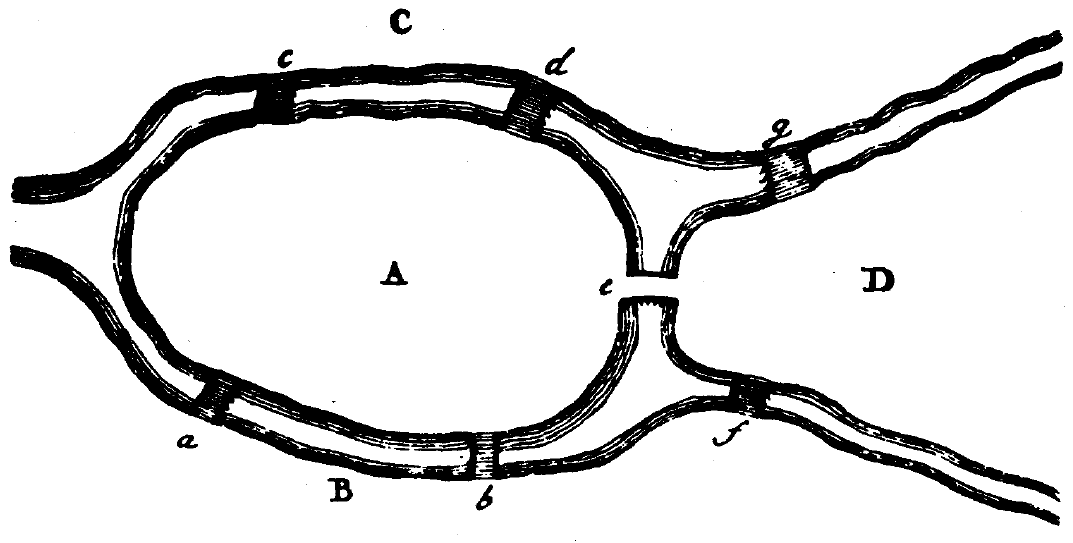
\includegraphics[width=\textwidth]{images/konigsberg.png}
		\subcaption{Rappresentazione dei ponti come descritta da Eulero.}
	\end{subfigure}
	\begin{subfigure}[b]{0.45\textwidth}
		\centering
		\begin{tikzpicture}
			\node[shape=circle,inner sep=2pt,draw,thick] (A) {A};
			\node[shape=circle,inner sep=2pt,draw,thick, below=of A] (B) {B};
			\node[shape=circle,inner sep=2pt,draw,thick, above=of A] (C) {C};
			\node[shape=circle,inner sep=2pt,draw,thick, right=of A] (D) {D};

			\draw[thick, bend left=10] (A) to (C);
			\draw[thick, bend right=10] (A) to (C);
			\draw[thick, bend left=10]  (A) to (B);
			\draw[thick, bend right=10] (A) to (B);
			\draw[thick]  (A) to (D);
			\draw[thick, bend left=10]  (C) to (D);
			\draw[thick, bend right=10]  (B) to (D);
		\end{tikzpicture}
		\subcaption{Rappresentazione come multigrafo.}
	\end{subfigure}
	\caption{I ponti di K\"onisberg.}
	\label{fig:ponti_konigsberg}
\end{figure}

Un antico problema chiedeva: è possibile partire da un punto qualsiasi della
città e attraversare tutti i ponti esattamente una ed una sola volta?
Per studiare questo problema, Eulero pensò di trasformare questa mappa in un
grafo, dove i vertici rappresentano le zone $A$, $B$, $C$, $D$ e i lati
sono i sette ponti della città. I grafi fatti in questo modo sono chiamati, oggi,
\textit{multigrafi}, ossia grafi i cui lati non sono un insieme ma un \textit{multinsieme},
insiemi con ripetizioni distinte: formalmenti, sono rappresentati con una mappa
che associa agli elementi il numero di ripetizioni. In termini di teoria dei
grafi, il problema si traduce come segue: $G$ ha un circuito (o ciclo)  che
passi esattamente una volta per ogni lato, ossia un \textbf{circuito euleriano}?

La risposta, in questo caso specifico, è no.
\begin{theorem}\label{thm:circ_euleriano}
	Esiste un circuito euleriano se e solo se tutti i vertici di un
	grafo connesso hanno grado pari.
\end{theorem}

\begin{proof}
	$\impliedby$ (Se tutti i vertici di un grafo hanno grado pari, allora esiste un
	circuito euleriano.) Sia $G$ un grafo in cui tutti i vertici hanno grado  pari.
	Partendo da un vertice a caso e seguendo un cammino formato da lati non
	ancora scelti (ossia si tiene traccia di quelli già ``consumati''), non può
	accadere che ci sia un arco non ancora scelto per planare sul nodo ma non
	un altro per uscirne, poiché questo significherebbe che il grado di tale nodo
	sia dispari.

	In questa costruzione succede, ad un certo punto, che si torna su uno
	dei vertici già visitati. Anche in questa situazione deve esistere un arco
	che permette di uscire da tale vertice: si segue quindi il lato non ancora
	utilizzato e si continua il percorso. Prima o poi, con questo ragionamento,
	si tornerà al vertice dal quale si è partiti, e questo è l'unico modo
	per costruire un circuito, che non è detto che sia euleriano, poiché non
	è detto che visiti tutti i lati. Tuttavia, si può ricominciare la visita partendo
	da un lato non ancora visitato: siccome il grafo è connesso, ci sarà modo
	di ricongiungersi al circuito iniziale.

\end{proof}

\noindent
Definiamo, invece, \textbf{circuito hamiltoniano} un circuto che passa esattamente una volta su ogni
vertice del grafo.

Un lemma utile è il seguente:
\begin{lemma}[Handshaking lemma]\label{lem:handshaking}
	In ogni grafo, il numero di vertici di grado dispari è pari.
\end{lemma}
\begin{proof}
	Deve essere
	$$
		\sum_{x \in V} d(x) = 2m
	$$
	ma la parità di una sommatoria dipende solo dai numeri dispari, infatti gli
	addendi pari non cambiano la parità. Se tale somma è pari, è necessario
	che il numero di addendi dispari sia pari.
\end{proof}


\noindent
Possiamo ora tornare al problema del commesso viaggiatore.

\popt {TravelingSalesman} {un grafo $G = (V,E)$ e un costo $\forall e \in E \delta_e$}
{Insieme ordinato di lati}
{Qual è il circuito hamiltoniano di minor costo?}
{Insieme ordinato di lati che formi un circuito hamiltoniano}
{$Min$}
{$\sum_{e \in \pi} \delta_e$}

\subsection{Algoritmo di Christofides}
\subsubsection{TSP su clique}
Si noti che non è necessario che esistano delle soluzioni ammissibili!
Per facilitare l'analisi e ottenere risultati migliori specializzeremo il problema in un certo modo:
analizzeremo il TSP su \textit{clique} (cricche), ossia un grafo
$G = (V, {V \choose{2}})$.

In quanto non è necessariamente vero che il grafo sia una cricca,
supponiamo di avere un grafo pesato non completo: lo trasformiamo in un
grafo completo
$$
	G = (V, E), \delta_e ~~ \leadsto ~~ K = (V, {V \choose 2}), \bar{\delta_e}
$$
definendo
$$
	\bar{\delta_e} =
	\begin{cases}
		\delta_e                    & e \in E    \\
		1 + \sum_{e \in E} \delta_e & e \notin E
	\end{cases}
$$
Se si trova una soluzione per $K$ che non utilizza nessun lato fittizio,
chiaramente tale soluzione è valida anche per $G$ ed è anche ottima, poiché
nessun circuito hamiltoniano può costare più di anche solo un lato fittizio.
In altre parole, la soluzione ottima coinvolge un lato fittizio se e solo se
per $K$ non vi sono soluzioni ammissibili.

\subsubsection{TSP metrico su clique}
Tuttavia, anche sulle clique il TSP è un problema estremamente complesso da
risolvere e, in generale, non è approssimabile a meno di una costante.
Con un ulteriore rilassamento riusciremo ad approssimare TSP, ossia
imponendo che le distanze formino una \textit{metrica} su $G$:
richiediamo che $G$ sia una cricca e $\delta_e$ sia una metrica, ossia $$
	\delta_{ij} \leq \delta_{ik} + \delta_{kj}
$$
% PROBLEMA: Se si crea il grafo completo utilizzando la costruzione precedente, la distanza 
% non è più una metrica..
Prima di designare l'algoritmo risolvente, introduciamo brevemente due problemi che
saranno utili.
\subsubsection{Minimo albero ricoprente}
\popt {MinimumSpanningTree} {$G = (V,E)$ \textit{bipartito}} {Insieme di lati}
{Qual è l'insieme di archi che copre i vertici con un costo minore?}
{L'insieme di lati è un albero, ossia un grafo connesso e aciclico}
{$Min$}{Cardinalità dell'insieme di lati}

Questo problema è risolvibile esattamente dall'algoritmo di Kruskal in tempo  $O(m\log(n))$.

\subsubsection{Matching perfetto a costo minimo}

\popt {MinimumWeightPerfectMatching} {$G = (V,E)$ con un numero pari di vertici}
{Insieme di lati}
{Esiste un matching perfetto?}
{Insieme di lati che formano un matching, ossia nessun vertice compare più di una volta, perfetto,
	ossia in cui compaiono tutti i vertici}
{$Min$}{Somma dei pesi degli archi scelti}

Anche questo problema è risolvibile in tempo polinomiale: un algoritmo famoso è
l'algoritmo \textit{dell'infiorescenza} che ha complessità $O(m \log(n))$.

\noindent
Possiamo ora passare all'algoritmo per risolvere istanze di \textsc{TravelingSalesman} su grafi
completi dotati di una distanza metrica.
\begin{algorithm}
	\caption{\textsc{ChristofidesTSP}}
	\KwInput{grafo $G = (V, {V \choose 2})$ con pesi $\delta_e$ che formano una metrica}

	$T = FindMST(G)$

	\tcc{$D$ è l'insieme dei vertici di grado dispari nel minimo albero ricoprente $T$. Per il
		\cref{lem:handshaking}, è $|D| \mod 2 = 0$.}
	$D = FindOddDegreeVertices(T)$

	\tcc{$G[D]$ è il grafo ristretto sui nodi di $D$}
	$G[D] = G(V \cap D, \cdots)$

	$M = FindPerfectMatching(G[D])$

	\tcc{\`E possibile che lo stesso lato appaia due volte, rendendo $H$ un multigrafo. Tutti i vertici
		in $H$ hanno grado pari, poiche' quelli che in $D$ hanno grado dispari hanno un nuovo lato.}
	$ H = T \cup M$

	$\pi = FindEulerianWalk(H)$

	$R = FindRepeatingVertices(\pi)$

	\For{$v : R$}
	{
		\tcc{per ogni vertice $v$ ripetuto nel cammino si cancellano due lati (uno entrante e uno uscente) e,
			siccome il grafo è una cricca, si inserisce un nuovo lato che collega i due vertici disconnessi
			(quello che portava a $v$ e quello raggiunto da $v$)}
		$\pi = RemoveAndReplace(\pi, v)$
	}

	\Return{$\pi$}
\end{algorithm}

\begin{lemma}\label{lem:tsp_T_leq_delta}
	Il costo dell'albero $T$ su $G$ è minore o uguale del costo ottimale del cammino hamiltoniano su $G$ metrico
	e completo:
	$$
		\delta(T) \leq \delta^*
	$$
\end{lemma}

\begin{proof}
	Sia $\pi^*$ un circuito hamiltoniano ottimo. Sia $e$ un qualunque lato che compare in $\pi^*$ e si
	consideri $\pi^* \setminus e$: il risultato è uno spanning tree (possibilmente minimo). Pertanto,
	$$
		\delta(T) \leq \delta(\pi^* \setminus e) \leq \delta^*
	$$
	poiché $T$ è \textit{un} minimo albero ricoprente.
\end{proof}
\begin{lemma}\label{lem:tsp_M_leq_hdelta}
	$$
		\delta(M) \leq \frac{1}{2}\delta^*
	$$
\end{lemma}
\begin{proof}
	Sia $\pi^*$ un circuito hamiltoniano ottimo.
	Dal \cref{lem:handshaking} sappiamo che un numero pari di vertici appare in $D$ come costruito
	nell'algoritmo: sia quindi $\pi'$ un qualunque circuito sui vertici di $D$.
	Questo circuito $\pi'$ attraverserà un numero minore o uguale di vertici attraversati da $\pi^*$,
	per ogni vertice in meno che deve attraversare dunque, invece di avere un lato che lo raggiunge
	ed uno da cui esce, ci sarà un solo lato che lo salta.
	Essendo $\delta$ una metrica dunque "saltare" un vertice dovrà costare per forza meno di prenderlo,
	quindi
	$$
		\delta(\pi') \leq \delta(\pi^*)
	$$
	Dividiamo i lati di $\pi'$ in due insiemi $M_1$ e $M_2$, in modo che si
	alternino nel cammino: essi sono due perfect matching su $D$. Allora
	\begin{align*}
		 & \delta(M_1) \geq \delta(M) \land \delta(M_2) \geq \delta(M)                      \\
		 & \implies \delta^* \geq \delta(\pi') = \delta(M_1) + \delta(M_2) \geq 2 \delta(M)
	\end{align*}
\end{proof}
\begin{theorem}
	L'algoritmo di Christofides è una $\frac{3}{2}$-approssimazione per il problema del
	commesso viaggiatore su grafi completi con distanza metrica.
\end{theorem}
\begin{proof}
	Siano $\tilde{\pi}$ il cammino hamiltoniano e $\pi$ il cammino euleriano costruiti dall'algoritmo.
	Allora deve essere $\delta(\tilde{\pi}) \leq \delta(\pi)$: $\pi$ passa per tutti
	gli archi di $H$ esattamente una volta:

	\begin{align*}
		 & \delta(\pi) = \sum_{e \in H} \delta(e)  = \delta(M) + \delta(T) \leq
		\underbrace{\frac{1}{2} \delta^*}_{\cref{lem:tsp_M_leq_hdelta}} +
		\underbrace{\delta^*}_{\cref{lem:tsp_T_leq_delta}}  = \frac{3}{2} \delta^*
	\end{align*}
\end{proof}

\begin{theorem}
	L'analisi di approssimazione  di TSP metrico su clique con Christofides è stretta.
\end{theorem}
\begin{proof}
	Dato $n$ pari ed $\epsilon \in (0,1)$, esibiamo il seguente grafo:

	\begin{figure}[h]
		\centering
		\begin{tikzpicture}
			\node[minimum size=15pt, draw, circle] (1) {$v_1$};
			\node[minimum size=15pt, draw, circle, right =of 1] (2) {$v_2$};
			\node[minimum size=15pt, draw, circle, right =of 2] (3) {$v_3$};
			\node[minimum size=15pt, draw, circle, right =of 3] (4) {$v_4$};
			\node[minimum size=15pt, draw, circle, right =of 4] (5) {$v_{n-2}$};
			\node[minimum size=15pt, draw, circle, right =of 5] (6) {$v_{n-1}$};
			\node[minimum size=15pt, draw, circle, right =of 6] (7) {$v_{n}$};

			\draw[] (1) to node [auto] {$1$} (2);
			\draw[bend right=35] (1) to node [below] {$1 + \epsilon$} (3);

			\draw[] (2) to node [auto] {$1$} (3);
			\draw[bend left=35] (2) to node [auto] {$1+\epsilon$} (4);

			\draw[] (3) to node [auto] {$1$} (4);
			\draw[bend right=30] (3) edge node [below] {$1 + \epsilon$}(5.5,-1);

			\draw[dotted] (4) to (5);

			\draw[] (5) to node [auto] {$1$} (6);
			\draw[bend left=35] (5) to node [auto] {$1+\epsilon$} (7);

			\draw[] (6) to node [auto] {$1$} (7);

			\draw[bend left=30] (6) edge node [auto] {$1 + \epsilon$} (7.5,-1);

		\end{tikzpicture}
	\end{figure}
	Tutti i lati mancanti hanno costo pari al costo del cammino minimo tra i due vertici del lato.
	L'algoritmo di Christofides seleziona il \textsc{MinimumSpanningTree} $T$, ossia il cammino composto da
	lati di costo $1$, quindi $\delta(T) = n - 1$. I nodi di grado dispari in $T$ sono
	i due estremi, quindi $D = \{v_1, v_n\}$. Il cammino minimo che li collega è
	un singolo lato che ha peso $\delta(M) = (1 + \epsilon) \frac{n}{2} + 1$.

	Al termine dell'algoritmo, il costo del circuito hamiltoniano ottenuto è
	$$
		\delta = n - 1 +  (1 + \epsilon) \frac{n}{2} + 1 = \frac{3}{2}n + \frac{\epsilon n}{2}
	$$
	Il costo del cammino ottimo è
	$$
		\delta^* = (1 + \epsilon) \frac{n}{2} + (1 + \epsilon) \frac{n}{2} +2 = (1 + \epsilon) n + 2
	$$
	quindi
	$$
		\frac{\delta}{\delta^*} = \frac{\frac{3}{2}n + \frac{\epsilon n}{2}}{(1 + \epsilon)n +2}
		= \frac{\frac{3}{2} n + \frac{n}{2}\epsilon}{n + 2 + \epsilon n} = \frac{3}{2}
	$$
	per $n \rightarrow \infty$ e $\epsilon \rightarrow 0$.
\end{proof}

% lezione 9 - 27/10/2021
\subsection{Inapprossimabilità di TSP}
La situazione non è altrettanto positiva per il caso generale del TSP:
\begin{theorem}
	Decidere se un grafo contiene un cammino hamiltoniano è un problema in $\mathbf{NP-completi}$.
\end{theorem}

\begin{theorem}
	Non esiste alcun $\alpha$ tale che \textsc{TravelingSalesman} sia $\alpha$-approssimabile a meno che
	$\mathbf{P} \neq \mathbf{NP}$.
\end{theorem}
\begin{proof}
	(per assurdo.)
	Sia $G = (V,E)$ un grafo che si completa creando $G'$: su questo grafo definiamo
	una nozione di distanza
	$$
		d(x,y) =
		\begin{cases}
			1                         & x, y \in E    \\
			\lceil \alpha n \rceil +1 & x, y \notin E
		\end{cases}
	$$
	Se $G$ ammette un circuito hamiltoniano, in $G'$ quel circuito ha costo
	$n$, poiché tocca tutti i vertici concludendo il circuito. Se $G$ non ammette
	un circuito hamiltoniano su di esso, possiamo concludere che in $G'$ tutti i
	circuiti hamiltoniani passano per almeno un lato di costo $\lceil \alpha n \rceil +1 $,
	quindi il circuito del costo hamiltoniano minimo è almeno $\lceil \alpha n \rceil + 1$.
	Se $G$ ha un circuito hamiltoniano l'algoritmo $\alpha$ approssimante per
	trovare cammini hamiltoniani in $G'$ (che, per assurdo, assumiamo esistere),
	troverà un circuito di costo minore o uguale a $\alpha n$ (poiché è $\alpha$-approssimante);
	se $G$ non ammette un circuito hamiltoniano, troverà un circuito di costo
	maggiore di $\lceil \alpha n \rceil +1$.
	\`E impossibile che $\alpha < \lceil \alpha n \rceil + 1$, altrimenti sapremmo
	decidere se $G$ ammette circuiti hamiltoniani. Ossia, deve essere
	$$
		\alpha > \frac{\lceil \alpha n \rceil + 1}{n} \geq \frac{\alpha n +1}{n} = \alpha + \frac{1}{n}
	$$
	ossia $\alpha \geq \alpha + \frac{1}{n}$, impossibile.
	Concludiamo che \textsc{TravelingSalesman} $\notin \mathbf{APX}$.
\end{proof}

\section{Problema del 2-carico}
In \textsc{LoadBalancing}, l'input era composto da  $t_0, t_1, \cdots, t_{n-1} \in \mathbb{N}^+$
tasks e un numero $m$ di macchine. L'obiettivo era costruire degli assegnamenti
tali per cui il carico massimo di una macchina è il minimo possibile. La versione
\textsc{$2$-LoadBalancing} è una specializzazione in cui $m = 2$.

\subsection{Algoritmo PTAS}
Due algoritmi per risolvere \textsc{LoadBalancing} sono stati proposti: greedy
(\cref{algo:greedybalance}) o con ordinamento iniziale delle task
(\cref{algo:sortedbalance}).
Ora, faremo molto meglio descrivendo un algoritmo che porta \textsc{$2$-LoadBalancing} in $\mathbf{PTAS}$:
daremo quindi un tasso di approssimazione vincolante per la soluzione trovata -
tuttavia l'algoritmo risulterà esponenziale in tale tasso.

\begin{algorithm}[h]
	\caption{PartitionBalance}
	\label{algo:partitionbalance}
	\KwInput{$m_1, m_2, t_0, ..., t_{n-1}, \epsilon$}

	\If {$\epsilon \geq 1$}
	{
		$m_1.tasks = \{t_0, \cdots, t_{n-1}\}$

		\Return
	}

	$tasks = [t_0,\cdots, t_{n-1}].nonDecreasingSort()$

	$k = \lceil \frac{1}{\epsilon} -1 \rceil$

	\tcc{Esegui l'algoritmo esaustivo sui primi $k$ task}
	$optPartition = findOptimalPartition(tasks[0\cdots k-1])$

	$GreedyBalance(m_1, m_2, tasks[k\cdots])$

\end{algorithm}

\begin{theorem}
	L'\cref{algo:partitionbalance} è polinomiale in $n$ (ma non in $\epsilon$) e
	produce una $1+ \epsilon$ approssimazione per \textsc{$2$-LoadBalancing}.
\end{theorem}

\begin{proof}
	Se $\epsilon \geq 1$, assegnare tutte le task ad una sola macchina non può
	essere peggio del doppio del costo ottimale.
	Altrimenti, proseguiamo seguendo l'esecuzione dell'algoritmo.
	I primi $k$ task vengono assegnati in modo ottimale. I seguenti $n - k$ task
	vengono assegnati in maniera greedy. Assumiamo, senza perdita di generalità,
	che $w(m_1) \geq w(m_2)$. Sia $h$ l'indice dell'ultimo task assegnato alla
	macchina $m_1$. Abbiamo due casi:
	\begin{itemize}
		\item $h < k$. Tutti i task assegnati in maniera greedy appartengono alla
		      macchina $m_2$. Siccome i task assegnati a $m_1$ sono assegnati in
		      modo ottimale, il costo massimo $w(m_1)$ è ottimale.
		\item $h \geq k$. Dopo la fase ottima la macchina $m_1$ riceve altri task.
		      Sia $L = \frac{\sum_{i} t_i}{2}$, facciamo due osservazioni che ci 
			  torneranno utili:
		      \begin{align*}
			       & w(m_1) - t_h  \leq w(m_2) \text{ nel momento in cui si assegna } h \leq w(m_2)                        \\
			       & \implies 2*w(m1) - t_h \leq w(m_1) + w(m_2) = 2L                                                      \\
			       & \implies w(m_1) - \frac{t_h}{2} \leq L
			  \end{align*}
			  e
			  \begin{align*}
				   & 2L  = t_0 + t_1 + \cdots + t_k + t_h + \cdots + t_{n-1} \geq t_h (k+1)                                \\
			  \end{align*}
			  Ora consideriamo il rapporto tra il valore restituito dall'algoritmo,
			  cioè il carico della macchina più carica (dunque $w(m_1)$). Ricordiamo che
			  $w^* \geq L$
			  \begin{align*}
				   & \frac{w}{w^*} = \frac{w(m_1)}{w^*} \leq \frac{w(m_1)}{L} \leq                                         \\
				   & \leq \frac{\frac{t_h}{2}+L}{L} = 1 + \frac{t_h}{2L} \leq & \text{per la prima osservazione}           \\
				   & \leq 1 + \frac{t_h}{2 \frac{t_h}{2} \cdot (k + 1)} = 1 + \frac{1}{1 + k} & \text{per la seconda osservazione} \\
		      \end{align*}
		      Ma $k = \lceil \frac{1}{\epsilon}\rceil - 1 \geq \frac{1}{\epsilon} - 1$, quindi:
		      \begin{align*}
				   & 1 + \frac{1}{1 + k} \leq 1 + \frac{1}{1 + \frac{1}{\epsilon} - 1} = 1 + \epsilon
		      \end{align*}
	\end{itemize}
\end{proof}

\begin{theorem}
	L'algoritmo ha tempo d'esecuzione $O(n\log{n} + 2^{\frac{1}{\epsilon}})$.
\end{theorem}
\begin{corollario}
	Essendo uguale a \textsc{2-LoadBalancing},  \textsc{MinimumPartition} $\in \mathbf{PTAS}$.
\end{corollario}

\section{Problema dello zaino}
\popt {Knapsack} {$n$ oggetti con valori $v_0, \cdots, v_{n-1} \in \mathbb{N}$ e
	pesi $w_0, \cdots, w_{n-1} \in \mathbb{N}$ e una capacità $W \in \mathbb{N}$} {Insieme di oggetti $S$}
{Qual è l'insieme di oggetti di valore maggiore che si può scegliere senza eccedere
	la capacità $W$?}
{Scelta di oggetti che non eccedono $W$: $\sum_{i \in S} w_i \leq W$}
{$Max$}{Valore degli oggetti in $S$: $\sum_{i \in S} v_i$}

\begin{theorem}
	\textsc{KnapsackProblem} $\in \mathbf{NPO-completi}$.
\end{theorem}

\subsection{Algoritmo esponenziale basato su programmazione dinamica}
Come solitamente accade quando si desidera trovare un algoritmo basato
sulla \textit{programmazione dinamica}, suddividiamo il problema in problemi
più piccoli: costruiamo una matrice
$$
	vOPT[i, w] =  \text{ massimo valore di } i \text{ oggetti con zaino di capacità } w
$$
con $ i \leq n$ e $w \leq W$. Ovviamente, ciò che ci interessa è $vOPT[n, W]$,
ossia il valore massimo ottenibile considerando tutti gli $n$ oggetti
e con capacità $W$.
In quanto il valore ottenibile scegliendo $0$ oggetti è $0$, abbiamo che, per qualsiasi
capacità, $vOPT[0, \_] = 0$ - analogamente, siccome nessun oggetto può essere scelto
se la capacità è $0$, deve essere $vOPT[\_, 0]  = 0$.

L'entry della $i+1$-esima riga nella $w+1$-esima colonna
si costruisce decidendo se inserire o meno l'$i$-esimo oggetto:
$$
	vOPT[i+1, w] =
	\begin{cases}
		vOPT[i, w]             & w_i > w    \\
		vOPT[i, w - w_i] + v_i & w_i \leq w
	\end{cases}
$$

Questo algoritmo, ovviamente, non può essere polinomiale (altrimenti sarebbe
$\mathbf{P} = \mathbf{NP}$) -- è vero che il
numero di entry nella matrice è $n \cdot w$, ma l'algoritmo non è polinomiale nella
lunghezza binaria dell'input $W$, bensì è esponenziale, rendendo quindi l'algoritmo
\textit{pseudopolinomiale}.

\subsection{Algoritmo FPTAS basato su programmazione dinamica}
Per cercare di ovviare al problema della pseudopolinomialità del metodo precedente,
scomponiamo il problema in termini di oggetti e valore (invece che peso):
$$
	wOPT[i, v] = \text{minimo peso necessario per i primi } i \text{ oggetti con valore } \geq v
$$
In $wOPT$ le colonne rappresentano valori tra $[0, \sum_{i}v_i]$ - in realtà,
approssimiamo questo range con $[0, n\cdot v_{max}]$, con $v_{max} = \max_i v_i$.

Sull'ultima riga troveremo il minimo peso necessario per scegliere $n$ oggetti;
potrà accadere che per molte colonne $wOPT[i,v] > W$, che rappresentanos
soluzioni non accettabilil; dovremo quindi cercare la prima entry che non sfora
la capacità $W$. La prima colonna sarà $wOPT[\_,0] = 0$, mentre, inizialmente,
si imposta $wOPT[0,\geq1] = \infty$.

La regola di riempimento che definiamo è
$$
	wOPT[i+1, v] = \min(wOPT[i, v], wOPT[i, \max(v-v_i, 0)] + w_i)
$$

Benché apparentemente sembra non ci sia alcun vantaggio, in questo frangente
possiamo operare delle modifiche sulla matrice: l'idea è quella di ``schiacciare''
le colonne, operando una divisione o un cambio di misura, nonostante venga
in questo modo introdotta un'approssimazione dei valori. Introduciamo,
quindi, un \textit{valore di scala}:
$$
	\theta = \frac{\epsilon v_{max}}{2n}
$$
e l'obiettivo finale sarà avere una $1+\epsilon$-approssimazione.
Sia quindi $X=(v_i, w_i, W)$ l'input del problema; siano

$$
	\bar{v_i} = \lceil\frac{v_i}{\theta}\rceil\cdot \theta, ~~ \hat{v_i} = \lceil \frac{v_i}{\theta}\rceil
$$
ai quali associamo i relativi problemi $\bar{X} = (\bar{v_i}, w_i, W)$
e $\hat{X} = (\hat{v_i}, w_i, W)$
che avranno delle soluzioni ottime $v^*, \bar{v}^*$ e $\hat{v}^*$, derivanti
da insiemi $S^*, \bar{S}^*$ e $\hat{S}^*$.

\begin{oss} \label{oss:knapsack_barv_t_hatv}
	Banalmente,
	$$
		\bar{v}^* = \theta \hat{v}^*
	$$
	In altre parole, risolvere $\hat{X}$ o risolvere $\bar{X}$ restituisce le
	stesse soluzioni, pertanto
	$$
		\bar{S}^* = \hat{S}^*
	$$

\end{oss}

\begin{lemma}
	Sia S una soluzione ammissibile per il problema. Allora
	$$
		(1+\epsilon)\sum_{i \in \hat{S}^*} v_i \geq \sum_{i \in \bar{S}^*} v_i
	$$
\end{lemma}
\begin{proof}
	\begin{align*}
		 & \sum_{i \in S} v_i \leq \sum_{i \in S} \bar{v}_i  \text{ grazie all'arrotondamento per eccesso}                      \\
		 & \leq \sum_{ i \in \bar{S}^*} \bar{v}_i  \text{ poiché è la soluzione ottima}                                         \\
		 & = \sum_{ i \in \hat{S}^*} \bar{v}_i \text{ poiché } \hat{S}^* = \bar{S}^* \text{ da \cref{oss:knapsack_barv_t_hatv}} \\
		 & = \sum_{i \in \bar{S}^*} \bar{v}_i \leq \sum_{i \in \hat{S}^*} (v_i + v) \leq
		\sum_{i \in \hat{S}^*} v_i + n \theta = \sum_{i \in \hat{S}^*} v_i + n \frac{\epsilon v_{max}}{2 n}
	\end{align*}
	quindi
	$$
		\sum_{i \in S} v_i  \leq \sum_{i \in \hat{S}^*} v_i + \frac{\epsilon v_{max}}{2}
	$$

	In particolare, questo vale per la soluzione composta
	solamente dall'oggetto con valore massimo $S = \{max\}$, da cui segue
	\begin{align*}
		 & v_{max} \leq \sum_{i \in \hat{S}^*} v_i + \frac{\epsilon v_{max}}{2}
		\leq \sum_{i \in \hat{S}^*} v_i + \frac{v_{max}}{2} \text{ poiché } \epsilon \leq 1         \\
		 & \implies \sum_{i \in \hat{S}^*} v_i \geq \frac{v_{max}}{2}                               \\
		 & \implies \sum_{i \in S} v_i \leq \sum_{i \in \hat{S}^*} v_i + \frac{\epsilon v_{max}}{2}
		\leq \sum_{i \in \hat{S}^*}v_i + \epsilon \sum_{i \in \hat{S}^*} v_i = (1 + \epsilon) \sum_{i \in \hat{S}^*} v_i
	\end{align*}
\end{proof}
\begin{theorem}
	$$
		(1+\epsilon)\sum_{i \in \hat{S}^*} v_i \geq \sum_{i \in S^*} v_i = v^*
	$$
	Risolvendo il problema $\hat{X}$ si ottiene una soluzione il cui valore
	per il problema originale è
	$\frac{1}{1+\epsilon}$
	volte l'ottimo.
\end{theorem}

\begin{algorithm}
	\caption{FPTASKnapsack}
	\label{algo:FPTASKnapsack}
	\KwInput{$X = (v_i, w_i, W), \epsilon$}

	$
		\hat{X} = getFrom(X, \epsilon)
	$

	\tcc*{La soluzione così trovata è una $(1 + \epsilon)-$approssimazione}

	\Return {$solveWithWOpt(\hat{X})$}
\end{algorithm}

Dobbiamo ora convincerci che \cref{algo:FPTASKnapsack} termini
in tempo polinomiale: l'ultima colonna sarà $n \hat{v}_{max}$;
sappiamo che
$$
	v_{max} = \lceil \frac{v_{max}}{\theta} \rceil = \lceil \frac{v_{max} n}{\epsilon v_{max}} \rceil
	=\lceil \frac{n}{\epsilon}\rceil
$$
pertanto il numero di colonne
$$
	n\hat{v}_{max} \leq \frac{n^2}{\epsilon} + n
$$
polinomiale nell'input e in $\epsilon$.




%%% Local Variables:
%%% TeX-master: "../main"
%%% End:

% lezione 10 - 03/11/2021
\chapter{Algoritmi probabilistici}
Fino ad ora abbiamo considerato il modello di calcolo delle macchine di Turing per
scrivere algoritmi per problemi di ottimizzazione, in particolare algoritmi di
approssimazione:
% disegno: input x -> MdT A -> output y
\begin{figure}[h]


	\centering

	\tikzset{every picture/.style={line width=0.75pt}} %set default line width to 0.75pt        

	\begin{tikzpicture}[x=0.75pt,y=0.75pt,yscale=-1,xscale=1]
		%uncomment if require: \path (0,437); %set diagram left start at 0, and has height of 437

		%Rounded Rect [id:dp7665142760923608] 
		\draw   (280,152) .. controls (280,145.37) and (285.37,140) .. (292,140) -- (358,140) .. controls (364.63,140) and (370,145.37) .. (370,152) -- (370,188) .. controls (370,194.63) and (364.63,200) .. (358,200) -- (292,200) .. controls (285.37,200) and (280,194.63) .. (280,188) -- cycle ;
		%Straight Lines [id:da12014265713573546] 
		\draw    (170,170) -- (277,170) ;
		\draw [shift={(280,170)}, rotate = 180] [fill={rgb, 255:red, 0; green, 0; blue, 0 }  ][line width=0.08]  [draw opacity=0] (8.93,-4.29) -- (0,0) -- (8.93,4.29) -- cycle    ;
		%Straight Lines [id:da500409813700509] 
		\draw    (370,170) -- (477,170) ;
		\draw [shift={(480,170)}, rotate = 180] [fill={rgb, 255:red, 0; green, 0; blue, 0 }  ][line width=0.08]  [draw opacity=0] (8.93,-4.29) -- (0,0) -- (8.93,4.29) -- cycle    ;

		% Text Node
		\draw (311,162) node [anchor=north west][inner sep=0.75pt]   [align=left] {MdT};
		% Text Node
		\draw (214,152) node [anchor=north west][inner sep=0.75pt]   [align=left] {input};
		% Text Node
		\draw (404,152) node [anchor=north west][inner sep=0.75pt]   [align=left] {output};


	\end{tikzpicture}
	\caption{Macchina di Turing deterministica}
	\label{fig:mdtdet}
\end{figure}
gli algoritmi sono quindi \textbf{deterministici}, nonostante in alcune situazioni
gli algoritmi possano fare scelte ``arbitrarie'', che formalizziamo con la nozione
di gradi di libertà - abbiamo tuttavia dimostrato che le proprietà sono
indipendenti da queste scelte arbitrarie.

Dobbiamo riservare il termine di \textbf{non determinismo} per definire
classi di complessità per modelli di calcolo \textit{non realistici}. Estendiamo
ora il modello: abbiamo una MdT che è anche in grado di leggere un nastro su
cui sono scritti dei valori casuali, chiamato \textbf{sorgente aleatoria}.
%          sorgente aleatoria one way
%                      |
%                      v 
% disegno: input x -> MdT A -> output y
\begin{figure}[h]
	\centering



	\tikzset{every picture/.style={line width=0.75pt}} %set default line width to 0.75pt        

	\begin{tikzpicture}[x=0.75pt,y=0.75pt,yscale=-1,xscale=1]
		%uncomment if require: \path (0,437); %set diagram left start at 0, and has height of 437

		%Rounded Rect [id:dp7665142760923608] 
		\draw   (280,152) .. controls (280,145.37) and (285.37,140) .. (292,140) -- (358,140) .. controls (364.63,140) and (370,145.37) .. (370,152) -- (370,188) .. controls (370,194.63) and (364.63,200) .. (358,200) -- (292,200) .. controls (285.37,200) and (280,194.63) .. (280,188) -- cycle ;
		%Straight Lines [id:da12014265713573546] 
		\draw    (170,170) -- (277,170) ;
		\draw [shift={(280,170)}, rotate = 180] [fill={rgb, 255:red, 0; green, 0; blue, 0 }  ][line width=0.08]  [draw opacity=0] (8.93,-4.29) -- (0,0) -- (8.93,4.29) -- cycle    ;
		%Straight Lines [id:da500409813700509] 
		\draw    (370,170) -- (477,170) ;
		\draw [shift={(480,170)}, rotate = 180] [fill={rgb, 255:red, 0; green, 0; blue, 0 }  ][line width=0.08]  [draw opacity=0] (8.93,-4.29) -- (0,0) -- (8.93,4.29) -- cycle    ;
		%Straight Lines [id:da29880468042507347] 
		\draw    (330,62.29) -- (330,137) ;
		\draw [shift={(330,140)}, rotate = 270] [fill={rgb, 255:red, 0; green, 0; blue, 0 }  ][line width=0.08]  [draw opacity=0] (8.93,-4.29) -- (0,0) -- (8.93,4.29) -- cycle    ;

		% Text Node
		\draw (311,162) node [anchor=north west][inner sep=0.75pt]   [align=left] {MdT};
		% Text Node
		\draw (214,152) node [anchor=north west][inner sep=0.75pt]   [align=left] {input};
		% Text Node
		\draw (404,152) node [anchor=north west][inner sep=0.75pt]   [align=left] {output};
		% Text Node
		\draw (347,72) node [anchor=north west][inner sep=0.75pt]   [align=left] {sorgente aleatoria};
		% Text Node
		\draw    (178,37) -- (491,37) -- (491,62) -- (178,62) -- cycle  ;
		\draw (181,41) node [anchor=north west][inner sep=0.75pt]   [align=left] { 0 1 0 1 1 1 0 0 1 1 1 1 1 1 0 0 1 0 1 0 1 1 1 1 ...};


	\end{tikzpicture}
	\caption{Macchina di Turing probabilistica}
	\label{fig:mdtprob}
\end{figure}

Un algoritmo così costruito è definito \textbf{probabilistico}, in quanto l'output
sarà in funzione dell'input e del seme casuale. L'algoritmo possiede quindi
una certa distribuzione associata
$$
	P[Y = y | X = x]
$$
ossia la probabilità di avere l'output $y$ per un input $x$. Gli algoritmi
probabilistici si dividono in due famiglie:
gli algoritmi \textbf{Monte-Carlo} in cui l'output è probabilistico e gli algoritmi
\textbf{Las Vegas}, in cui l'output è deterministico, ma il tempo di esecuzione
è probabilistico. In particolare, studieremo la prima famiglia.

Questo modello di calcolo
si può applicare sia a problemi di decisione che di ottimizzazione; per applicare
questi algoritmi, vi sono due varianti: nel primo caso l'algoritmo mira ad
ottenere l'ottimo con una certa probabilità, idealmente alta - essi possono
tuttavia fallire arbitrariamente male. Alternativamente, l'algoritmo può
mirare a ottenere un'\textit{approssimazione} dell'ottimo con una certa
probabilità.

\section{Problema del taglio minimo}
\popt {MinimumCut} {$G = (V,E)$} {Sottoinsieme $X \subseteq V$}
{Qual è il \textit{taglio} minore?}
{
	$X \subseteq V$ tale che il numero di lati che hanno un vertice in $X$ e un vertice
	in $X^c$ (\textit{tagliati}) è minimo;
	definiamo
	$E_X = \{e | e \cap X \neq \emptyset \land e \cap X^* \neq \emptyset\}$
}
{$Min$}{$|E_x|$}


Le soluzioni banali sono $X = V$ e $X = \emptyset$; inoltre, una soluzione
sempre possibile è scegliere $X = \{ v \}$ per un qualsiasi $v \in V$.

\begin{theorem}
	\textsc{MinimumCutProblem} $\in \mathbf{NPO-completi}$
\end{theorem}

\subsection{Algoritmo di Karger}
L'algoritmo di Karger utiliza l'operazione di \textit{contrazione}: dato un
grafo $G$, l'operazione $G \downarrow e$ su un lato $e = \{u, v\} \in E$
unisce i due vertici $u$ e $v$, rimuovendo $e$.
\begin{figure}[h]
	\begin{center}
		\begin{tikzpicture}[scale=1, transform shape]
			\node[draw,inner sep=0pt,minimum size=5pt,fill, circle] at (0, 2)  (u1) {};
			\node[draw,inner sep=0pt,minimum size=5pt,fill, circle] at (-1, 2)  (u2) {};
			\node[draw,inner sep=0pt,minimum size=5pt,fill, circle] at (1, 2)  (u3) {};
			\node[draw,inner sep=0pt,minimum size=5pt,fill, circle, label={0:u}] at (0, 0)  (a) {};
			\node[draw,inner sep=0pt,minimum size=5pt,fill, circle, label={0:v}] at (0, 1)  (b) {};
			\node[draw,inner sep=0pt,minimum size=5pt,fill, circle] at (0, -1)  (l1) {};
			\node[draw,inner sep=0pt,minimum size=5pt,fill, circle] at (-1, -1)  (l2) {};
			\node[draw,inner sep=0pt,minimum size=5pt,fill, circle] at (1, -1)  (l3) {};

			\draw (u1) -- (b);
			\draw (u2) -- (b);
			\draw (u3) -- (b);

			\draw (l1) -- (a);
			\draw (l2) -- (a);
			\draw (l3) -- (a);


			\node at (1.75,0.5) (to) {$\implies$};
			\draw (a) edge node [left] {e} (b);
			\node[draw,inner sep=0pt,minimum size=5pt,fill, circle] at (3.5, 1.5)  (lu1) {};
			\node[draw,inner sep=0pt,minimum size=5pt,fill, circle] at (2.5, 1.5)  (lu2) {};
			\node[draw,inner sep=0pt,minimum size=5pt,fill, circle] at (4.5, 1.5)  (lu3) {};
			\node[draw,inner sep=0pt,minimum size=5pt,
			fill, circle, label={0:{u,v}}] 			at (3.5, 0.5)  (la) {};
			\node[draw,inner sep=0pt,minimum size=5pt,fill, circle] at (3.5, -0.5)  (ll1) {};
			\node[draw,inner sep=0pt,minimum size=5pt,fill, circle] at (2.5, -0.5)  (ll2) {};
			\node[draw,inner sep=0pt,minimum size=5pt,fill, circle] at (4.5, -0.5)  (ll3) {};
			\draw (lu1) -- (la);
			\draw (lu2) -- (la);
			\draw (lu3) -- (la);
			\draw (ll1) -- (la);
			\draw (ll2) -- (la);
			\draw (ll3) -- (la);
		\end{tikzpicture}
	\end{center}
	\caption{Contrazione $G\downarrow e$.}
	\label{fig:contrazione}
\end{figure}

\`E necessario che $G$ sia
un multigrafo, poiché unendo $u$ e $v$ è possibile che un terzo vertice $y$
fosse collegato sia a $u$ che a $v$; rimarranno quindi dei lati paralleli.
In caso il lato contratto fosse uno dei lati paralleli tra $u$ e $v$ anche
i lati paralleli rimanenti vengono contratti.

\begin{algorithm}[h]
	\caption{\textsc{KargerMinimumCut}}
	\label{algo:Karger}
	\KwInput{$G = (V,E)$}

	\If{$\neg G.isConnected()$}
	{
		\Return{$findConnectedComponent(G)$}
	}
	\While{$|V| > 2$}
	{
		\tcc*{Estrai un lato con una distribuzione uniforme e contrailo}
		$e = uniformExtraction(E)$

		$G = G\downarrow e$

	}

	\tcc*{Restituisci uno dei due vertici rimanenti}
	\Return{$chooseOne(V)$}

\end{algorithm}

Chiaramente, l'output dipende dalla scelta dei lati da contrarre, che è casuale.
Sia quindi $S^*$ il taglio minimo, $k^*$ il numero di lati tagliati da $S^*$ e
la serie $G_1, \cdots, G_i$ la sequenza di grafi ottenuti per ogni contrazione
operata dall'algoritmo.
\begin{oss}\label{oss:kargercontraction}
	$\forall i ~~ |G_i(V)| = n - i + 1 \land |G_i(E)| \leq m - i + 1$
\end{oss}
\begin{oss}\label{oss:kargercuts}
	Per ogni $i$, ogni taglio in $G_i$ è un taglio in $G$ dello stesso costo.
\end{oss}
\begin{oss}\label{oss:kargermindeg}
	Il grado minimo in $G_i$ è maggiore o uguale a $k^*$.
\end{oss}

\begin{lemma}\label{lem:kargeredges}
	$m - i  +1 \geq \frac{(n - i + 1) \cdot k^*}{2}$
\end{lemma}
\begin{proof}
$$
	2(m - i +1) \geq 2 \cdot |G_i(E)| = \sum_{v \in G_i(V)} d_{G_i}(v) \geq k^* (n - i + 1) \implies m - i  +1 \geq \frac{(n - i + 1) \cdot k^*}{2}
$$
\end{proof}

\begin{lemma}\label{lem:kargerprob_ei}
	Sia $E_i$ l'evento ``al passo $i$-esimo un lato $e \notin E_{S^*}$ viene contratto''.
	$$
		\forall i ~~ P[E_i | E_1, \cdots, E_{i-1}] \leq \frac{n-i-1}{n-i+1}
	$$
\end{lemma}
\begin{proof}
	\begin{align*}
		P[E_i | E_1, \cdots, E_{i -1}] & = 1 - P[\neg E_i | E_1, \cdots, E_{i -1}]           		\\
		 & = 1 - \frac{k^*}{|G_i(V)|}  																\\
		 & \geq 1 - \frac{k^*}{m - i + 1} && \text{per \cref{oss:kargercontraction}} 				\\
		 & \geq 1 - \frac{2 \cdot k^*}{k^* \cdot (n - i  + 1)} && \text{per \cref{lem:kargeredges}} \\
		 & = 1 - \frac{2}{n - i + 1} = \frac{n - i -  1}{n - i + 1}
	\end{align*}
\end{proof}

\begin{theorem}
	L'algoritmo di Karger emette l'ottimo con probabilità $p \geq \frac{1}{{n\choose{2}}}$.
\end{theorem}
\begin{proof}
	Una esecuzione dell'algoritmo che emette l'ottimo vuol dire che, ad ogni
	passo, ha selezionato un lato da contrarre $e \notin E_{S^*}$. Siamo dunque
	interessati alla probabilità dell'evento
	$E_1 \land E_2 \land \cdots \land E_{n-2}$:
	\begin{align*}
		P[E_1 \land E_2 \land \cdots \land E_{n-2}] & = P[E_1] \cdot P[E_2|E_1] \cdot \cdots \cdot P[E_{n-2}| E_{n-3}, \cdots, E_1] 				\\
		& \geq \frac{n-1-1}{n-1+1} \cdot \frac{n-2-1}{n-2+1} \cdot \cdots \cdot \frac{n-(n-2)-1}{n-(n-2)+1} & \text{applico \cref{lem:kargerprob_ei}}  \\
		& = \frac{n-2}{n} \cdot \frac{n-3}{n-1} \cdot \cdots \cdot \frac{1}{3}																		\\
		& = \frac{\Pi_{i = 1}^{n-2} i}{\Pi_{i = 3}^{n} i} = \frac{2 \cdot 1}{n \cdot (n-1)} = \frac{2}{n (n-1)} = \frac{1}{{n\choose{2}}}
	\end{align*}
\end{proof}

\begin{oss}
	Si esegua l'algoritmo di Karger ${n\choose{2}} \log(n)$ volte.
	L'ottimo si ottiene con probabilità $p \geq 1 - \frac{1}{n}$.
\end{oss}
\begin{proof}
	Ad ogni esecuzione dell'algoritmo, la probabilità di non trovare l'ottimo è
	$$
		p \leq \left(1 - \frac{1}{{n \choose{2}}}\right)
	$$
	Di conseguenza, se eseguiamo l'algoritmo ${n \choose{2}} log(n)$ volte,
	la probabilità che nessuna di queste esecuzioni trovi l'ottimo è
	$$
		p \leq \left(1 - \frac{1}{{n \choose 2}}\right)^{{n \choose{2}}log(n)}
	$$
	\'E facilmente dimostrabile, osservando il grafico della funzione, che vale
	la seguente proprietà:
	$$
		\forall x \geq 1 \text{ interi } ~~ \frac{1}{4} \leq ( 1 - \frac{1}{x})^x \leq \frac{1}{e}
	$$
	Applicando la disuguaglianza alla nostra proprietà, con $x={n \choose{2}}$
	ed elevando entrambi i lati per $log(n)$, otteniamo
	$$
		p \leq \left( 1 - \frac{1}{{n \choose 2}}\right) ^{{n \choose 2} \log (n)} \leq \left(\frac{1}{e}\right)^{\log(n)} = \frac{1}{n}
	$$
	In questo caso $p$ è la probabilità di \textit{non} trovare l'ottimo,
	dunque la probabilità di trovarlo è $\geq 1 - \frac{1}{n}$
\end{proof}

\section{Problema della copertura d'insiemi}
Abbiamo già definito il \textsc{SetCoverProblem}:
dato una serie di insiemi
$$
	S_1, \cdots, S_m \subseteq U
$$
con pesi
$$
	w_1 \cdots, w_m \in \mathbb{Q}^+
$$
definiamo $n = |U|$; vogliamo trovare un $S \subseteq m$ tale che
$$
	\bigcup_{i \in S} S_i = U
$$
e il suo costo $ \sum_{i \in S} w_i$ sia minimo.

\subsection{Algoritmo probabilistico basato sull'arrotondamento}
Il problema può essere trasposto in un problema di programmazione lineare intera:
creiamo delle variabili
$$
	x_1, \cdots, x_m
$$
tali che
$$
	\begin{cases}
		x_j \leq 1                     & \forall j = 1, \cdots, m \\
		x_j \geq 0                     & \forall j = 1, \cdots, m \\
		\sum_{i: u \in S_i} x_i \geq 1 & \forall u \in U
	\end{cases}
$$
Come sappiamo, i problemi di programmazione lineare intera appartengono alla
classe \textbf{NP-Completi}. Consideriamo dunque il problema $\Pi$ nella
sua versione non intera, $\Pi_{PL}$.

\`E importante richiamare ora alcune proprietà statistiche.
\begin{theorem}[Disuguaglianza di Markov]\label{thm:markov}
	Per ogni variabile aleatoria $X$ non negativa e per ogni $\alpha > 0$
	$$
		P[X \geq \alpha] \leq \frac{E[X]}{\alpha}
	$$
\end{theorem}

\begin{theorem}[Union bound o disuguaglianza di Boole]\label{thm:boole}
	$$
		P[\bigcup_{i} E_i] \leq \sum_i P[E_i]
	$$
\end{theorem}

\begin{algorithm}[h]
	\caption{\textsc{ProbabilisticRoundingSetCover}}
	\label{algo:ProbRoundingSetCover}
	\KwInput{$S_1, \cdots, S_m$, $w_1, \cdots, w_m$  e un intero $k$}

	$\hat{x_1}, \cdots, \hat{x_m} = solve(\Pi_{PL}) $

	$S =  \emptyset$

	\For {$t = \{1, \lceil k + \log(n) \rceil \}$}
	{

		\For {$i = 1, ..., m$}
		{
			\tcc*{Inserisci $i$ in $S$ con probabilità $\hat{x_i}$}
			$S = probInsert(S, i, \hat{x_i})$
		}
	}

	\Return {$S$}
\end{algorithm}

L'\cref{algo:ProbRoundingSetCover} potrebbe trovare una soluzione non ammissibile. Dimostriamo
ora che \textit{spesso} è ammissibile e che quando è ammissibile è una soluzione molto buona.

\begin{theorem}
	La probabilità che l'\cref{algo:ProbRoundingSetCover} produca una soluzione ammissibile è
	$$
		p \geq 1 - e ^ {-k}
	$$
	parametrica in $k$, che determina il numero di tentativi di inserimento.
\end{theorem}
\begin{proof}
	$$
		P[\text{soluzione ammissibile}] = 1 - P[\text{almeno un elemento dell'universo non è coperto}]
	$$
	chiamiamo $B_u$ l'evento per cui $u$ non è coperto nella soluzione. Allora
	$$
		P[\text{soluzione ammissibile}] = 1 - P[\bigcup_{u \in U} B_u]
	$$
	Possiamo quindi usare il \cref{thm:boole}:
	$$
		1 - P[\bigcup_{u \in U} B_u] \geq 1 - \sum_{u \in U} P[B_u]
	$$
	L'elemento $u$ non è coperto quando nessuno degli elementi che contentono
	$u$ non è stato scelto. Ad ogni iterazione, che sono
	$\lceil k + \log(n) \rceil$ in totale, ogni insieme ha probabilità
	$\hat{x_i}$ di essere scelto:
	\begin{align*}
		1 - \sum_{u \in U} \prod_{i: u \in S_i} P[S_i \text{ non è stato scelto}] & = 1 - \sum_{u \in U} \prod_{i: u \in S_i} (1 - \hat{x_i})^{\lceil k + \log(n) \rceil}	\\
		& \geq 1 - \sum_{u \in U} \prod_{i : u \in S_i} e^{-\hat{x_i} (k + \log(n))} & \text{nota che } 1 - x \leq e^{-x}													\\
		& = 1 - \sum_{u \in U} \exp(- (k + \log (n)) \sum_{i: u \in S_i} \hat{x_i})
	\end{align*}
	Siccome $S_i$ è ammissibile, deve essere $\sum_{i: u \in S_i} \hat{x_i}  \geq 1$, quindi
	\begin{align*}
		\geq 1 - \sum_{u \in U} e^{- (k + \log(n))} = 1 - \sum_{u \in U} \frac{e^{-k}}{n}  = 1 - e^{-k} \frac{1}{n}|U| = 1 - e^{-k}
	\end{align*}
\end{proof}

\begin{theorem} \label{thm:ProbRoundingSetCoveralpha}
	$$\forall \alpha  ~~ 0 \leq \alpha \leq 1 ~~ P[\frac{v_{out}}{v^*}\geq \alpha (k + \log(n))] \leq \frac{1}{\alpha}$$
\end{theorem}
\begin{proof}
	Abbiamo che $\hat{v} = \sum_{i} w_i \hat{x_I} \leq v^*$; inoltre,
	la probabilità che $S_i$ venga scelto è

	\begin{align*}
		P[ S_i \text{ sia scelto}] & = P[ \bigcup_{t} S_i \text{ sia scelto durante l'iterazione } t] 	\\
		& \leq \sum_t P[S_i \text{ sia scelto durante l'iterazione } t] & \text{per \cref{thm:boole}}	\\ 
		& = (k + \log (n))\hat{x}_i
	\end{align*}

	Per poter utilizzare il \cref{thm:markov} calcoliamo il valore atteso di $v_{out}$:
	\begin{align*}
		E[v_{out}] & = \sum_{i} w_i P[S_i \text{ sia scelto}] 							\\
		& \leq \sum_i w_i (k + \log(n)) \hat{x_i} & \text{per osservazione precedente} 	\\
		& = \hat{v} (k + \log(n)) & \text{ricorda che } \hat{v}=\sum_i w_i \hat{x_i} 	\\
		& \leq v^* (k + \log(n))
	\end{align*}

	Infine utilizziamo questa osservazione per determinare la probabilità che
	la nostra soluzione approssimi bene il problema:
	\begin{align*}
		P [ \frac{v_{out}}{v^*} \geq \alpha (k + \log(n))] & = P [ v_{out} \geq v^* \alpha (k + \log(n)) ] 	\\
		& \leq \frac{E[v_{out}]}{\alpha (k + \log(n))v^*} & \text{applico Markov} 							\\
		& \leq \frac{v^* (k + \log(n))}{\alpha (k + \log(n))v^*} & \text{applico l'osservazione precedente}	\\ 
		& = \frac{1}{\alpha}		
	\end{align*}
\end{proof}

\begin{oss}
	Se si esegue l'\cref{algo:ProbRoundingSetCover} con $k = 3$ c'è il $45\%$ di probabilità di ottenere
	una soluzione ammissibile con fattore di approssimazione $\frac{v_{out}}{v^*}\leq 6 + 2 \log (n)$.
\end{oss}
\begin{proof}
	Sia $E_{ammissibile}$ l'evento per cui si ottiene una soluzione ammissible e
	$E_{buona}$ l'evento per cui l'output sia entro $6 + 2 \log(n)$ dall'ottimo.
	Ci interessa
	\begin{align*}
		 & P[E_{ammissibile} \land E_{buona}] = 1 - P[\neg E_{ammissible} \lor
		\neg E_{buona}] \geq 1 - P[\neg E_{ammissibile}] - P[\neg E_{buona}]                                  \\
		 & \geq 1 - e^{-3} - \frac{1}{2} \approx 0.45  ~~~  (\text{dal \cref{thm:ProbRoundingSetCoveralpha}})
	\end{align*}
\end{proof}

% lezione 13 - 10-11-2021 
\section{Problema MaxEkSat}
\textsc{MaxEkSat} è la versione $k$-indicizzata di \textsc{MaxSat}: date $t$ clausole
di $k$ letterali ciascuna, l'obiettivo è massimizzare il numero di clausole
soddisfatte.

Definiamo $x_1, \cdots, x_n$ le variabili che compaiono nella formula
e $c_1, \cdots, c_t$ le clausole della formula.

\begin{theorem}\label{thm:maxeksatnp}
	\textsc{MaxEkSat} $\in \mathbf{NPO-completi}$ per $k \leq 3$.
\end{theorem}

\subsection{Algoritmo probabilistico}
\begin{theorem}\label{thm:probassgn}
	Assegnando casualmente le variabili, il valore atteso di clausole soddisfatte è
	$$
		E[T] = \frac{2^k-1}{2^k} t
	$$
\end{theorem}
\begin{proof}
	Per la dimostrazione definiamo
	$$
		X_i \sim Unif(\{0,1\})
	$$
	il valore assegnato ad ogni $x_i$ probabilisticamente;
	$$
		C_i =
		\begin{cases}
			1 & C_i \text{ soddisfatto} \\
			0 & \text{ altrimenti}
		\end{cases}
	$$
	mentre $T=\sum_i^t C_i$ è il numero di clausole soddisfatte.
	L'algoritmo si svolge, banalmente, estraendo un valore per ogni $x_i$
	e restituendo il numero di clausole soddisfatte.

	\begin{oss}\label{oss:ciatteso}
		$$
			\forall i ~ \sum_{b_1 \in 2} \sum_{b_2 \in 2} \cdots \sum_{b_n \in 2} E[C_i | X_1=b_1 \cdots x_n=b_n] = 2^n - 2^{n - k}
		$$
	\end{oss}
	\begin{proof}
		Consideriamo una generica clausola $c_i$ e la sua variabile aleatoria
		associata $C_i$. Una volta che è stato fissato un assegnamento di
		valori di verità $b_1 \cdots b_n$, il valore di
		$E[C_i | X_1=b_1 \cdots x_n=b_n]$ sarà semplicemente $1$ o $0$, in base
		a se quell'assegnamento soddisfa la clausola $c_i$ o meno.

		Possiamo dunque vedere
		$$
			\sum_{b_1 \in 2} \sum_{b_2 \in 2} \cdots \sum_{b_n \in 2} E[C_i | X_1=b_1 \cdots x_n=b_n]
		$$
		semplicemente come il numero di assegnamenti che soddisfano la clausola
		$c_i$.
		Per contare questo numero, consideriamo che il valore di verità di una
		clausola dipende solamente dai valori delle $k$ variabili che contiene
		al suo interno, le altre $n-k$ variabili non sono importanti.
		Essendo questi $k$ letterali tutti in $\vee$ tra di loro, se uno di
		questi è \textit{True} allora l'intera clausola è soddisfatta.

		Vedendo questa osservazione all'opposto, per rendere la clausola falsa
		dobbiamo fissare le $k$ variabili con un assegnamento specifico per
		rendere tutti i loro letterali \textit{False}, e le rimanenti $n-k$
		variabili possono assumere qualunque valore. Da questo otteniamo
		che ci sono $2^{n-k}$ assegnamenti che \textit{non} soddisfano la
		clausola, dunque ne esistono $2^n - 2^{n-k}$ che la soddisfano.
	\end{proof}

	Prima di procedere con la dimostrazione, ricordiamo la seguente legge
	statistica:
	\begin{theorem}\label{thm:leggevat}
		Sia $\{\mathcal{E}_i\}_{i=1..k}$ una partizione dell'universo degli eventi.
		Allora
		$$
			E[X] = \sum_{i = 1}^{k} E[X|\mathcal{E}_i]P[\mathcal{E}_i]
		$$
	\end{theorem}

	La partizione $\{\mathcal{E}_i\}_i$ nel contesto di \textsc{MaxEkSat} è l'insieme
	dei possibili assegnamenti $X_1 = b_1, \cdots, X_n = b_n$; pertanto
	\begin{align*}
		E[T] & = \sum_{b_1 \in 2} \cdots \sum_{b_n\in 2} E[T|X_i = b_1, \cdots, X_n = b_n]P[X_1 = b_1, \cdots, X_n = b_n]   											\\
		     & = \sum_{b_1 \in 2} \cdots \sum_{b_n\in 2} E[T|X_i = b_1, \cdots, X_n = b_n]P[X_1 = b_1] \cdots P[X_n = b_n]  											\\
		     & = \frac{1}{2^n}\sum_{b_1 \in 2} \cdots \sum_{b_n\in 2} E[T|X_i = b_1, \cdots, X_n = b_n]                     											\\
			 & = \frac{1}{2^n}\sum_{b_1 \in 2} \cdots \sum_{b_n \in 2} E[C_1 + ... + C_t | X_i = b_1, \cdots, X_n = b_n] & \text{Per definizione di T}					\\
		     & = \frac{1}{2^n}\sum_{j = 1}^{t}(\sum_{b_1 \in 2} \cdots \sum_{b_n\in 2} E[C_j|X_i = b_1, \cdots, X_n = b_n]) & \text{Per linearità del valore atteso} 	\\
		     & = \frac{1}{2^n} \sum_{j = 1}^t (2^n - 2^{n -k}) = \frac{2^n - 2^{n-k}}{2^n}t & \text{Applico \cref{oss:ciatteso}} 										\\
			& = \frac{2^k - 1}{2^k}t
	\end{align*}
\end{proof}

\subsection{Algoritmo derandomizzato}
\begin{theorem}\label{thm:maxsatderandomexv}
	Per ogni $j  = 0, \cdots, n$ esistono $b_1, \cdots b_j \in 2$ tali che
	$$
		E[T|X_1 = b_1, \cdots, X_j = b_j] \geq \frac{2^k-1}{2^k}t
	$$
\end{theorem}
Questo significa che non solo il numero atteso di clausole è \textit{alto}, ma
possiamo inoltre fissare le prime $j$ variabili in modo che questa proprietà
continui ad essere preservata.
\begin{proof}
	Per induzione su $j$.
	Il caso base $j = 0$ è verificato dal \cref{thm:probassgn}.
	Nel passo induttivo partiamo dall'ipotesi
	$$
		E[T|X_1 = b_1, \cdots, X_j = b_j] \geq \frac{2^k-1}{2^k}t
	$$
	Per il \cref{thm:leggevat} vale
	\begin{align*}
		&E[T|X_1 = b_1, \cdots, X_j = b_j] = \\
		&= E[T | X_1 = b_1, \cdots X_j = b_j, X_{j+1} = 0] P[X_{j+1} = 0] + E[T | X_1 = b_1, \cdots X_j = b_j, X_{j+1} = 1]P[X_{j+1} = 1]	\\
		&= \frac{1}{2} E[T | X_1 = b_1, \cdots X_j = b_j, X_{j+1} = 0] + \frac{1}{2} E[T | X_1 = b_1, \cdots X_j = b_j, X_{j+1} = 1]		\\
		&= \frac{1}{2} \alpha_0 + \frac{1}{2} \alpha_1
	\end{align*}
	Per assurdo, supponiamo che entrambi $\alpha_0$ e $\alpha_1$ siano
	strettamente minori di $\frac{2^k-1}{2^k}t$: allora
	$$
		E[T|X_1 = b_1, \cdots, X_j = b_j] = \frac{1}{2} \alpha_0 + \frac{1}{2} \alpha_1 < \frac{1}{2}\frac{2^k -1 }{2^k} t + \frac{1}{2} \frac{2^k -1 }{2^k} t = \frac{2^k -1 }{2^k} t
	$$
	ma questo contraddice l'ipotesi induttiva, concludiamo dunque che almeno
	uno tra $\alpha_0$ e $\alpha_1$ è $\geq \frac{2^k-1}{2^k}t$, soddisfacendo
	il passo induttivo.
\end{proof}

\begin{algorithm}[h]
	\caption{\textsc{DerandomMaxEkSat}}
	\label{algo:DerandomMaxEkSat}

	$D = \emptyset$ \tcp*{indici delle clausole già determinate}

	\For{$i = 1,\cdots, n$}
	{
		$\Delta_0 = 0$

		$\Delta_1 = 0$

		$\Delta D_0 = \emptyset$

		$\Delta D_1 = \emptyset$

		\For {$ j = 1, \cdots, t$}
		{
			\If{$ j \in D$}
			{
				\textbf{continue}
			}
			\If { $x_i \notin c_j$}
			{
				\textbf{continue}
			}

			$h = |\{x_k | k \geq i \land (x_k \in c_j \lor \neg x_k \in c_j)\}|$ \tcp*{num variabili con indice $\geq i$ in $c_j$}

			\If {$x_i$ non compare negata in $c_j$}
			{

				$\Delta_0 = \Delta_0 - \frac{1}{2^h}$

				$\Delta_1 = \Delta_1 + \frac{1}{2^h}$

				$\Delta D_1 = \Delta D_1 \cup \{j\}$

			} \Else {
				$\Delta_0 = \Delta_0 + \frac{1}{2^h}$

				$\Delta_1 = \Delta_1 - \frac{1}{2^h}$

				$\Delta D_0 = \Delta D_0 \cup \{j\}$

			}

		}

		$ u = \arg \max_{0,1} \{\Delta_0, \Delta_1\}$

		$x_i = u$

		$D = D \cup \Delta D_u$
	}
\end{algorithm}

\begin{theorem}
	L'\cref{algo:DerandomMaxEkSat} trova un assegnamento che soddisfa
	$$
		\frac{2^k -1}{2^k} t
	$$
	clausole.
\end{theorem}
\begin{proof}
	Banale dal \cref{thm:maxsatderandomexv}.
\end{proof}
% lezione 14 - 12-11-2021
\begin{lemma}
	L'\cref{algo:DerandomMaxEkSat} garantisce che quando l'$i$-esima variabile
	viene assegnata vale
	$$
		E[T|X_1 = x[1], \cdots, X_{i-1}[x_{i-1}]] \geq \frac{2^k -1}{2^k}t
	$$
\end{lemma}
\begin{proof}
	Per $i = 0$, questo è vero per il \cref{thm:maxsatderandomexv}.
	Per il passo induttivo, supponiamo
	$E[T|X_1 = x_1, \cdots, X_{i-1}= x_{i-1}] \geq \frac{2^k -1}{2^k}t$.
	Che valore assegnare a $X_i$?
	Supponiamo che la clausola alla quale appartiene $X_i$ abbia $h$ variabili
	non assegnate $X_j$ con $j \geq i$ (le rimanenti hanno assegnato il valore $0$);
	ci sono allora $2^h$ possibili assegnamenti:
	di questi $2^h$, soltanto uno (tutte le $X_j$ false) rende falsa la clausola, mentre
	$\frac{2^h - 1}{2^h}$ rendono la clausola vera.
	Se si assegna $1$ a $X_i$ allora avrà contributo $1$. L'incremento di
	valore atteso sarà
	$$
		\Delta E[T] = 1 - \frac{2^h -1}{2^h} = \frac{1}{2^h}
	$$
	Viceversa, se si assegna a $X_i$ il valore $0$ la clausola rimarrà incerta e le
	variabili libere si riducono di uno: le possibili combinazioni che renderanno
	vera la clausola saranno $2^{h-1} -1 $. In questo caso, l'incremento nel valore
	atteso è
	$$
		\Delta E[T] = \frac{2^{h-1} -1}{2^{h-1}}  - \frac{2^h -1}{2^h} = - \frac{1}{2^h}
	$$
\end{proof}
\begin{corollario}
	L'\cref{algo:DerandomMaxEkSat} fornisce una $\frac{2^k}{2^k -1}$-approssimazione per
	\textsc{MaxEkSat}.
\end{corollario}
\begin{proof}
	Sia $t^*$ il numero ottimo di clausole soddisfatte. Si ha ovviamente $t^* \leq t$.
	Abbiamo, allora
	$$
		\frac{t^*}{t_{algo}} \leq \frac{t}{t_{algo}} \leq \frac{t}{\frac{2^k -1}{2^k} t}  = \frac{2^k}{2^k -1}.
	$$
\end{proof}

\section{Il teorema PCP}
Un punto fondamentale nell'analisi degli algoritmi proposta in questo corso sarà
l'analisi dell'inapprossimabilità di alcuni problemi. Per poter analizzare la questione
sarà necessario introdurre uno dei più importanti teoremi della teoria della complessità
dal teorema di Cook: il teorema PCP, \textit{probabilistically checkable proofs}.
Il punto di partenza per arrivare all'enunciato di PCP è descrivere un'estensione delle
macchine di Turing deterministiche.

\subsection{Macchine di Turing oracolari}
Le MdT oracolari ricevono in input un certo $x \in 2^*$ e in output restituiscono
un valore booleano, una risposta $True$ o $False$ per un certo problema di decisione.
Queste MdT hanno però anche accesso ad una \textit{stringa} o
\textit{nastro dell'oracolo} $w \in 2^*$;
se vuole accedere alla stringa dell'oracolo, la MdT ha un nastro speciale,
definito \textit{nastro di query} sul quale all'occorrenza può scrivere un numero
binario; una volta scritto tale numero, la macchina entra in uno stato speciale
che ``aspetta'' la risposta dell'oracolo: la MdT userà il numero scritto sul nastro
di query come posizione in cui leggere $w$, che conterrà un $1$ o uno $0$.
La MdT passerà ad uno stato relativo al numero trovato in $w$:
$$
	\text{stato speciale di interrogazione: } q?
	\begin{cases}
		w[n] = 1 & \rightarrow q_1 \\
		w[n] = 0 & \rightarrow q_0
	\end{cases}
$$
\begin{figure}[h]
	\begin{center}
		\tikzset{every picture/.style={line width=0.75pt}} %set default line width to 0.75pt        

		\begin{tikzpicture}[x=0.75pt,y=0.75pt,yscale=-1,xscale=1]
			%uncomment if require: \path (0,437); %set diagram left start at 0, and has height of 437

			%Rounded Rect [id:dp7665142760923608] 
			\draw   (280,152) .. controls (280,145.37) and (285.37,140) .. (292,140) -- (358,140) .. controls (364.63,140) and (370,145.37) .. (370,152) -- (370,188) .. controls (370,194.63) and (364.63,200) .. (358,200) -- (292,200) .. controls (285.37,200) and (280,194.63) .. (280,188) -- cycle ;
			%Straight Lines [id:da12014265713573546] 
			\draw    (170,168.67) -- (277,168.67) ;
			\draw [shift={(280,168.67)}, rotate = 180] [fill={rgb, 255:red, 0; green, 0; blue, 0 }  ][line width=0.08]  [draw opacity=0] (8.93,-4.29) -- (0,0) -- (8.93,4.29) -- cycle    ;
			%Straight Lines [id:da500409813700509] 
			\draw    (370,168.67) -- (477,168.67) ;
			\draw [shift={(480,168.67)}, rotate = 180] [fill={rgb, 255:red, 0; green, 0; blue, 0 }  ][line width=0.08]  [draw opacity=0] (8.93,-4.29) -- (0,0) -- (8.93,4.29) -- cycle    ;
			%Straight Lines [id:da6813515968969535] 
			\draw    (320.13,199.88) -- (320.13,214.71) -- (320.13,229.21) -- (454.13,229.85) -- (454.5,229.85) ;
			\draw [shift={(457.5,229.85)}, rotate = 180] [fill={rgb, 255:red, 0; green, 0; blue, 0 }  ][line width=0.08]  [draw opacity=0] (8.93,-4.29) -- (0,0) -- (8.93,4.29) -- cycle    ;
			%Straight Lines [id:da0793943852727933] 
			\draw    (500,242.31) -- (500,319.25) -- (226,319.25) -- (226,285.75) ;
			\draw [shift={(226,282.75)}, rotate = 90] [fill={rgb, 255:red, 0; green, 0; blue, 0 }  ][line width=0.08]  [draw opacity=0] (8.93,-4.29) -- (0,0) -- (8.93,4.29) -- cycle    ;

			% Text Node
			\draw (311,160.67) node [anchor=north west][inner sep=0.75pt]   [align=left] {MdT};
			% Text Node
			\draw (204.67,144) node [anchor=north west][inner sep=0.75pt]   [align=left] {$\displaystyle x\ \in 2^{*}$};
			% Text Node
			\draw (383.83,144.5) node [anchor=north west][inner sep=0.75pt]   [align=left] {$\displaystyle True/False$};
			% Text Node
			\draw    (179.33,257) -- (462.33,257) -- (462.33,281) -- (179.33,281) -- cycle  ;
			\draw (182.33,261.4) node [anchor=north west][inner sep=0.75pt]    {$1\ 0\ 1\ 1\ 0\ 0\ 0\ 0\ 1\ 1\ 1\ 1\ 1\ 0\ 0\ 0\ 0\ 1\ 1\ 1\ ...\ $};
			% Text Node
			\draw (262,284.83) node [anchor=north west][inner sep=0.75pt]   [align=left] {nastro dell'oracolo $\displaystyle w\in 2^{*}$};
			% Text Node
			\draw    (458,218) -- (557,218) -- (557,242) -- (458,242) -- cycle  ;
			\draw (461,222.4) node [anchor=north west][inner sep=0.75pt]    {$0\ 0\ \cdots \ 0\ 1\ 1$};
			% Text Node
			\draw (458,192) node [anchor=north west][inner sep=0.75pt]   [align=left] {nastro di query};
			% Text Node
			\draw (392.5,322) node [anchor=north west][inner sep=0.75pt]   [align=left] {$\displaystyle 3^{a}$ posizione};


		\end{tikzpicture}

	\end{center}
	\caption{La MdT è dotata di un nastro di query sulla quale scrive un numero quando necessario e, in base al numero scritto, accede al nastro dell'oracolo.}
	\label{fig:mdtoracle}
\end{figure}

Le MdT con oracolo sono il modo moderno per definire le classi nondeterministiche di macchine
di Turing.

\begin{theorem}
	Un linguaggio binario $L \subseteq 2^*$ appartiene a $\mathbf{NP}$ se e solo
	se esiste una MdT oracolare $v$ tale che:
	\begin{itemize}
		\item $v(x,w)$ termina in un numero polinomiale nella lunghezza $|x|$; e
		\item $\forall x \in 2^* ~ \exists w \in 2^* : v(w,x) = True$
		      se e solo se $x \in L$.
	\end{itemize}
\end{theorem}

\subsection{Probabilistic checkers}
Un'estensione delle MdT oracolari sono i \textit{probablistic checkers}:
anch'essi hanno accesso ad un oracolo e, in più, possono accedere ad una
\textit{sorgente di bit casuali} forniti su un nastro apposito. Nuovamente,
questo verificatore emetterà un valore tra $True$ e $False$; il suo comportamento,
ovviamente, dipenderà da $x$, $w$, e $r \in 2^*$, la stringa casuale.
\begin{figure}[h]
	\begin{center}
		\tikzset{every picture/.style={line width=0.75pt}} %set default line width to 0.75pt        

		\begin{tikzpicture}[x=0.75pt,y=0.75pt,yscale=-1,xscale=1]
			%uncomment if require: \path (0,437); %set diagram left start at 0, and has height of 437

			%Rounded Rect [id:dp7665142760923608] 
			\draw   (280,152) .. controls (280,145.37) and (285.37,140) .. (292,140) -- (358,140) .. controls (364.63,140) and (370,145.37) .. (370,152) -- (370,188) .. controls (370,194.63) and (364.63,200) .. (358,200) -- (292,200) .. controls (285.37,200) and (280,194.63) .. (280,188) -- cycle ;
			%Straight Lines [id:da12014265713573546] 
			\draw    (170,168.67) -- (277,168.67) ;
			\draw [shift={(280,168.67)}, rotate = 180] [fill={rgb, 255:red, 0; green, 0; blue, 0 }  ][line width=0.08]  [draw opacity=0] (8.93,-4.29) -- (0,0) -- (8.93,4.29) -- cycle    ;
			%Straight Lines [id:da500409813700509] 
			\draw    (370,168.67) -- (477,168.67) ;
			\draw [shift={(480,168.67)}, rotate = 180] [fill={rgb, 255:red, 0; green, 0; blue, 0 }  ][line width=0.08]  [draw opacity=0] (8.93,-4.29) -- (0,0) -- (8.93,4.29) -- cycle    ;
			%Straight Lines [id:da6813515968969535] 
			\draw    (320.13,199.88) -- (320.13,214.71) -- (320.13,229.21) -- (454.13,229.85) -- (454.5,229.85) ;
			\draw [shift={(457.5,229.85)}, rotate = 180] [fill={rgb, 255:red, 0; green, 0; blue, 0 }  ][line width=0.08]  [draw opacity=0] (8.93,-4.29) -- (0,0) -- (8.93,4.29) -- cycle    ;
			%Straight Lines [id:da0793943852727933] 
			\draw    (500,242.31) -- (500,319.25) -- (226,319.25) -- (226,285.75) ;
			\draw [shift={(226,282.75)}, rotate = 90] [fill={rgb, 255:red, 0; green, 0; blue, 0 }  ][line width=0.08]  [draw opacity=0] (8.93,-4.29) -- (0,0) -- (8.93,4.29) -- cycle    ;
			%Straight Lines [id:da08824377097646874] 
			\draw    (294.61,80.53) -- (294.61,111.03) -- (325.61,111.03) -- (325.61,137.03) ;
			\draw [shift={(325.61,140.03)}, rotate = 270] [fill={rgb, 255:red, 0; green, 0; blue, 0 }  ][line width=0.08]  [draw opacity=0] (8.93,-4.29) -- (0,0) -- (8.93,4.29) -- cycle    ;

			% Text Node
			\draw (311,160.67) node [anchor=north west][inner sep=0.75pt]   [align=left] {MdT};
			% Text Node
			\draw (204.67,144) node [anchor=north west][inner sep=0.75pt]   [align=left] {$\displaystyle x\ \in 2^{*}$};
			% Text Node
			\draw (383.83,144.5) node [anchor=north west][inner sep=0.75pt]   [align=left] {$\displaystyle True/False$};
			% Text Node
			\draw    (179.33,257) -- (462.33,257) -- (462.33,281) -- (179.33,281) -- cycle  ;
			\draw (182.33,261.4) node [anchor=north west][inner sep=0.75pt]    {$1\ 0\ 1\ 1\ 0\ 0\ 0\ 0\ 1\ 1\ 1\ 1\ 1\ 0\ 0\ 0\ 0\ 1\ 1\ 1\ ...\ $};
			% Text Node
			\draw (262,284.83) node [anchor=north west][inner sep=0.75pt]   [align=left] {nastro dell'oracolo $\displaystyle w\in 2^{*}$};
			% Text Node
			\draw    (458,218) -- (557,218) -- (557,242) -- (458,242) -- cycle  ;
			\draw (461,222.4) node [anchor=north west][inner sep=0.75pt]    {$0\ 0\ \cdots \ 0\ 1\ 1$};
			% Text Node
			\draw (458,192) node [anchor=north west][inner sep=0.75pt]   [align=left] {nastro di query};
			% Text Node
			\draw (392.5,322) node [anchor=north west][inner sep=0.75pt]   [align=left] {$\displaystyle 3^{a}$ posizione};
			% Text Node
			\draw    (129.94,55.78) -- (419.94,55.78) -- (419.94,79.78) -- (129.94,79.78) -- cycle  ;
			\draw (132.94,60.18) node [anchor=north west][inner sep=0.75pt]    {$1\ 1\ 1\ 1\ 0\ 0\ 1\ 1\ 0\ 1\ 0\ 1\ 1\ 0\ 1\ 1\ 1\ 0\ 0\ 0\ \cdots $};
			% Text Node
			\draw (129.11,31.28) node [anchor=north west][inner sep=0.75pt]   [align=left] {sorgente di bit random $\displaystyle r\in 2^{*}$};


		\end{tikzpicture}
	\end{center}
	\caption{I probabilistic checkers hanno accesso alla sorgente casuale e alle informazioni
		dell'oracolo.}
	\label{fig:probcheck}
\end{figure}

\subsubsection{Sottoclassi di PCP}
In particolare, ci interessano i PC che effettuano un numero massimo di
accessi alla stringa casuale e all'oracolo: definiamo
$\mathbf{PCP}[r,q]$ come la classe dei verificatori che leggono al massimo $r$ bit random
ed effettuano al massimo $q$ query all'oracolo. Utilizziamo inoltre la stessa
notazione per identificare i linguaggi accettabili dalle macchine così definite:
un linguaggio $L$ è  in $\mathbf{PCP}[r,q]$ se e solo se esiste una macchina
$v \in \mathbf{PCP}[r,q]$ tale che
\begin{enumerate}
	\item $v(x,R,W)$ funziona in tempo polinomiale in $|x|$,
	\item $v(x,R,W)$ effettua al massimo un numero proporzionale
	      a $q$ e $|x|$ query,
	\item $v(x,R,W)$ legge al massimo un numero proporzionale a
	      $r$ e $|x|$ bit casuali, infine
	\item se $x \in L$ esiste una $w \in 2^*$ tale che $v$ accetta $x$ con probabilità
	      $1$ -- cioè $v(x, -, W) = True$. Viceversa, se $x \notin L$, $v$ rifiuta
	      con probabilità $\geq \frac{1}{2}$ per qualunque $w$.
\end{enumerate}
In altre parole, fissando $x$ e $w$, a seconda di quale delle $2^{r(|x|)}$\footnote{Accadrà
	di utilizzare la notazione $r(|x|)$ o $q(|x|)$ nonostante $r$ e $q$ siano
	state definite come costanti e non come funzioni: l'interpretazione è considerarle come
	funzioni che restituiscono un naturale proporzionale sia a $x$ che a $r$  (o $q$).}
possibili stringhe casuali è a disposizione la macchina $v$ accetta o rifiuta:
la probablità di accettazione è il numero di sequenze random per cui per gli specifici
$x$ e $w$ si accetta sul numero totale di sequenze possibli.

Alcune sottoclassi sono interessanti: $\mathbf{PCP}[0,0]$ è una normale macchina deterministica,
pertanto la classe di linguaggi $\textbf{PCP}[0,0]$ è $\textbf{P}$.
$\textbf{PCP}[0, Poly]$ è una macchina nondeterministica senza stringhe casuali che riconosce
i linguaggi $\textbf{PCP}[0, Poly]$, ossia $\textbf{NP}$.

\subsection{Enunciato di PCP}
\begin{theorem}[Arora, Safra 1998: PCP]\label{thm:pcp}
	$\textbf{NP} = \textbf{PCP}[O(log(n)), O(1)]$.
\end{theorem}
\begin{proof}
	Omessa.
\end{proof}

In pratica,  dato un $L \in \mathbf{NP}$, si può costruire un probabilistic checker $v$
che necessita una quantità logaritmica in $|x|$ di bit casuali e che accede ad una stringa
oracolare di lunghezza finita che funziona ``come promesso'': se $x \in L$ esiste un $w$
per il quale $v$ accetterà con probabilità $1$, mentre
se $x \notin L$ la macchina rifiuterà con probabilità almeno $\frac{1}{2}$.
Questo determina il \textit{tradeoff} tra casualità e nondeterminismo: è più utile
avere informazione casuale piuttosto che la stessa ``quantità'' di nondeterminismo.

Si può inoltre notare che questo significa che l'albero di query nondeterministiche
ha un'altezza finita e nota aprioristicamente.

\subsubsection{Verificatori in forma normale}
Assumeremo, senza perdita di generalità, che
$v$ usi \textit{esattamente} $r(|x|)$ (che sarà sempre $O(\log n)$) bit
random e che effettui \textit{esattamente} $q \in \mathbb{N}$ query all'oracolo,
ossia i probabilistic checker che esamineremo saranno $v \in \mathbf{PCP}[r(n), q]$
con $r(n) \in O(\log n)$.
Inoltre, assumeremo anche che:
\begin{itemize}
	\item $v$ estrae tutti gli $r(|x|)$ bit random all'inizio;
	\item $v$, dopo aver estratto i bit random, effettua tutte le $q$ query all'oracolo;
	      le query, pertanto, non potranno essere adattive e il verificatore
	      dovrà effettuare, in caso, tutte le $2^q$ possibili chiamate all'inizio.
\end{itemize}
Un verificatore che si comporta in questo modo è definito \textit{verificatore in forma normale}.

% lezione 15 - 17-11-2021
% disegno matrice pagina 1 Alg17 Nov 2021
\subsubsection{Esemplificazione dei probabilistic checkers}
Sia $L \in \mathbf{PCP}[r(n), q(n)]$. Analizziamo cosa accade, secondo il
\cref{thm:pcp}, per una qualsiasi $x \in L$; ipotizziamo che $r(|x|) =  17$,
quindi vi saranno $2^{17}$ possibili $r$ e $q(|x|) = 15$, quindi vi saranno
$2^{15}$ possibili $w$.

\paragraph{$x \in L$}
In questo caso, tra le $2^{15}$ possibili, deve esistere una stringa $w$ tale per cui $v$, compiute le $15$ richieste, accetta con probabilità $1$.
Per ognuna di queste esistono $2^{17}$ possibili stringhe random\footnote{Descrivendo la forma normale abbiamo
	definito il comportamento del checker nella maniera esattamente opposta, ossia prima si estraggono informazioni
	dalla sorgente casuale e poi si effettuano le richieste all'oracolo; per ora, a scopo illustrativo,
	ipotizziamo tacitamente l'opposto.} e per ogni $w$ ognuna di queste può conferire una diversa probabilità
di accettazione, tranne nel caso di ``\textit{quella}'' stringa $w$ che conferisce la probabilità
di accettazione $1$.
\begin{table}[h]
	\centering
	\begin{tabular}{c|c|c|c|c|c}
		\textbf{risposte dell'oracolo} & $000 \cdots 000$                & $\cdots$ & $i_0i_1i_2\cdots i_{14}i_{15}i_{16}$ & $\cdots$ & $000\cdots000$            \\ \cline{1-1}
		\textbf{spazio dei bit random} & \tikz\pic{sema=white/90/black}; & $\cdots$ & \tikz\pic{sema=black/90/};           & $\cdots$ & \tikz\pic{sema=white/0/};
	\end{tabular}
	\caption{Rappresentazione delle associazioni $w$-$r$: nelle aree di  probabilità, la
		parte nera rappresenta le stringhe $r$ che causano l'accettazione, mentre la parte bianca rappresenta
		le stringhe $r$ che, tra tutte le $2^{17}$ possibili, causano la non accettazione.}
\end{table}


\paragraph{$x \notin L$}
In questo caso, tra le $2^{15}$ possibili, non può esistere una stringa $w$ tale per cui $v$, compiute le $15$ richieste, accetta con probabilità
maggiore di $1/2$.
\begin{table}[h]
	\centering
	\begin{tabular}{c|c|c|c|c|c}
		\textbf{risposte dell'oracolo} & $000 \cdots 000$                & $\cdots$ & $i_0i_1i_2\cdots i_{14}i_{15}i_{16}$ & $\cdots$ & $000\cdots000$                   \\ \cline{1-1}
		\textbf{spazio dei bit random} & \tikz\pic{sema=white/90/black}; & $\cdots$ & \tikz\pic{sema=white/45/black};      & $\cdots$ & \tikz\pic{sema=white/180/black};
	\end{tabular}
\end{table}

\section{Inapprossimabilità}
\subsection{MaxEkSat}
La prima applicazione del \cref{thm:pcp} che affronteremo è l'inapprossimabilità di
\textsc{MaxEkSat}. La conclusione alla quale arriveremo è che l'\cref{algo:DerandomMaxEkSat} derandomizzato
per \textsc{MaxEkSat} è \textit{ottimo}, ossia non si può fare meglio di così.
Il punto di partenza per questa dimostrazione è scegliere un linguaggio
$L \in \mathbf{NP-completi}$ (quindi anche $L \in \mathbf{PCP}[O(\log(n), O(1)]$ se $\mathbf{P} \neq \mathbf{NP}$).
Consideriamo la macchina $v \in \mathbf{PCP}[O(\log(n)), O(1)]$ e consideriamo un
certo input $z \in 2^*$, per il quale genereremo una sequenza
di $r(z)$ bit random -- le sequenze possibili, che denotano lo \textit{spazio probabilistico}
$\mathcal{R}$ su $z$, sono $2^{r(z)}$.
Per ogni specifica sequenza $R \in \mathcal{R}$, il verificatore produrrà $q$ query all'oracolo:
$$
	i_{1}^R, i_{2}^R, \cdots, i_{q}^R
$$
Per ognuna delle query il verificatore otterrà delle risposte in base alle
quali l'input verrà accettato o meno. Definiamo quindi
$$
	f^R(w_{i_{1}^R}, w_{i_{2}^R}, \cdots, w_{i_{q}^R})
$$

la funzione che, dati i bit alle posizioni $i_{j}^R$, restituisce \textit{True} se $v$
accetta dati $r = R \in \mathcal{R}$ e $w$ con le relative query oppure \textit{False}
in caso contrario:
$$
	f^R(w_{i_{1}^R}, w_{i_{2}^R}, \cdots, w_{i_{q}^R}) = True \iff v(z, r, w) = True
$$

L'idea è quindi descrivere il comportamento di $f$ (e di conseguenza di $v$) come una
formula booleana. In questo modo si dimostra che si può ridurre una qualsiasi istanza
del problema del riconoscimento $z \in L$ per un arbitrario $L$ in $\mathbf{NP-completi}$
ad un'istanza di \textsc{MaxEkSat};
introduciamo quindi $|w|$ variabili booleane $x_1, x_2, \cdots x_{|w|}$.
La funzione $f^R$ si può descrivere con una formula logica, che chiamiamo
$\varphi^R_z$ che utilizza come letterali
proprio le variabili $x_i$ che compongono $w$:
$$
	\varphi^R_z = (x_1 = 1 \lor x_2 = 0 \cdots) \land (x_ 1 = 1 \lor x_4 = 1 \lor x_8 = 0 \lor X_9 = 1) \land \cdots
$$
è importante notare che la CNF così descritta ha clausole con al massimo
$q$ letterali e possiamo assumere che sia esattamente così, ossia ogni clausola
abbia esattamente $q$ letterali. Complessivamente, il comportamento del verificatore è
esprimibile come la congiunzione di tutte le possibili $\varphi^R_z$:
$$
	\Phi_z = \bigwedge_{R \in \mathcal{R}} \varphi_{z}^R
$$
$\Phi_z$ ha una sottoformula per ogni possibile stringa random, quindi ci sono
$|\mathcal{R}|$ sottoformule ognuna con al più $2^q$ clausole, per un totale di
$|\mathcal{R}|2^q = 2^{r(|z|)}2^q = 2^{r(|z|) + q} = 2^{O(\log(|z|) + q} = O(|z|)$ clausole (al massimo).

In secondo luogo, notiamo che se $z \in L$ il verificatore deve accettare
con probabilità $1$ per un qualche $\bar{w}$ che quindi rende vera $\Phi_z$ e di conseguenza
anche ogni $\varphi_z^R$ - il che significa che $\Phi_z$ è soddisfacibile.
Al contrario, se $z \notin L$ per ogni possibile $w$ si soddisfa al più meno
della metà delle $\varphi_z^R$, ossia non è possibile che esista un $w$ che soddisfi
la metà o più delle possibili $\varphi_z^R$. Questo significa inoltre che delle
$|\mathcal{R}|2^q$ clausole di cui $\Phi_z$ è costituita, nel caso $z \notin L$,
ogni $w$ rende vere al massimo un numero di clausole minore o uguale a
$$
	\frac{|\mathcal{R}|}{2}2^q + \frac{|\mathcal{R}|}{2} (2^{q} - 1)
$$
\noindent
Il seguente teorema conduce all'inapprossimabilità di \textsc{MaxEkSat}.
\begin{theorem}
	Esiste $\epsilon > 0$ tale che \textsc{MaxSat} non è $(1+\epsilon)-$approssimabile in
	tempo polinomiale a meno che $\mathbf{P} = \mathbf{NP}$.
\end{theorem}
\begin{proof}
	Sia $L \in \mathbf{NP-completi}$. Per questo linguaggio esisterà una specifica
	funzione $r(|n|) \in O (\log(n))$ e uno specifico $q \in \mathbb{N}$ tale
	che $L \in \mathbf{PCP}[r,q]$. Definiamo
	$$
		\bar{\epsilon} = \frac{1}{2^{q+1}}
	$$
	e supponiamo che \textsc{MaxSat} sia $(1 + \epsilon)-$approssimabile.

	Per ogni input $z \in 2^*$ possiamo costruire $\Phi_z$ sulla quale potremo
	eseguire l'algoritmo $(1+\epsilon)$-approssimabile per \textsc{MaxSat}, il quale
	termina in tempo polinomiale. Se $z \in L$ sappiamo che $\Phi_z$ è soddisfacibile,
	cioè il vero valore calcolato risolvendo l'istanza di \textsc{MaxSat} è
	$t^*(\Phi_z) = |\mathcal{R}|2^q$, mentre se $z \notin L$ sappiamo che il valore restituito risolvendo
	l'istanza di \textsc{MaxSat} è $t^*(\Phi_z) = \frac{|\mathcal{R}|}{2}2^q + \frac{|\mathcal{R}|}{2}(2^{q} -1) = 2^q |\mathcal{R}| - \frac{|\mathcal{R}|}{2}$.

	Se $z \in L$  allora
	$$
		t(\Phi_z) \geq \frac{t^*(\Phi_z)}{1 + \bar{\epsilon}} = \frac{2^q |\mathcal{R}|}{1 + \frac{1}{2^{q+1}}} = A
	$$
	mentre se $z \notin L$
	$$
		t(\Phi_z) \leq t^*(\Phi_z) \leq 2^q|\mathcal{R}| - \frac{|\mathcal{R}|}{2}  = B
	$$
	Calcoliamo $A- B$:
	\begin{align*}
		A - B = & \frac{2^q|\mathcal{R}|}{1 + \frac{1}{2^{q+1}}} - 2^q |\mathcal{R}| + \frac{|\mathcal{R}|}{2}                            \\
		=       & |\mathcal{R}| \frac{2^{q +1} - 2^{q + 1}(1 + \frac{1}{2^{q+1}}) + (1 + \frac{1}{2 ^{q + 1}})}{2(1 + \frac{1}{2^{q+1}})} \\
		=       & |\mathcal{R}| \frac{2^{q +1} - 2^{q + 1} -1 + 1 + \frac{1}{2^{q+1}}}{2(1 + \frac{1}{2^{q+1}})}                          \\
		=       & |\mathcal{R}| \frac{\frac{1}{2^{q+1}}}{2(1 + \frac{1}{2^{q+1}})}                                                        \\
		>       & 0
	\end{align*}
	che implica $A > B$.
	Quindi tutta la catena polinomiale di calcoli può essere utilizzata per
	\textit{decidere} se $z$ appartiene o meno a $L$:
	$$
		z \in 2^* \overset{?}{=} L \in \mathbf{NP-completi}  \rightarrow  \text{riduci } (L \leadsto \Phi_z) \rightarrow \text{risolvi \textsc{MaxSat} su } \Phi_z \rightarrow t(\Phi_z)
		\begin{cases}
			> A    & z \in L    \\
			\leq B & z \notin L \\
		\end{cases}
	$$
	Assurdo se $\mathbf{P} \neq \mathbf{NP}$.
\end{proof}

\begin{theorem}
	$MaxE3Sat$ non è $(\frac{8}{7} - \epsilon)-$approssimabile per un qualche $\epsilon > 0$.
\end{theorem}
\begin{proof}
	Omessa.
\end{proof}
\begin{corollario}
	L'algoritmo randomizzato per $MaxE3Sat$ è ottimo.
\end{corollario}

\subsection{Problema dell'insieme indipendente}
\popt {IndependentSet} {$G = (V,E)$} {Sottoinsieme $X \subseteq V$}
{Qual è l'insieme indipendente maggiore?}
{
	$X \subseteq V$ tale che $X$ è un insieme indipendente, ossia
	tale che $\forall i,j \in X ~ (i,j) \notin E$
}
{$Max$}{$|X|$}

\begin{theorem}\label{thm:ind_set_inapprox}
	Per ogni $\epsilon > 0$ \textsc{IndependentSet} non è $(2-\epsilon)-$approssimabile
	in tempo polinomiale se $\mathbf{P} \neq \mathbf{NP}$.
\end{theorem}
\begin{proof}
	Sia $L \in \mathbf{NP-completi}$; per \cref{thm:pcp} è anche $L \in \mathbf{PCP}[r(n), q]$
	con $r(n) \in O(\log(n))$ e $q \in \mathbb{N}$.

	Per ogni $z \in 2^*$ si consideri l'insieme $\mathcal{R}_z$ sequenze
	di bit random di cardinalità $|\mathcal{R}_z| = 2 ^ {r(|z|)}$
	e, per ogni possibile $R \in \mathcal{R}$
	tutte le $Q_z^R$ possibili risposte dell'oracolo di cardinalità
	$|Q_z|^R = 2^q$; costruiamo quindi
	l'insieme $\mathcal{C}_z = \cup_{R \in \mathcal{R}_z} \{R\} \times Q_z^R$
	dei possibili input al probabilistic checker,
	ognuno dei quali porta ad una risposta \textit{sì} o \textit{no}.
	Definiamo quindi  $\mathcal{A}_z \subseteq \mathcal{C}_z$
	l'insieme delle configurazioni accettanti nella forma
	$$
		c = (R, \langle i_1^R: v_1, i_2^R: v_2, \cdots, i_q^R:v_q \rangle)
	$$
	abbiamo inoltre che
	$$
		|\mathcal{A}_z| \leq 2^{r(|z|)}2^q = 2^{O(\log(|z|))}2^q = O(|z|)
	$$
	Costruiamo un grafo $G_z = (\mathcal{A}_z, E_{\mathcal{A}_z})$ sulle configurazioni accettanti e
	inseriamo un arco tra due configurazioni
	$$
		(R, \langle i_1^R: v_1, i_2^R: v_2, \cdots, i_q^R:v_q\rangle) \rightarrow (R', \langle i_1^{R'}: v_1', i_2^{R'}: v_2', \cdots, i_q^{R'}:v_q'\rangle)
	$$
	se e solo se le configurazioni sono \textit{incompatibili}, ossia 
	$$
	R = R' \lor \exists k, k': i^R_k = i^{R'}_{k'} \land v_k \neq v'_{k'}
	$$
	definiamo questi lati come \textit{lati di incompatibilità}.
\begin{oss} \label{lem:ind_set_zinl}
	Se $z \in L$, $G_z$ ha un insieme indipendente di cardinalità maggiore o
	uguale a $2^{r(|z|)}$.
\end{oss}
% lezione 16 - 19-11-2021
\begin{proof}
	Siccome $z \in L$, deve esistere $\bar{w} \in 2^q$ tale che il verificatore
	accetta con probabilità $1$ - questo significa che tutte le
	configurazioni ottenute al variare delle possibili stringhe random in cui
	la seconda parte è compatibile con $\bar{w}$ sono accettanti: la quantità
	di queste configurazioni accettanti è $2^{r(|z|)}$, ossia l'enumerazione di
	tutte le possibili stringhe random compatibili con $\bar{w}$.
\end{proof}
\begin{oss}\label{lem:ind_set_znotinl}
	Se $z \notin L$ ogni insieme indipendente di $G_z$ ha cardinalità
	$\leq 2^{r(|z|)-1}$.
\end{oss}
\begin{proof}
    Si immagini un insieme di configurazioni compatibili: nelle configurazioni, la parte delle query può contenere 
    posizioni richieste più volte con risultati diversi, altrimenti non sarebbero compatibili (e di conseguenza 
    l'insieme non sarebbe indipendente). Dato un insieme indipendente, si può costruire una stringa $w$ che è 
    compatibile con tutte le risposte ottenute, dove nelle posizioni di query che non appaiono nell'insieme 
    indipendente si possono inserire valori arbitrari; tuttavia non ci possono essere contraddizioni. 
    Qualunque $w$ è adatta per far accettare $z$ dal probabilistic checker; se ci fosse un insieme indipendente 
    in $G_z$ di cardinalità maggiore di $2^{r(|z|) -1}$ verrebbe contraddetto il \cref{thm:pcp}. 
\end{proof}
Dall'\cref{lem:ind_set_zinl} e dall'\cref{lem:ind_set_znotinl} si arriva alla dimostrazione del \cref{thm:ind_set_inapprox}: 
qualunque algoritmo che sia in grado di dare un'approssimazione migliore di $2$ riesce a distinguere i due casi, 
sapendo quindi decidere se $z \in L$ o meno in tempo polinomiale.
\end{proof}


\chapter{Strutture succinte}
\section{Abstract data types}
Gli \textit{abstract data type} sono tipi di dati descritti dal loro comportamento: un esempio è
l'ADT \texttt{stack<T>}, il quale è dotato di alcune operazioni inerenti al tipo
stesso, chiamate \textbf{primitive}:
\begin{lstlisting}
  bool  isEmpty()
  T     top()
  void  pop()
  void  push(T)
\end{lstlisting}
Il comportamento cosa facciano i metodi si può descrivere in molti modi: si può
utilizzare un metodo discorsivo, spiegando a parole, o utilizzare un metodo
analitico:
$$
	\forall S, s.push(x).top() = x
$$
(nonostante la notazione impropria dovuta alla signatura delle funzioni);
$$
	\forall S, s.isEmpty() \implies S.push(x).pop().isEmpty()
$$
Una volta descritto un ADT è necessario implementarlo, ossia costruire effettivamente
una struttura che implementa le primitive rispettandone la descrizione. Chiaramente,
vi sono molte implementazioni diverse che soddisfano le richieste
ma hanno \textit{costi} diversi, sia in tempo che in spazio. Siamo interessati
ad alcuni ADT e relative implementazioni che utilizzano poco tempo e spazio.
Ogni ADT ha associato un concetto di \textit{taglia}, che rappresenta genericamente
la grandezza di un'istanza: nel caso dello stack, la taglia sarebbe il numero
di elementi presenti sulla pila.

\subsection{Teoria dell'informazione}
Per poter caratterizzare le implementazioni degli ADT in base allo
spazio che occupano è necessario introdurre alcuni concetti della teoria
dell'informazione, i quali discendono dai Teoremi di Shannon,
sommariamente riassumibili nel seguente teorema.

\begin{theorem}[della codifica della sorgente]
	\label{thm:shannon}
	Per codificare $v$ valori servono in media $\log_2(v)$ bit.
\end{theorem}

Per esempio, immaginiamo di dover codificare un'immagine $100\times100$ pixel
in bianco e nero. Le immagini possibili sono $2^{10000}$: per codificare
queste immagini servono in media $10000$ bit. In effetti, la
rappresentazione banale che rappresenta ogni pixel, utilizza esattamente
$10000$ bit e non potrebbe usarne di meno! Usandone, per esempio, solo
$9000$, alcune immagini diverse avrebbero la stessa rappresentazione.

Questo teorema vale anche per rappresentazioni di dimensione
variabile, ossia vale anche per codifiche: si supponga di avere un
algoritmo in grado di comprimere tre immagini ognuna in $100$ bit.
La conseguenza di questo teorema è che ci saranno delle altre immagini che
utlizzeranno più di $10000$ bit, in modo che la media rimanga $10000$.

In generale, dati $v$ valori rappresentabili con $x_1, x_2, \cdots, x_v$ bit
rispettivamente; il Teorema afferma che
$$
	\frac{\sum_{i} x_i}{v} \geq \log_2(v)
$$
%(
di così e che esiste un sistema di compressione che riesce a rappresentare
in realtà il \cref{thm:shannon} dice di più, ossia che non si può fare meglio
i $v$ valori utilizzando un numero di bit medio tra $[\log_2(v), 1 + \log_2(v))$,
assumendo che tutti i $v$ valori siano equiprobabili\footnote{
	\cite{shannon_1948} è il lavoro di C. Shannon che ha dato vita al campo della
	teoria dell'informazione; un approccio più moderno è \cite{cover_2006}. }.
%]

Ci confronteremo spesso con questo \textbf{information-theoretical lower bound}:
immaginiamo tutte le possibili istanze $v_i$ di ADT di taglia $i$;
per esempio, uno stack con valori in $\{0, 1, \cdots, 9\}$;
lo stack di taglia $0$ è lo stack vuoto, gli stack
di taglia $1$ sono le $10$ istanze stack che contengono solo $1$, solo $2$, e così via,
mentre gli stack di taglia $2$ sono $10^2$; in generale uno stack
di taglia $n$ ha $10^n$ valori. Il Teorema afferma che in media servono
$\log_2{10^n} = n \log_2(10) \approx 4n$ bit per rappresentare uno stack
con valori in $\{0, 1, \cdots, 9\}$: sappiamo quindi che
\textit{nessuna implementazione} può utilizzare, in media, meno di
$Z_n =n \log_2(10)$ bit, l'information-theoretical lower bound per
rappresentare stack di taglia $n$ con valori in $\{0, 1, \cdots, 9\}$.

Ipotizziamo di avere una struttura che utilizza in media $D_n \geq Z_n$ bit:
esiste un tradeoff tra quanto \textit{compatta} è la struttura e quanto
tempo è necessario per eseguire le funzioni primitive.
Esistono sistemi di compressione che ignorano completamente il problema:
ad esempio, comprimendo un oggetto con l'algoritmo \texttt{tz2}, non si può
utilizzare l'oggetto compresso come la sua rappresentazione non compressa
per eseguire le primitive su di esso! Noi siamo interessati a strutture
compresse - rappresentano i dati in maniera efficiente rispetto allo spazio -
e con primitive efficienti tanto quanto un'implementazione non compressa.

Definiamo quindi delle classificazioni delle implementazioni in base al rapporto
tra l'effettivo utilizzo di spazio (in media) e l'indice $Z_n$:
un'implementazione dell'ADT è chiamata \textbf{implicita} se occupa un numero
di bit $D_n = Z_n + O(1)$, \textbf{succinta} se occupa un numero di bit
$D_n = Z_n + o(Z_n)$ e \textbf{compatta} se $D_n = O(Z_n)$; tutto questo sempre
notando che le primitive devono essere efficienti tanto quanto quelle definite
su strutture non compresse.

\section{Strutture di rango e selezione}
Questi ADT sono definiti da un vettore $\mathbb{b} \in 2^n$ con due primitive:
$$
	\mathbf{rank}_b: \mathbb{N} \rightarrow \mathbb{N}
$$
$$
	\mathbf{select}_b: \mathbb{N} \rightarrow \mathbb{N}
$$
tali che:
$$
	\forall p \leq n ~~ \mathbf{rank}_b(p) = |\{i | i < p \land b_i = 1\}|
$$
$$
	\forall k \leq n ~~ \mathbf{select}_b(k) =\max \{p | \mathbf{rank}_b(p) \leq k\}
$$
Quindi, per esempio, per un $\mathbf{b} = [0 1 1 0 1 0 1]$ si hanno due
tabelle di rank e select come in \cref{table:rank_sel}.

\begin{table}[ht]
	\centering

	\begin{subtable}{0.45\textwidth}
		\centering
		\begin{tabular}{c|c}
			$p$ & $\mathbf{rank}_b(p)$ \\ \hline
			0   & 0                    \\
			1   & 0                    \\
			2   & 1                    \\
			3   & 2                    \\
			4   & 2                    \\
			5   & 3                    \\
			6   & 3                    \\
			7   & 4
		\end{tabular}
		\caption{$\mathbf{rank}_b(p)$}
	\end{subtable}
	\begin{subtable}{0.45\textwidth}
		\centering
		\begin{tabular}{c|c}
			$k$      & $\mathbf{select}_b(p)$ \\ \hline
			0        & 1                      \\
			1        & 2                      \\
			2        & 3                      \\
			3        & 6                      \\
			4        & 7                      \\
			5        & 7                      \\
			$\cdots$ & 7                      \\
		\end{tabular}
		\caption{$\mathbf{select}_b(p)$}
	\end{subtable}
	\caption{Tabelle per $\mathbf{b}$.}
	\label{table:rank_sel}
\end{table}
Rank e select sono funzioni inverse in un senso molto stretto, ciò vale che
$$
	\forall k ~~ \mathbf{rank}_b(\mathbf{select}_b(k)) = k
$$
mentre l'inverso, ossia applicare select a rank, si ottiene una proprietà
diversa:
$$
	\forall p ~~ \mathbf{select}_b(\mathbf{rank}_b(p)) \geq p
$$
proprio grazie a quest'ultima proprietà è possibile dedurre la struttura sottostante,
nel senso che è possibile capire dove siano gli $0$ e gli $1$ in $\mathbf{b}$.

\subsection{Struttura di Jacobson per il rango}
\subsubsection{Four-russians trick}
L'implementazione dell'ADT rank di Jacobson
utilizza il ``four-russians trick''. Si immagini di
voler rappresentare una matrice binaria: un modo per farlo potrebbe essere
dividere la matrice in blocchi chiamati \textit{piastrelle} ed enumerare
le possibili piastrelle. Chiaramente, se nella matrice appare ogni possibile
combinazione di piastrella, il guadagno del trucco sarà nullo.
Se, invece, la matrice è molto ripetitiva, le piastrelle possibili da ricordare saranno
poche e basterà utilizzare il numero associato alla piastrella per rappresentare
l'intera matrice. Un esempio è in \cref{fig:frtrick}.

% disegno.. 19-11-2021 ... 
\begin{figure}[ht]
	\centering
	\begin{subfigure}{0.32\textwidth}
		\centering
		\tikzset{every picture/.style={line width=0.75pt}} %set default line width to 0.75pt        

		\begin{tikzpicture}[x=0.75pt,y=0.75pt,yscale=-1,xscale=1]
			%uncomment if require: \path (0,300); %set diagram left start at 0, and has height of 300

			%Shape: Rectangle [id:dp005749332004390428] 
			\draw  [fill={rgb, 255:red, 195; green, 222; blue, 215 }  ,fill opacity=1 ] (10,30) -- (60,30) -- (60,70) -- (10,70) -- cycle ;
			%Shape: Rectangle [id:dp7752907448209945] 
			\draw   (60,30) -- (110,30) -- (110,70) -- (60,70) -- cycle ;
			%Shape: Rectangle [id:dp6434156098479539] 
			\draw   (110,30) -- (160,30) -- (160,70) -- (110,70) -- cycle ;
			%Shape: Rectangle [id:dp6511151383263759] 
			\draw   (10,70) -- (60,70) -- (60,110) -- (10,110) -- cycle ;
			%Shape: Rectangle [id:dp12594297400828225] 
			\draw  [color={rgb, 255:red, 0; green, 0; blue, 0 }  ,draw opacity=1 ][fill={rgb, 255:red, 239; green, 122; blue, 122 }  ,fill opacity=1 ] (60,70) -- (110,70) -- (110,110) -- (60,110) -- cycle ;
			%Shape: Rectangle [id:dp07170680173867716] 
			\draw  [fill={rgb, 255:red, 169; green, 198; blue, 234 }  ,fill opacity=1 ] (110,70) -- (160,70) -- (160,110) -- (110,110) -- cycle ;
			%Shape: Rectangle [id:dp016792670255308284] 
			\draw   (10,110) -- (60,110) -- (60,150) -- (10,150) -- cycle ;
			%Shape: Rectangle [id:dp40735665999968684] 
			\draw   (60,110) -- (110,110) -- (110,150) -- (60,150) -- cycle ;
			%Shape: Rectangle [id:dp5192196869257351] 
			\draw  [fill={rgb, 255:red, 195; green, 222; blue, 215 }  ,fill opacity=1 ] (110,110) -- (160,110) -- (160,150) -- (110,150) -- cycle ;
		\end{tikzpicture}
		\caption{Tabella iniziale. Ogni riquadro contiene $5$ bit.}
	\end{subfigure}
	\begin{subfigure}{0.32\textwidth}
		\centering

		\tikzset{every picture/.style={line width=0.75pt}} %set default line width to 0.75pt        

		\begin{tikzpicture}[x=0.75pt,y=0.75pt,yscale=-1,xscale=1]
			%uncomment if require: \path (0,300); %set diagram left start at 0, and has height of 300

			%Shape: Rectangle [id:dp7804092113436614] 
			\draw  [fill={rgb, 255:red, 195; green, 222; blue, 215 }  ,fill opacity=1 ] (200,50) -- (250,50) -- (250,90) -- (200,90) -- cycle ;
			%Shape: Rectangle [id:dp023528268951144793] 
			\draw  [fill={rgb, 255:red, 239; green, 122; blue, 122 }  ,fill opacity=1 ] (200,90) -- (250,90) -- (250,130) -- (200,130) -- cycle ;
			%Shape: Rectangle [id:dp43332731525643986] 
			\draw  [fill={rgb, 255:red, 169; green, 198; blue, 234 }  ,fill opacity=1 ] (200,130) -- (250,130) -- (250,170) -- (200,170) -- cycle ;
			%Shape: Rectangle [id:dp31985072077933197] 
			\draw   (250,50) -- (300,50) -- (300,90) -- (250,90) -- cycle ;

			%Shape: Rectangle [id:dp6876058724781219] 
			\draw   (250,90) -- (300,90) -- (300,130) -- (250,130) -- cycle ;

			%Shape: Rectangle [id:dp9303810523957489] 
			\draw   (250,130) -- (300,130) -- (300,170) -- (250,170) -- cycle ;

			% Text Node
			\draw (268,141) node [anchor=north west][inner sep=0.75pt]   [align=left] {3};
			% Text Node
			\draw (268,101) node [anchor=north west][inner sep=0.75pt]   [align=left] {2};
			% Text Node
			\draw (268,62) node [anchor=north west][inner sep=0.75pt]   [align=left] {1};
		\end{tikzpicture}
		\caption{Enumerazione di sottomatrici.}
	\end{subfigure}
	\begin{subfigure}{0.32\textwidth}
		\centering
		\tikzset{every picture/.style={line width=0.75pt}} %set default line width to 0.75pt        

		\begin{tikzpicture}[x=0.75pt,y=0.75pt,yscale=-1,xscale=1]
			%uncomment if require: \path (0,300); %set diagram left start at 0, and has height of 300

			%Shape: Rectangle [id:dp021688033849312616] 
			\draw   (295,78) -- (345,78) -- (345,118) -- (295,118) -- cycle ;
			%Shape: Rectangle [id:dp6593678571435228] 
			\draw   (345,78) -- (395,78) -- (395,118) -- (345,118) -- cycle ;
			%Shape: Rectangle [id:dp05373113383793526] 
			\draw  [fill={rgb, 255:red, 195; green, 222; blue, 215 }  ,fill opacity=0 ] (245,118) -- (295,118) -- (295,158) -- (245,158) -- cycle ;
			%Shape: Rectangle [id:dp881184835248234] 
			\draw  [fill={rgb, 255:red, 195; green, 222; blue, 215 }  ,fill opacity=0 ] (245,158) -- (295,158) -- (295,198) -- (245,198) -- cycle ;
			%Shape: Rectangle [id:dp40942537357979314] 
			\draw   (295,158) -- (345,158) -- (345,198) -- (295,198) -- cycle ;
			%Shape: Rectangle [id:dp4268873556029348] 
			\draw   (245,78) -- (295,78) -- (295,118) -- (245,118) -- cycle ;

			%Shape: Rectangle [id:dp9673334799284516] 
			\draw   (345,158) -- (395,158) -- (395,198) -- (345,198) -- cycle ;

			%Shape: Rectangle [id:dp06125848702433001] 
			\draw   (295,118) -- (345,118) -- (345,158) -- (295,158) -- cycle ;

			%Shape: Rectangle [id:dp6270788142678815] 
			\draw   (345,118) -- (395,118) -- (395,158) -- (345,158) -- cycle ;


			% Text Node
			\draw (363,129) node [anchor=north west][inner sep=0.75pt]   [align=left] {3};
			% Text Node
			\draw (313,129) node [anchor=north west][inner sep=0.75pt]   [align=left] {2};
			% Text Node
			\draw (363,170) node [anchor=north west][inner sep=0.75pt]   [align=left] {1};
			% Text Node
			\draw (263,90) node [anchor=north west][inner sep=0.75pt]   [align=left] {1};


		\end{tikzpicture}
		\caption{Matrice risultante dopo l'applicazione del \textit{four-russians trick}.}
	\end{subfigure}
	\caption{Trucco dei quattro russi.}
	\label{fig:frtrick}
\end{figure}

% lezione 17 - 24-11-2021
\subsubsection{Implementazione}
Il vettore $\mathbf{b}$  di $n$ bit viene quindi diviso in blocchi della
stessa lunghezza, chiamati \textit{superblocchi}, di lunghezza
$\log_2(n)^2$. Ogni superblocco viene
diviso a sua volta in blocchi più piccoli, di lunghezza $\frac{1}{2} \log_2(n)$,
come rappresentato in \cref{fig:jrank}.
\begin{figure}[ht]
	\centering
	\tikzset{every picture/.style={line width=0.75pt}} %set default line width to 0.75pt        

	\begin{tikzpicture}[x=0.75pt,y=0.75pt,yscale=-1,xscale=1]
		%uncomment if require: \path (0,300); %set diagram left start at 0, and has height of 300

		%Shape: Brace [id:dp6738156163571107] 
		\draw   (150,231) .. controls (149.99,235.67) and (152.32,238) .. (156.99,238.01) -- (199.99,238.07) .. controls (206.66,238.08) and (209.99,240.41) .. (209.98,245.08) .. controls (209.99,240.41) and (213.32,238.09) .. (219.99,238.1)(216.99,238.09) -- (262.99,238.16) .. controls (267.66,238.17) and (269.99,235.84) .. (270,231.17) ;
		%Straight Lines [id:da0175742846479654] 
		\draw    (150,150) -- (150,230) ;
		%Straight Lines [id:da9565831392918982] 
		\draw    (270,150) -- (270,230) ;
		%Shape: Rectangle [id:dp2322340296066201] 
		\draw   (150,130) -- (170,130) -- (170,150) -- (150,150) -- cycle ;
		%Shape: Rectangle [id:dp44447847120593675] 
		\draw   (170,130) -- (190,130) -- (190,150) -- (170,150) -- cycle ;
		%Shape: Rectangle [id:dp11830121656354553] 
		\draw   (190,130) -- (210,130) -- (210,150) -- (190,150) -- cycle ;
		%Shape: Rectangle [id:dp03816859758995417] 
		\draw   (210,130) -- (230,130) -- (230,150) -- (210,150) -- cycle ;
		%Shape: Rectangle [id:dp9408927207358553] 
		\draw   (230,130) -- (250,130) -- (250,150) -- (230,150) -- cycle ;
		%Shape: Rectangle [id:dp9557419136965325] 
		\draw   (250,130) -- (270,130) -- (270,150) -- (250,150) -- cycle ;
		%Shape: Rectangle [id:dp7039774887247845] 
		\draw   (270,130) -- (290,130) -- (290,150) -- (270,150) -- cycle ;
		%Shape: Rectangle [id:dp3777415956586846] 
		\draw   (290,130) -- (310,130) -- (310,150) -- (290,150) -- cycle ;
		%Shape: Rectangle [id:dp35581942359165963] 
		\draw   (150,150) -- (190,150) -- (190,170) -- (150,170) -- cycle ;
		%Shape: Rectangle [id:dp047912414707197204] 
		\draw   (190,150) -- (230,150) -- (230,170) -- (190,170) -- cycle ;
		%Shape: Brace [id:dp6450376307720747] 
		\draw   (190.22,170.82) .. controls (190.22,175.49) and (192.55,177.82) .. (197.22,177.82) -- (200.17,177.82) .. controls (206.84,177.82) and (210.17,180.15) .. (210.17,184.82) .. controls (210.17,180.15) and (213.5,177.82) .. (220.17,177.82)(217.17,177.82) -- (223.11,177.82) .. controls (227.78,177.82) and (230.11,175.49) .. (230.11,170.82) ;
		%Straight Lines [id:da007337321639370731] 
		\draw  [dash pattern={on 0.84pt off 2.51pt}]  (310,130) -- (330,130) ;
		%Straight Lines [id:da4459939594214508] 
		\draw  [dash pattern={on 0.84pt off 2.51pt}]  (310,150) -- (330,150) ;

		% Text Node
		\draw (179,250) node [anchor=north west][inner sep=0.75pt]   [align=left] {$\displaystyle log_{2}( n)^{2}$};
		% Text Node
		\draw (181,182) node [anchor=north west][inner sep=0.75pt]   [align=left] {$\displaystyle \frac{1}{2} log_{2}( n)$};
		% Text Node
		\draw (154,111.4) node [anchor=north west][inner sep=0.75pt]    {$0$};


	\end{tikzpicture}
	\caption{Divisione di $\textbf{b}$ in superblocchi e blocchi.}
	\label{fig:jrank}
\end{figure}
Per esempio, se $n = 256$, i superblocchi avranno lunghezza
$\log_2(256)^2 = 8^2 = 64$ bit e saranno $256/64 = 4$, mentre i
blocchi interni saranno $\frac{1}{2}\log_2(256) = \frac{1}{2}8 = 4$ bit e saranno
$64/4 = 16$ per superblocco, $16*4 = 64$ in totale.
In questo esempio, i possibili blocchi sono $2^4 = 16$ e, in generale,
siccome i blocchi hanno lunghezza $\frac{1}{2} \log_2(n)$, sono
$$
	2^{\frac{1}{2}\log_2(n)} = (2^{\log_2(n)})^{\frac{1}{2}} =  \sqrt{n}
$$
Se volessimo memorizzare la funzione di rank per un singolo blocco,
costruiremmo una tabella di $\frac{1}{2}\log_2(n)$ righe e per ognuna
di queste bisognerebbe salvare il numero di $1$ presenti nel blocco fino a quel punto,
utilizzando per ogni rank uno spazio $\log_2(\frac{1}{2}\log_2(n))$. Interamente, quindi,
la tabella di rank per un singolo blocco occupa spazio
$$
	\frac{1}{2}\log_2(n) \cdot \log_2(\frac{1}{2}\log_2(n)) \text{ bit}
$$
e, volendo memorizzare la tabella per ogni tipo di blocco, si consuma uno spazio
$$
	2^{\frac{1}{2}\log_2(n)} \cdot \frac{1}{2}\log_2(n) \cdot \log_2(\frac{1}{2}\log_2(n)) = \sqrt{n} \cdot \frac{1}{2}\log_2(n) \cdot \log_2(\frac{1}{2}\log_2(n))
	\leq \sqrt{n} \frac{1}{2}\log_2(n) \cdot \log_2(\log_2(n)) = o(n) \text{ bit}
$$
che significa che si può definire una tabella che enumera i tipi di blocco e per ognuno di
essi, come mostrato nella \cref{table:example_rank_block4}.

\begin{table}[!ht]
	\centering
	\begin{tabular}{|c|c|c|c|c|c|c|}
		\hline
		\multirow{2}{*}{$0000$} & $p$                & $0$ & $1$ & $2$ & $3$ & $4$ \\ \cline{2-7}
		                        & $\mathbf{rank}(p)$ & $0$ & $0$ & $0$ & $0$ & $0$ \\ \hline
		\multirow{2}{*}{$0001$} & $p$                & $0$ & $1$ & $2$ & $3$ & $4$ \\ \cline{2-7}
		                        & $\mathbf{rank}(p)$ & $0$ & $0$ & $0$ & $0$ & $1$ \\ \hline
		$\cdots$                &                    &     &     &     &     &     \\ \hline
		\multirow{2}{*}{$1111$} & $p$                & $0$ & $1$ & $2$ & $3$ & $4$ \\ \cline{2-7}
		                        & $\mathbf{rank}(p)$ & $0$ & $1$ & $2$ & $3$ & $4$ \\ \hline
	\end{tabular}
	\caption{Rank per ogni possibile blocco di lunghezza $4$.}
	\label{table:example_rank_block4}
\end{table}

Tutta questa struttura, benché sembra molto grande, è in realtà memorizzabile in $o(n)$, ossia
in una quantità di spazio che cresce meno rapidamente rispetto a $n$.
La prima idea è memorizzare queste strutture di rank per i blocchi. Dopo di che, per ogni superblocco
si memorizzano gli $1$ prima del superblocco, ossia per ogni superblocco $i$ si definisce
$$
	S_i = \mathbf{rank}(i[0])
$$
come rappresentato nella \cref{fig:superblock_i}.
\begin{figure}
	\centering
	\tikzset{every picture/.style={line width=0.75pt}} %set default line width to 0.75pt        
	\begin{tikzpicture}[x=0.75pt,y=0.75pt,yscale=-1,xscale=1]
		%uncomment if require: \path (0,300); %set diagram left start at 0, and has height of 300

		%Shape: Brace [id:dp6450376307720747] 
		\draw   (150.22,152.93) .. controls (150.22,157.6) and (152.55,159.93) .. (157.22,159.93) -- (180.17,159.93) .. controls (186.84,159.93) and (190.17,162.26) .. (190.17,166.93) .. controls (190.17,162.26) and (193.5,159.93) .. (200.17,159.93)(197.17,159.93) -- (223.11,159.93) .. controls (227.78,159.93) and (230.11,157.6) .. (230.11,152.93) ;
		%Shape: Brace [id:dp6867457932235534] 
		\draw   (150.62,189.98) .. controls (150.62,194.65) and (152.95,196.98) .. (157.62,196.98) -- (220.21,196.98) .. controls (226.88,196.98) and (230.21,199.31) .. (230.21,203.98) .. controls (230.21,199.31) and (233.54,196.98) .. (240.21,196.98)(237.21,196.98) -- (302.8,196.98) .. controls (307.47,196.98) and (309.8,194.65) .. (309.8,189.98) ;
		%Shape: Rectangle [id:dp04043578965235095] 
		\draw   (150,120) -- (310,120) -- (310,150) -- (150,150) -- cycle ;
		%Straight Lines [id:da7948124479327557] 
		\draw    (230,120) -- (230,150) ;
		%Straight Lines [id:da6507675221013395] 
		\draw    (150,140) .. controls (151.67,138.33) and (153.33,138.33) .. (155,140) .. controls (156.67,141.67) and (158.33,141.67) .. (160,140) .. controls (161.67,138.33) and (163.33,138.33) .. (165,140) .. controls (166.67,141.67) and (168.33,141.67) .. (170,140) .. controls (171.67,138.33) and (173.33,138.33) .. (175,140) .. controls (176.67,141.67) and (178.33,141.67) .. (180,140) .. controls (181.67,138.33) and (183.33,138.33) .. (185,140) .. controls (186.67,141.67) and (188.33,141.67) .. (190,140) .. controls (191.67,138.33) and (193.33,138.33) .. (195,140) .. controls (196.67,141.67) and (198.33,141.67) .. (200,140) .. controls (201.67,138.33) and (203.33,138.33) .. (205,140) .. controls (206.67,141.67) and (208.33,141.67) .. (210,140) .. controls (211.67,138.33) and (213.33,138.33) .. (215,140) .. controls (216.67,141.67) and (218.33,141.67) .. (220,140) .. controls (221.67,138.33) and (223.33,138.33) .. (225,140) .. controls (226.67,141.67) and (228.33,141.67) .. (230,140) -- (230,140) ;
		%Straight Lines [id:da816948397241291] 
		\draw    (150,130) .. controls (151.67,128.33) and (153.33,128.33) .. (155,130) .. controls (156.67,131.67) and (158.33,131.67) .. (160,130) .. controls (161.67,128.33) and (163.33,128.33) .. (165,130) .. controls (166.67,131.67) and (168.33,131.67) .. (170,130) .. controls (171.67,128.33) and (173.33,128.33) .. (175,130) .. controls (176.67,131.67) and (178.33,131.67) .. (180,130) .. controls (181.67,128.33) and (183.33,128.33) .. (185,130) .. controls (186.67,131.67) and (188.33,131.67) .. (190,130) .. controls (191.67,128.33) and (193.33,128.33) .. (195,130) .. controls (196.67,131.67) and (198.33,131.67) .. (200,130) .. controls (201.67,128.33) and (203.33,128.33) .. (205,130) .. controls (206.67,131.67) and (208.33,131.67) .. (210,130) .. controls (211.67,128.33) and (213.33,128.33) .. (215,130) .. controls (216.67,131.67) and (218.33,131.67) .. (220,130) .. controls (221.67,128.33) and (223.33,128.33) .. (225,130) .. controls (226.67,131.67) and (228.33,131.67) .. (230,130) .. controls (231.67,128.33) and (233.33,128.33) .. (235,130) .. controls (236.67,131.67) and (238.33,131.67) .. (240,130) .. controls (241.67,128.33) and (243.33,128.33) .. (245,130) .. controls (246.67,131.67) and (248.33,131.67) .. (250,130) .. controls (251.67,128.33) and (253.33,128.33) .. (255,130) .. controls (256.67,131.67) and (258.33,131.67) .. (260,130) .. controls (261.67,128.33) and (263.33,128.33) .. (265,130) .. controls (266.67,131.67) and (268.33,131.67) .. (270,130) .. controls (271.67,128.33) and (273.33,128.33) .. (275,130) .. controls (276.67,131.67) and (278.33,131.67) .. (280,130) .. controls (281.67,128.33) and (283.33,128.33) .. (285,130) .. controls (286.67,131.67) and (288.33,131.67) .. (290,130) .. controls (291.67,128.33) and (293.33,128.33) .. (295,130) .. controls (296.67,131.67) and (298.33,131.67) .. (300,130) .. controls (301.67,128.33) and (303.33,128.33) .. (305,130) .. controls (306.67,131.67) and (308.33,131.67) .. (310,130) -- (310,130) ;
		%Straight Lines [id:da005001855200690519] 
		\draw  [dash pattern={on 0.84pt off 2.51pt}]  (310,120) -- (350,120) ;
		%Straight Lines [id:da8158288414744241] 
		\draw  [dash pattern={on 0.84pt off 2.51pt}]  (310,150) -- (350,150) ;

		% Text Node
		\draw (181,166.4) node [anchor=north west][inner sep=0.75pt]    {$S_{1}$};
		% Text Node
		\draw (221,212.4) node [anchor=north west][inner sep=0.75pt]    {$S_{2}$};
	\end{tikzpicture}
	\caption{$S_2$ è il numero di $1$ presenti in $\mathbf{b}$ `sotto' la traccia più lunga, mentre $S_1$
		è il numero di $1$ sotto quella più corta. Va notato che $S_0 = 0$ benché non sia
		mostrato nella figura.}
	\label{fig:superblock_i}
\end{figure}
Per ogni blocco $l$ afferente al superblocco $i$ si definisce
$$
	B_l = \mathbf{rank}(l[0]) - S_i
$$
come rappresentato nella \cref{fig:block_i}.
\begin{figure}
	\centering



	\tikzset{every picture/.style={line width=0.75pt}} %set default line width to 0.75pt        

	\begin{tikzpicture}[x=0.75pt,y=0.75pt,yscale=-1,xscale=1]
		%uncomment if require: \path (0,300); %set diagram left start at 0, and has height of 300

		%Shape: Brace [id:dp6867457932235534] 
		\draw   (150.62,189.98) .. controls (150.62,194.65) and (152.95,196.98) .. (157.62,196.98) -- (220.21,196.98) .. controls (226.88,196.98) and (230.21,199.31) .. (230.21,203.98) .. controls (230.21,199.31) and (233.54,196.98) .. (240.21,196.98)(237.21,196.98) -- (302.8,196.98) .. controls (307.47,196.98) and (309.8,194.65) .. (309.8,189.98) ;
		%Shape: Rectangle [id:dp04043578965235095] 
		\draw   (150,120) -- (310,120) -- (310,150) -- (150,150) -- cycle ;
		%Straight Lines [id:da005001855200690519] 
		\draw  [dash pattern={on 0.84pt off 2.51pt}]  (310,120) -- (350,120) ;
		%Straight Lines [id:da8158288414744241] 
		\draw  [dash pattern={on 0.84pt off 2.51pt}]  (310,150) -- (350,150) ;
		%Shape: Brace [id:dp13835137879055492] 
		\draw   (150.09,150.38) .. controls (150.09,155.05) and (152.42,157.38) .. (157.09,157.38) -- (159.88,157.38) .. controls (166.55,157.38) and (169.88,159.71) .. (169.88,164.38) .. controls (169.88,159.71) and (173.21,157.38) .. (179.88,157.38)(176.88,157.38) -- (182.67,157.38) .. controls (187.34,157.38) and (189.67,155.05) .. (189.67,150.38) ;
		%Shape: Brace [id:dp46357313811514655] 
		\draw   (190.28,150.18) .. controls (190.28,154.85) and (192.61,157.18) .. (197.28,157.18) -- (200.07,157.18) .. controls (206.74,157.18) and (210.07,159.51) .. (210.07,164.18) .. controls (210.07,159.51) and (213.4,157.18) .. (220.07,157.18)(217.07,157.18) -- (222.86,157.18) .. controls (227.53,157.18) and (229.86,154.85) .. (229.86,150.18) ;
		%Shape: Brace [id:dp8791020491294269] 
		\draw   (230.47,150.18) .. controls (230.47,154.85) and (232.8,157.18) .. (237.47,157.18) -- (240.26,157.18) .. controls (246.93,157.18) and (250.26,159.51) .. (250.26,164.18) .. controls (250.26,159.51) and (253.59,157.18) .. (260.26,157.18)(257.26,157.18) -- (263.05,157.18) .. controls (267.72,157.18) and (270.05,154.85) .. (270.05,150.18) ;
		%Straight Lines [id:da2991531768387089] 
		\draw    (190,120) -- (190,150) ;
		%Straight Lines [id:da7604970738017156] 
		\draw    (230,120) -- (230,150) ;
		%Straight Lines [id:da9790584425339227] 
		\draw    (150,140) .. controls (151.67,138.33) and (153.33,138.33) .. (155,140) .. controls (156.67,141.67) and (158.33,141.67) .. (160,140) .. controls (161.67,138.33) and (163.33,138.33) .. (165,140) .. controls (166.67,141.67) and (168.33,141.67) .. (170,140) .. controls (171.67,138.33) and (173.33,138.33) .. (175,140) .. controls (176.67,141.67) and (178.33,141.67) .. (180,140) .. controls (181.67,138.33) and (183.33,138.33) .. (185,140) .. controls (186.67,141.67) and (188.33,141.67) .. (190,140) -- (190,140) ;
		%Straight Lines [id:da7640613174865398] 
		\draw    (150,130) .. controls (151.67,128.33) and (153.33,128.33) .. (155,130) .. controls (156.67,131.67) and (158.33,131.67) .. (160,130) .. controls (161.67,128.33) and (163.33,128.33) .. (165,130) .. controls (166.67,131.67) and (168.33,131.67) .. (170,130) .. controls (171.67,128.33) and (173.33,128.33) .. (175,130) .. controls (176.67,131.67) and (178.33,131.67) .. (180,130) .. controls (181.67,128.33) and (183.33,128.33) .. (185,130) .. controls (186.67,131.67) and (188.33,131.67) .. (190,130) .. controls (191.67,128.33) and (193.33,128.33) .. (195,130) .. controls (196.67,131.67) and (198.33,131.67) .. (200,130) .. controls (201.67,128.33) and (203.33,128.33) .. (205,130) .. controls (206.67,131.67) and (208.33,131.67) .. (210,130) .. controls (211.67,128.33) and (213.33,128.33) .. (215,130) .. controls (216.67,131.67) and (218.33,131.67) .. (220,130) .. controls (221.67,128.33) and (223.33,128.33) .. (225,130) .. controls (226.67,131.67) and (228.33,131.67) .. (230,130) -- (230,130) ;

		% Text Node
		\draw (221,212.4) node [anchor=north west][inner sep=0.75pt]    {$S_{0}$};
		% Text Node
		\draw (160,165.4) node [anchor=north west][inner sep=0.75pt]    {$B_{1}$};
		% Text Node
		\draw (200,165.4) node [anchor=north west][inner sep=0.75pt]    {$B_{2}$};
		% Text Node
		\draw (236,169.4) node [anchor=north west][inner sep=0.75pt]    {$\cdots $};
	\end{tikzpicture}
	\caption{$B_2$ è il numero di $1$ presenti in $\mathbf{b}$ `sotto' la traccia più lunga, mentre $B_1$
		è il numero di $1$ sotto quella più corta. Va notato che $B_0$, in questo frangente, è $0$,
		poiché $S_0$ è il primo superblocco di $\mathbf{b}$.}
	\label{fig:block_i}
\end{figure}

\noindent
Quindi, gli $S_i$ sono tanti quanti sono i superblocchi, ossia $\frac{n}{log_2(n)^2}$ e occupano spazio
$$
	\frac{n}{\log_2(n)^2} \underbrace{\log_2(n)}_{\text{spazio di un } S_I} = \frac{n}{\log_2(n)} = o(n) \text{ bit}
$$
mentre i $B_l$ sono tanti quanti sono i blocchi, ossia $\frac{n}{\frac{1}{2}\log_2(n)}$ e occupano spazio
$$
	\frac{n}{\frac{1}{2}\log_2(n)} \underbrace{\log_2(\log_2(n)^2)}_{\text{al massimo}} =
	\frac{2n}{\log_2(n)} 2 \log_2(\log_2(n)) = o(n) \text{ bit}
$$
Se si vuole conoscere il rango di uno specifico bit in un blocco bisogna
recuperare $S_i$ e $B_i$ e calcolare il quale sia effettivamente il rango, che
è stato memorizzato in una tabella $Tab$ utilizzando il four-russians trick
enumerando i possibili $\sqrt(n)$ blocchi e memorizzando il rango di ogni
bit del blocco. Complessivamente, quindi, tutte le tabelle necessarie occupano
$D_n = o(n)$ bit.

\begin{figure}[!h]
	\centering
	\tikzset{every picture/.style={line width=0.75pt}} %set default line width to 0.75pt        

	\begin{tikzpicture}[x=0.75pt,y=0.75pt,yscale=-1,xscale=1]
		%uncomment if require: \path (0,300); %set diagram left start at 0, and has height of 300

		%Shape: Rectangle [id:dp07152433688787241] 
		\draw   (100,100) -- (320,100) -- (320,120) -- (100,120) -- cycle ;
		%Straight Lines [id:da2936448051112307] 
		\draw    (120,100) -- (120,120) ;
		%Straight Lines [id:da027036583121563318] 
		\draw    (140,100) -- (140,120) ;
		%Straight Lines [id:da7810766858201694] 
		\draw    (160,100) -- (160,120) ;
		%Straight Lines [id:da5001340947135379] 
		\draw    (180,100) -- (180,120) ;
		%Straight Lines [id:da3843632481846373] 
		\draw    (200,100) -- (200,120) ;
		%Straight Lines [id:da03824030730667982] 
		\draw    (220,100) -- (220,120) ;
		%Straight Lines [id:da15646574434271243] 
		\draw    (240,100) -- (240,120) ;
		%Straight Lines [id:da846809534956415] 
		\draw    (260,100) -- (260,120) ;
		%Straight Lines [id:da4897590587430042] 
		\draw    (280,100) -- (280,120) ;
		%Straight Lines [id:da4069787777904943] 
		\draw    (300,100) -- (300,120) ;
		%Straight Lines [id:da05219000701716625] 
		\draw    (250,80) -- (250,98) ;
		\draw [shift={(250,100)}, rotate = 270] [color={rgb, 255:red, 0; green, 0; blue, 0 }  ][line width=0.75]    (10.93,-3.29) .. controls (6.95,-1.4) and (3.31,-0.3) .. (0,0) .. controls (3.31,0.3) and (6.95,1.4) .. (10.93,3.29)   ;
		%Shape: Brace [id:dp37474184805141453] 
		\draw   (100.25,150) .. controls (100.25,154.67) and (102.58,157) .. (107.25,157) -- (140.25,157) .. controls (146.92,157) and (150.25,159.33) .. (150.25,164) .. controls (150.25,159.33) and (153.58,157) .. (160.25,157)(157.25,157) -- (193.25,157) .. controls (197.92,157) and (200.25,154.67) .. (200.25,150) ;
		%Shape: Brace [id:dp9417201733674553] 
		\draw   (200.5,150.5) .. controls (200.5,155.17) and (202.83,157.5) .. (207.5,157.5) -- (240.5,157.5) .. controls (247.17,157.5) and (250.5,159.83) .. (250.5,164.5) .. controls (250.5,159.83) and (253.83,157.5) .. (260.5,157.5)(257.5,157.5) -- (293.5,157.5) .. controls (298.17,157.5) and (300.5,155.17) .. (300.5,150.5) ;
		%Straight Lines [id:da1555835238266523] 
		\draw  [dash pattern={on 0.84pt off 2.51pt}]  (100,100) -- (80,100) ;
		%Straight Lines [id:da0928939361477803] 
		\draw  [dash pattern={on 0.84pt off 2.51pt}]  (100,120) -- (80,120) ;
		%Straight Lines [id:da19581834915337515] 
		\draw  [dash pattern={on 0.84pt off 2.51pt}]  (340,120) -- (320,120) ;
		%Straight Lines [id:da4107689408293117] 
		\draw  [dash pattern={on 0.84pt off 2.51pt}]  (340,100) -- (320,100) ;
		%Shape: Brace [id:dp9863486277907854] 
		\draw   (240.25,120.5) .. controls (240.25,125.17) and (242.58,127.5) .. (247.25,127.5) -- (250.17,127.5) .. controls (256.84,127.5) and (260.17,129.83) .. (260.17,134.5) .. controls (260.17,129.83) and (263.5,127.5) .. (270.17,127.5)(267.17,127.5) -- (273.08,127.5) .. controls (277.75,127.5) and (280.08,125.17) .. (280.08,120.5) ;
		%Shape: Brace [id:dp8556326349440747] 
		\draw   (199.92,120.25) .. controls (199.92,124.92) and (202.25,127.25) .. (206.92,127.25) -- (209.83,127.25) .. controls (216.5,127.25) and (219.83,129.58) .. (219.83,134.25) .. controls (219.83,129.58) and (223.16,127.25) .. (229.83,127.25)(226.83,127.25) -- (232.75,127.25) .. controls (237.42,127.25) and (239.75,124.92) .. (239.75,120.25) ;

		% Text Node
		\draw (245,59.4) node [anchor=north west][inner sep=0.75pt]    {$p$};
		% Text Node
		\draw (104,102.4) node [anchor=north west][inner sep=0.75pt]    {$1$};
		% Text Node
		\draw (124,102.4) node [anchor=north west][inner sep=0.75pt]    {$0$};
		% Text Node
		\draw (144,102.4) node [anchor=north west][inner sep=0.75pt]    {$1$};
		% Text Node
		\draw (224,102.4) node [anchor=north west][inner sep=0.75pt]    {$1$};
		% Text Node
		\draw (164,102.4) node [anchor=north west][inner sep=0.75pt]    {$1$};
		% Text Node
		\draw (204,102.4) node [anchor=north west][inner sep=0.75pt]    {$0$};
		% Text Node
		\draw (240,170.4) node [anchor=north west][inner sep=0.75pt]    {$S_{n}$};
		% Text Node
		\draw (140,170.4) node [anchor=north west][inner sep=0.75pt]    {$S_{n-1}$};
		% Text Node
		\draw (248,132.4) node [anchor=north west][inner sep=0.75pt]    {$B_{k}$};
		% Text Node
		\draw (204,132.4) node [anchor=north west][inner sep=0.75pt]    {$B_{k-1}$};
		% Text Node
		\draw (184,102.4) node [anchor=north west][inner sep=0.75pt]    {$0$};
	\end{tikzpicture}
	\caption{Calcolo di $\mathbf{rank_b}(p)$.}
	\label{fig:example_rank_p}
\end{figure}

Quanto tempo impiega un'implementazione basata su queste strutture per
calcolare il rango di una posizione $p$? Per sapere quanti $1$ ci sono
prima della posizione $p$, bisogna innanzitutto calcolare il superblocco
di appartenenza di $p$, che è il superblocco numero $\frac{p}{\log_2(n)^2}$.
Vogliamo sapere quanti $1$ ci sono prima di quel superblocco - valore che abbiamo
memorizzato nei $S_i$. A questo punto, è necessario calcolare il numero di $1$
dall'inizio del superblocco all'inizio del blocco al quale appartiene $p$, valore salvato
in $B_i$. Rimane, quindi, da capire quanti $1$ ci sono dall'inizio del blocco al
quale appartiene $p$ fino alla posizione $p$ stessa. Per questo si può
utilizzare la tabella $Tab$ del four-russians trick:

$$
	\mathbf{rank}_{\mathbf{b}}(p) = S_{\frac{p}{\log_2(n)^2}} + B_{\frac{p}{\frac{1}{2}\log_2(n)}}
	+ Tab[t, p \mod \frac{1}{2}\log_2(n)]
$$
dove $t$ è il tipo blocco a cui $p$ appartiene secondo l'enumerazione dei blocchi di
$Tab$, calcolabile data la posizione d'inizio del blocco di $p$
$$
	x = \lfloor \frac{p}{\frac{1}{2}\log_2(n)}\rfloor (\frac{1}{2}\log_2(n))
$$
accedendo il vettore $\mathbf{b}$ e leggendo i valori del blocco\footnote{
	In termini pratici, come avviene questo accesso? Se avviene leggendo,
	uno per uno, tutti i valori del blocco al quale appartiene $p$ per poi
	accedere alla tabella $Tab$, non ha più senso leggere i valori da
	$\mathbf{b}[x]$ fino a $\mathbf{b}[p-1]$ contando gli $1$ visti?
}:
$$
	t = \mathbf{b}[x, x +1, \cdots, x + \frac{1}{2} \log_2(n) -1 ]
$$
Il calcolo del rank avviene quindi in tempo lineare,
poiché si tratta di accedere a $3$ tabelle e la struttura quindi
occupa lo spazio di $n + o(n)$ bit, poiché è necessario mantenere $b$ e
risponde alle query in tempo $O(1)$. Rispetto alla nostra classificazione,
questa struttura è \textbf{succinta} e ha la stessa efficienza della struttura naïve.

\subsection{Struttura di Clarke per la selezione}
La struttura di Clarke per la selezione è succinta teoricamente, ma in pratica
è raramente utilizzata perché la sua implementazione è molto complessa.
L'obiettivo è, dato un vettore $\mathbf{b}$ di valori binari fissato, calcolare
la funzione di selezione
$$
	\mathbf{select_b}(k) = \text{ posizione del } k-\text{esimo } 1
$$
La struttura di Clarke utilizza dei \textit{livelli}, simili a quelli utilizzati
dalla struttura di Jacobson.

\subsubsection{Primo livello}
Il primo livello della struttura di Clarke si è un insieme
di valori che rappresentano le posizioni degli $1$ di ordinalità multipla di
$\log_2(n) \cdot \log_2(\log_2(n))$, ossia
$$
	P_i =  \mathbf{select_b}(i \cdot \log_2(n) \cdot \log_2(\log_2(n)))
$$
ossia la posizione del $(i \cdot \log_2(n) \cdot \log_2(\log_2(n)))$-esimo $1$.

\paragraph{Memoria}
La grandezza di questa famiglia, ossia il numero di $P_i$, dipende dal
numero di $i$ che ci sono in $\mathbf{b}$, ma nel caso peggiore, il vettore
è composto unicamente da $1$ e vi saranno $\frac{n}{\log_2(n) \cdot \log_2(\log_2(n))}$ membri.
Ad ognuno di essi va associato un elemento, il quale richiede $\log_2(n)$ bit;
in totale, questo livello occupa
$$
	\frac{n}{\log_2(n) \cdot \log_2(\log_2(n))} \cdot \log_2(n) = o(n) \text{ bit}
$$

\subsubsection{Secondo livello}
Per le posizioni che non sono multiple di $\log_2(n) \cdot \log_2(\log_2(n))$ si utilizza
un secondo livello, che è costruito differentemente in base ad un indice calcolato
per ogni $P_i$:

$$
	\forall i ~ r_i = P_{i + 1} - P_i
$$
che rappresenta la distanza fra l'$(i \cdot \log_2(n) \cdot \log_2(\log_2(n)))$-esimo $1$
e il $((i+1) \cdot \log_2(n) \cdot \log_2(\log_2(n)))$-esimo. Questo
valore, $r_i$, sarà esattamente uguale a $\log_2(n) \cdot \log_2(\log_2(n))$ se e solo se
tra $P_{i}$ e $P_{i+1}$ ci sono unicamente $1$, e sarà maggiore se invece le
due posizioni sono più lontane.
% @TODO: serve un esempio, non si capisce bene. 
I due casi che si considerano dipendono dal valore di $r_i$.

\paragraph{Caso sparso}
Se $r_i \geq (\log_2(n) \cdot \log_2(\log_2(n)))^2$, significa che in $\mathbf{b}$ ci
sono pochi $1$ tra le posizioni $P_{i}$ e $P_{i+1}$; in questo caso
definiamo $S_i$ come la lista esplicita delle posizioni di tutti gli $1$
in $\mathbf{b}$ tra le due posizioni rappresentate come differenza tra $P_i$.

In questo caso, gli $S_i$ costruiti sono esattamente $\log_2(n)\cdot \log_2(\log_2(n))$,
in quanto stiamo contando gli $1$ in $\mathbf{b}$ tra il $(i \cdot \log_2(n) \cdot \log_2(\log_2(n))$-esimo
$1$ e il $((i+1) \cdot \log_2(n) \cdot \log_2(\log_2(n))$-esimo $1$, e ad ognuno
di essi si associa un numero che in grandezza è minore o uguale a
$\log_2(r_i)$, concludendo che per memorizzare un $S_i$ sono necessari
\begin{align*}
	\log_2(n)\cdot \log_2(\log_2(n)) \cdot \log_2(r_i) & = \frac{(\log_2(n)\cdot \log_2(\log_2(n)))^2}{\log_2(n)\cdot \log_2(\log_2(n))} \cdot \log_2(r_i) \\
	                                                   & \leq \frac{r_i}{\log_2(n)\cdot \log_2(\log_2(n))} \cdot \log_2(r_i)                               \\
	                                                   & \leq \frac{r_i}{\log_2(n)\cdot \log_2(\log_2(n))} \cdot \log_2(n)                                 \\
	                                                   & \leq \frac{r_i}{\log_2(\log_2(n))}                                                                \\
	                                                   & \leq \frac{n}{\log_2(\log_2(n))}   = o(n) \text{ bit}
\end{align*}

\paragraph{Caso denso}
Se $r_i \le (\log_2(n) \cdot \log_2(\log_2(n)))^2$, si memorizzano gli $1$
multipli di $\log_2(r_i)\log_2(\log_2(n))$, ossia partendo dalla posizione $P_i$ si salvano le
posizioni degli $j \cdot \log_2(r_i)\log_2(\log_2(n))$-esimi $1$ come differenze da $P_i$, ossia
$$
	S^i_j = \mathbf{select_b}(j \cdot \log_2(r_i)\log_2(\log_2(n))) - P_i
$$

In questo caso, gli $1$ memorizzati sono $\frac{\log_2(n)\cdot \log_2(\log_2(n))}{\log_2(r_i)\cdot \log_2(\log_2(n))}$.
Ad ognuno di questi si associa un valore in grandezza $\log_2(r_i)$, quindi lo spazio utilizzato
per memorizzare tutti i valori $S^i_j$ sono
$$
	\frac{\log_2(n)\cdot \log_2(\log_2(n))}{\log_2(r_i)\cdot \log_2(\log_2(n))} \log_2(r_i) =
	\frac{\log_2(n)\cdot \log_2(\log_2(n))}{\log_2(\log_2(n))} \leq \frac{r_i}{\log_2(\log_2(n))}
	\leq \frac{n}{\log_2(\log_2(n))} = o(n) \text{ bit}
$$


\subsubsection{Terzo livello}
Se nel secondo livello ci si trova nel caso denso, si utilizza un terzo livello.
Questo livello viene utilizzato esclusivamente per gli $1$ le cui posizioni non sono state
salvate nel secondo livello nel caso denso; pertanto, l'assunto è che
$$
	r_i < (\log_2(n) \log_2(\log_2(n)))^2
$$
Per ognuna di queste posizioni calcoliamo la differenza tra $S^i_j$:
$$
	\forall j \bar{r}^i_j = S^i_{j+1} - S^i_j
$$
Come nel caso precedente, abbiamo due possibilità in base al valore di $\bar{r}^i_j$, il quale
gode comunque della proprietà
$$
	\forall i, j ~~  \bar{r}^i_j \geq \log_2(r_i) \log_2(\log_2(n))
$$
\paragraph{Caso sparso}
Nel caso in cui $\bar{r}^i_j \geq \log_2(\bar{r}^i_j) \log_2(r_i) \log_2(\log_2(n))^2$,
si memorizzano esplicitamente tutte le posizioni degli $1$ tra $S^i_j$ e $S^i_{j+1}$
con dei valori $T^i_{j,k}$ come differenze tra $S^i_j$. In questo caso,
il consumo di memoria è
$$
	(\log_2(r_i)\cdot \log_2(\log_2(n)) \cdot \log_2(\bar{r}^i_j) \leq
	\frac{\log_2(r_i) \cdot \log_2(\log_2(n))^2 \log_2(\bar{r}^i_j)}{\log_2(\log_2(n))}
	\leq \frac{\bar{r}^i_j}{\log_2(\log_2(n))} = o(n) \text{ bit}
$$
\paragraph{Caso denso}
Nel caso in cui $\bar{r}^i_j \le \log_2(\bar{r}^i_j) \log_2(r_i) \log_2(\log_2(n))^2$,
significa che ci sono pochi $0$ tra $S^i_j$ e $S^i_{j+1}$ e
si utilizza il four-russians trick. Inizialmente osserviamo quanto segue.
\begin{oss}
	\begin{align*}
		\log_2(\bar{r}^i_j) \leq \log_2(r_i) & \leq \log_2(\log_2(n)\cdot \log_2(\log_2(n)))^2     \\
		                                     & = 2 \log_2(\log_2(n)) + 2 \log_2(\log_2(\log_2(n))) \\
		                                     & \leq 4 \log_2(\log_2(n))
	\end{align*}
\end{oss}
\begin{oss}
	$$
		\bar{r}^i_j < \log_2(\bar{r}^i_j) \cdot \log_2(r_i) \cdot (\log_2(\log_2(n))^2
		\leq 16(\log_2\log_2(n))^4
	$$
\end{oss}
Lo spazio necessario per utilizzare il four-russians trick è quanto segue.
Servono $2^{\bar{r}^i_j}$ enumerazioni di `sottovettori',
ossia la dimensione tra $S^i_j$ e $S^i_{j+1}$,
che è la parte che va memorizzata esplicitamente; per ognuna di queste
enumerazioni è necessario salvare la posizione di $\bar{r}^i_j$ $1$ utilizzando
memoria al massimo $\log_2(\bar{r}^i_j)$:
\begin{align*}
	2^{\bar{r}^i_j} \cdot \bar{r}^i_j \cdot \log_2(\bar{r}^i_j) & \leq
	2^{16(\log_2\log_2(n))^4} \cdot 16(\log_2\log_2(n))^4 \cdot \log_2(16(\log_2\log_2(n))^4)                                  \\
	                                                            & = 16(\log_2\log_2(n))^8 \log_2(16(\log_2\log_2(n))^4) = o(n)
\end{align*}


\subsubsection{Complessità totale in spazio}
In totale, per memorizzare $\mathbf{b}$ e i possibili tre livelli di struttura,
sono necessari $o(n)$ bit per il primo livello e, in base a come è fatto il secondo livello
$$
	\sum^{\frac{n}{\log_2(n)\cdot \log_2(\log_2(n))}} \frac{P_{i+1} - P_i}{\log_2(\log_2(n)}
	= \frac{P_n - P_0}{\log_2(\log_2(n))}
	\leq \frac{n}{\log_2(\log_2(n))} = o(n) \text{ bit}
$$
più $o(n)$ bit per il terzo livello. Quindi, la struttura di Clarke occupa
spazio $n + o(n)$ e ha accesso tempo di accesso costante, pertanto è
una struttura \textbf{succinta}.

\begin{figure}
	\centering
	\tikzset{every picture/.style={line width=0.75pt}} %set default line width to 0.75pt        

	\begin{tikzpicture}[x=0.75pt,y=0.75pt,yscale=-1,xscale=1]
		%uncomment if require: \path (0,300); %set diagram left start at 0, and has height of 300

		%Shape: Circle [id:dp9914836432536758] 
		\draw  [fill={rgb, 255:red, 0; green, 0; blue, 0 }  ,fill opacity=1 ] (70,101) .. controls (70,95.48) and (74.48,91) .. (80,91) .. controls (85.52,91) and (90,95.48) .. (90,101) .. controls (90,106.52) and (85.52,111) .. (80,111) .. controls (74.48,111) and (70,106.52) .. (70,101) -- cycle ;
		%Shape: Circle [id:dp09703813871749656] 
		\draw  [fill={rgb, 255:red, 0; green, 0; blue, 0 }  ,fill opacity=1 ] (150,61) .. controls (150,55.48) and (154.48,51) .. (160,51) .. controls (165.52,51) and (170,55.48) .. (170,61) .. controls (170,66.52) and (165.52,71) .. (160,71) .. controls (154.48,71) and (150,66.52) .. (150,61) -- cycle ;
		%Straight Lines [id:da8346853138498954] 
		\draw    (80,101) -- (148.21,66.89) ;
		\draw [shift={(150,66)}, rotate = 153.43] [color={rgb, 255:red, 0; green, 0; blue, 0 }  ][line width=0.75]    (10.93,-3.29) .. controls (6.95,-1.4) and (3.31,-0.3) .. (0,0) .. controls (3.31,0.3) and (6.95,1.4) .. (10.93,3.29)   ;
		%Shape: Circle [id:dp4565729376211175] 
		\draw  [fill={rgb, 255:red, 0; green, 0; blue, 0 }  ,fill opacity=1 ] (150,141) .. controls (150,146.52) and (154.48,151) .. (160,151) .. controls (165.52,151) and (170,146.52) .. (170,141) .. controls (170,135.48) and (165.52,131) .. (160,131) .. controls (154.48,131) and (150,135.48) .. (150,141) -- cycle ;
		%Straight Lines [id:da8127484960209145] 
		\draw    (80,101) -- (148.21,135.11) ;
		\draw [shift={(150,136)}, rotate = 206.57] [color={rgb, 255:red, 0; green, 0; blue, 0 }  ][line width=0.75]    (10.93,-3.29) .. controls (6.95,-1.4) and (3.31,-0.3) .. (0,0) .. controls (3.31,0.3) and (6.95,1.4) .. (10.93,3.29)   ;
		%Shape: Circle [id:dp546530222511162] 
		\draw  [fill={rgb, 255:red, 0; green, 0; blue, 0 }  ,fill opacity=1 ] (150,141) .. controls (150,135.48) and (154.48,131) .. (160,131) .. controls (165.52,131) and (170,135.48) .. (170,141) .. controls (170,146.52) and (165.52,151) .. (160,151) .. controls (154.48,151) and (150,146.52) .. (150,141) -- cycle ;
		%Shape: Circle [id:dp1691093585413369] 
		\draw  [fill={rgb, 255:red, 0; green, 0; blue, 0 }  ,fill opacity=1 ] (230,101) .. controls (230,95.48) and (234.48,91) .. (240,91) .. controls (245.52,91) and (250,95.48) .. (250,101) .. controls (250,106.52) and (245.52,111) .. (240,111) .. controls (234.48,111) and (230,106.52) .. (230,101) -- cycle ;
		%Straight Lines [id:da17118221437478087] 
		\draw    (160,141) -- (228.21,106.89) ;
		\draw [shift={(230,106)}, rotate = 153.43] [color={rgb, 255:red, 0; green, 0; blue, 0 }  ][line width=0.75]    (10.93,-3.29) .. controls (6.95,-1.4) and (3.31,-0.3) .. (0,0) .. controls (3.31,0.3) and (6.95,1.4) .. (10.93,3.29)   ;
		%Shape: Circle [id:dp8870903616648642] 
		\draw  [fill={rgb, 255:red, 0; green, 0; blue, 0 }  ,fill opacity=1 ] (230,181) .. controls (230,186.52) and (234.48,191) .. (240,191) .. controls (245.52,191) and (250,186.52) .. (250,181) .. controls (250,175.48) and (245.52,171) .. (240,171) .. controls (234.48,171) and (230,175.48) .. (230,181) -- cycle ;
		%Straight Lines [id:da2110125336208042] 
		\draw    (160,141) -- (228.21,175.11) ;
		\draw [shift={(230,176)}, rotate = 206.57] [color={rgb, 255:red, 0; green, 0; blue, 0 }  ][line width=0.75]    (10.93,-3.29) .. controls (6.95,-1.4) and (3.31,-0.3) .. (0,0) .. controls (3.31,0.3) and (6.95,1.4) .. (10.93,3.29)   ;

		% Text Node
		\draw (51,230) node [anchor=north west][inner sep=0.75pt]   [align=left] {I° livello};
		% Text Node
		\draw (131,231) node [anchor=north west][inner sep=0.75pt]   [align=left] {II° livello};
		% Text Node
		\draw (211,231) node [anchor=north west][inner sep=0.75pt]   [align=left] {III° livello};
		% Text Node
		\draw (141,162) node [anchor=north west][inner sep=0.75pt]   [align=left] {denso};
		% Text Node
		\draw (141,32) node [anchor=north west][inner sep=0.75pt]   [align=left] {sparso};
		% Text Node
		\draw (231,142) node [anchor=north west][inner sep=0.75pt]   [align=left] {four-russians trick};
	\end{tikzpicture}
	\caption{Struttura di Clarke per la selezione.}
\end{figure}



% lezione 19 - 01-12-2021
\section{Struttura per alberi binari}
Gli \textit{alberi} possono essere visti in due modi: per i
matematici, essi sono dei grafi connessi aciclici mentre per gli
informatici sono una \textit{struttura dati} radicata che ha una
\textit{radice}. In particolare, un albero \textit{binario} è un
albero tale per cui ogni nodo ha al più due figli; formalmente,
si definiscono induttivamente: l'albero con un solo nodo (che è anche
la radice), denotato $\emptyset$, è un albero binario;
se $T_1$ e $T_2$ sono due alberi binari,
allora anche l'albero radicato in un nuovo nodo che ha come figli
$T_1$ e $T_2$, denotato $(T_1, T_2)$ è un albero binario. In questa definizione,
ogni nodo ha o $0$ o $2$ figli. I nodi che non hanno figli
sono chiamati \textbf{nodi esterni} o \textbf{foglie}, mentre gli altri sono
chiamati \textbf{nodi interni}.


\begin{figure}[!hb]
	\begin{subfigure}{0.45\textwidth}
		\begin{center}
			\begin{tikzpicture}
				\node [circle, draw]{};
			\end{tikzpicture}
		\end{center}
		\caption{L'albero binario $\emptyset$.}
	\end{subfigure}
	\begin{subfigure}{0.45\textwidth}
		\begin{center}
			\begin{tikzpicture}
				\node [circle,draw]{}
				child {node [isosceles triangle,draw,shape border rotate=90] {$T_1$}}
				child {node [isosceles triangle,draw,shape border rotate=90] {$T_2$}};
			\end{tikzpicture}
		\end{center}
		\caption{L'albero binario $(T_1, T_2)$.}
	\end{subfigure}
	\caption{Definizione induttiva di albero binario.}
	\label{fig:btree_inductive}
\end{figure}

\begin{figure}
	\begin{center}
		\begin{tikzpicture}
			\node [circle,draw]{} [level distance=10mm,sibling distance=25mm]
			child { node [circle,draw]{} [level distance=10mm ,sibling distance=15mm]
					child {node [circle,draw] {}
							child {node [circle,fill] {}}
							child {node [circle,fill]{}}}
					child {node [circle,draw,fill]{}}
				}
			child {node [circle,draw] {} [level distance=10mm ,sibling distance=15mm]
					child {node [circle,draw,fill] {}}
					child {node [circle,draw,fill]{}}
				};
		\end{tikzpicture}
	\end{center}
	\caption{L'albero binario $(((\emptyset, \emptyset), \emptyset), (\emptyset, \emptyset))$.}
	\label{fig:btree_example}
\end{figure}

\noindent
Ora stiamo descrivendo alberi \textit{vuoti}, ossia che non contengono dati:
alternative sono gli alberi \textbf{ancillari}, i quali contengono dati solo nei nodi interni
o solo nelle foglie. Al netto di queste distinzioni, definiamo $E$ l'insieme dei nodi
esterni, $I$ l'insieme dei nodi interni di un albero binario e $n$ il numero di nodi
interni, ossia $n = |I|$. Inoltre, `equipaggiamo' gli alberi binari di due funzioni
$ext$ e $int$, che denotano l'insieme delle foglie interne e l'insieme delle foglie
interne di un albero binario.

\begin{theorem} \label{thm:btree_leaves}
	In ogni albero binario, il numero di foglie in un albero binario è uguale al numero di nodi esterni più uno:
	$$
		|E| = |I| + 1
	$$
\end{theorem}
\begin{proof}
	Per induzione.
	\begin{itemize}
		\item{\bf base}: $ext(\emptyset) = 1$ e $int(\emptyset) = 0$.
		\item{\bf induzione}: siano $L, R$ due alberi binari. Allora
		$$
			ext((L,R)) = ext(L) + ext(R) = int(L) + 1 + int(R) + 1 = int((L, R))  + 1
		$$
	\end{itemize}
\end{proof}

\begin{corollario}
	Ogni albero con $n$ nodi interni ha in totale $2n +1$ nodi.
\end{corollario}

\begin{theorem}[di Catalan]\label{thm:catalan}
	Il numero di alberi binari con $n$ nodi interni è
	$$
		C_n = \frac{1}{n+1}{2n \choose n}
	$$
\end{theorem}
\begin{proof}
	Omessa.
\end{proof}
\begin{corollario}
	$ \forall n ~ \log_2(C_n)  =2n + O(\log_2(n)) $
\end{corollario}
\begin{proof}
	Utilizzando l'approssimazione di Stirling
	$$
		x! \approx \sqrt{2\pi x} (\frac{x}{e})^x
	$$

	si ha che
	$$
		C_n = \frac{1}{n+1} \frac{(2n)!}{n! (2n - n)!} = \frac{1}{n+1}\frac{(2n)!}{(n!)^2} \approx
		\frac{1}{n+1} \frac{\sqrt{4 \pi n} (\frac{2n}{e})^{2n}}{2 \pi n (\frac{n}{e})^{2n}}
		= \frac{1}{n+1} \frac{1}{\sqrt{\pi n }} 2^{2n} \approx \frac{4^n}{\sqrt{\pi n^3}}
	$$
	(che può essere dimostrato asintoticamente corretto).
	Questo significa che
	$$
		\log_2(C_n) = n \log_2(4) - \frac{1}{2}\log_2(\pi n^3)
		= 2n - \frac{3}{2}\log_2(n) - \frac{1}{2}\log_2(\pi)
		= 2n + O(\log_2(n))
	$$
\end{proof}
\begin{corollario}
	Per memorizzare alberi binari con $n$ nodi interni sono necessari
	$$
		Z_n = 2n + O(\log_2(n)) \text{ bit}
	$$
\end{corollario}

\subsection{L'ADT albero binario}
L'ADT che vogliamo costruire per un albero binario è definito a partire da una definizione
di nodi interni $I$, nodi interni $E$, e relazioni genitore-figlio. Le operazioni
che vogliamo eseguire su questi oggetti sono:
$$
	\forall n \in (I \cup E) ~~ \mathbf{is\_leaf}(n) = 1 \iff n \in  E
$$

$$
	\forall n \in (I \cup E) ~~ \mathbf{left\_child}(n) = \{n_l | n_l \text{ è il figlio sinistro di } n\}
$$

$$
	\forall n \in (I \cup E) ~~ \mathbf{right\_child}(n) = \{n_l | n_l \text{ è il figlio destro di } n\}
$$

$$
	\forall n \in (I \cup E) ~~ \mathbf{parent}(n) = \{p | n \text{ è il figlio di } p\}
$$


\subsubsection{Rappresentazione}
Per rappresentare un albero binario con $n$ nodi interni, numeriamo seguendo una visita in
ampiezza i nodi dell'albero, come rappresentato in \cref{fig:btree_rappr_num}. I numeri assegnati
andranno da $0$ a $2n$ e introducono una biiezione tra l'insieme $\{0, \cdots, 2n\}$ e i nodi,
realizzato come una funzione $node: \{0, \cdots, 2n\} \rightarrow (E \cup I)$.

\begin{figure}[h]
	\centering
	\begin{subfigure}[t]{0.45\textwidth}
		\centering
		\begin{tikzpicture}[
				every node/.style={circle, draw, minimum size=4mm, inner sep=0.5mm},
				level distance=10mm,
				level 1/.style={sibling distance=25mm},
				level 2/.style={sibling distance=25mm}]
			\node [label=above:{0}]{}
			child {
			node [label=above:{1}] {}
			child {node[fill, label=above:{3}]{}}
			child {
			node[label=above:{4}]{}
			child {
			node [label=above:{5}]{}
			child {node[fill,label=above:{7}]{}}
			child {node[fill,label=above:{8}]{}}
			}
			child {
			node[label=above:{6}]  {}
			[level distance=10mm ,sibling distance=15mm]
			child {node[fill,label=above:{9}] {}}
			child {node[fill,label=above:{10}] {}}
			}
			}
			}
			child {node [fill, label=above:{2}]{}};
		\end{tikzpicture}

		\caption{L'albero binario $((\emptyset, ((\emptyset, \emptyset), (\emptyset, \emptyset))), \emptyset)$ numerato.}
		\label{fig:btree_rappr_num}

	\end{subfigure}
	\begin{subfigure}[t]{0.45\textwidth}
		\centering
		\tikzset{every picture/.style={line width=0.75pt}} %set default line width to 0.75pt        

		\begin{tikzpicture}[x=0.75pt,y=0.75pt,yscale=-1,xscale=1]
			%uncomment if require: \path (0,300); %set diagram left start at 0, and has height of 300

			%Shape: Rectangle [id:dp4589196649246813] 
			\draw   (160,120) -- (180,120) -- (180,140.67) -- (160,140.67) -- cycle ;
			%Shape: Rectangle [id:dp7482491218517459] 
			\draw   (180,120) -- (200,120) -- (200,140.67) -- (180,140.67) -- cycle ;
			%Shape: Rectangle [id:dp3055160865785119] 
			\draw   (200,120) -- (220,120) -- (220,140.67) -- (200,140.67) -- cycle ;
			%Shape: Rectangle [id:dp6460750266770654] 
			\draw   (220,120) -- (240,120) -- (240,140.67) -- (220,140.67) -- cycle ;
			%Shape: Rectangle [id:dp45180487257490853] 
			\draw   (240,120) -- (260,120) -- (260,140.67) -- (240,140.67) -- cycle ;
			%Shape: Rectangle [id:dp28629681352535363] 
			\draw   (260,120) -- (280,120) -- (280,140.67) -- (260,140.67) -- cycle ;
			%Shape: Rectangle [id:dp7936708770675233] 
			\draw   (280,120) -- (300,120) -- (300,140.67) -- (280,140.67) -- cycle ;
			%Shape: Rectangle [id:dp23915136536136594] 
			\draw   (300,120) -- (320,120) -- (320,140.67) -- (300,140.67) -- cycle ;
			%Shape: Rectangle [id:dp722227591081337] 
			\draw   (320,120) -- (340,120) -- (340,140.67) -- (320,140.67) -- cycle ;
			%Shape: Rectangle [id:dp6052306075858915] 
			\draw   (340,120) -- (360,120) -- (360,140.67) -- (340,140.67) -- cycle ;
			%Shape: Rectangle [id:dp5583026074292488] 
			\draw   (360,120) -- (380,120) -- (380,140.67) -- (360,140.67) -- cycle ;

			% Text Node
			\draw (121,122.4) node [anchor=north west][inner sep=0.75pt]    {$\mathbf{b} \ =\ $};
			% Text Node
			\draw (164,101.4) node [anchor=north west][inner sep=0.75pt]    {$0$};
			% Text Node
			\draw (184,101.4) node [anchor=north west][inner sep=0.75pt]    {$1$};
			% Text Node
			\draw (204,101.4) node [anchor=north west][inner sep=0.75pt]    {$2$};
			% Text Node
			\draw (224,101.4) node [anchor=north west][inner sep=0.75pt]    {$3$};
			% Text Node
			\draw (244,101.4) node [anchor=north west][inner sep=0.75pt]    {$4$};
			% Text Node
			\draw (264,101.4) node [anchor=north west][inner sep=0.75pt]    {$5$};
			% Text Node
			\draw (284,101.4) node [anchor=north west][inner sep=0.75pt]    {$6$};
			% Text Node
			\draw (304,101.4) node [anchor=north west][inner sep=0.75pt]    {$7$};
			% Text Node
			\draw (324,101.4) node [anchor=north west][inner sep=0.75pt]    {$8$};
			% Text Node
			\draw (344,101.46) node [anchor=north west][inner sep=0.75pt]    {$9$};
			% Text Node
			\draw (361,101.4) node [anchor=north west][inner sep=0.75pt]    {$10$};
			% Text Node
			\draw (164,121.4) node [anchor=north west][inner sep=0.75pt]    {$1$};
			% Text Node
			\draw (184,121.4) node [anchor=north west][inner sep=0.75pt]    {$1$};
			% Text Node
			\draw (204,121.4) node [anchor=north west][inner sep=0.75pt]    {$0$};
			% Text Node
			\draw (224,121.4) node [anchor=north west][inner sep=0.75pt]    {$0$};
			% Text Node
			\draw (244,121.4) node [anchor=north west][inner sep=0.75pt]    {$1$};
			% Text Node
			\draw (264,121.4) node [anchor=north west][inner sep=0.75pt]    {$1$};
			% Text Node
			\draw (284,121.4) node [anchor=north west][inner sep=0.75pt]    {$1$};
			% Text Node
			\draw (304,121.4) node [anchor=north west][inner sep=0.75pt]    {$0$};
			% Text Node
			\draw (324,121.4) node [anchor=north west][inner sep=0.75pt]    {$0$};
			% Text Node
			\draw (344,121.46) node [anchor=north west][inner sep=0.75pt]    {$0$};
			% Text Node
			\draw (364,121.4) node [anchor=north west][inner sep=0.75pt]    {$0$};

		\end{tikzpicture}
		\caption{Vettore $\mathbf{v}$ associato.}
		\label{fig:btree_rappr_vec}
	\end{subfigure}
	\caption{Un albero binario e il suo vettore associato.}
\end{figure}
\noindent
La concreta rappresentazione dell'albero si realizza con un vettore di bit di lunghezza
$2n + 1$ $\mathbf{v}$ tale che
$$
	\forall i \in \{0, \cdots, 2n\} ~~ \mathbf{v}[i] =
	\begin{cases}
		1 & node(i) \in I \\
		0 & node(i) \in E
	\end{cases}
$$
ottenendo quindi esattamente $n$ `$1$' nel vettore, come mostrato in \cref{fig:btree_rappr_vec}.

\subsubsection{Implementazione}
Per capire come implementare l'ADT utilizzando il vettore $\mathbf{v}$, ci poniamo
nella situazione di dover trovare, dato un nodo numerato $p$ in un albero
binario $T$, i suoi due figli, i quali sono numerati $q$ e $q+1$.
Sia quindi $T'$ un sottoalbero di $T$, radicato nella stessa radice di $T$,
che contiene tutti i nodi di $T$ numerati fino al nodo precedente
al nodo $q$, come rappresentato in \cref{fig:btree_rappr_step}.


\begin{figure}[h]
	\centering



	\tikzset{every picture/.style={line width=0.75pt}} %set default line width to 0.75pt        

	\begin{tikzpicture}[x=0.75pt,y=0.75pt,yscale=-1,xscale=1]
		%uncomment if require: \path (0,539); %set diagram left start at 0, and has height of 539

		%Shape: Trapezoid [id:dp3557987154319203] 
		\draw  [color={rgb, 255:red, 246; green, 237; blue, 156 }  ,draw opacity=1 ][fill={rgb, 255:red, 246; green, 237; blue, 156 }  ,fill opacity=1 ] (312.92,126.04) -- (317.75,115.9) -- (328.33,115.9) -- (333.17,126.04) -- cycle ;
		%Shape: Right Triangle [id:dp7862842021574125] 
		\draw  [color={rgb, 255:red, 246; green, 237; blue, 156 }  ,draw opacity=1 ][fill={rgb, 255:red, 246; green, 237; blue, 156 }  ,fill opacity=1 ] (346,114.3) -- (334.2,125.7) -- (334.2,114.3) -- cycle ;
		%Shape: Triangle [id:dp9413454407809129] 
		\draw  [color={rgb, 255:red, 246; green, 237; blue, 156 }  ,draw opacity=1 ][fill={rgb, 255:red, 246; green, 237; blue, 156 }  ,fill opacity=1 ] (360.11,21.08) -- (402.87,115.9) -- (317.34,115.9) -- cycle ;
		%Shape: Circle [id:dp7169355320482411] 
		\draw  [fill={rgb, 255:red, 0; green, 0; blue, 0 }  ,fill opacity=1 ] (360.11,106.08) .. controls (360.11,102.68) and (362.87,99.92) .. (366.28,99.92) .. controls (369.68,99.92) and (372.44,102.68) .. (372.44,106.08) .. controls (372.44,109.49) and (369.68,112.25) .. (366.28,112.25) .. controls (362.87,112.25) and (360.11,109.49) .. (360.11,106.08) -- cycle ;
		%Straight Lines [id:da11031799115386731] 
		\draw    (366.28,106.08) -- (356.04,122.86) ;
		%Straight Lines [id:da5314879825236313] 
		\draw    (366.28,106.08) -- (376.09,121.82) ;
		%Shape: Triangle [id:dp2636274720755136] 
		\draw   (360.11,21.08) -- (436.94,191.08) -- (283.28,191.08) -- cycle ;
		%Straight Lines [id:da07107046785599602] 
		\draw    (312.18,126.95) -- (334.47,126.95) ;
		%Straight Lines [id:da23996966123276942] 
		\draw    (345.08,116.14) -- (402.93,116.14) ;
		%Straight Lines [id:da8657897153449609] 
		\draw    (345.49,115.99) -- (333.99,127.24) ;
		%Shape: Circle [id:dp6390655913899737] 
		\draw  [fill={rgb, 255:red, 255; green, 255; blue, 255 }  ,fill opacity=1 ] (350.11,123.93) .. controls (350.11,120.53) and (352.87,117.76) .. (356.28,117.76) .. controls (359.68,117.76) and (362.44,120.53) .. (362.44,123.93) .. controls (362.44,127.34) and (359.68,130.1) .. (356.28,130.1) .. controls (352.87,130.1) and (350.11,127.34) .. (350.11,123.93) -- cycle ;
		%Shape: Circle [id:dp31674144349432576] 
		\draw  [fill={rgb, 255:red, 255; green, 255; blue, 255 }  ,fill opacity=1 ] (370.11,124.11) .. controls (370.11,120.71) and (372.87,117.95) .. (376.28,117.95) .. controls (379.68,117.95) and (382.44,120.71) .. (382.44,124.11) .. controls (382.44,127.52) and (379.68,130.28) .. (376.28,130.28) .. controls (372.87,130.28) and (370.11,127.52) .. (370.11,124.11) -- cycle ;
		%Shape: Right Triangle [id:dp4307506900461393] 
		\draw  [color={rgb, 255:red, 246; green, 237; blue, 156 }  ,draw opacity=1 ][fill={rgb, 255:red, 246; green, 237; blue, 156 }  ,fill opacity=1 ] (320.12,125.88) -- (333.92,109.62) -- (333.95,125.85) -- cycle ;

		% Text Node
		\draw (341.53,125.76) node [anchor=north west][inner sep=0.75pt]    {$q$};
		% Text Node
		\draw (364.58,131.05) node [anchor=north west][inner sep=0.75pt]    {$q+1$};
		% Text Node
		\draw (363.18,78.26) node [anchor=north west][inner sep=0.75pt]    {$p$};
		% Text Node
		\draw (353.2,51.2) node [anchor=north west][inner sep=0.75pt]    {$T'$};
		% Text Node
		\draw (414,30.4) node [anchor=north west][inner sep=0.75pt]    {$T$};


	\end{tikzpicture}
	\caption{Sottoalbero $T'$ di $T$ utilizzato per calcolare $q$ e $q+1$.}
	\label{fig:btree_rappr_step}
\end{figure}

Definiamo l'insieme dei nodi interni di $T$ con numerazione strettamente
minore di $p$
$$
	E_{T, p} = \{n \in int(T) | n < p \}
$$
e, intuitivamente, deve essere
$$
	q = |int(T')| + |ext(T')| = 2 |int(T')| + 1 = 2 |E_{T,p}| + 1 ) = 2 \mathbf{rank_v}(p) + 1.
$$
poiché $|E_{T,p}|$ è uguale al numero di `$1$' presenti in $\mathbf{v}$ con indice
strettamente minore a $p$, concludendo, chiaramente se e solo se
$\mathbf{is\_leaf}(p) = \mathbf{v}[p] = 1$, che\footnote{In quanto segue si omette
	la biiezione $node$, dando per implicito il rapporto tra enumerazione e nodi.}
$$
	\forall p \in \{0, \cdots, 2n\} ~~ \mathbf{left\_child}(p) = 2 \mathbf{rank_v}(p) + 1
$$
$$
	\forall p \in \{0, \cdots, 2n\} ~~ \mathbf{right\_child}(p) = 2 \mathbf{rank_v}(p) + 2
$$
Per risalire al genitore a partire da un figlio, ossia da $q$ risalire a $p$,
basta osservare che $p$ è un nodo tale per cui
$$
	\begin{cases}
		2\mathbf{rank_v}(p) + 1 = q & \text{se } q \text{ è il figlio di sinistra} \\
		2\mathbf{rank_v}(p) + 2 = q & \text{se } q \text{ è il figlio di destra}
	\end{cases}
	\implies
	\begin{cases}
		\mathbf{rank_v}(p) + \frac{1}{2} = \frac{q}{2} \\
		\mathbf{rank_v}(p) + 1 = \frac{q}{2}
	\end{cases}
	\implies
	\begin{cases}
		\mathbf{rank_v}(p) = \frac{q}{2}  - \frac{1}{2} \\
		\mathbf{rank_v}(p) = \frac{q}{2} - 1
	\end{cases}
$$
ma possiamo concludere che
$$
	\mathbf{rank_v}(p) = \lfloor \frac{q}{2} - \frac{1}{2} \rfloor
$$
siccome a seconda che $q$ sia pari o dispari l'equazione sarà sempre verificata,
ossia questa uguaglianza è vera se e solo se è almeno una delle due precedenti;
se $\frac{q}{2} - \frac{1}{2}$ è intero, allora è vera la prima equazione, mentre
se non è intero si ottiene $\frac{q}{2} - 1$, verificando la seconda.
Applichiamo ad entrami i membri l'operazione di $\mathbf{select}$:
$$
	\mathbf{select_v(rank_v}(p)) = \mathbf{select_v}(\lfloor \frac{q}{2} - \frac{1}{2} \rfloor)
	\implies p = \mathbf{select_v}(\lfloor \frac{q}{2} - \frac{1}{2} \rfloor)
$$

\subsubsection{Complessità in spazio}
Per rappresentare un albero con $n$ nodi interni utilizziamo un vettore $b$ che ha tanti
bit tanti quanti sono i nodi dell'albero, ossia $2n +1$. Oltre a questo, si utilizza
lo spazio utilizzato dalle strutture di rank e select, ossia
$$
	D_n = 2n +1 + o(2n+1) = 2n + 1 + o(n)
$$
con un risultato per $Z_n$ pari a $2n + O(\log_1(n))$, la differenza è
$$
	D_n - Z_n = o(n)
$$
pertanto la struttura è succinta con accesso in tempo costante.

\subsubsection{Alberi binari con dati}
Se i dati si trovano su ogni tipo di nodo dell'albero (sia interni che interni) i dati
ancillari si possono mantenere in un ulteriore vettore della stessa lunghezza.
Se, invece, i dati ancillari si trovano esclusivamente sui nodi interni,
la situazione è leggermente più complicata: il vettore dei dati avrà
lunghezza pare ai al numero di nodi interni e sarà necessario ottenere il numero
ordinale del nodo interno, utilizzando quindi la funzione rank.
Alternativamente, se si vogliono salvare dati sulle foglie, si dovrà utilizzare
una tecnica in grado di contare il \texttt{rank} per gli $0$.

\section{Struttura di Elias-Fano per sequenze monotone}
La struttura (o codifica, rappresentazione) di Elias-Fano che andiamo
a presentare occupa sulle sequenze monotone di interi, ossia
una sequenza di $n$ numeri interni
$$
	0 \leq x_0, x_1, \cdots, x_{n+1}
$$
ordinati, ossia
$$
	\forall i, j ~ i < j \implies x_i < x_j
$$
e tali per cui
$$
	\exists u ~ \forall i ~ x_i < u
$$
dove $u$ è chiamato \textit{dimensione dell'universo}.
L'ADT che vogliamo rappresentare richiede una primitiva
che, presentato un indice $i$, restituisce l'$i$-esimo elemento della sequenza,
ossia
$$
	\forall i ~ \mathbf{project}(i) = x_i
$$
La rappresentazione di seqenze monotone di interi è molto utile.
Per esempio, per rappresentare un grafo, si può attribuire ad ogni
nodo un numero: l'idea classica è quella di utilizzare poi, per esempio,
liste di adiacenza per elencare i nodi raggiungibili da un certo noto
considerato. I nodi adiacenti possono essere ordinati in ordine crescente,
ottenendo una sequenza esattamente monotona.
Un altro esempio di utilizzo di sequenze monotone è negli indici inversi.


\subsection{Rappresentazione}
La rappresentazione banale sarebbe utilizare un vettore di $n$ numeri
utilizzando per ognuno $\log_2(u)$ bit; la rappresentazione di Elias-Fano
utilizza meno spazio basandosi sulla seguente idea: si definisce
$$
	l = \max\{0, \lfloor\log_2(\frac{u}{n})|\rfloor\}
$$
e gli $l$ bit meno significativi di ogni $x_i$ vengono salvati
esplicitamente, mentre i rimanenti bit vengono rappresentati
in un altro modo. Consideremo sempre il caso in cui $l\neq 0$, in
quanto $l = 0 \iff u < n$, facendo quindi una moderata
assunzione di sparsità.
\begin{table}[h]
	\centering
	\begin{tabular}{c}
		\begin{lstlisting}
	 0 0 0 1 parte superiore
	 . . . .
	 1 1 1 1 		
	 ------- limite l 
	 0 1 1 1 			
	 . . . .
	 1 0 0 1 parte inferiore
    \end{lstlisting}
	\end{tabular}
	\caption{Divisione di ogni $x_i$.}
\end{table}

\subsubsection{Implementazione e complessità in spazio}
Le parti inferiori vengono `estratte' definendo
$$
	\forall i \in \{0, \cdots, n\} ~ l_i = x_i \mod 2^l
$$
utilizzando $n \cdot l$ bit in totale.  Ciò che rimane è la parte superiore, ossia
$s_i = \lfloor{\frac{x_{i}}{2^l}}\rfloor$; definiamo una sequenza di differenze
$$
	d_i = \lfloor{\frac{x_i}{2^l}}\rfloor - \lfloor{\frac{x_{i-1}}{2^l}}\rfloor
$$
assumendo $x_{-1} = 0$. Stiamo sfruttando il fatto che la sequenza sia non
decrescente, quindi $\forall i ~ d_i \geq 0$.

Ogni differenza della sequenza viene rappresentata in unario, utilizzando $d_i$ bit
`$0$' seguiti dal bit `$1$' per rappresentare il valore $d_i$; la sequenza
così rappresentata viene salvata in un vettore $\mathbf{d}$ equipaggiato
con funzioni di rango e selezione. Questa struttura occupa in spazio
una quantità al più
$$
	\sum_{i = 0}^{n - 1}(d_i + 1) = n + \sum_{i=0}^{n-1} d_i
	= n + \sum_{i = 0}^{n-1} (\lfloor{\frac{x_i}{2^l}}\rfloor - \lfloor{\frac{x_{i-1}}{2^l}}\rfloor) \text{ bit}
$$
che identifica una serie telescopica; pertanto, il consumo in spazio è
$$
	n - (\lfloor{\frac{x_{n-1}}{2^l}}\rfloor -\lfloor{\frac{x_{-1}}{2^l}}\rfloor) \leq n + \frac{u}{2^l}
	= n + \frac{u}{2^{\lfloor \log_2(\frac{u}{n})\rfloor}} \text{ bit}
$$
Se $u/n$ è una potenza di $2$, allora il consumo è
$$
	n + \frac{u}{(u/n)} = 2n \text{ bit}
$$
altrimenti è al più
$$
	n + \frac{u}{2^{\log_2(\frac{u}{n}) - 1 }} = n + \frac{u}{2^{\log_2(u/n)}1/2} = n + \frac{2n}{u/n} = 3n \text{ bit}
$$
Considerando entrambe le parti, questa struttura occupa in spazio $l\cdot n$ bit
per la parte inferiore e $2n$ o $3n$ bit per la parte superiore; in totale,
quindi, si consumano $(l+2)n$ o $(l+3)n$ bit.
Ricordando che stiamo considerando sempre $l = \lfloor \log_2(u/n) \rfloor$, consideriamo
$$
	\lceil \log_2(u/n) \rceil =
	\begin{cases}
		l & u/n \text{ è una potenza di } 2 \\
		l +1                                \\
	\end{cases}
$$
e concludiamo
$$
	D_n = (2 + \lceil \log_2(u/n) \rceil) n \text{ bit}
$$
che però non tiene conto dello spazio occupato dalla struttura di rango e selezione,
che infatti sono necessiarie: supponiamo di volere la posizione dell'$i$-esimo $1$ in $\mathbf{d}$:
$$
	\mathbf{select_d}(i) = d_0 + d_1 + \cdots + d_{i-1} + i
$$
quindi
$$
	\mathbf{select_d}(i) - i = \sum_{j = 0}^i \lfloor{\frac{x_{j}}{2^l}}\rfloor -\lfloor{\frac{x_{j-1}}{2^l}}\rfloor  = \lfloor \frac{x_i}{2^l} \rfloor
$$
di conseguenza
$$
	x_i =  \lfloor \frac{x_i}{2^l} \rfloor 2^l + (x_i ~ \mathrm{mod}{2^l}) = (\mathbf{select_d}(i) - i ) 2^l + l_i
$$
Contando anche le strutture di rank e select, che quindi sono necessarie, si occupa uno spazio
$$
	D_n = (2 + \lceil \log_2(u/n) \rceil)n + o(n) \text{ bit}
$$

\subsection{Lower bound per le strutture di Elias-Fano}
La parte difficile dello studio di questa struttura è il calcolo del lower bound:
dobbiamo considerare tutte le sequenze monotone
$$
	0 \leq x_0 \leq \cdots \leq x_{n-1} \le u
$$
Quante sono, una volta fissati $n$ e $u$? Esse sono in biiezione con i multinsiemi di cardinalità
$n$ sottoinsiemi di $\{0,1, \cdots, u-1\}$. Uno di questi multinsiemi si può vedere come
$$
	c_0, c_1, \cdots, c_{u-1}
$$
dove ogni $c_i$ è il numero di occorrenze del valore $i$ nel multinsieme, ossia
il numero di soluzioni intere non negative dell'equazione
$$
	c_0 + c_1, \cdots, c_{u-1} = n
$$
e possiamo calcolare il numero di sequenze monotone calcolando il numero
di possibili soluzioni per questa equazione fissati $n$ e $u$.

Per esempio, si immagini di avere un universo di dimensione $u = 7$ e $n = 5$ numeri
estratti da $\{0, 1, \cdots, 7\}$: la sequenza
$$
	0 \leq 1 \leq 3 \leq 3 \leq 5 \leq 6 \le 7
$$
la cui equazione associata è
$$
	c_0 + c_1 + c_2 + \cdots + c_6 = 5
$$
è rappresentabile, in termini di $c_i$, come
$$
	c_0 = 0, c_1 = 1, c_2 = 0, c_3 = 2, c_4 = 0, c_5 = 1, c_6 = 1
$$
che è una soluzione dell'equazione precedente.

\subsubsection{Metodo stars and bars}
Per contare le possibili soluzioni si può utilizzare la tecnica \textit{stars and bars}, in
cui si utilizzano delle stringhe costruite utilizzando $n$ stelline e $u-1$ barrette, piazzate
in qualsiasi posizione:
$$
	| \star || \star \star || \star | \star
$$

Il numero di soluzioni è uguale al numero di stringhe costruite in tale modo: i valori nella sequenza
sono $n$ e vanno `distribuiti' in $u$ spazi, delineati dalle $u-1$ barrette. L'interpretazione della
stringa appena mostrata è $ c_0 = 0, c_1 = 1, c_2 = 0, c_3 = 2, c_4 = 0, c_5 = 1, c_6 = 1 $, come
nell'esempio precedente. I simboli utilizzabili sono $(u-1) + n$, pertanto le possibili stringhe
costruibili con questi simboli sono  ${u + n -1}\choose{u - 1}$.
Questo fornisce il lower bound desiderato:
$$
	Z_n = \log_2{{u + n -1}\choose{u - 1}} = \log_2{{u + n - 1}\choose{n}} \text{ bit}
$$
e introduciamo l'approssimazione
$$
	{{a}\choose{b}} \approx b \log_2(\frac{a}{b}) + (a - b)\log_2(\frac{a}{a-b})
$$
che ci permette di scrivere
\begin{align*}
	Z_n = \log_2{{u + n -1}\choose{u - 1}} & \approx n \log_2(\frac{u + n -1}{n}) + (u -1) \log_2(\frac{u + n - 1}{u - 1}) =        \\
	                                       & = n \log_2(\frac{u + n - 1}{n}) = n \log_2(\frac{u}{n}(1 + \frac{n}{u} - \frac{1}{u})) \\
	                                       & = n \log_2(\frac{u}{n}) + n \log_2(1 + \frac{n}{u} - \frac{1}{u}) \text{ bit}
\end{align*}

\noindent
Un'altra proprietà che utilizziamo è
$$
	x \approx \ln(1 + x)
$$
quindi
\begin{align*}
	Z_n & = n \log_2(\frac{u}{n}) + n \ln(1 + \frac{n}{u}-\frac{1}{u})\frac{1}{\ln(2)}
	\approx n \log_2(\frac{u}{n}) + n (\frac{n}{u}-\frac{1}{u})\frac{1}{\ln(2)}               \\
	    & = n \log_2(\frac{u}{n}) + \frac{1}{u}\frac{1}{\ln(2)} - \frac{n}{u}\frac{1}{\ln(2)}
	\approx n \log_2(\frac{u}{n}) \text{ bit}
\end{align*}

L'utilizzo in spazio calcolato precedentemente è
$$
	D_n = 2n + n \lceil \log_2(\frac{u}{n}) \rceil + o(n)
$$
In questo frangente, per raffinare l'analisi, conviene considerare la differenza
col lower bound non sull'intera struttura, bensì sul singolo elemento.
Definiamo, quindi, il lower bound per l'elemento
$$
	\bar{Z_n} \approx \log_2(\frac{u}{n})
$$
e
$$
	\bar{D_n} = 2+ \lceil \log_2(\frac{u}{n}) \rceil + o(n) = \bar{Z_n} + O(1)
$$
la struttura è `quasi' implicita, dove l'incertezza deriva dal numero di
approssimazioni fatte e sull'assunzione di sparsità; in pratica, ciò che succede
in pratica è che questa uguaglianza vale quando $n \leq \sqrt{u}$.

\section{Struttura per parentesi ben formate}
\subsection{Linguaggi di Dyck}
Un linguaggio di Dyck $L$ è un linguaggio sull'alfabeto $D={(,)}$ tale che $L\subseteq D^*$
e una stringa $w \in D^*$ appartiene a $L$ se e solo se
\begin{enumerate}
	\item $|w|_{(} = |w|_{)}$; e
	\item $\forall w_1, w_2 ~~ w = w_1w_2 \implies|w_1|_{(} \geq |w_2|_{)}$
\end{enumerate}
Un modo interessante per studiare una parola $w$ di Dyck è studiarne la
\textit{funzione di eccesso}, definita
$$
	E_w(i) = |\{j | j \le i ~ w_j = ( ~\}| - |\{j | j \leq i ~ w_j = ) ~\}|
$$
\begin{figure}[h]
	\centering
	\begin{tikzpicture}
		\draw[->] (-1, 0) -- (8.50, 0) node[right] {$x$};
		\draw[->] (-1, 0) -- (-1, 4) node[above] {$y$};

		\draw (0,0) node[circle,fill,inner sep=1pt, label=above:{(}] {} -- (1,1) node[circle,fill,inner sep=1pt]{};
		\draw (1,1) node[circle,fill,inner sep=1pt, label=above:{(}] {} -- (2,1) node[circle,fill,inner sep=1pt]{};
		\draw (2,1) node[circle,fill,inner sep=1pt, label=above:{)}] {} -- (3,1) node[circle,fill,inner sep=1pt]{};
		\draw (3,1) node[circle,fill,inner sep=1pt, label=above:{(}] {} -- (4,2) node[circle,fill,inner sep=1pt]{};
		\draw (4,2) node[circle,fill,inner sep=1pt, label=above:{(}] {} -- (5,2) node[circle,fill,inner sep=1pt]{};
		\draw (5,2) node[circle,fill,inner sep=1pt, label=above:{)}] {} -- (6,1) node[circle,fill,inner sep=1pt]{};
		\draw (6,1) node[circle,fill,inner sep=1pt, label=above:{)}] {} -- (7,0) node[circle,fill,inner sep=1pt, label=above:{)}]{};
	\end{tikzpicture}
	\caption{Funzione di eccesso per la parola $(()(()))$.}
	\label{fig:func_excess}
\end{figure}

Questa funzione parte da $0$, può tornare a $0$ e, se la parola è effettivamente nel
linguaggio, termina a $0$. Ci sono due tipi di stringhe di Dyck: quelle per cui
la funzione non raggiunge nessuno $0$ tranne quello iniziale e quello finale,
chiamate \textit{fortemente bilanciate}, e quelle per cui questa funzione raggiunge
uno $0$ diverso da quello iniziale e quello finale, quindi $w = w_1w_2$ è
\textit{debolmente bilanciata} e tale per cui almeno uno tra $w_1$ e $w_2$ è
fortemente bilanciata.

Ci sono molti motivi per cui le sequenze di parentesi sono interessanti. In particolare,
le espressioni ben parentesizzate sono in biiezione sia con le foreste di alberi binari che con gli
alberi non binari. In qualche modo, esattamente come abbiamo visto una rappresentazione
per gli alberi binari in precedenza, ora stiamo analizzando una struttura per alberi
generali. Le sequenze di parentesi aperte e chiuse le penseremo come stringhe di bit, cioè
una stringa
$$
	(()(()())(()))
$$
è rappresentata come una stringa
$$
	11011010011000
$$
la cui funzione di eccesso è rappresentata in \cref{fig:func_excess_example}.

\begin{figure}[h]
	\centering
	\begin{tikzpicture}
		\draw[->] (-1, 0) -- (14.5, 0) node[right] {$x$};
		\draw[->] (-1, 0) -- (-1, 4) node[above] {$y$};

		\draw (0,0) node[label=above:{(}]	{} -- 	(1,1) node[circle,fill,inner sep=1pt]{};
		\draw (1,1) node[label=above:{(}] 	{} -- 	(2,1) node[circle,fill,inner sep=1pt]{};
		\draw (2,1) node[label=above:{)}] 	{} -- 	(3,1) node[circle,fill,inner sep=1pt]{};
		\draw (3,1) node[label=above:{(}] 	{} -- 	(4,2) node[circle,fill,inner sep=1pt]{};
		\draw (4,2) node[label=above:{(}] 	{} -- 	(5,2) node[circle,fill,inner sep=1pt]{};
		\draw (5,2) node[label=above:{)}] 	{} -- 	(6,2) node[circle,fill,inner sep=1pt]{};
		\draw (6,2) node[label=above:{(}] 	{} -- 	(7,2) node[circle,fill,inner sep=1pt]{};
		\draw (7,2) node[label=above:{)}] 	{} -- 	(8,1) node[circle,fill,inner sep=1pt]{};
		\draw (8,1) node[label=above:{)}] 	{} -- 	(9,1) node[circle,fill,inner sep=1pt]{};
		\draw (9,1) node[label=above:{(}] 	{} -- 	(10,2) node[circle,fill,inner sep=1pt]{};
		\draw (10,2) node[label=above:{(}]  	{} -- 	(11,2) node[circle,fill,inner sep=1pt]{};
		\draw (11,2) node[label=above:{)}]  	{} -- 	(12,1) node[circle,fill,inner sep=1pt]{};
		\draw (12,1) node[label=above:{)}]  	{} -- 	(13,0) node[circle,fill,inner sep=1pt,label=above:{)}]{};
	\end{tikzpicture}
	\caption{Funzione di eccesso per la parola $(()(()())(()))$.}
	\label{fig:func_excess_example}
\end{figure}

\subsection{L'ADT stringa bilanciata}
L'ADT che vogliamo descrivere per le stringhe di parentesi ben bilanciate ha le primitive
$$
	\forall p \in \mathbb{N} ~~ \mathbf{find\_open}(p) = \text{parentesi aperta corrispondente alla chiusa in posizione } p
$$
$$
	\forall p \in \mathbb{N} ~~ \mathbf{find\_close}(p) = \text{parentesi chiusa corrispondente all'aperta in posizione } p
$$
$$
	\forall p \in \mathbb{N} ~~ \mathbf{enclose}(p) = \text{prima parentesi aperta che racchiude la parentesi in posizione } p
$$

Pensando ad una soluzione banale, una $\mathbf{find\_open}$ in una qualche posizione si può
calcolare innanzitutto realizzando che la parentesi aperta corrispondente ad una
parentesi chiusa è sicuramente prima della chiusa stessa; basta quindi cercare all'indietro fermandosi
alla prima parentesi aperta che ha la stessa funzione di eccesso. Analogamente si fa per $\mathbf{find\_close}$.
La cosa più semplice, quindi, sarebbe calcolare anticipatamente la funzione di eccesso e usarla
facendo ricerche lineari, utilizzando uno spazio $n \log_2(n)$.
Faremo meglio creando una struttura succinta con tempo di interrogazione logaritmico.

\subsubsection{Rappresentazione}
La prima operazione sulle parentesi da eseguire nella costruzione della struttura è dividere, nuovamente,
la parola in blocchi di lunghezza $l$, creando $k = \lceil n/l \rceil$ blocchi. In ogni blocco
ci sono parentesi chiuse e aperte e, in alcuni casi, le parentesi hanno la loro corrispondente
dentro il blocco stesso: in questa situazione, definiamo la parentesi \textit{vicina}, mentre
tutte le altri sono definite \textit{lontane}; in generale, tutte le parentesi aperte lontane
si chiuderanno in un qualche blocco successivo.

In ogni blocco ci sono alcune parentesi vicine e varie parentesi lontane. Può succedere
che una o più parentesi lontane si chiudano nello stesso blocco: definiamo \textit{pioniera}
la lontana aperta (benché si possa fare lo stesso ragionamento, a specchio, per le chiuse)
che è la prima del blocco al quale appartiene a chiudersi in un qualsiasi altro blocco successivo.
Un esempio di queste divisioni è in \cref{fig:paren_blocks}, dove le parentesi gialle sono le vicine,
quelle blu sono lontane e quelle rosse sono pioniere.

\begin{figure}[h]

	\centering

	\tikzset{every picture/.style={line width=0.75pt}} %set default line width to 0.75pt        

	\begin{tikzpicture}[x=0.75pt,y=0.75pt,yscale=-1,xscale=1]
		%uncomment if require: \path (0,300); %set diagram left start at 0, and has height of 300

		%Shape: Rectangle [id:dp12028039856705786] 
		\draw  [fill={rgb, 255:red, 208; green, 2; blue, 27 }  ,fill opacity=1 ] (160,170) -- (170,170) -- (170,190) -- (160,190) -- cycle ;

		%Shape: Rectangle [id:dp6017350169887977] 
		\draw  [fill={rgb, 255:red, 247; green, 240; blue, 148 }  ,fill opacity=1 ] (170,170) -- (180,170) -- (180,190) -- (170,190) -- cycle ;

		%Shape: Rectangle [id:dp1862637830525412] 
		\draw  [fill={rgb, 255:red, 247; green, 240; blue, 148 }  ,fill opacity=1 ] (180,170) -- (190,170) -- (190,190) -- (180,190) -- cycle ;

		%Shape: Rectangle [id:dp7375538410378665] 
		\draw  [fill={rgb, 255:red, 208; green, 2; blue, 27 }  ,fill opacity=1 ] (190,170) -- (200,170) -- (200,190) -- (190,190) -- cycle ;

		%Shape: Rectangle [id:dp42832713437851455] 
		\draw  [fill={rgb, 255:red, 139; green, 181; blue, 229 }  ,fill opacity=1 ] (200,170) -- (210,170) -- (210,190) -- (200,190) -- cycle ;

		%Shape: Rectangle [id:dp3771120606312378] 
		\draw  [fill={rgb, 255:red, 139; green, 181; blue, 229 }  ,fill opacity=1 ] (210,170) -- (220,170) -- (220,190) -- (210,190) -- cycle ;

		%Shape: Rectangle [id:dp19892421904849122] 
		\draw  [fill={rgb, 255:red, 247; green, 240; blue, 148 }  ,fill opacity=1 ] (220,170) -- (230,170) -- (230,190) -- (220,190) -- cycle ;

		%Shape: Rectangle [id:dp0006276055923941648] 
		\draw  [fill={rgb, 255:red, 247; green, 240; blue, 148 }  ,fill opacity=1 ] (230,170) -- (240,170) -- (240,190) -- (230,190) -- cycle ;

		%Shape: Rectangle [id:dp16538357452442487] 
		\draw  [fill={rgb, 255:red, 139; green, 181; blue, 229 }  ,fill opacity=1 ] (240,170) -- (250,170) -- (250,190) -- (240,190) -- cycle ;

		%Shape: Rectangle [id:dp06112380309966958] 
		\draw  [fill={rgb, 255:red, 208; green, 2; blue, 27 }  ,fill opacity=1 ] (250,170) -- (260,170) -- (260,190) -- (250,190) -- cycle ;

		%Shape: Rectangle [id:dp06951356935410424] 
		\draw  [fill={rgb, 255:red, 247; green, 240; blue, 148 }  ,fill opacity=1 ] (260,170) -- (270,170) -- (270,190) -- (260,190) -- cycle ;

		%Shape: Rectangle [id:dp885838800749071] 
		\draw  [fill={rgb, 255:red, 247; green, 240; blue, 148 }  ,fill opacity=1 ] (270,170) -- (280,170) -- (280,190) -- (270,190) -- cycle ;

		%Shape: Rectangle [id:dp37752499309076915] 
		\draw  [fill={rgb, 255:red, 139; green, 181; blue, 229 }  ,fill opacity=1 ] (280,170) -- (290,170) -- (290,190) -- (280,190) -- cycle ;

		%Shape: Rectangle [id:dp7109616333523956] 
		\draw  [fill={rgb, 255:red, 139; green, 181; blue, 229 }  ,fill opacity=1 ] (290,170) -- (300,170) -- (300,190) -- (290,190) -- cycle ;

		%Straight Lines [id:da856450147041028] 
		\draw    (210,160) -- (210,200) ;
		%Straight Lines [id:da0823905364290688] 
		\draw    (260,160) -- (260,200) ;
		%Straight Lines [id:da8657156752341498] 
		\draw    (205.14,190.29) -- (205.14,204.36) -- (216.43,204.36) -- (216.43,192.93) ;
		\draw [shift={(216.43,189.93)}, rotate = 90] [fill={rgb, 255:red, 0; green, 0; blue, 0 }  ][line width=0.08]  [draw opacity=0] (8.93,-4.29) -- (0,0) -- (8.93,4.29) -- cycle    ;
		%Straight Lines [id:da4613663625082196] 
		\draw    (195.57,189.79) -- (195.57,212.07) -- (244.57,212.07) -- (244.57,193.64) ;
		\draw [shift={(244.57,190.64)}, rotate = 90] [fill={rgb, 255:red, 0; green, 0; blue, 0 }  ][line width=0.08]  [draw opacity=0] (8.93,-4.29) -- (0,0) -- (8.93,4.29) -- cycle    ;
		%Straight Lines [id:da9063548393327128] 
		\draw    (165.43,190.21) -- (165.43,217.64) -- (284.43,217.64) -- (284.3,194.5) ;
		\draw [shift={(284.29,191.5)}, rotate = 89.69] [fill={rgb, 255:red, 0; green, 0; blue, 0 }  ][line width=0.08]  [draw opacity=0] (8.93,-4.29) -- (0,0) -- (8.93,4.29) -- cycle    ;
		%Straight Lines [id:da09579212789908009] 
		\draw    (255.29,170.21) -- (255.29,152.07) -- (296.14,152.07) -- (296.14,166.21) ;
		\draw [shift={(296.14,169.21)}, rotate = 270] [fill={rgb, 255:red, 0; green, 0; blue, 0 }  ][line width=0.08]  [draw opacity=0] (8.93,-4.29) -- (0,0) -- (8.93,4.29) -- cycle    ;

		% Text Node
		\draw (161,172) node [anchor=north west][inner sep=0.75pt]   [align=left] {(};
		% Text Node
		\draw (171,172) node [anchor=north west][inner sep=0.75pt]   [align=left] {(};
		% Text Node
		\draw (181,172) node [anchor=north west][inner sep=0.75pt]   [align=left] {)};
		% Text Node
		\draw (211,172) node [anchor=north west][inner sep=0.75pt]   [align=left] {)};
		% Text Node
		\draw (201,172) node [anchor=north west][inner sep=0.75pt]   [align=left] {(};
		% Text Node
		\draw (191,172) node [anchor=north west][inner sep=0.75pt]   [align=left] {(};
		% Text Node
		\draw (271,172) node [anchor=north west][inner sep=0.75pt]   [align=left] {)};
		% Text Node
		\draw (261,172) node [anchor=north west][inner sep=0.75pt]   [align=left] {(};
		% Text Node
		\draw (251,172) node [anchor=north west][inner sep=0.75pt]   [align=left] {(};
		% Text Node
		\draw (241,172) node [anchor=north west][inner sep=0.75pt]   [align=left] {)};
		% Text Node
		\draw (231,172) node [anchor=north west][inner sep=0.75pt]   [align=left] {)};
		% Text Node
		\draw (221,172) node [anchor=north west][inner sep=0.75pt]   [align=left] {(};
		% Text Node
		\draw (291,172) node [anchor=north west][inner sep=0.75pt]   [align=left] {)};
		% Text Node
		\draw (281,172) node [anchor=north west][inner sep=0.75pt]   [align=left] {)};
	\end{tikzpicture}

	\caption{Divisione in blocchi di una stringa parentesizzata.}
	\label{fig:paren_blocks}
\end{figure}

Assumiamo che $w$ sia la parola da rappresentare e assumiamo che $|w| = n$.
Per rappresentare la parola memorizziamo, oltre a $w$ stessa, un vettore $\mathbf{p}$ di $n$ bit
con $1$ nelle posizioni delle pioniere; il vettore $\mathbf{E}$, che per ogni blocco $i$
da l'eccesso all'inizio del blocco e ha un elemento per ogni blocco; il vettore $\mathbf{M}$, che per ogni
blocco $i$ mantiene la posizione della parentesi corrispondente all'$i$-esima pioniera e, infine, il vettore
$\mathbf{O}$ che per ogni blocco $i$ mantiene la posizione della prima aperta a sinistra dell'inizio del blocco
avente eccesso $x-1$, dove $x$ è il minimo eccesso del blocco. Per la rappresentazione, definiamo $l = \log_2(n)$.
\begin{theorem}
	Se ci sono $k$ blocchi, vi sono al massimo $2^k - 3$ coppie di pionieri.
\end{theorem}
\begin{proof}
	Costruiamo un grafo $G = (V, E)$ dove $V$ sono i blocchi ed esiste un lato tra un blocco $x$ e $y$ se
	e solo se $x$ contiene una pioniera cha ha in $y$ la sua corrispondente.
	Dimostriamo per induzione su $k$: vi sono due casi.
	\begin{itemize}
		\item se l'insieme di blocchi è separabile, ossia esiste una posizione nella parola sulla quale
		      ``non passano archi'', la parola è debolmente bilanciate ed è scomponibile in due diverse
		      parole ben formate. Allora, per ipotesi induttiva, il numero di pioniere nella prima
		      parte è al più $2p - 3$ e il numero di pioniere nella seconda parte è al più $2(k - p + 1) - 3$;
		      allora il numero di pioniere è al più
		      $$
			      2p - 3 + 2 k - 2p + 2 - 3 = 2k - 4 \leq 2k - 3
		      $$
		\item se l'insieme di blocchi non è separabile, ossia la parola è fortemente
		      bilanciate e non è scomponibile in due parole diverse, si prende la
		      prima coppia di parentesi lontane che si trova in $w$ e si rimuove. La parola risultante,
		      che chiamiamo $w'$, gode della proprietà che si vuole dimostrare. Il numero
		      di pioniere in $w$ è quindi al più la somma delle pioniere in $w'$ e la pioniera rimossa
		      $$
			      2k - 4  = 2k - 3
		      $$

	\end{itemize}
\end{proof}

\begin{figure}[h]
	\centering
	\begin{subfigure}{0.45\textwidth}
		\centering
		\tikzset{every picture/.style={line width=0.75pt}} %set default line width to 0.75pt        
		\begin{tikzpicture}[x=0.75pt,y=0.75pt,yscale=-1,xscale=1]
			%uncomment if require: \path (0,300); %set diagram left start at 0, and has height of 300

			%Shape: Rectangle [id:dp5751448069992374] 
			\draw   (100,130) -- (170,130) -- (170,150) -- (100,150) -- cycle ;
			%Shape: Rectangle [id:dp8956649728081978] 
			\draw   (190,130) -- (230,130) -- (230,150) -- (190,150) -- cycle ;
			%Shape: Rectangle [id:dp8836798951210239] 
			\draw   (250,130) -- (290,130) -- (290,150) -- (250,150) -- cycle ;
			%Shape: Rectangle [id:dp07169651712981018] 
			\draw   (300,130) -- (380,130) -- (380,150) -- (300,150) -- cycle ;
			%Straight Lines [id:da8396678932783305] 
			\draw    (110,130) -- (110,100) -- (260,100) -- (260,128) ;
			\draw [shift={(260,130)}, rotate = 270] [color={rgb, 255:red, 0; green, 0; blue, 0 }  ][line width=0.75]    (10.93,-3.29) .. controls (6.95,-1.4) and (3.31,-0.3) .. (0,0) .. controls (3.31,0.3) and (6.95,1.4) .. (10.93,3.29)   ;
			%Straight Lines [id:da8376287767119306] 
			\draw    (120,130) -- (120,110) -- (220,110) -- (220,128) ;
			\draw [shift={(220,130)}, rotate = 270] [color={rgb, 255:red, 0; green, 0; blue, 0 }  ][line width=0.75]    (10.93,-3.29) .. controls (6.95,-1.4) and (3.31,-0.3) .. (0,0) .. controls (3.31,0.3) and (6.95,1.4) .. (10.93,3.29)   ;
			%Straight Lines [id:da7343053938900628] 
			\draw    (200,150) -- (200,170) -- (260,170) -- (260,152) ;
			\draw [shift={(260,150)}, rotate = 90] [color={rgb, 255:red, 0; green, 0; blue, 0 }  ][line width=0.75]    (10.93,-3.29) .. controls (6.95,-1.4) and (3.31,-0.3) .. (0,0) .. controls (3.31,0.3) and (6.95,1.4) .. (10.93,3.29)   ;
			%Straight Lines [id:da02843704523195245] 
			\draw    (280,130) -- (280,110) -- (330,110) -- (330,128) ;
			\draw [shift={(330,130)}, rotate = 270] [color={rgb, 255:red, 0; green, 0; blue, 0 }  ][line width=0.75]    (10.93,-3.29) .. controls (6.95,-1.4) and (3.31,-0.3) .. (0,0) .. controls (3.31,0.3) and (6.95,1.4) .. (10.93,3.29)   ;
			%Straight Lines [id:da4532725638041315] 
			\draw  [dash pattern={on 3.75pt off 3pt on 7.5pt off 1.5pt}]  (270,90) -- (270,180) ;
			%Straight Lines [id:da17944476616348748] 
			\draw    (100,180) -- (100,190) -- (290,190) -- (290,180) ;
			%Straight Lines [id:da1753890360224526] 
			\draw    (250,200) -- (250,210) -- (380,210) -- (380,200) ;

			% Text Node
			\draw (181,192.4) node [anchor=north west][inner sep=0.75pt]    {$p$};
			% Text Node
			\draw (281,212.4) node [anchor=north west][inner sep=0.75pt]    {$k\ -\ p\ +\ 1$};
		\end{tikzpicture}
		\subcaption{Caso $1$.}
	\end{subfigure}
	\hfill
	\begin{subfigure}{0.45\textwidth}

		\tikzset{
			pattern size/.store in=\mcSize,
			pattern size = 5pt,
			pattern thickness/.store in=\mcThickness,
			pattern thickness = 0.3pt,
			pattern radius/.store in=\mcRadius,
			pattern radius = 1pt}
		\makeatletter
		\pgfutil@ifundefined{pgf@pattern@name@_y43ms7xnt}{
			\pgfdeclarepatternformonly[\mcThickness,\mcSize]{_y43ms7xnt}
			{\pgfqpoint{0pt}{-\mcThickness}}
			{\pgfpoint{\mcSize}{\mcSize}}
			{\pgfpoint{\mcSize}{\mcSize}}
			{
				\pgfsetcolor{\tikz@pattern@color}
				\pgfsetlinewidth{\mcThickness}
				\pgfpathmoveto{\pgfqpoint{0pt}{\mcSize}}
				\pgfpathlineto{\pgfpoint{\mcSize+\mcThickness}{-\mcThickness}}
				\pgfusepath{stroke}
			}}
		\makeatother

		% Pattern Info

		\tikzset{
			pattern size/.store in=\mcSize,
			pattern size = 5pt,
			pattern thickness/.store in=\mcThickness,
			pattern thickness = 0.3pt,
			pattern radius/.store in=\mcRadius,
			pattern radius = 1pt}
		\makeatletter
		\pgfutil@ifundefined{pgf@pattern@name@_mifsyi5bu}{
			\pgfdeclarepatternformonly[\mcThickness,\mcSize]{_mifsyi5bu}
			{\pgfqpoint{0pt}{0pt}}
			{\pgfpoint{\mcSize+\mcThickness}{\mcSize+\mcThickness}}
			{\pgfpoint{\mcSize}{\mcSize}}
			{
				\pgfsetcolor{\tikz@pattern@color}
				\pgfsetlinewidth{\mcThickness}
				\pgfpathmoveto{\pgfqpoint{0pt}{0pt}}
				\pgfpathlineto{\pgfpoint{\mcSize+\mcThickness}{\mcSize+\mcThickness}}
				\pgfusepath{stroke}
			}}
		\makeatother
		\tikzset{every picture/.style={line width=0.75pt}} %set default line width to 0.75pt        

		\begin{tikzpicture}[x=0.75pt,y=0.75pt,yscale=-1,xscale=1]
			%uncomment if require: \path (0,300); %set diagram left start at 0, and has height of 300

			%Shape: Rectangle [id:dp5339690558371227] 
			\draw   (120,150) -- (190,150) -- (190,170) -- (120,170) -- cycle ;
			%Straight Lines [id:da850734740747954] 
			\draw    (140,150) -- (140,120) -- (280,120) -- (280,148) ;
			\draw [shift={(280,150)}, rotate = 270] [color={rgb, 255:red, 0; green, 0; blue, 0 }  ][line width=0.75]    (10.93,-3.29) .. controls (6.95,-1.4) and (3.31,-0.3) .. (0,0) .. controls (3.31,0.3) and (6.95,1.4) .. (10.93,3.29)   ;
			%Straight Lines [id:da9735874841202442] 
			\draw    (150,150) -- (150,130) -- (240,130) -- (240,148) ;
			\draw [shift={(240,150)}, rotate = 270] [color={rgb, 255:red, 0; green, 0; blue, 0 }  ][line width=0.75]    (10.93,-3.29) .. controls (6.95,-1.4) and (3.31,-0.3) .. (0,0) .. controls (3.31,0.3) and (6.95,1.4) .. (10.93,3.29)   ;
			%Straight Lines [id:da863983070784418] 
			\draw    (220,170) -- (220,190) -- (280,190) -- (280,172) ;
			\draw [shift={(280,170)}, rotate = 90] [color={rgb, 255:red, 0; green, 0; blue, 0 }  ][line width=0.75]    (10.93,-3.29) .. controls (6.95,-1.4) and (3.31,-0.3) .. (0,0) .. controls (3.31,0.3) and (6.95,1.4) .. (10.93,3.29)   ;
			%Straight Lines [id:da6442133803721162] 
			\draw    (300,150) -- (300,130) -- (350,130) -- (350,148) ;
			\draw [shift={(350,150)}, rotate = 270] [color={rgb, 255:red, 0; green, 0; blue, 0 }  ][line width=0.75]    (10.93,-3.29) .. controls (6.95,-1.4) and (3.31,-0.3) .. (0,0) .. controls (3.31,0.3) and (6.95,1.4) .. (10.93,3.29)   ;
			%Shape: Rectangle [id:dp881091443202814] 
			\draw   (190,150) -- (260,150) -- (260,170) -- (190,170) -- cycle ;
			%Shape: Rectangle [id:dp2693088037465775] 
			\draw   (260,150) -- (330,150) -- (330,170) -- (260,170) -- cycle ;
			%Shape: Rectangle [id:dp6243374270107382] 
			\draw   (330,150) -- (400,150) -- (400,170) -- (330,170) -- cycle ;
			%Straight Lines [id:da11664171795224454] 
			\draw    (150,170) -- (150,190) -- (210,190) -- (210,172) ;
			\draw [shift={(210,170)}, rotate = 90] [color={rgb, 255:red, 0; green, 0; blue, 0 }  ][line width=0.75]    (10.93,-3.29) .. controls (6.95,-1.4) and (3.31,-0.3) .. (0,0) .. controls (3.31,0.3) and (6.95,1.4) .. (10.93,3.29)   ;
			%Straight Lines [id:da43843554948583285] 
			\draw    (130,150) -- (130,140.71) -- (130,110) -- (390,110) -- (390,148) ;
			\draw [shift={(390,150)}, rotate = 270] [color={rgb, 255:red, 0; green, 0; blue, 0 }  ][line width=0.75]    (10.93,-3.29) .. controls (6.95,-1.4) and (3.31,-0.3) .. (0,0) .. controls (3.31,0.3) and (6.95,1.4) .. (10.93,3.29)   ;
			%Shape: Rectangle [id:dp45540530016238834] 
			\draw  [pattern=_y43ms7xnt,pattern size=2.0999999999999996pt,pattern thickness=0.75pt,pattern radius=0pt, pattern color={rgb, 255:red, 0; green, 0; blue, 0}][dash pattern={on 0.84pt off 2.51pt}] (130,150) -- (120,150) -- (120,170) -- (130,170) -- cycle ;
			%Shape: Rectangle [id:dp21031590903119124] 
			\draw  [pattern=_mifsyi5bu,pattern size=2.0999999999999996pt,pattern thickness=0.75pt,pattern radius=0pt, pattern color={rgb, 255:red, 0; green, 0; blue, 0}][dash pattern={on 0.84pt off 2.51pt}] (400,150) -- (390,150) -- (390,170) -- (400,170) -- cycle ;
		\end{tikzpicture}

		\subcaption{Caso $2$.}
	\end{subfigure}
	\caption{Dimostrazione induttiva del numero di pioniere in una parola ben parentesizzata.}
	\label{fig:proof_pioneers}
\end{figure}

Quindi, lo spazio occupato da queste strutture è:
$$
	\begin{aligned}
		 & w          &  & n                                                                                          \\
		 & p          &  & n + o(n) \text{ (sarà necessario introdurre la struttura di rango)}                        \\
		 & \mathbf{E} &  & k  \log_2(n)                                                                               \\
		 & \mathbf{O} &  & k  \log_2(n)                                                                               \\
		 & \mathbf{M} &  & \text{pioniere} \cdot \log_2(n) < 2(2k - 3) \log_2(n) = (4k - 6) \log_2(n) \le 4k\log_2(n)
	\end{aligned}
$$
Sommando, lo spazio occupato è $D_n = 2n + o(n) + 6k \log_2(n) = 2n + 6n + o(n) = 8n + o(n)$ bit.

\subsubsection{Implementrazione}
Per implementare la funzione $\mathbf{find\_close}$ che, trovata una parentesi aperta in posizione $p$, restituisce
la posizione in cui si chiude, si deve:
\begin{enumerate}
	\item calcolare gli eccessi di tutte le posizioni del blocco al quale appartiene $p$ con $E$ (tempo logaritmico);
	\item se $p$ è vicina, ossia esiste un'altra posizione nel blocco con lo stesso eccesso,
	      la funzione è completa. Altrimenti, $p$ è la posizione di una parentesi lontana e
	      $j = \mathbf{rank_p}(p)$ è l'indice della pioniera che precede $p$; si può usare $M[j] = p'$ per
	      calcolare la posizione in cui si chiude la pioniera che precede $p$, che diciamo essere in un
	      blocco $b$. Scorrendo indietro, per trovare la chiusa corrispondente, basta trovare la
	      posizione con eccesso uguale all'eccesso di $p$.
\end{enumerate}

Tutto questo richiede tempo $\log_2(n)$ e analogamente per l'implementazione di $\mathbf{find\_open}$.
Per l'implementazione di $\mathbf{enclosed}$, che cerca la prima parentesi aperta che racchiude la parentesi
in posizione $p$, ipotizziamo di aver già trovato la corrispondente $\bar{p}$ con una find e ammettiamo che
l'eccesso di entrambe sia $e$. Inizialmente, si cerca alla sinistra della posizione della parentesi aperta
se c'è una posizione con eccesso $e-1$, che segna l'aperta precedente. Se, nel blocco al quale appartiene
l'aperta, tutte le posizioni hanno eccesso $\ge e-1$, si cerca per una chiusa di eccesso $e-1$ nella parte
a destra del blocco in cui giace la chiusa. Se anche in questo caso non si trova, significa che la parentesi
che si cerca è di eccesso $e-1$ che giace nel blocco a sinistra a quello della parentesi aperta, che ha
come valore di eccesso minore di tale blocco. In tal caso, basta usare il vettore $\mathbf{O}$ per trovare
la posizione della parentesi cercata.

\subsection{Lower bound per parentesi ben bilanciate}
\subsubsection{Foreste ordinate}
Una foresta ordinata è una sequenza ordinata (per numero di nodi) di alberi ordinati (corrispondenti
ad alberi radicati).
\begin{figure}[h]
	\centering
	\begin{tikzpicture}
		\draw (0,1)	node[fill,circle, inner sep=1pt] {} -- (0,0) node[fill,circle,inner sep=1pt] {};

		\draw (2,1)	node[fill,circle, inner sep=1pt] {} -- (2,0) node[fill,circle,inner sep=1pt] {};
		\draw (2,1)	node[fill,circle, inner sep=1pt] {} -- (1,0) node[fill,circle,inner sep=1pt] {};
		\draw (2,1)	node[fill,circle, inner sep=1pt] {} -- (3,0) node[fill,circle,inner sep=1pt] {};

		\draw (5,1)	node[fill,circle, inner sep=1pt] {} -- (4,0) node[fill,circle,inner sep=1pt] {};
		\draw (4,0)	node[fill,circle, inner sep=1pt] {} -- (4,-1) node[fill,circle,inner sep=1pt] {};
		\draw (5,1)	node[fill,circle, inner sep=1pt] {} -- (5,0) node[fill,circle,inner sep=1pt] {};
		\draw (5,1)	node[fill,circle, inner sep=1pt] {} -- (6,0) node[fill,circle,inner sep=1pt] {};
		\draw (6,0)	node[fill,circle, inner sep=1pt] {} -- (6,-1) node[fill,circle,inner sep=1pt] {};
	\end{tikzpicture}
	\caption{Foresta ordinata di alberi.}
	\label{fig:ordered_forest}
\end{figure}
Formalmente, definiamo induttivamente una foresta ordinata:
\begin{itemize}
	\item $\langle \rangle$ indica la lista vuota di alberi ed è una foresta ordinata;
	\item se $\langle T_1, \cdots, T_k\rangle$ sono alberi, allora $\langle T_1, \cdots, T_k\rangle$ è una
	      foresta ordinata
	\item se $F$ è una foresta ordinata, $tree(F)$ è un albero radicato in un
	      nuovo nodo che ha come figli tutti gli alberi di $F$.
\end{itemize}

\subsubsection{Isomorfismo tra foreste ordinate e alberi binari}
Definiamo una funzione $\phi$ che associa ad ogni foresta ordinata un preciso albero binario.
Induttivamente,
$$
	\phi(\langle \rangle) = \cdot
$$
ossia $\phi$ di una foresta vuota è un albero costituito da una singola radice.
$$
	\phi(\langle tree(F), T_1, \cdots, T_k>\rangle) = (\phi(F), \phi(\langle T_1, \cdots, T_k\rangle))
$$

\begin{figure}[h]
	\centering
	\tikzset{every picture/.style={line width=0.75pt}} %set default line width to 0.75pt        

	\begin{tikzpicture}[x=0.75pt,y=0.75pt,yscale=-1,xscale=1]
		%uncomment if require: \path (0,300); %set diagram left start at 0, and has height of 300

		%Straight Lines [id:da1467409507063523] 
		\draw    (144.93,41.07) -- (144.93,71.07) ;
		\draw [shift={(144.93,71.07)}, rotate = 90] [color={rgb, 255:red, 0; green, 0; blue, 0 }  ][fill={rgb, 255:red, 0; green, 0; blue, 0 }  ][line width=0.75]      (0, 0) circle [x radius= 3.35, y radius= 3.35]   ;
		\draw [shift={(144.93,41.07)}, rotate = 90] [color={rgb, 255:red, 0; green, 0; blue, 0 }  ][fill={rgb, 255:red, 0; green, 0; blue, 0 }  ][line width=0.75]      (0, 0) circle [x radius= 3.35, y radius= 3.35]   ;
		%Shape: Circle [id:dp48951213847038366] 
		\draw  [fill={rgb, 255:red, 0; green, 0; blue, 0 }  ,fill opacity=1 ] (154.57,54.79) .. controls (154.57,52.93) and (156.07,51.43) .. (157.93,51.43) .. controls (159.78,51.43) and (161.29,52.93) .. (161.29,54.79) .. controls (161.29,56.64) and (159.78,58.14) .. (157.93,58.14) .. controls (156.07,58.14) and (154.57,56.64) .. (154.57,54.79) -- cycle ;

		%Straight Lines [id:da5368285010745462] 
		\draw    (226.43,55) -- (208.31,76.91) -- (201.86,84.71) ;
		\draw [shift={(226.43,55)}, rotate = 129.59] [color={rgb, 255:red, 0; green, 0; blue, 0 }  ][fill={rgb, 255:red, 0; green, 0; blue, 0 }  ][line width=0.75]      (0, 0) circle [x radius= 3.35, y radius= 3.35]   ;
		%Shape: Triangle [id:dp5019688866391238] 
		\draw   (201.86,84.71) -- (236.86,124.71) -- (166.86,124.71) -- cycle ;
		%Shape: Triangle [id:dp12657672899601724] 
		\draw   (273.64,93.29) -- (318.57,145) -- (228.71,145) -- cycle ;
		%Straight Lines [id:da934069022901869] 
		\draw    (226.43,55) -- (273.64,93.29) ;
		%Straight Lines [id:da2898443038516424] 
		\draw    (277.71,123) -- (277.86,139.14) ;
		\draw [shift={(277.86,139.14)}, rotate = 89.49] [color={rgb, 255:red, 0; green, 0; blue, 0 }  ][fill={rgb, 255:red, 0; green, 0; blue, 0 }  ][line width=0.75]      (0, 0) circle [x radius= 3.35, y radius= 3.35]   ;
		\draw [shift={(277.71,123)}, rotate = 89.49] [color={rgb, 255:red, 0; green, 0; blue, 0 }  ][fill={rgb, 255:red, 0; green, 0; blue, 0 }  ][line width=0.75]      (0, 0) circle [x radius= 3.35, y radius= 3.35]   ;
		%Straight Lines [id:da8113066852584067] 
		\draw    (354.98,55.5) -- (336.86,77.41) -- (330.4,85.21) ;
		\draw [shift={(354.98,55.5)}, rotate = 129.59] [color={rgb, 255:red, 0; green, 0; blue, 0 }  ][fill={rgb, 255:red, 0; green, 0; blue, 0 }  ][line width=0.75]      (0, 0) circle [x radius= 3.35, y radius= 3.35]   ;
		%Straight Lines [id:da7241289121021388] 
		\draw    (354.98,55.5) -- (402.19,93.79) ;
		%Shape: Circle [id:dp6494084453696087] 
		\draw  [fill={rgb, 255:red, 0; green, 0; blue, 0 }  ,fill opacity=1 ] (325.1,87.83) .. controls (325.1,86.18) and (326.44,84.83) .. (328.1,84.83) .. controls (329.76,84.83) and (331.1,86.18) .. (331.1,87.83) .. controls (331.1,89.49) and (329.76,90.83) .. (328.1,90.83) .. controls (326.44,90.83) and (325.1,89.49) .. (325.1,87.83) -- cycle ;
		%Straight Lines [id:da4037066529287967] 
		\draw    (403.26,95.5) -- (385.15,117.41) -- (377.98,125.79) ;
		\draw [shift={(403.26,95.5)}, rotate = 129.59] [color={rgb, 255:red, 0; green, 0; blue, 0 }  ][fill={rgb, 255:red, 0; green, 0; blue, 0 }  ][line width=0.75]      (0, 0) circle [x radius= 3.35, y radius= 3.35]   ;
		%Shape: Triangle [id:dp04881880314765141] 
		\draw   (445.69,115.21) -- (480.69,155.21) -- (410.69,155.21) -- cycle ;

		%Shape: Triangle [id:dp12559883893437063] 
		\draw   (377.98,125.79) -- (422.9,177.5) -- (333.05,177.5) -- cycle ;
		%Straight Lines [id:da48087885685526743] 
		\draw    (379.19,155.5) -- (379.33,171.64) ;
		\draw [shift={(379.33,171.64)}, rotate = 89.49] [color={rgb, 255:red, 0; green, 0; blue, 0 }  ][fill={rgb, 255:red, 0; green, 0; blue, 0 }  ][line width=0.75]      (0, 0) circle [x radius= 3.35, y radius= 3.35]   ;
		\draw [shift={(379.19,155.5)}, rotate = 89.49] [color={rgb, 255:red, 0; green, 0; blue, 0 }  ][fill={rgb, 255:red, 0; green, 0; blue, 0 }  ][line width=0.75]      (0, 0) circle [x radius= 3.35, y radius= 3.35]   ;
		%Straight Lines [id:da02388870469608051] 
		\draw    (403.26,95.5) -- (445.69,115.21) ;
		%Straight Lines [id:da6273665141516217] 
		\draw    (536.48,54.83) -- (518.36,76.74) -- (511.9,84.55) ;
		\draw [shift={(536.48,54.83)}, rotate = 129.59] [color={rgb, 255:red, 0; green, 0; blue, 0 }  ][fill={rgb, 255:red, 0; green, 0; blue, 0 }  ][line width=0.75]      (0, 0) circle [x radius= 3.35, y radius= 3.35]   ;
		%Straight Lines [id:da5905284436508569] 
		\draw    (536.48,54.83) -- (583.69,93.12) ;
		%Straight Lines [id:da2030740854922638] 
		\draw    (584.76,94.83) -- (566.65,116.74) -- (559.48,125.12) ;
		\draw [shift={(584.76,94.83)}, rotate = 129.59] [color={rgb, 255:red, 0; green, 0; blue, 0 }  ][fill={rgb, 255:red, 0; green, 0; blue, 0 }  ][line width=0.75]      (0, 0) circle [x radius= 3.35, y radius= 3.35]   ;
		%Straight Lines [id:da49066689108397754] 
		\draw    (584.76,94.83) -- (627.19,114.55) ;
		%Straight Lines [id:da38720603069737713] 
		\draw    (557.87,127.72) -- (539.76,149.63) -- (532.59,158.01) ;
		\draw [shift={(557.87,127.72)}, rotate = 129.59] [color={rgb, 255:red, 0; green, 0; blue, 0 }  ][fill={rgb, 255:red, 0; green, 0; blue, 0 }  ][line width=0.75]      (0, 0) circle [x radius= 3.35, y radius= 3.35]   ;
		%Straight Lines [id:da1048947282900694] 
		\draw    (560.76,129.5) -- (603.19,149.21) ;
		%Shape: Circle [id:dp32417892244375524] 
		\draw  [fill={rgb, 255:red, 0; green, 0; blue, 0 }  ,fill opacity=1 ] (533.82,160.09) .. controls (533.82,158.2) and (532.3,156.67) .. (530.41,156.67) .. controls (528.53,156.67) and (527,158.2) .. (527,160.09) .. controls (527,161.97) and (528.53,163.5) .. (530.41,163.5) .. controls (532.3,163.5) and (533.82,161.97) .. (533.82,160.09) -- cycle ;
		%Shape: Circle [id:dp9675952466326133] 
		\draw  [fill={rgb, 255:red, 0; green, 0; blue, 0 }  ,fill opacity=1 ] (513.6,86.53) .. controls (513.6,84.65) and (512.07,83.12) .. (510.19,83.12) .. controls (508.3,83.12) and (506.78,84.65) .. (506.78,86.53) .. controls (506.78,88.42) and (508.3,89.94) .. (510.19,89.94) .. controls (512.07,89.94) and (513.6,88.42) .. (513.6,86.53) -- cycle ;

		%Shape: Circle [id:dp5658104800173653] 
		\draw  [fill={rgb, 255:red, 0; green, 0; blue, 0 }  ,fill opacity=1 ] (609.38,151.2) .. controls (609.38,149.31) and (607.85,147.79) .. (605.97,147.79) .. controls (604.08,147.79) and (602.55,149.31) .. (602.55,151.2) .. controls (602.55,153.08) and (604.08,154.61) .. (605.97,154.61) .. controls (607.85,154.61) and (609.38,153.08) .. (609.38,151.2) -- cycle ;
		%Shape: Circle [id:dp12193907009892957] 
		\draw  [fill={rgb, 255:red, 0; green, 0; blue, 0 }  ,fill opacity=1 ] (634.27,115.64) .. controls (634.27,113.76) and (632.74,112.23) .. (630.86,112.23) .. controls (628.97,112.23) and (627.44,113.76) .. (627.44,115.64) .. controls (627.44,117.53) and (628.97,119.06) .. (630.86,119.06) .. controls (632.74,119.06) and (634.27,117.53) .. (634.27,115.64) -- cycle ;


		% Text Node
		\draw (125.12,44.91) node [anchor=north west][inner sep=0.75pt]    {$\phi ( \ \ \ \ \ \ \ ) \ =\ \ \ \ \ \ \ \ \ \ \ \ \ \ \ \ \ \ \ \ =\ \ \ \ \ \ \ \ \ \ \ \ \ \ \ \ \ \ \ \ \ \ \ \ \ \ \ \ \ \ \ \ \ \ \ \ \ \ \ =\ $};
		% Text Node
		\draw (427.26,134.33) node [anchor=north west][inner sep=0.75pt]    {$\phi ( \langle \rangle )$};
		% Text Node
		\draw (183.43,103.83) node [anchor=north west][inner sep=0.75pt]    {$\phi ( \langle \rangle )$};
		% Text Node
		\draw (257.75,120.69) node [anchor=north west][inner sep=0.75pt]    {$\phi ( \ \ )$};
		% Text Node
		\draw (360.33,153.19) node [anchor=north west][inner sep=0.75pt]    {$\phi ( \ \ )$};


	\end{tikzpicture}
	\caption{Esempio di calcolo isomorfismo tra foreste e alberi binari.}
	\label{fig:iso_forest_bintree_example}
\end{figure}



\begin{figure}[h]
	\centering



	\tikzset{every picture/.style={line width=0.75pt}} %set default line width to 0.75pt        

	\begin{tikzpicture}[x=0.75pt,y=0.75pt,yscale=-1,xscale=1]
		%uncomment if require: \path (0,300); %set diagram left start at 0, and has height of 300

		%Straight Lines [id:da7390170116429094] 
		\draw    (220,90) -- (330,120) ;
		\draw [shift={(330,120)}, rotate = 15.26] [color={rgb, 255:red, 0; green, 0; blue, 0 }  ][fill={rgb, 255:red, 0; green, 0; blue, 0 }  ][line width=0.75]      (0, 0) circle [x radius= 3.35, y radius= 3.35]   ;
		\draw [shift={(220,90)}, rotate = 15.26] [color={rgb, 255:red, 0; green, 0; blue, 0 }  ][fill={rgb, 255:red, 0; green, 0; blue, 0 }  ][line width=0.75]      (0, 0) circle [x radius= 3.35, y radius= 3.35]   ;
		%Straight Lines [id:da039244879101243746] 
		\draw    (220,90) -- (280,120) ;
		\draw [shift={(280,120)}, rotate = 26.57] [color={rgb, 255:red, 0; green, 0; blue, 0 }  ][fill={rgb, 255:red, 0; green, 0; blue, 0 }  ][line width=0.75]      (0, 0) circle [x radius= 3.35, y radius= 3.35]   ;
		\draw [shift={(220,90)}, rotate = 26.57] [color={rgb, 255:red, 0; green, 0; blue, 0 }  ][fill={rgb, 255:red, 0; green, 0; blue, 0 }  ][line width=0.75]      (0, 0) circle [x radius= 3.35, y radius= 3.35]   ;
		%Straight Lines [id:da9807403722275164] 
		\draw    (220,90) -- (240,120) ;
		\draw [shift={(240,120)}, rotate = 56.31] [color={rgb, 255:red, 0; green, 0; blue, 0 }  ][fill={rgb, 255:red, 0; green, 0; blue, 0 }  ][line width=0.75]      (0, 0) circle [x radius= 3.35, y radius= 3.35]   ;
		\draw [shift={(220,90)}, rotate = 56.31] [color={rgb, 255:red, 0; green, 0; blue, 0 }  ][fill={rgb, 255:red, 0; green, 0; blue, 0 }  ][line width=0.75]      (0, 0) circle [x radius= 3.35, y radius= 3.35]   ;
		%Straight Lines [id:da03267007977703551] 
		\draw    (220,90) -- (210,120) ;
		\draw [shift={(210,120)}, rotate = 108.43] [color={rgb, 255:red, 0; green, 0; blue, 0 }  ][fill={rgb, 255:red, 0; green, 0; blue, 0 }  ][line width=0.75]      (0, 0) circle [x radius= 3.35, y radius= 3.35]   ;
		\draw [shift={(220,90)}, rotate = 108.43] [color={rgb, 255:red, 0; green, 0; blue, 0 }  ][fill={rgb, 255:red, 0; green, 0; blue, 0 }  ][line width=0.75]      (0, 0) circle [x radius= 3.35, y radius= 3.35]   ;
		%Straight Lines [id:da3117293837981189] 
		\draw    (220,90) -- (140,120) ;
		\draw [shift={(140,120)}, rotate = 159.44] [color={rgb, 255:red, 0; green, 0; blue, 0 }  ][fill={rgb, 255:red, 0; green, 0; blue, 0 }  ][line width=0.75]      (0, 0) circle [x radius= 3.35, y radius= 3.35]   ;
		\draw [shift={(220,90)}, rotate = 159.44] [color={rgb, 255:red, 0; green, 0; blue, 0 }  ][fill={rgb, 255:red, 0; green, 0; blue, 0 }  ][line width=0.75]      (0, 0) circle [x radius= 3.35, y radius= 3.35]   ;
		%Straight Lines [id:da5543598400532516] 
		\draw    (220,90) -- (180,120) ;
		\draw [shift={(180,120)}, rotate = 143.13] [color={rgb, 255:red, 0; green, 0; blue, 0 }  ][fill={rgb, 255:red, 0; green, 0; blue, 0 }  ][line width=0.75]      (0, 0) circle [x radius= 3.35, y radius= 3.35]   ;
		\draw [shift={(220,90)}, rotate = 143.13] [color={rgb, 255:red, 0; green, 0; blue, 0 }  ][fill={rgb, 255:red, 0; green, 0; blue, 0 }  ][line width=0.75]      (0, 0) circle [x radius= 3.35, y radius= 3.35]   ;
		%Straight Lines [id:da6616928412892461] 
		\draw    (140,120) -- (130,140) ;
		\draw [shift={(130,140)}, rotate = 116.57] [color={rgb, 255:red, 0; green, 0; blue, 0 }  ][fill={rgb, 255:red, 0; green, 0; blue, 0 }  ][line width=0.75]      (0, 0) circle [x radius= 3.35, y radius= 3.35]   ;
		\draw [shift={(140,120)}, rotate = 116.57] [color={rgb, 255:red, 0; green, 0; blue, 0 }  ][fill={rgb, 255:red, 0; green, 0; blue, 0 }  ][line width=0.75]      (0, 0) circle [x radius= 3.35, y radius= 3.35]   ;
		%Straight Lines [id:da5001878304038733] 
		\draw    (140,120) -- (110,140) ;
		\draw [shift={(110,140)}, rotate = 146.31] [color={rgb, 255:red, 0; green, 0; blue, 0 }  ][fill={rgb, 255:red, 0; green, 0; blue, 0 }  ][line width=0.75]      (0, 0) circle [x radius= 3.35, y radius= 3.35]   ;
		\draw [shift={(140,120)}, rotate = 146.31] [color={rgb, 255:red, 0; green, 0; blue, 0 }  ][fill={rgb, 255:red, 0; green, 0; blue, 0 }  ][line width=0.75]      (0, 0) circle [x radius= 3.35, y radius= 3.35]   ;
		%Straight Lines [id:da35297443192918876] 
		\draw    (140,120) -- (150,140) ;
		\draw [shift={(150,140)}, rotate = 63.43] [color={rgb, 255:red, 0; green, 0; blue, 0 }  ][fill={rgb, 255:red, 0; green, 0; blue, 0 }  ][line width=0.75]      (0, 0) circle [x radius= 3.35, y radius= 3.35]   ;
		\draw [shift={(140,120)}, rotate = 63.43] [color={rgb, 255:red, 0; green, 0; blue, 0 }  ][fill={rgb, 255:red, 0; green, 0; blue, 0 }  ][line width=0.75]      (0, 0) circle [x radius= 3.35, y radius= 3.35]   ;
		%Straight Lines [id:da30077845664351066] 
		\draw    (110,140) -- (100,160) ;
		\draw [shift={(100,160)}, rotate = 116.57] [color={rgb, 255:red, 0; green, 0; blue, 0 }  ][fill={rgb, 255:red, 0; green, 0; blue, 0 }  ][line width=0.75]      (0, 0) circle [x radius= 3.35, y radius= 3.35]   ;
		\draw [shift={(110,140)}, rotate = 116.57] [color={rgb, 255:red, 0; green, 0; blue, 0 }  ][fill={rgb, 255:red, 0; green, 0; blue, 0 }  ][line width=0.75]      (0, 0) circle [x radius= 3.35, y radius= 3.35]   ;
		%Straight Lines [id:da5436015840206943] 
		\draw    (110,140) -- (120,160) ;
		\draw [shift={(120,160)}, rotate = 63.43] [color={rgb, 255:red, 0; green, 0; blue, 0 }  ][fill={rgb, 255:red, 0; green, 0; blue, 0 }  ][line width=0.75]      (0, 0) circle [x radius= 3.35, y radius= 3.35]   ;
		\draw [shift={(110,140)}, rotate = 63.43] [color={rgb, 255:red, 0; green, 0; blue, 0 }  ][fill={rgb, 255:red, 0; green, 0; blue, 0 }  ][line width=0.75]      (0, 0) circle [x radius= 3.35, y radius= 3.35]   ;
		%Straight Lines [id:da3418649793206039] 
		\draw    (240,120) -- (230,140) ;
		\draw [shift={(230,140)}, rotate = 116.57] [color={rgb, 255:red, 0; green, 0; blue, 0 }  ][fill={rgb, 255:red, 0; green, 0; blue, 0 }  ][line width=0.75]      (0, 0) circle [x radius= 3.35, y radius= 3.35]   ;
		\draw [shift={(240,120)}, rotate = 116.57] [color={rgb, 255:red, 0; green, 0; blue, 0 }  ][fill={rgb, 255:red, 0; green, 0; blue, 0 }  ][line width=0.75]      (0, 0) circle [x radius= 3.35, y radius= 3.35]   ;
		%Straight Lines [id:da5537357380053466] 
		\draw    (240,120) -- (250,140) ;
		\draw [shift={(250,140)}, rotate = 63.43] [color={rgb, 255:red, 0; green, 0; blue, 0 }  ][fill={rgb, 255:red, 0; green, 0; blue, 0 }  ][line width=0.75]      (0, 0) circle [x radius= 3.35, y radius= 3.35]   ;
		\draw [shift={(240,120)}, rotate = 63.43] [color={rgb, 255:red, 0; green, 0; blue, 0 }  ][fill={rgb, 255:red, 0; green, 0; blue, 0 }  ][line width=0.75]      (0, 0) circle [x radius= 3.35, y radius= 3.35]   ;
		%Straight Lines [id:da596511628614987] 
		\draw    (330,120) -- (330,140) ;
		\draw [shift={(330,140)}, rotate = 90] [color={rgb, 255:red, 0; green, 0; blue, 0 }  ][fill={rgb, 255:red, 0; green, 0; blue, 0 }  ][line width=0.75]      (0, 0) circle [x radius= 3.35, y radius= 3.35]   ;
		\draw [shift={(330,120)}, rotate = 90] [color={rgb, 255:red, 0; green, 0; blue, 0 }  ][fill={rgb, 255:red, 0; green, 0; blue, 0 }  ][line width=0.75]      (0, 0) circle [x radius= 3.35, y radius= 3.35]   ;
		%Straight Lines [id:da9692313360351018] 
		\draw    (250,140) -- (250,160) ;
		\draw [shift={(250,160)}, rotate = 90] [color={rgb, 255:red, 0; green, 0; blue, 0 }  ][fill={rgb, 255:red, 0; green, 0; blue, 0 }  ][line width=0.75]      (0, 0) circle [x radius= 3.35, y radius= 3.35]   ;
		\draw [shift={(250,140)}, rotate = 90] [color={rgb, 255:red, 0; green, 0; blue, 0 }  ][fill={rgb, 255:red, 0; green, 0; blue, 0 }  ][line width=0.75]      (0, 0) circle [x radius= 3.35, y radius= 3.35]   ;
		%Straight Lines [id:da3464424144057545] 
		\draw    (230,140) -- (230,160) ;
		\draw [shift={(230,160)}, rotate = 90] [color={rgb, 255:red, 0; green, 0; blue, 0 }  ][fill={rgb, 255:red, 0; green, 0; blue, 0 }  ][line width=0.75]      (0, 0) circle [x radius= 3.35, y radius= 3.35]   ;
		\draw [shift={(230,140)}, rotate = 90] [color={rgb, 255:red, 0; green, 0; blue, 0 }  ][fill={rgb, 255:red, 0; green, 0; blue, 0 }  ][line width=0.75]      (0, 0) circle [x radius= 3.35, y radius= 3.35]   ;
		%Straight Lines [id:da9449001958581409] 
		\draw    (460,80) -- (510,100) ;
		\draw [shift={(510,100)}, rotate = 21.8] [color={rgb, 255:red, 0; green, 0; blue, 0 }  ][fill={rgb, 255:red, 0; green, 0; blue, 0 }  ][line width=0.75]      (0, 0) circle [x radius= 3.35, y radius= 3.35]   ;
		\draw [shift={(460,80)}, rotate = 21.8] [color={rgb, 255:red, 0; green, 0; blue, 0 }  ][fill={rgb, 255:red, 0; green, 0; blue, 0 }  ][line width=0.75]      (0, 0) circle [x radius= 3.35, y radius= 3.35]   ;
		%Straight Lines [id:da5101057369964663] 
		\draw    (460,80) -- (440,100) ;
		\draw [shift={(440,100)}, rotate = 135] [color={rgb, 255:red, 0; green, 0; blue, 0 }  ][fill={rgb, 255:red, 0; green, 0; blue, 0 }  ][line width=0.75]      (0, 0) circle [x radius= 3.35, y radius= 3.35]   ;
		\draw [shift={(460,80)}, rotate = 135] [color={rgb, 255:red, 0; green, 0; blue, 0 }  ][fill={rgb, 255:red, 0; green, 0; blue, 0 }  ][line width=0.75]      (0, 0) circle [x radius= 3.35, y radius= 3.35]   ;
		%Straight Lines [id:da7168760346038819] 
		\draw    (440,100) -- (480,120) ;
		\draw [shift={(480,120)}, rotate = 26.57] [color={rgb, 255:red, 0; green, 0; blue, 0 }  ][fill={rgb, 255:red, 0; green, 0; blue, 0 }  ][line width=0.75]      (0, 0) circle [x radius= 3.35, y radius= 3.35]   ;
		\draw [shift={(440,100)}, rotate = 26.57] [color={rgb, 255:red, 0; green, 0; blue, 0 }  ][fill={rgb, 255:red, 0; green, 0; blue, 0 }  ][line width=0.75]      (0, 0) circle [x radius= 3.35, y radius= 3.35]   ;
		%Straight Lines [id:da7536172846092781] 
		\draw    (480,120) -- (520,140) ;
		\draw [shift={(520,140)}, rotate = 26.57] [color={rgb, 255:red, 0; green, 0; blue, 0 }  ][fill={rgb, 255:red, 0; green, 0; blue, 0 }  ][line width=0.75]      (0, 0) circle [x radius= 3.35, y radius= 3.35]   ;
		\draw [shift={(480,120)}, rotate = 26.57] [color={rgb, 255:red, 0; green, 0; blue, 0 }  ][fill={rgb, 255:red, 0; green, 0; blue, 0 }  ][line width=0.75]      (0, 0) circle [x radius= 3.35, y radius= 3.35]   ;
		%Straight Lines [id:da06546573584424464] 
		\draw    (520,140) -- (560,160) ;
		\draw [shift={(560,160)}, rotate = 26.57] [color={rgb, 255:red, 0; green, 0; blue, 0 }  ][fill={rgb, 255:red, 0; green, 0; blue, 0 }  ][line width=0.75]      (0, 0) circle [x radius= 3.35, y radius= 3.35]   ;
		\draw [shift={(520,140)}, rotate = 26.57] [color={rgb, 255:red, 0; green, 0; blue, 0 }  ][fill={rgb, 255:red, 0; green, 0; blue, 0 }  ][line width=0.75]      (0, 0) circle [x radius= 3.35, y radius= 3.35]   ;
		%Straight Lines [id:da31121333233660786] 
		\draw    (560,160) -- (600,180) ;
		\draw [shift={(600,180)}, rotate = 26.57] [color={rgb, 255:red, 0; green, 0; blue, 0 }  ][fill={rgb, 255:red, 0; green, 0; blue, 0 }  ][line width=0.75]      (0, 0) circle [x radius= 3.35, y radius= 3.35]   ;
		\draw [shift={(560,160)}, rotate = 26.57] [color={rgb, 255:red, 0; green, 0; blue, 0 }  ][fill={rgb, 255:red, 0; green, 0; blue, 0 }  ][line width=0.75]      (0, 0) circle [x radius= 3.35, y radius= 3.35]   ;
		%Straight Lines [id:da9734645903114482] 
		\draw    (600,180) -- (640,200) ;
		\draw [shift={(640,200)}, rotate = 26.57] [color={rgb, 255:red, 0; green, 0; blue, 0 }  ][fill={rgb, 255:red, 0; green, 0; blue, 0 }  ][line width=0.75]      (0, 0) circle [x radius= 3.35, y radius= 3.35]   ;
		\draw [shift={(600,180)}, rotate = 26.57] [color={rgb, 255:red, 0; green, 0; blue, 0 }  ][fill={rgb, 255:red, 0; green, 0; blue, 0 }  ][line width=0.75]      (0, 0) circle [x radius= 3.35, y radius= 3.35]   ;
		%Straight Lines [id:da3400373607542443] 
		\draw    (480,120) -- (470,140) ;
		\draw [shift={(470,140)}, rotate = 116.57] [color={rgb, 255:red, 0; green, 0; blue, 0 }  ][fill={rgb, 255:red, 0; green, 0; blue, 0 }  ][line width=0.75]      (0, 0) circle [x radius= 3.35, y radius= 3.35]   ;
		\draw [shift={(480,120)}, rotate = 116.57] [color={rgb, 255:red, 0; green, 0; blue, 0 }  ][fill={rgb, 255:red, 0; green, 0; blue, 0 }  ][line width=0.75]      (0, 0) circle [x radius= 3.35, y radius= 3.35]   ;
		%Straight Lines [id:da8071946852447195] 
		\draw    (520,140) -- (510,160) ;
		\draw [shift={(510,160)}, rotate = 116.57] [color={rgb, 255:red, 0; green, 0; blue, 0 }  ][fill={rgb, 255:red, 0; green, 0; blue, 0 }  ][line width=0.75]      (0, 0) circle [x radius= 3.35, y radius= 3.35]   ;
		\draw [shift={(520,140)}, rotate = 116.57] [color={rgb, 255:red, 0; green, 0; blue, 0 }  ][fill={rgb, 255:red, 0; green, 0; blue, 0 }  ][line width=0.75]      (0, 0) circle [x radius= 3.35, y radius= 3.35]   ;
		%Straight Lines [id:da9920119862914486] 
		\draw    (600,180) -- (590,200) ;
		\draw [shift={(590,200)}, rotate = 116.57] [color={rgb, 255:red, 0; green, 0; blue, 0 }  ][fill={rgb, 255:red, 0; green, 0; blue, 0 }  ][line width=0.75]      (0, 0) circle [x radius= 3.35, y radius= 3.35]   ;
		\draw [shift={(600,180)}, rotate = 116.57] [color={rgb, 255:red, 0; green, 0; blue, 0 }  ][fill={rgb, 255:red, 0; green, 0; blue, 0 }  ][line width=0.75]      (0, 0) circle [x radius= 3.35, y radius= 3.35]   ;
		%Straight Lines [id:da6764843933308277] 
		\draw    (560,160) -- (550,180) ;
		\draw [shift={(550,180)}, rotate = 116.57] [color={rgb, 255:red, 0; green, 0; blue, 0 }  ][fill={rgb, 255:red, 0; green, 0; blue, 0 }  ][line width=0.75]      (0, 0) circle [x radius= 3.35, y radius= 3.35]   ;
		\draw [shift={(560,160)}, rotate = 116.57] [color={rgb, 255:red, 0; green, 0; blue, 0 }  ][fill={rgb, 255:red, 0; green, 0; blue, 0 }  ][line width=0.75]      (0, 0) circle [x radius= 3.35, y radius= 3.35]   ;
		%Straight Lines [id:da9822121216527463] 
		\draw    (550,180) -- (530,200) ;
		\draw [shift={(530,200)}, rotate = 135] [color={rgb, 255:red, 0; green, 0; blue, 0 }  ][fill={rgb, 255:red, 0; green, 0; blue, 0 }  ][line width=0.75]      (0, 0) circle [x radius= 3.35, y radius= 3.35]   ;
		\draw [shift={(550,180)}, rotate = 135] [color={rgb, 255:red, 0; green, 0; blue, 0 }  ][fill={rgb, 255:red, 0; green, 0; blue, 0 }  ][line width=0.75]      (0, 0) circle [x radius= 3.35, y radius= 3.35]   ;
		%Straight Lines [id:da3765788262191845] 
		\draw    (550,180) -- (560,200) ;
		\draw [shift={(560,200)}, rotate = 63.43] [color={rgb, 255:red, 0; green, 0; blue, 0 }  ][fill={rgb, 255:red, 0; green, 0; blue, 0 }  ][line width=0.75]      (0, 0) circle [x radius= 3.35, y radius= 3.35]   ;
		\draw [shift={(550,180)}, rotate = 63.43] [color={rgb, 255:red, 0; green, 0; blue, 0 }  ][fill={rgb, 255:red, 0; green, 0; blue, 0 }  ][line width=0.75]      (0, 0) circle [x radius= 3.35, y radius= 3.35]   ;
		%Straight Lines [id:da057732075656578896] 
		\draw    (420,140) -- (460,160) ;
		\draw [shift={(460,160)}, rotate = 26.57] [color={rgb, 255:red, 0; green, 0; blue, 0 }  ][fill={rgb, 255:red, 0; green, 0; blue, 0 }  ][line width=0.75]      (0, 0) circle [x radius= 3.35, y radius= 3.35]   ;
		\draw [shift={(420,140)}, rotate = 26.57] [color={rgb, 255:red, 0; green, 0; blue, 0 }  ][fill={rgb, 255:red, 0; green, 0; blue, 0 }  ][line width=0.75]      (0, 0) circle [x radius= 3.35, y radius= 3.35]   ;
		%Straight Lines [id:da6702517354459413] 
		\draw    (460,160) -- (500,180) ;
		\draw [shift={(500,180)}, rotate = 26.57] [color={rgb, 255:red, 0; green, 0; blue, 0 }  ][fill={rgb, 255:red, 0; green, 0; blue, 0 }  ][line width=0.75]      (0, 0) circle [x radius= 3.35, y radius= 3.35]   ;
		\draw [shift={(460,160)}, rotate = 26.57] [color={rgb, 255:red, 0; green, 0; blue, 0 }  ][fill={rgb, 255:red, 0; green, 0; blue, 0 }  ][line width=0.75]      (0, 0) circle [x radius= 3.35, y radius= 3.35]   ;
		%Straight Lines [id:da6027456046960759] 
		\draw    (440,100) -- (420,140) ;
		\draw [shift={(420,140)}, rotate = 116.57] [color={rgb, 255:red, 0; green, 0; blue, 0 }  ][fill={rgb, 255:red, 0; green, 0; blue, 0 }  ][line width=0.75]      (0, 0) circle [x radius= 3.35, y radius= 3.35]   ;
		\draw [shift={(440,100)}, rotate = 116.57] [color={rgb, 255:red, 0; green, 0; blue, 0 }  ][fill={rgb, 255:red, 0; green, 0; blue, 0 }  ][line width=0.75]      (0, 0) circle [x radius= 3.35, y radius= 3.35]   ;

		% Text Node
		\draw (70,80) node [anchor=north west][inner sep=0.75pt]    {$\phi ( \ \ \ \ \ \ \ \ \ \ \ \ \ \ \ \ \ \ \ \ \ \ \ \ \ \ \ \ \ \ \ \ \ \ \ \ \ \ \ \ \ \ \ \ \ \ \ \ \ \ \ \ \ \ \ \ \ \ \ \ \ \ \ \ \ \ \ \ \ \ ) \ =\ $};
		% Text Node
		\draw (215,67) node [anchor=north west][inner sep=0.75pt]   [align=left] {a};
		% Text Node
		\draw (133,95) node [anchor=north west][inner sep=0.75pt]   [align=left] {b};
		% Text Node
		\draw (163,116) node [anchor=north west][inner sep=0.75pt]   [align=left] {c};
		% Text Node
		\draw (196,117) node [anchor=north west][inner sep=0.75pt]   [align=left] {d};
		% Text Node
		\draw (223,107) node [anchor=north west][inner sep=0.75pt]   [align=left] {e};
		% Text Node
		\draw (264,116) node [anchor=north west][inner sep=0.75pt]   [align=left] {f};
		% Text Node
		\draw (334,101) node [anchor=north west][inner sep=0.75pt]   [align=left] {g};
		% Text Node
		\draw (91,122) node [anchor=north west][inner sep=0.75pt]   [align=left] {h};
		% Text Node
		\draw (131,141) node [anchor=north west][inner sep=0.75pt]   [align=left] {i};
		% Text Node
		\draw (158,132) node [anchor=north west][inner sep=0.75pt]   [align=left] {j};
		% Text Node
		\draw (214,130) node [anchor=north west][inner sep=0.75pt]   [align=left] {k};
		% Text Node
		\draw (258,132) node [anchor=north west][inner sep=0.75pt]   [align=left] {l};
		% Text Node
		\draw (311,132) node [anchor=north west][inner sep=0.75pt]   [align=left] {m};
		% Text Node
		\draw (81,152) node [anchor=north west][inner sep=0.75pt]   [align=left] {n};
		% Text Node
		\draw (118,161) node [anchor=north west][inner sep=0.75pt]   [align=left] {o};
		% Text Node
		\draw (211,152) node [anchor=north west][inner sep=0.75pt]   [align=left] {p};
		% Text Node
		\draw (258,152) node [anchor=north west][inner sep=0.75pt]   [align=left] {q};
		% Text Node
		\draw (458,52) node [anchor=north west][inner sep=0.75pt]   [align=left] {a};
		% Text Node
		\draw (428,82) node [anchor=north west][inner sep=0.75pt]   [align=left] {b};
		% Text Node
		\draw (481,102) node [anchor=north west][inner sep=0.75pt]   [align=left] {c};
		% Text Node
		\draw (521,122) node [anchor=north west][inner sep=0.75pt]   [align=left] {d};
		% Text Node
		\draw (561,141) node [anchor=north west][inner sep=0.75pt]   [align=left] {e};
		% Text Node
		\draw (601,161) node [anchor=north west][inner sep=0.75pt]   [align=left] {f};
		% Text Node
		\draw (641,181) node [anchor=north west][inner sep=0.75pt]   [align=left] {g};
		% Text Node
		\draw (538,162) node [anchor=north west][inner sep=0.75pt]   [align=left] {k};
		% Text Node
		\draw (521,182) node [anchor=north west][inner sep=0.75pt]   [align=left] {p};
		% Text Node
		\draw (564,182) node [anchor=north west][inner sep=0.75pt]   [align=left] {l};
		% Text Node
		\draw (398,132) node [anchor=north west][inner sep=0.75pt]   [align=left] {h};
		% Text Node
		\draw (438,152) node [anchor=north west][inner sep=0.75pt]   [align=left] {i};
		% Text Node
		\draw (478,171) node [anchor=north west][inner sep=0.75pt]   [align=left] {j};
		% Text Node
		\draw (411,182) node [anchor=north west][inner sep=0.75pt]   [align=left] {...};
	\end{tikzpicture}
	\caption{Funzionamento, in generale, dell'isomorfismo tra foreste ordinate e alberi binari.}
	\label{fig:iso_forest_bintree}
\end{figure}

Ciò che abbiamo dimostrato è che le foreste ordinate sono tante quante gli alberi binari: 
$\phi$ `manda' una foresta ordinata con $n$ nodi interni in un albero binario con altrettanti nodi. 

\subsubsection{Isomorfismo tra foreste ordinate e parole di Dyck.}
Definiamo $\psi: D_{2n} \rightarrow F_n$ un isomorfismo tra parole ben parentesizzate di lunghezza $2n$ e 
foreste ordinate con $n$ nodi induttivamente: 
$$
\psi(\epsilon) = \langle \rangle
$$ 
$$
\psi(w_1 \cdots w_k) =  \langle\psi(w_1), \cdots, \psi(w_k)\rangle
$$
e 
$$
\psi((w)) = \langle \text{ albero radicato con figli tutti e soli gli alberi della foresta} \phi(w)  \rangle
$$

\noindent
Sappiamo che $D_{2n} \approxeq F_n \approxeq B_n$ e sappiamo quanti sono i possibili alberi binari 
con $n$ nodi sono $|B_n| = C_n  \approx 2n + o (\log_2(n))$; di conseguenza, 
le parole di Dyck di lunghezza $2n$ hanno come information-theoretical lower bound 
$$
Z_n = n + o(\log_2(n)) \text{ bit}
$$
Quindi
$$
D_n - Z_n =  8n + o(n) - n - o(\log_2(n)) = 7n - o(n) - o(\log_2(n))  = O(n) \implies D_n \approx Z_n + O(Z_n)
$$
pertanto la struttura descritta è compatta. 

% lezione 15-12-2021
\section{Hash minimali perfetti}
\subsection{Funzioni di hash}
Le funzioni di hash compaiono in molti contesti diversi: con ogni probabilità
si sono discusse nel contesto delle \textit{tabelle di hash}.
Nel modo più generale, dato un universo $U$ infinito o \textit{molto grande} e un numero $m \in \mathbb{N}$,
che è il \textit{numero di bucket}, una funzione di hash è
$$
	h: U \rightarrow m
$$

le funzioni di hash, se $U$ è infinito, sono infinite; altrimenti, se $U$ è finito, sono $m^|U|$.
L'insieme di funzioni viene denominato $\mathcal{H}_{U,m}$.
La funzione deve avere alcune proprietà: prendiamo come esempio proprio le tabelle di hash,
utilizzate per memorizzare un sottoinsieme $S \subseteq U$, per esempio delle stringhe su un certo
alfabeto $\Sigma = \{a, b, c, d\}$. Fissato un $m \in \mathbb{N}$, la funzione è
$$
	h: \Sigma^* \leadsto m
$$
vedendo i simboli in $\Sigma$ come un'enumerazione $a = 0, b = 1, \cdots$, una funzione di hash
potrebbe semplicemente sommare i simboli di una stringa e operarne il modulo in $m$.
Inizialmente, la tabella che vogliamo creare è vuota: quando si vuole inserire $s = "foo"$
si calcola $h("foo") = h_1$; la tabella $M[h_1]$ conterrà quindi una reference alla stringa $"foo"$.
Chiaramente possono accadere dei conflitti, ossia due stringhe $s_1$ e $s_2$ tali che
$h(s_1) = h(s_2)$; per ovviare a questo problema si descrive $M$ come una mappa di liste, ossia
$M[h(s_1)] = [s_1] |-> [s_2] |-> \cdots$.  La tabella $M$ funziona con qualsiasi funzione di hash
$h$ (anche $h(\cdots) = 0$), ma l'efficienza di $M$ cambia al suo variare, fino al denegenerare in una
lista. Per far funzionare \textit{bene} $M$ deve essere
\begin{itemize}
	\item $h$ sia veloce da calcolare
	\item $h$ divide l'universo $U$ in \textit{buckets} in modo tale che le controimmagini siano
	      più o meno \textit{grandi uguali}. % disegno pagina 1 15-12-2021 buckets nell'universo. 
\end{itemize}

Faremo alcune assunzioni:
\begin{enumerate}
	\item (\textit{full randomness assumption}) possiamo estrarre uniformemente una funzione $h$ dall'insieme $\mathcal{H}_{U,m}$, e
	\item $h$ sia calcolabile in tempo e spazio costante, inoltre occupa spazio costante in termini di codice
	      (non usa array arbitrariamente grandi, ...). Questa assunzione è normalmente inattuabile: si pensi
	      al caso in cui $U = \Sigma^*$.
\end{enumerate}

Si consideri $U = \Sigma^{\leq k}$.  Vogliamo scrivere delle funzioni $h: U \rightarrow m$; ci
prepariamo un array chiamato \textit{array dei pesi} contenente $k$ valori, inizializzandolo a valori pseudocasuali nell'insieme $\{0, \cdots, m-1\}$.
Quando si vuole calcolare l'hash di una stringa $s = "foo"$ si considera il valore di ogni lettera della
stringa e si moltiplicano per i pesi di quel valore. Si sommano i risultati e si computa il modulo $m$.


\subsection{Relazione con i grafi}
\subsubsection{Sequenza di peeling di un grafo}
Si supponga di avere un grafo $G = (V,E)$ non orientato. Una \textbf{sequenza di peeling} è
una sequenza di coppie di archi e vertici in cui appaiono tutti i lati e uno dei due vertici incidenti
a tale lato. Ogni vertice che appare è chiamato \textit{hinge} della sequenza. La sequenza deve essere tale
per cui nessun vertice hinge $x_i$ è apparso nei lati che precedono $i$.

Non tutti i grafi ammettono una sequenza di peeling.
\begin{theorem}
	Un grafo $G$ ammette una sequenza di peeling se e solo se è aciclico.
\end{theorem}
\begin{proof}
	$\implies$ Per assurdo, si supponga che $<\{e_0, x_0\}, \cdots, \{e_{m-1}, x_{m-1}\}>$ sia una sequenza
	di peeling e che esista un ciclo sui vertici $y_1, y_2, \cdots, y_k$ e i relativi lati
	$\{y_1, y_2\}, \cdots, \{y_{k-1}, y_k\}$. Sia $\bar{i}$ l'indice massimo della sequenza del ciclo.
	Inserendo tutti i lati del ciclo nella sequenza, quando si arriva ad inserire l'ultimo lato del ciclo,
	non ci sarà modo di scegliere un nodo che ancora non appare nella sequenza.
	$\impliedby$ Per induzione su $|E|$. Omessa. %(esercizio). Hint: si parte dai lati più esterni. 
\end{proof}



\subsubsection{Ipergrafi}
Vorremo generalizzare questa nozione agli ipergrafi. Un $r$-ipergrafo è $G = (V, E)$ di vertici
e \textit{iperlati} dove ogni lato è un insieme di $r$ vertici, ossia $E \subseteq {V \choose r}$
Non esiste una nozione di aciclicità per ipergrafi, mentre esiste una nozione di sequenza di peeling;
per questo motivo non si generalizza la nozione di aciclicità bensì quella di sequenza di peeling.

Il nostro obiettivo è memorizzare funzioni statiche. Dato un universo $U$, un sottoinsieme fissato
$X \subseteq U$ e $r \in \mathbb{N}$ vogliamo memorizzare
$$
	f: X \rightarrow 2^r
$$
Di nuovo, si immagini $U = \Sigma = ASCII$.
%
%		X 	| 	f(x) 
%      --------------------------------
%	Paolo Boldi 	| 	00111 	7 
% 	Anna Zuppi 	| 	10100	20
%	Giovanni Galli 	| 	10111	23
%

Vogliamo ricavare una struttura dati $D$ tale che $"Paolo Boldi" \mapsto 00111$ e così via.

%	     ------------
% x \in X -> |	  D  	| -> f(x)
%	     ------------ 

Chiaramente sarà possibile fornire anche input non elencati nella tabella che vogliamo memorizzare:
il comportamento inteso per questi casi è irrilevante.
\subsection{Tecnica MWHC (Majewski, Worwald, Havas, Czech)}
Si fissa un $m$ intero e si scelgono uniformemente due funzioni
$$
	h_1, h_2 : U \rightarrow m
$$
Costruiamo un grafo i cui vertici sono i numeri $0, \cdots, m-1$; i lati corrispondono agli elementi
dell'insieme $X$ con l'idea che ai lati corrispondono $\{h_1(x), h_2(x)\}$. Non vogliamo generare
cappi: in caso accada, si generano due nuove funzioni di hash. Inoltre, non deve corrispondere lo
stesso lato a due chiavi diverse: anche in questo caso si generano due nuove funzioni di hash.
Inoltre, vogliamo che $G$ sia aciclico.

Sui lati che sono comparsi scriviamo i valori desiderati. Trasformeremo ora il grafo in un sistema di
equazioni: ogni vertice è una variabile $w_0, w_1, \cdots, w_{m-1}$ e ad ogni lato corrisponde
l'equazione
$$
	\forall x \in X ~~ w_{h_1(x)} + w_{h_2(x)} mod 2^r = f(x)
$$
Se il grafo è aciclico (che è un'assunzione) il sistema è risolvibile, utilizzando una sequenza di
peeling.
%%% Local Variables:
%%% TeX-master: "../main"
%%% End:

\cleardoublepage

\appendix
\chapter{Laboratorio 1: Cammini disgiunti tramite algoritmo basato su pricing}


\begin{minted}[mathescape, fontsize=\small, xleftmargin=0.5em]{python}
import networkx as nx
import math
from networkx.algorithms.shortest_paths.weighted import dijkstra_path
\end{minted}


Definiamo una funzione per generare grafi in una  forma precisa, ossia a 
\textit{doppio ventaglio}: 

\begin{minted}[mathescape, fontsize=\small, xleftmargin=0.5em]{python}
def doubleFan(k):
    G = nx.DiGraph()
    G.add_nodes_from(['s', 't', 'x', 'y'])
    G.add_nodes_from(['a' + str(i) for i in range(k)])
    G.add_nodes_from(['b' + str(i) for i in range(k)])
    G.add_edges_from([('s', 'a' + str(i)) for i in range(k)])
    G.add_edges_from([('a' + str(i), 'x') for i in range(k)])
    G.add_edges_from([('y', 'b' + str(i)) for i in range(k)])
    G.add_edges_from([('b' + str(i), 't') for i in range(k)])
    G.add_edge('x', 'y')
    return G
\end{minted}

\begin{minted}[mathescape, fontsize=\small, xleftmargin=0.5em]{python}
nx.draw(doubleFan(2))
\end{minted}
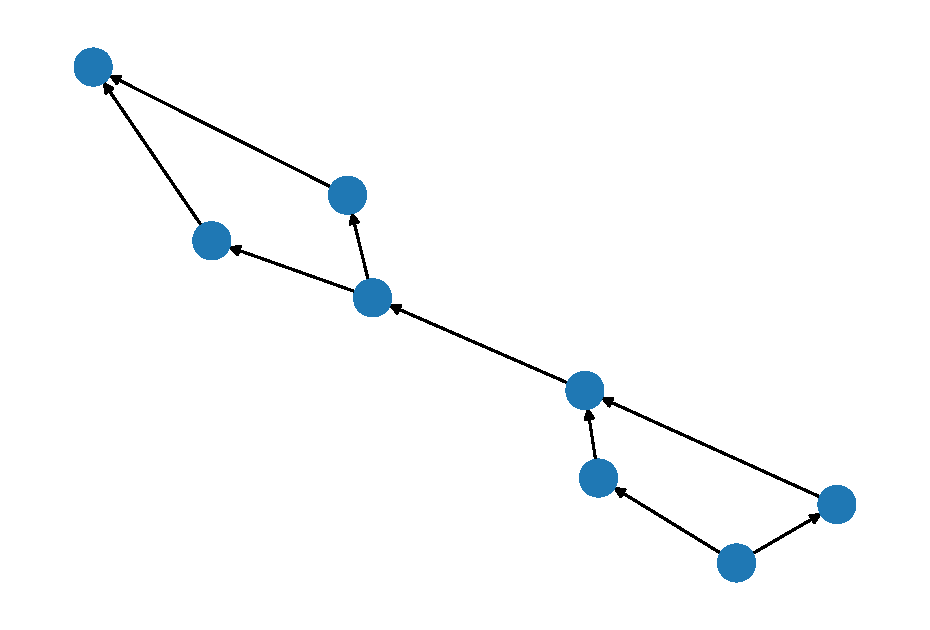
\includegraphics[width=0.3 \linewidth]{labs/figures/lab1_figure3_1.pdf}


\begin{minted}[mathescape, fontsize=\small, xleftmargin=0.5em]{python}
nx.draw(doubleFan(4))
\end{minted}
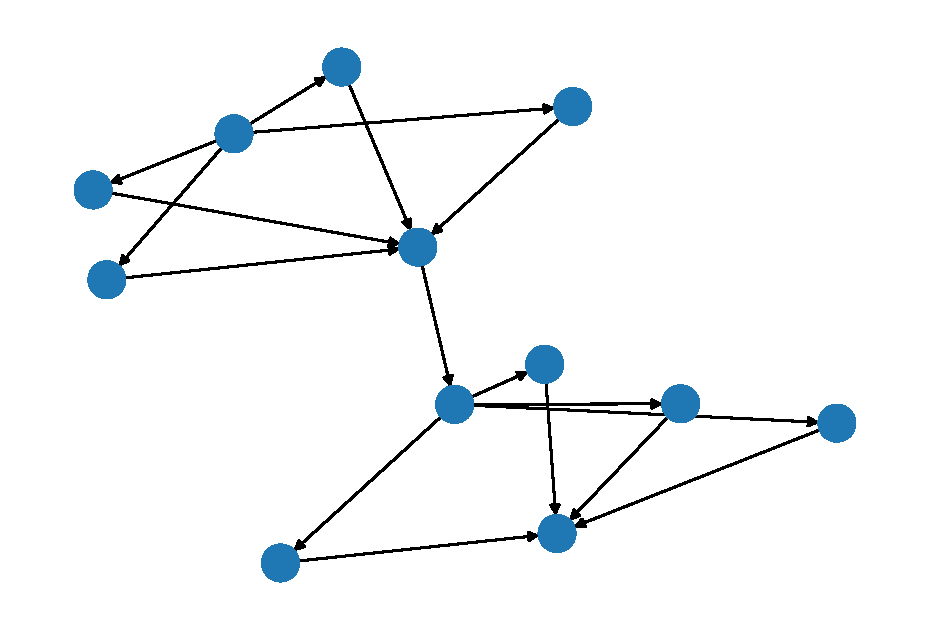
\includegraphics[width=0.3 \linewidth]{labs/figures/lab1_figure4_1.pdf}



\begin{minted}[mathescape, fontsize=\small, xleftmargin=0.5em]{python}
nx.draw(doubleFan(8))
\end{minted}
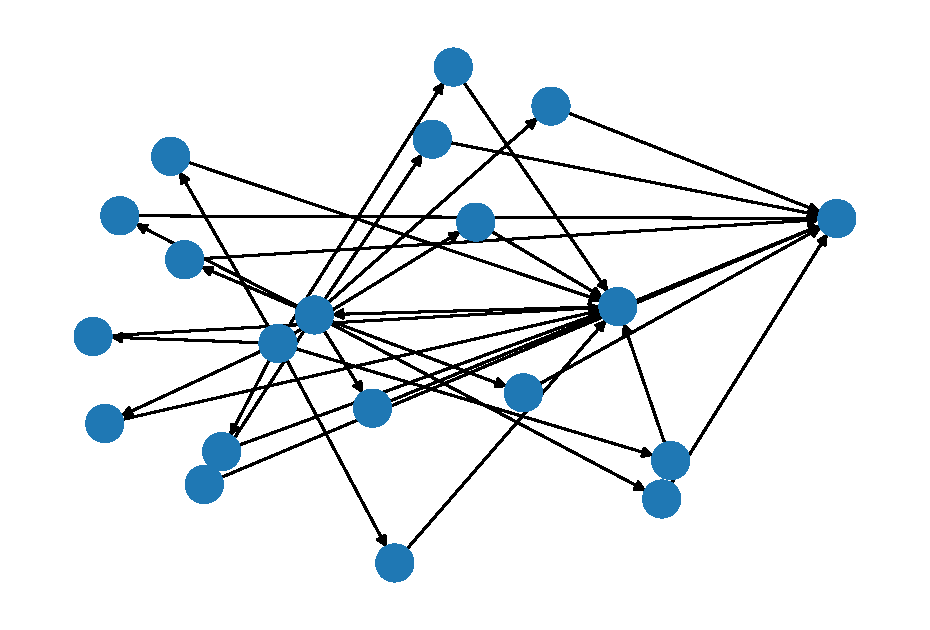
\includegraphics[width=0.3 \linewidth]{labs/figures/lab1_figure5_1.pdf}


Definiamo, quindi, una funzione che implementa \textsc{PricedDisjointPaths}: 


\begin{minted}[mathescape, fontsize=\small, xleftmargin=0.5em]{python}
def greedyDisjointPaths(G_original, sourceTargetPairs, c = 1):
    G = G_original.copy()
    result = []
    beta = math.pow(G.number_of_edges(), 1 / (c + 1))
    # Set all lengths to 1 and all congestion to 0
    for u,v,d in G.edges(data = True):
        d['length'] = 1
        d['congestion'] = 0
    # Main cycle
    while True:
        minPath = None
        for pairIndex in range(len(sourceTargetPairs)):
            try:
                source = sourceTargetPairs[pairIndex][0]
                target = sourceTargetPairs[pairIndex][1]
                path = dijkstra_path(G, source, target, 'length')
            except:
                pass
            else:
                pathLength = 0
                for i in range(len(path) - 1):
                    pathLength += G[path[i]][path[i+1]]['length']
                if minPath == None or pathLength < minPathLength:
                    minPath = path
                    minPathLength = pathLength
                    minPathIndex = pairIndex
        if minPath == None:
            break
        result.append(minPath)
        sourceTargetPairs.pop(minPathIndex)
        for i in range(len(path) - 1):
            x1 = path[i]
            x2 = path[i+1]
            G[x1][x2]['length'] *= beta
            G[x1][x2]['congestion'] += 1
            if G[x1][x2]['congestion'] == c:
                G.remove_edge(x1, x2)
    return result
\end{minted}



\begin{minted}[mathescape, fontsize=\small, xleftmargin=0.5em]{python}
g = doubleFan(2)
nx.draw(g, with_labels = True)
\end{minted}
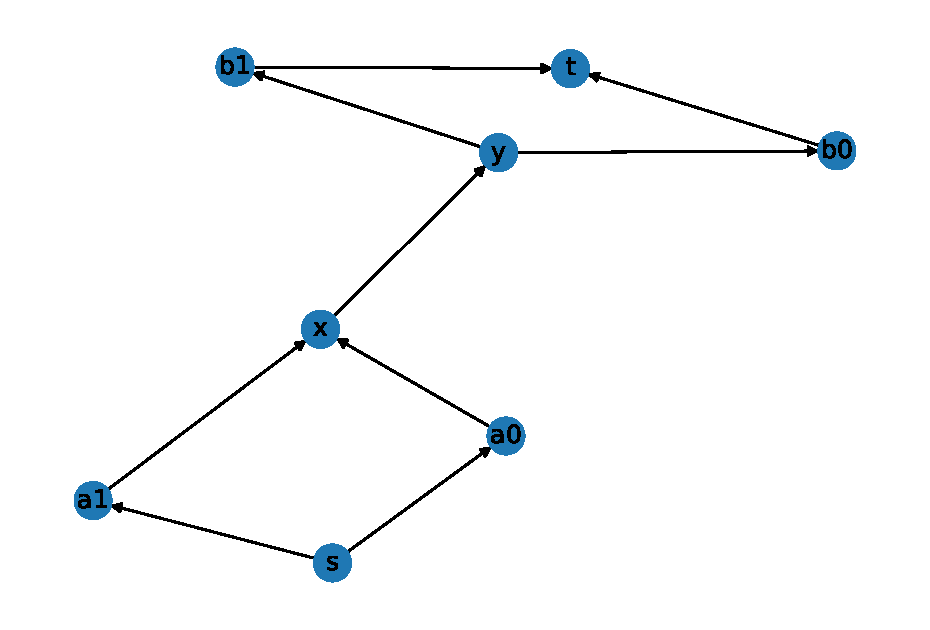
\includegraphics[width=0.5 \linewidth]{labs/figures/lab1_figure7_1.pdf}



\begin{minted}[mathescape, fontsize=\small, xleftmargin=0.5em]{python}
greedyDisjointPaths(g, [('s', 't')]*11, c = 10)
\end{minted}
\begin{minted}[fontsize=\small, xleftmargin=0.5em, mathescape, frame = leftline]{text}
[['s', 'a0', 'x', 'y', 'b0', 't'],
 ['s', 'a1', 'x', 'y', 'b1', 't'],
 ['s', 'a0', 'x', 'y', 'b0', 't'],
 ['s', 'a1', 'x', 'y', 'b1', 't'],
 ['s', 'a0', 'x', 'y', 'b0', 't'],
 ['s', 'a1', 'x', 'y', 'b1', 't'],
 ['s', 'a0', 'x', 'y', 'b0', 't'],
 ['s', 'a1', 'x', 'y', 'b1', 't'],
 ['s', 'a0', 'x', 'y', 'b0', 't'],
 ['s', 'a1', 'x', 'y', 'b1', 't']]
\end{minted}



\begin{minted}[mathescape, fontsize=\small, xleftmargin=0.5em]{python}
g = doubleFan(4)
nx.draw(g, with_labels = True)
\end{minted}
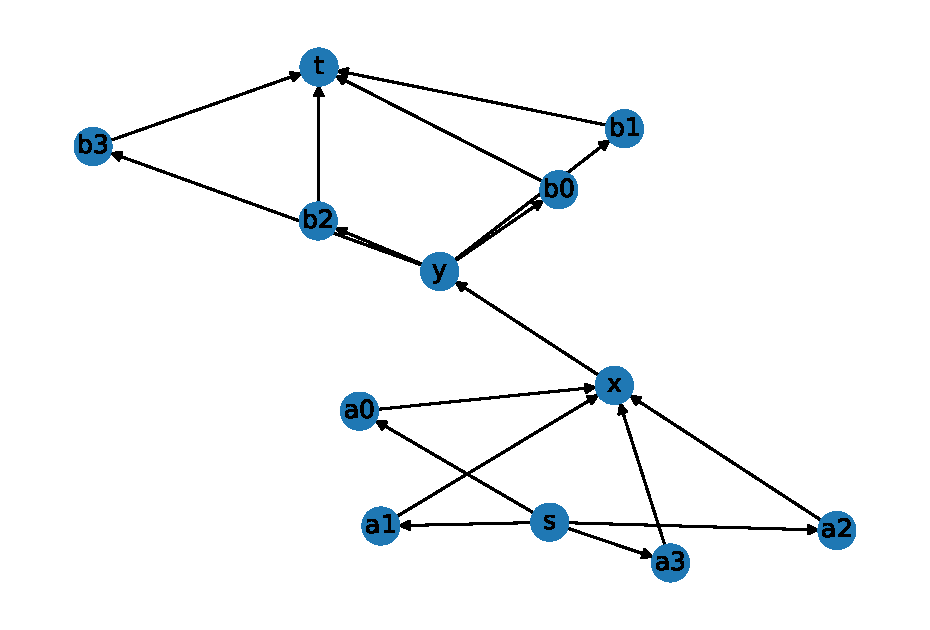
\includegraphics[width=0.5 \linewidth]{labs/figures/lab1_figure9_1.pdf}



\begin{minted}[mathescape, fontsize=\small, xleftmargin=0.5em]{python}
greedyDisjointPaths(g, [('s', 't')]*11, c = 10)
\end{minted}
\begin{minted}[fontsize=\small, xleftmargin=0.5em, mathescape, frame = leftline]{text}
[['s', 'a0', 'x', 'y', 'b0', 't'],
 ['s', 'a1', 'x', 'y', 'b1', 't'],
 ['s', 'a2', 'x', 'y', 'b2', 't'],
 ['s', 'a3', 'x', 'y', 'b3', 't'],
 ['s', 'a0', 'x', 'y', 'b0', 't'],
 ['s', 'a1', 'x', 'y', 'b1', 't'],
 ['s', 'a2', 'x', 'y', 'b2', 't'],
 ['s', 'a3', 'x', 'y', 'b3', 't'],
 ['s', 'a0', 'x', 'y', 'b0', 't'],
 ['s', 'a1', 'x', 'y', 'b1', 't']]
\end{minted}


\chapter{Laboratorio 2: il problema dello zaino}


\begin{minted}[mathescape, fontsize=\small, xleftmargin=0.5em]{python}
import numpy as np
import random
\end{minted}


Definiamo una funzione helper per creare istanze arbitrarie del problema: 


\begin{minted}[mathescape, fontsize=\small, xleftmargin=0.5em]{python}
# n is the number of objects to generate
# maxv is the maximum value
def generateInstance(n, maxv = 100):
    w = random.sample(range(1, maxv), n)
    v = random.sample(range(1, maxv), n)
    wBound = max(int(random.random() * maxv), max(w))
    return (list(zip(w, v)), wBound)
\end{minted}


Definiamo quindi il primo metodo basato sulla matrice dei valori $vOPT$. 

\begin{minted}[mathescape, fontsize=\small, xleftmargin=0.5em]{python}
# wv is a list of pairs (w,v)
# wBound is the capacity of the knapsack
# returns a pair (I, v) where v is the optimal value of a solution
# and I is the solution (set of indices)
def knapsackVopt(wv, wBound):
    n = len(wv)
    vOpt = np.zeros((n + 1, wBound + 1), int)
    for i in range(1, n + 1):
        vOpt[i][0] = 0
        for w in range(1, wBound + 1):
            currentItemWv = wv[i-1]
            currentW = currentItemWv[0]
            currentV = currentItemWv[1]
            if w >= currentW:
                vOpt[i][w] = max(vOpt[i-1][w], vOpt[i-1][w-currentW]+currentV)
            else:
                vOpt[i][w] = vOpt[i-1][w]
    I = []
    i = n
    w = wBound
    while i > 0:
        if vOpt[i-1,w] != vOpt[i, w]:
            I.append(i-1)
            w -= wv[i-1][0]
        i -= 1
    return (I,vOpt[n][wBound])
\end{minted}



\begin{minted}[mathescape, fontsize=\small, xleftmargin=0.5em]{python}
a = generateInstance(5, 10)
print(a)
print(knapsackVopt(*a))
\end{minted}
\begin{minted}[fontsize=\small, xleftmargin=0.5em, mathescape, frame = leftline]{text}
([(3, 4), (9, 8), (4, 9), (2, 6), (1, 3)], 9)
([3, 2, 0], 19)
\end{minted}


Definiamo il secondo metodo, basato sulla matrice di pesi $wOPT$. 

\begin{minted}[mathescape, fontsize=\small, xleftmargin=0.5em]{python}
# wv is a list of pairs (w,v)
# wBound is the capacity of the knapsack
# returns a pair (I, v) where v is the optimal value of a solution
# and I is the solution (set of indices)
def knapsackWopt(wv, wBound):
    n = len(wv)
    v = [wv[i][1] for i in range(n)]
    w = [wv[i][0] for i in range(n)]
    vMax = max(v)
    nvMax = n * vMax
    # Dynamic programming matrix
    wOpt = np.zeros((n + 1, nvMax + 1))
    print("Dimensione tabella: ", wOpt.nbytes)
    # Initialization
    for a in range(1, nvMax + 1):
        wOpt[0][a] = float('inf')
    # Filling
    for i in range(1, n + 1):
        wOpt[i][0] = 0
        for a in range(1, nvMax + 1):
            wOpt[i][a] = min(
                    wOpt[i - 1][a], 
                    wOpt[i - 1][max(a - v[i - 1], 0)] + w[i - 1])
    # Find the solution value a (on the last row)
    for a in range(nvMax, 0, -1):
        if wOpt[n][a] <= wBound:
            break
    # Reconstruct the solution
    finalV = a
    I = []
    i = n
    b = a
    while i > 0:
        if wOpt[i-1][b] != wOpt[i][b]:
            I.append(i-1)
            b -= v[i-1]
        i -= 1
    return (I,finalV)
\end{minted}


L'algoritmo $\mathbf{FPTAS}$ utilizza proprio quest'ultimo algoritmo appena definito: 

\begin{minted}[mathescape, fontsize=\small, xleftmargin=0.5em]{python}
from math import ceil
def knapsackFPTAS(wv, wBound, epsilon):
    n = len(wv)
    v = [wv[i][1] for i in range(n)]
    w = [wv[i][0] for i in range(n)]
    vMax = max(v)
    theta = max(epsilon * vMax / (2 * n), 1.0)
    vHat = [int(ceil(v[i] / theta)) for i in range(n)]
    print("Prima dell'arrotondamento: ", wv, wBound)
    print("Dopo l'arrotondamento: ", list(zip(w, vHat)), wBound)
    I, opt = knapsackWopt(list(zip(w, vHat)), wBound)
    vOpt = sum([v[i] for i in I])
    return I, vOpt
\end{minted}



\begin{minted}[mathescape, fontsize=\small, xleftmargin=0.5em]{python}
a = generateInstance(15, 10000)
Iexact, vexact = knapsackWopt(*a)
I, v = knapsackFPTAS(*a, 0.3)
print(Iexact, vexact)
print(I, v)
\end{minted}
\begin{minted}[fontsize=\small, xleftmargin=0.5em, mathescape, frame = leftline]{text}
Dimensione tabella:  17850368
Prima dell'arrotondamento:  [(1042, 3555), (9804, 9297), (376, 2780),
(2421, 277), (6697, 5289), (1202, 4197), (7569, 1164), (1896, 1082),
(1183, 7622), (1546, 1473), (7089, 6509), (3244, 4382), (8391, 1358),
(1373, 7811), (1454, 8170)] 9804
Dopo l'arrotondamento:  [(1042, 39), (9804, 100), (376, 30), (2421,
3), (6697, 57), (1202, 46), (7569, 13), (1896, 12), (1183, 82), (1546,
16), (7089, 71), (3244, 48), (8391, 15), (1373, 85), (1454, 88)] 9804
Dimensione tabella:  192128
[14, 13, 11, 8, 5, 0] 35737
[14, 13, 11, 8, 5, 0] 35737
\end{minted}



\backmatter
% if necessary, insert here your bibliography
\bibliographystyle{alpha}
\bibliography{bib/db}

\end{document}
